\documentclass[twoside]{book}

% Packages required by doxygen
\usepackage{fixltx2e}
\usepackage{calc}
\usepackage{doxygen}
\usepackage[export]{adjustbox} % also loads graphicx
\usepackage{graphicx}
\usepackage[utf8]{inputenc}
\usepackage{makeidx}
\usepackage{multicol}
\usepackage{multirow}
\PassOptionsToPackage{warn}{textcomp}
\usepackage{textcomp}
\usepackage[nointegrals]{wasysym}
\usepackage[table]{xcolor}

% Font selection
\usepackage[T1]{fontenc}
\usepackage[scaled=.90]{helvet}
\usepackage{courier}
\usepackage{amssymb}
\usepackage{sectsty}
\renewcommand{\familydefault}{\sfdefault}
\allsectionsfont{%
  \fontseries{bc}\selectfont%
  \color{darkgray}%
}
\renewcommand{\DoxyLabelFont}{%
  \fontseries{bc}\selectfont%
  \color{darkgray}%
}
\newcommand{\+}{\discretionary{\mbox{\scriptsize$\hookleftarrow$}}{}{}}

% Page & text layout
\usepackage{geometry}
\geometry{%
  a4paper,%
  top=2.5cm,%
  bottom=2.5cm,%
  left=2.5cm,%
  right=2.5cm%
}
\tolerance=750
\hfuzz=15pt
\hbadness=750
\setlength{\emergencystretch}{15pt}
\setlength{\parindent}{0cm}
\setlength{\parskip}{3ex plus 2ex minus 2ex}
\makeatletter
\renewcommand{\paragraph}{%
  \@startsection{paragraph}{4}{0ex}{-1.0ex}{1.0ex}{%
    \normalfont\normalsize\bfseries\SS@parafont%
  }%
}
\renewcommand{\subparagraph}{%
  \@startsection{subparagraph}{5}{0ex}{-1.0ex}{1.0ex}{%
    \normalfont\normalsize\bfseries\SS@subparafont%
  }%
}
\makeatother

% Headers & footers
\usepackage{fancyhdr}
\pagestyle{fancyplain}
\fancyhead[LE]{\fancyplain{}{\bfseries\thepage}}
\fancyhead[CE]{\fancyplain{}{}}
\fancyhead[RE]{\fancyplain{}{\bfseries\leftmark}}
\fancyhead[LO]{\fancyplain{}{\bfseries\rightmark}}
\fancyhead[CO]{\fancyplain{}{}}
\fancyhead[RO]{\fancyplain{}{\bfseries\thepage}}
\fancyfoot[LE]{\fancyplain{}{}}
\fancyfoot[CE]{\fancyplain{}{}}
\fancyfoot[RE]{\fancyplain{}{\bfseries\scriptsize Generated by Doxygen }}
\fancyfoot[LO]{\fancyplain{}{\bfseries\scriptsize Generated by Doxygen }}
\fancyfoot[CO]{\fancyplain{}{}}
\fancyfoot[RO]{\fancyplain{}{}}
\renewcommand{\footrulewidth}{0.4pt}
\renewcommand{\chaptermark}[1]{%
  \markboth{#1}{}%
}
\renewcommand{\sectionmark}[1]{%
  \markright{\thesection\ #1}%
}

% Indices & bibliography
\usepackage{natbib}
\usepackage[titles]{tocloft}
\setcounter{tocdepth}{3}
\setcounter{secnumdepth}{5}
\makeindex

% Hyperlinks (required, but should be loaded last)
\usepackage{ifpdf}
\ifpdf
  \usepackage[pdftex,pagebackref=true]{hyperref}
\else
  \usepackage[ps2pdf,pagebackref=true]{hyperref}
\fi
\hypersetup{%
  colorlinks=true,%
  linkcolor=blue,%
  citecolor=blue,%
  unicode%
}

% Custom commands
\newcommand{\clearemptydoublepage}{%
  \newpage{\pagestyle{empty}\cleardoublepage}%
}

\usepackage{caption}
\captionsetup{labelsep=space,justification=centering,font={bf},singlelinecheck=off,skip=4pt,position=top}

%===== C O N T E N T S =====

\begin{document}

% Titlepage & ToC
\hypersetup{pageanchor=false,
             bookmarksnumbered=true,
             pdfencoding=unicode
            }
\pagenumbering{alph}
\begin{titlepage}
\vspace*{7cm}
\begin{center}%
{\Large Codice Sistemi Embedded }\\
\vspace*{1cm}
{\large Generated by Doxygen 1.8.13}\\
\end{center}
\end{titlepage}
\clearemptydoublepage
\pagenumbering{roman}
\tableofcontents
\clearemptydoublepage
\pagenumbering{arabic}
\hypersetup{pageanchor=true}

%--- Begin generated contents ---
\chapter{Documentazione codice sistemi embedded}
\label{index}\hypertarget{index}{}\begin{DoxyParagraph}{Table of Contents}

\end{DoxyParagraph}
\hypertarget{index_GPIO}{}\section{G\+P\+IO}\label{index_GPIO}
\hypertarget{index_Driver}{}\subsection{Driver}\label{index_Driver}

\begin{DoxyItemize}
\item Funzioni driver G\+P\+IO \hyperlink{gpio__int_8c}{gpio\+\_\+int.\+c} 
\end{DoxyItemize}\hypertarget{index_Hardware}{}\subsection{Hardware}\label{index_Hardware}

\begin{DoxyItemize}
\item Controlla la generazione dell\textquotesingle{} interrupt \hyperlink{GPIO__v1__0__S00__AXI_8vhd}{G\+P\+I\+O\+\_\+v1\+\_\+0\+\_\+\+S00\+\_\+\+A\+X\+I.\+vhd}
\item Top level entity del componente \hyperlink{classGPIO__v1__0__S00__AXI}{G\+P\+I\+O\+\_\+v1\+\_\+0\+\_\+\+S00\+\_\+\+A\+XI} \hyperlink{GPIO__v1__0_8vhd}{G\+P\+I\+O\+\_\+v1\+\_\+0.\+vhd} 
\end{DoxyItemize}\hypertarget{index_UART}{}\section{U\+A\+RT}\label{index_UART}
\hypertarget{index_Driver}{}\subsection{Driver}\label{index_Driver}
\hypertarget{index_UIO}{}\subsubsection{U\+IO}\label{index_UIO}

\begin{DoxyItemize}
\item gestione del componente U\+A\+RT utilizzando il driver uio U\+A\+R\+T\+\_\+interrupt\+\_\+uio.\+c 
\end{DoxyItemize}\hypertarget{index_KERNEL}{}\subsubsection{K\+E\+R\+N\+EL}\label{index_KERNEL}

\begin{DoxyItemize}
\item gestione del componente U\+A\+RT in modalità kernel \hyperlink{UART__interrupt__kernel__mode_8c}{U\+A\+R\+T\+\_\+interrupt\+\_\+kernel\+\_\+mode.\+c} 
\end{DoxyItemize}\hypertarget{index_Hardware}{}\subsection{Hardware}\label{index_Hardware}

\begin{DoxyItemize}
\item Controlla la generazione dell\textquotesingle{} interrupt \hyperlink{UART__v1__0__S00__AXI_8vhd}{U\+A\+R\+T\+\_\+v1\+\_\+0\+\_\+\+S00\+\_\+\+A\+X\+I.\+vhd}
\item Top level entity del componente \hyperlink{classUART__v1__0__S00__AXI}{U\+A\+R\+T\+\_\+v1\+\_\+0\+\_\+\+S00\+\_\+\+A\+XI} \hyperlink{UART__v1__0_8vhd}{U\+A\+R\+T\+\_\+v1\+\_\+0.\+vhd} 
\end{DoxyItemize}\hypertarget{index_CRC}{}\section{C\+RC}\label{index_CRC}
@ F3
\begin{DoxyItemize}
\item gestione dell\textquotesingle{} invio, calcolo e check del C\+RC \hyperlink{STM32_2CRC__Revisited__loop_2src_2main_8c}{main.\+c} 
\end{DoxyItemize}
\chapter{driver\+\_\+\+G\+P\+IO}
\label{driver_GPIO}
\Hypertarget{driver_GPIO}
Funzioni per l\textquotesingle{}utilizzo della periferiferica \hyperlink{structGPIO}{G\+P\+IO} 
\chapter{driver\+\_\+\+U\+A\+R\+T\+\_\+kernel}
\label{driver_UART_kernel}
\Hypertarget{driver_UART_kernel}
funzioni per gestire la trasmissione e la ricezione dei dati utilizzando il protocollo U\+A\+RT (K\+E\+R\+N\+EL) 
\chapter{Module Index}
\section{Modules}
Here is a list of all modules\+:\begin{DoxyCompactList}
\item \contentsline{section}{S\+T\+M32\+F3xx\+\_\+\+H\+A\+L\+\_\+\+Examples}{\pageref{group__STM32F3xx__HAL__Examples}}{}
\begin{DoxyCompactList}
\item \contentsline{section}{U\+A\+R\+T\+\_\+\+Two\+Boards\+\_\+\+Com\+IT}{\pageref{group__UART__TwoBoards__ComIT}}{}
\begin{DoxyCompactList}
\item \contentsline{section}{H\+A\+L\+\_\+\+M\+S\+P\+\_\+\+Private\+\_\+\+Functions}{\pageref{group__HAL__MSP__Private__Functions}}{}
\end{DoxyCompactList}
\end{DoxyCompactList}
\item \contentsline{section}{C\+M\+S\+IS}{\pageref{group__CMSIS}}{}
\begin{DoxyCompactList}
\item \contentsline{section}{Stm32f3xx\+\_\+system}{\pageref{group__stm32f3xx__system}}{}
\begin{DoxyCompactList}
\item \contentsline{section}{S\+T\+M32\+F3xx\+\_\+\+System\+\_\+\+Private\+\_\+\+Includes}{\pageref{group__STM32F3xx__System__Private__Includes}}{}
\item \contentsline{section}{S\+T\+M32\+F3xx\+\_\+\+System\+\_\+\+Private\+\_\+\+Types\+Definitions}{\pageref{group__STM32F3xx__System__Private__TypesDefinitions}}{}
\item \contentsline{section}{S\+T\+M32\+F3xx\+\_\+\+System\+\_\+\+Private\+\_\+\+Defines}{\pageref{group__STM32F3xx__System__Private__Defines}}{}
\item \contentsline{section}{S\+T\+M32\+F3xx\+\_\+\+System\+\_\+\+Private\+\_\+\+Macros}{\pageref{group__STM32F3xx__System__Private__Macros}}{}
\item \contentsline{section}{S\+T\+M32\+F3xx\+\_\+\+System\+\_\+\+Private\+\_\+\+Variables}{\pageref{group__STM32F3xx__System__Private__Variables}}{}
\item \contentsline{section}{S\+T\+M32\+F3xx\+\_\+\+System\+\_\+\+Private\+\_\+\+Function\+Prototypes}{\pageref{group__STM32F3xx__System__Private__FunctionPrototypes}}{}
\item \contentsline{section}{S\+T\+M32\+F3xx\+\_\+\+System\+\_\+\+Private\+\_\+\+Functions}{\pageref{group__STM32F3xx__System__Private__Functions}}{}
\end{DoxyCompactList}
\end{DoxyCompactList}
\end{DoxyCompactList}

\chapter{Design Unit Index}
\section{Design Unit Hierarchy}
This inheritance list is sorted roughly, but not completely, alphabetically\+:\begin{DoxyCompactList}
\item \contentsline{section}{G\+P\+IO}{\pageref{structGPIO}}{}
\item \contentsline{section}{G\+P\+I\+O\+\_\+list}{\pageref{structGPIO__list}}{}
\item \contentsline{section}{G\+P\+I\+O\+\_\+v1\+\_\+0}{\pageref{classGPIO__v1__0}}{}
\begin{DoxyCompactList}
\item \contentsline{section}{G\+P\+I\+O\+\_\+v1\+\_\+0\+\_\+\+S00\+\_\+\+A\+XI}{\pageref{classGPIO__v1__0__S00__AXI}}{}
\end{DoxyCompactList}
\item \contentsline{section}{U\+A\+R\+T\+\_\+v1\+\_\+0}{\pageref{classUART__v1__0}}{}
\begin{DoxyCompactList}
\item \contentsline{section}{U\+A\+R\+T\+\_\+v1\+\_\+0\+\_\+\+S00\+\_\+\+A\+XI}{\pageref{classUART__v1__0__S00__AXI}}{}
\end{DoxyCompactList}
\end{DoxyCompactList}

\chapter{Design Unit Index}
\section{Design Unit List}
Here is a list of all design unit members with links to the Entities they belong to\+:\begin{DoxyCompactList}
\item\contentsline{section}{architecture \hyperlink{classGPIO__v1__0_1_1arch__imp}{arch\+\_\+imp} }{\pageref{classGPIO__v1__0_1_1arch__imp}}{}
\item\contentsline{section}{architecture \hyperlink{classGPIO__v1__0__S00__AXI_1_1arch__imp}{arch\+\_\+imp} }{\pageref{classGPIO__v1__0__S00__AXI_1_1arch__imp}}{}
\item\contentsline{section}{architecture \hyperlink{classUART__v1__0__S00__AXI_1_1arch__imp}{arch\+\_\+imp} }{\pageref{classUART__v1__0__S00__AXI_1_1arch__imp}}{}
\item\contentsline{section}{architecture \hyperlink{classUART__v1__0_1_1arch__imp}{arch\+\_\+imp} \\*Componente U\+A\+R\+T\+\_\+\+A\+X\+I\+\_\+\+S00  componente nel quale è incapsulato il componente U\+A\+RT e la logica di gestione delle interruzioni }{\pageref{classUART__v1__0_1_1arch__imp}}{}
\item\contentsline{section}{entity \hyperlink{classGPIO__v1__0}{G\+P\+I\+O\+\_\+v1\+\_\+0} }{\pageref{classGPIO__v1__0}}{}
\item\contentsline{section}{entity \hyperlink{classGPIO__v1__0__S00__AXI}{G\+P\+I\+O\+\_\+v1\+\_\+0\+\_\+\+S00\+\_\+\+A\+XI} }{\pageref{classGPIO__v1__0__S00__AXI}}{}
\item\contentsline{section}{\hyperlink{structmydriver__dm}{mydriver\+\_\+dm} }{\pageref{structmydriver__dm}}{}
\item\contentsline{section}{\hyperlink{structmyIntGPIO}{my\+Int\+G\+P\+IO} }{\pageref{structmyIntGPIO}}{}
\item\contentsline{section}{entity \hyperlink{classUART__v1__0}{U\+A\+R\+T\+\_\+v1\+\_\+0} }{\pageref{classUART__v1__0}}{}
\item\contentsline{section}{entity \hyperlink{classUART__v1__0__S00__AXI}{U\+A\+R\+T\+\_\+v1\+\_\+0\+\_\+\+S00\+\_\+\+A\+XI} }{\pageref{classUART__v1__0__S00__AXI}}{}
\end{DoxyCompactList}

\chapter{File Index}
\section{File List}
Here is a list of all documented files with brief descriptions\+:\begin{DoxyCompactList}
\item\contentsline{section}{/media/saverio/\+O\+S/\+Users/\+Saverio/\+Desktop/\+S\+E/git/\+Andrea/\+F\+P\+G\+A/\+G\+P\+I\+O\+With\+Interrupt/\+G\+P\+I\+O\+With\+Interrupt.\+sdk/\+G\+P\+I\+O/src/\hyperlink{gpio__int_8c}{gpio\+\_\+int.\+c} }{\pageref{gpio__int_8c}}{}
\item\contentsline{section}{/media/saverio/\+O\+S/\+Users/\+Saverio/\+Desktop/\+S\+E/git/\+Andrea/\+F\+P\+G\+A/\+G\+P\+I\+O\+With\+Interrupt/\+G\+P\+I\+O\+With\+Interrupt.\+sdk/\+G\+P\+I\+O/src/{\bfseries gpio\+\_\+int.\+h} }{\pageref{gpio__int_8h}}{}
\item\contentsline{section}{/media/saverio/\+O\+S/\+Users/\+Saverio/\+Desktop/\+S\+E/git/\+Andrea/\+F\+P\+G\+A/ip\+\_\+repo/\+G\+P\+I\+O\+\_\+1.\+0/hdl/\hyperlink{GPIO__v1__0_8vhd}{G\+P\+I\+O\+\_\+v1\+\_\+0.\+vhd} \\*Top level entity del custom IP core G\+P\+I\+O\+\_\+\+V1\+\_\+0\+\_\+\+S00\+\_\+\+A\+X\+I.\+V\+HD }{\pageref{GPIO__v1__0_8vhd}}{}
\item\contentsline{section}{/media/saverio/\+O\+S/\+Users/\+Saverio/\+Desktop/\+S\+E/git/\+Andrea/\+F\+P\+G\+A/ip\+\_\+repo/\+G\+P\+I\+O\+\_\+1.\+0/hdl/\hyperlink{GPIO__v1__0__S00__AXI_8vhd}{G\+P\+I\+O\+\_\+v1\+\_\+0\+\_\+\+S00\+\_\+\+A\+X\+I.\+vhd} \\*Componente utilizzato collegare il G\+P\+IO al bus A\+XI e gestire le interruzioni }{\pageref{GPIO__v1__0__S00__AXI_8vhd}}{}
\item\contentsline{section}{/media/saverio/\+O\+S/\+Users/\+Saverio/\+Desktop/\+S\+E/git/\+Andrea/\+F\+P\+G\+A/ip\+\_\+repo/\+U\+A\+R\+T\+\_\+1.\+0/hdl/\hyperlink{UART__v1__0_8vhd}{U\+A\+R\+T\+\_\+v1\+\_\+0.\+vhd} \\*U\+A\+RT A\+XI I\+P\+C\+O\+RE with interrupt }{\pageref{UART__v1__0_8vhd}}{}
\item\contentsline{section}{/media/saverio/\+O\+S/\+Users/\+Saverio/\+Desktop/\+S\+E/git/\+Andrea/\+F\+P\+G\+A/ip\+\_\+repo/\+U\+A\+R\+T\+\_\+1.\+0/hdl/\hyperlink{UART__v1__0__S00__AXI_8vhd}{U\+A\+R\+T\+\_\+v1\+\_\+0\+\_\+\+S00\+\_\+\+A\+X\+I.\+vhd} \\*U\+A\+RT A\+XI I\+P\+C\+O\+RE with interrupt }{\pageref{UART__v1__0__S00__AXI_8vhd}}{}
\end{DoxyCompactList}

\chapter{Module Documentation}
\hypertarget{group__UART__TwoBoards__ComIT}{}\section{U\+A\+R\+T\+\_\+\+Two\+Boards\+\_\+\+Com\+IT}
\label{group__UART__TwoBoards__ComIT}\index{U\+A\+R\+T\+\_\+\+Two\+Boards\+\_\+\+Com\+IT@{U\+A\+R\+T\+\_\+\+Two\+Boards\+\_\+\+Com\+IT}}
Collaboration diagram for U\+A\+R\+T\+\_\+\+Two\+Boards\+\_\+\+Com\+IT\+:\nopagebreak
\begin{figure}[H]
\begin{center}
\leavevmode
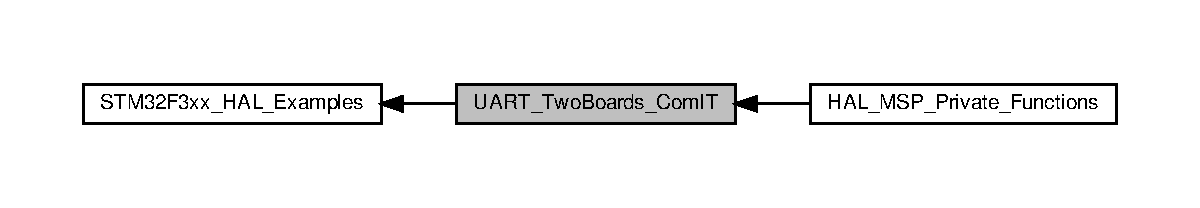
\includegraphics[width=350pt]{group__UART__TwoBoards__ComIT}
\end{center}
\end{figure}
\subsection*{Modules}
\begin{DoxyCompactItemize}
\item 
\hyperlink{group__HAL__MSP__Private__Functions}{H\+A\+L\+\_\+\+M\+S\+P\+\_\+\+Private\+\_\+\+Functions}
\end{DoxyCompactItemize}


\subsection{Detailed Description}


\subsection{Function Documentation}
\mbox{\Hypertarget{group__UART__TwoBoards__ComIT_ga2c27fc382a40cb4b92f9a48b327ab79f}\label{group__UART__TwoBoards__ComIT_ga2c27fc382a40cb4b92f9a48b327ab79f}} 
\index{U\+A\+R\+T\+\_\+\+Two\+Boards\+\_\+\+Com\+IT@{U\+A\+R\+T\+\_\+\+Two\+Boards\+\_\+\+Com\+IT}!Bus\+Fault\+\_\+\+Handler@{Bus\+Fault\+\_\+\+Handler}}
\index{Bus\+Fault\+\_\+\+Handler@{Bus\+Fault\+\_\+\+Handler}!U\+A\+R\+T\+\_\+\+Two\+Boards\+\_\+\+Com\+IT@{U\+A\+R\+T\+\_\+\+Two\+Boards\+\_\+\+Com\+IT}}
\subsubsection{\texorpdfstring{Bus\+Fault\+\_\+\+Handler()}{BusFault\_Handler()}}
{\footnotesize\ttfamily void Bus\+Fault\+\_\+\+Handler (\begin{DoxyParamCaption}\item[{void}]{ }\end{DoxyParamCaption})}



This function handles Bus Fault exception. 


\begin{DoxyParams}{Parameters}
{\em None} & \\
\hline
\end{DoxyParams}

\begin{DoxyRetVals}{Return values}
{\em None} & \\
\hline
\end{DoxyRetVals}
\mbox{\Hypertarget{group__UART__TwoBoards__ComIT_ga735f6cb6de12b1453d16db32dba3d2a8}\label{group__UART__TwoBoards__ComIT_ga735f6cb6de12b1453d16db32dba3d2a8}} 
\index{U\+A\+R\+T\+\_\+\+Two\+Boards\+\_\+\+Com\+IT@{U\+A\+R\+T\+\_\+\+Two\+Boards\+\_\+\+Com\+IT}!Debug\+Mon\+\_\+\+Handler@{Debug\+Mon\+\_\+\+Handler}}
\index{Debug\+Mon\+\_\+\+Handler@{Debug\+Mon\+\_\+\+Handler}!U\+A\+R\+T\+\_\+\+Two\+Boards\+\_\+\+Com\+IT@{U\+A\+R\+T\+\_\+\+Two\+Boards\+\_\+\+Com\+IT}}
\subsubsection{\texorpdfstring{Debug\+Mon\+\_\+\+Handler()}{DebugMon\_Handler()}}
{\footnotesize\ttfamily void Debug\+Mon\+\_\+\+Handler (\begin{DoxyParamCaption}\item[{void}]{ }\end{DoxyParamCaption})}



This function handles Debug Monitor exception. 


\begin{DoxyParams}{Parameters}
{\em None} & \\
\hline
\end{DoxyParams}

\begin{DoxyRetVals}{Return values}
{\em None} & \\
\hline
\end{DoxyRetVals}
\mbox{\Hypertarget{group__UART__TwoBoards__ComIT_gafd87c60b1444bdac059ec64438a07c9d}\label{group__UART__TwoBoards__ComIT_gafd87c60b1444bdac059ec64438a07c9d}} 
\index{U\+A\+R\+T\+\_\+\+Two\+Boards\+\_\+\+Com\+IT@{U\+A\+R\+T\+\_\+\+Two\+Boards\+\_\+\+Com\+IT}!E\+X\+T\+I0\+\_\+\+I\+R\+Q\+Handler@{E\+X\+T\+I0\+\_\+\+I\+R\+Q\+Handler}}
\index{E\+X\+T\+I0\+\_\+\+I\+R\+Q\+Handler@{E\+X\+T\+I0\+\_\+\+I\+R\+Q\+Handler}!U\+A\+R\+T\+\_\+\+Two\+Boards\+\_\+\+Com\+IT@{U\+A\+R\+T\+\_\+\+Two\+Boards\+\_\+\+Com\+IT}}
\subsubsection{\texorpdfstring{E\+X\+T\+I0\+\_\+\+I\+R\+Q\+Handler()}{EXTI0\_IRQHandler()}}
{\footnotesize\ttfamily void E\+X\+T\+I0\+\_\+\+I\+R\+Q\+Handler (\begin{DoxyParamCaption}\item[{void}]{ }\end{DoxyParamCaption})}



This function handles external line 0 interrupt request. 


\begin{DoxyParams}{Parameters}
{\em None} & \\
\hline
\end{DoxyParams}

\begin{DoxyRetVals}{Return values}
{\em None} & \\
\hline
\end{DoxyRetVals}
\mbox{\Hypertarget{group__UART__TwoBoards__ComIT_ga4a5138c64667901a5a25fb365f287b6d}\label{group__UART__TwoBoards__ComIT_ga4a5138c64667901a5a25fb365f287b6d}} 
\index{U\+A\+R\+T\+\_\+\+Two\+Boards\+\_\+\+Com\+IT@{U\+A\+R\+T\+\_\+\+Two\+Boards\+\_\+\+Com\+IT}!Hard\+Fault\+\_\+\+Handler@{Hard\+Fault\+\_\+\+Handler}}
\index{Hard\+Fault\+\_\+\+Handler@{Hard\+Fault\+\_\+\+Handler}!U\+A\+R\+T\+\_\+\+Two\+Boards\+\_\+\+Com\+IT@{U\+A\+R\+T\+\_\+\+Two\+Boards\+\_\+\+Com\+IT}}
\subsubsection{\texorpdfstring{Hard\+Fault\+\_\+\+Handler()}{HardFault\_Handler()}}
{\footnotesize\ttfamily void Hard\+Fault\+\_\+\+Handler (\begin{DoxyParamCaption}\item[{void}]{ }\end{DoxyParamCaption})}



This function handles Hard Fault exception. 


\begin{DoxyParams}{Parameters}
{\em None} & \\
\hline
\end{DoxyParams}

\begin{DoxyRetVals}{Return values}
{\em None} & \\
\hline
\end{DoxyRetVals}
\mbox{\Hypertarget{group__UART__TwoBoards__ComIT_ga0721f39c09b00b7bee9d7c3cfa41ec49}\label{group__UART__TwoBoards__ComIT_ga0721f39c09b00b7bee9d7c3cfa41ec49}} 
\index{U\+A\+R\+T\+\_\+\+Two\+Boards\+\_\+\+Com\+IT@{U\+A\+R\+T\+\_\+\+Two\+Boards\+\_\+\+Com\+IT}!Mem\+Manage\+\_\+\+Handler@{Mem\+Manage\+\_\+\+Handler}}
\index{Mem\+Manage\+\_\+\+Handler@{Mem\+Manage\+\_\+\+Handler}!U\+A\+R\+T\+\_\+\+Two\+Boards\+\_\+\+Com\+IT@{U\+A\+R\+T\+\_\+\+Two\+Boards\+\_\+\+Com\+IT}}
\subsubsection{\texorpdfstring{Mem\+Manage\+\_\+\+Handler()}{MemManage\_Handler()}}
{\footnotesize\ttfamily void Mem\+Manage\+\_\+\+Handler (\begin{DoxyParamCaption}\item[{void}]{ }\end{DoxyParamCaption})}



This function handles Memory Manage exception. 


\begin{DoxyParams}{Parameters}
{\em None} & \\
\hline
\end{DoxyParams}

\begin{DoxyRetVals}{Return values}
{\em None} & \\
\hline
\end{DoxyRetVals}
\mbox{\Hypertarget{group__UART__TwoBoards__ComIT_gaeddaa97a139c92c174f5fcccedc2859b}\label{group__UART__TwoBoards__ComIT_gaeddaa97a139c92c174f5fcccedc2859b}} 
\index{U\+A\+R\+T\+\_\+\+Two\+Boards\+\_\+\+Com\+IT@{U\+A\+R\+T\+\_\+\+Two\+Boards\+\_\+\+Com\+IT}!N\+M\+I\+\_\+\+Handler@{N\+M\+I\+\_\+\+Handler}}
\index{N\+M\+I\+\_\+\+Handler@{N\+M\+I\+\_\+\+Handler}!U\+A\+R\+T\+\_\+\+Two\+Boards\+\_\+\+Com\+IT@{U\+A\+R\+T\+\_\+\+Two\+Boards\+\_\+\+Com\+IT}}
\subsubsection{\texorpdfstring{N\+M\+I\+\_\+\+Handler()}{NMI\_Handler()}}
{\footnotesize\ttfamily void N\+M\+I\+\_\+\+Handler (\begin{DoxyParamCaption}\item[{void}]{ }\end{DoxyParamCaption})}



This function handles N\+MI exception. 


\begin{DoxyParams}{Parameters}
{\em None} & \\
\hline
\end{DoxyParams}

\begin{DoxyRetVals}{Return values}
{\em None} & \\
\hline
\end{DoxyRetVals}
\mbox{\Hypertarget{group__UART__TwoBoards__ComIT_ga6d82249321d9799b28fd83553671f901}\label{group__UART__TwoBoards__ComIT_ga6d82249321d9799b28fd83553671f901}} 
\index{U\+A\+R\+T\+\_\+\+Two\+Boards\+\_\+\+Com\+IT@{U\+A\+R\+T\+\_\+\+Two\+Boards\+\_\+\+Com\+IT}!Pend\+S\+V\+\_\+\+Handler@{Pend\+S\+V\+\_\+\+Handler}}
\index{Pend\+S\+V\+\_\+\+Handler@{Pend\+S\+V\+\_\+\+Handler}!U\+A\+R\+T\+\_\+\+Two\+Boards\+\_\+\+Com\+IT@{U\+A\+R\+T\+\_\+\+Two\+Boards\+\_\+\+Com\+IT}}
\subsubsection{\texorpdfstring{Pend\+S\+V\+\_\+\+Handler()}{PendSV\_Handler()}}
{\footnotesize\ttfamily void Pend\+S\+V\+\_\+\+Handler (\begin{DoxyParamCaption}\item[{void}]{ }\end{DoxyParamCaption})}



This function handles Pend\+S\+VC exception. 


\begin{DoxyParams}{Parameters}
{\em None} & \\
\hline
\end{DoxyParams}

\begin{DoxyRetVals}{Return values}
{\em None} & \\
\hline
\end{DoxyRetVals}
\mbox{\Hypertarget{group__UART__TwoBoards__ComIT_ga5e9cc540fdf30d55c5648d8e9f8f6013}\label{group__UART__TwoBoards__ComIT_ga5e9cc540fdf30d55c5648d8e9f8f6013}} 
\index{U\+A\+R\+T\+\_\+\+Two\+Boards\+\_\+\+Com\+IT@{U\+A\+R\+T\+\_\+\+Two\+Boards\+\_\+\+Com\+IT}!S\+V\+C\+\_\+\+Handler@{S\+V\+C\+\_\+\+Handler}}
\index{S\+V\+C\+\_\+\+Handler@{S\+V\+C\+\_\+\+Handler}!U\+A\+R\+T\+\_\+\+Two\+Boards\+\_\+\+Com\+IT@{U\+A\+R\+T\+\_\+\+Two\+Boards\+\_\+\+Com\+IT}}
\subsubsection{\texorpdfstring{S\+V\+C\+\_\+\+Handler()}{SVC\_Handler()}}
{\footnotesize\ttfamily void S\+V\+C\+\_\+\+Handler (\begin{DoxyParamCaption}\item[{void}]{ }\end{DoxyParamCaption})}



This function handles S\+V\+Call exception. 


\begin{DoxyParams}{Parameters}
{\em None} & \\
\hline
\end{DoxyParams}

\begin{DoxyRetVals}{Return values}
{\em None} & \\
\hline
\end{DoxyRetVals}
\mbox{\Hypertarget{group__UART__TwoBoards__ComIT_ga5380dd1db43723a5b8c5e57913886044}\label{group__UART__TwoBoards__ComIT_ga5380dd1db43723a5b8c5e57913886044}} 
\index{U\+A\+R\+T\+\_\+\+Two\+Boards\+\_\+\+Com\+IT@{U\+A\+R\+T\+\_\+\+Two\+Boards\+\_\+\+Com\+IT}!Sys\+Tick\+\_\+\+Handler@{Sys\+Tick\+\_\+\+Handler}}
\index{Sys\+Tick\+\_\+\+Handler@{Sys\+Tick\+\_\+\+Handler}!U\+A\+R\+T\+\_\+\+Two\+Boards\+\_\+\+Com\+IT@{U\+A\+R\+T\+\_\+\+Two\+Boards\+\_\+\+Com\+IT}}
\subsubsection{\texorpdfstring{Sys\+Tick\+\_\+\+Handler()}{SysTick\_Handler()}}
{\footnotesize\ttfamily void Sys\+Tick\+\_\+\+Handler (\begin{DoxyParamCaption}\item[{void}]{ }\end{DoxyParamCaption})}



This function handles Sys\+Tick Handler. 


\begin{DoxyParams}{Parameters}
{\em None} & \\
\hline
\end{DoxyParams}

\begin{DoxyRetVals}{Return values}
{\em None} & \\
\hline
\end{DoxyRetVals}
\mbox{\Hypertarget{group__UART__TwoBoards__ComIT_ga7640bb8e603ea919c8efb1ccecb0c8ef}\label{group__UART__TwoBoards__ComIT_ga7640bb8e603ea919c8efb1ccecb0c8ef}} 
\index{U\+A\+R\+T\+\_\+\+Two\+Boards\+\_\+\+Com\+IT@{U\+A\+R\+T\+\_\+\+Two\+Boards\+\_\+\+Com\+IT}!Usage\+Fault\+\_\+\+Handler@{Usage\+Fault\+\_\+\+Handler}}
\index{Usage\+Fault\+\_\+\+Handler@{Usage\+Fault\+\_\+\+Handler}!U\+A\+R\+T\+\_\+\+Two\+Boards\+\_\+\+Com\+IT@{U\+A\+R\+T\+\_\+\+Two\+Boards\+\_\+\+Com\+IT}}
\subsubsection{\texorpdfstring{Usage\+Fault\+\_\+\+Handler()}{UsageFault\_Handler()}}
{\footnotesize\ttfamily void Usage\+Fault\+\_\+\+Handler (\begin{DoxyParamCaption}\item[{void}]{ }\end{DoxyParamCaption})}



This function handles Usage Fault exception. 


\begin{DoxyParams}{Parameters}
{\em None} & \\
\hline
\end{DoxyParams}

\begin{DoxyRetVals}{Return values}
{\em None} & \\
\hline
\end{DoxyRetVals}
\mbox{\Hypertarget{group__UART__TwoBoards__ComIT_gabac2fe2ec91292dfc859adba560d24c3}\label{group__UART__TwoBoards__ComIT_gabac2fe2ec91292dfc859adba560d24c3}} 
\index{U\+A\+R\+T\+\_\+\+Two\+Boards\+\_\+\+Com\+IT@{U\+A\+R\+T\+\_\+\+Two\+Boards\+\_\+\+Com\+IT}!U\+S\+A\+R\+Tx\+\_\+\+I\+R\+Q\+Handler@{U\+S\+A\+R\+Tx\+\_\+\+I\+R\+Q\+Handler}}
\index{U\+S\+A\+R\+Tx\+\_\+\+I\+R\+Q\+Handler@{U\+S\+A\+R\+Tx\+\_\+\+I\+R\+Q\+Handler}!U\+A\+R\+T\+\_\+\+Two\+Boards\+\_\+\+Com\+IT@{U\+A\+R\+T\+\_\+\+Two\+Boards\+\_\+\+Com\+IT}}
\subsubsection{\texorpdfstring{U\+S\+A\+R\+Tx\+\_\+\+I\+R\+Q\+Handler()}{USARTx\_IRQHandler()}}
{\footnotesize\ttfamily void U\+S\+A\+R\+Tx\+\_\+\+I\+R\+Q\+Handler (\begin{DoxyParamCaption}\item[{void}]{ }\end{DoxyParamCaption})}



This function handles U\+A\+RT interrupt request. 


\begin{DoxyParams}{Parameters}
{\em None} & \\
\hline
\end{DoxyParams}

\begin{DoxyRetVals}{Return values}
{\em None} & This function is redefined in \char`\"{}main.\+h\char`\"{} and related to D\+MA used for U\+S\+A\+RT data transmission \\
\hline
\end{DoxyRetVals}

\hypertarget{group__HAL__MSP__Private__Functions}{}\section{H\+A\+L\+\_\+\+M\+S\+P\+\_\+\+Private\+\_\+\+Functions}
\label{group__HAL__MSP__Private__Functions}\index{H\+A\+L\+\_\+\+M\+S\+P\+\_\+\+Private\+\_\+\+Functions@{H\+A\+L\+\_\+\+M\+S\+P\+\_\+\+Private\+\_\+\+Functions}}
Collaboration diagram for H\+A\+L\+\_\+\+M\+S\+P\+\_\+\+Private\+\_\+\+Functions\+:\nopagebreak
\begin{figure}[H]
\begin{center}
\leavevmode
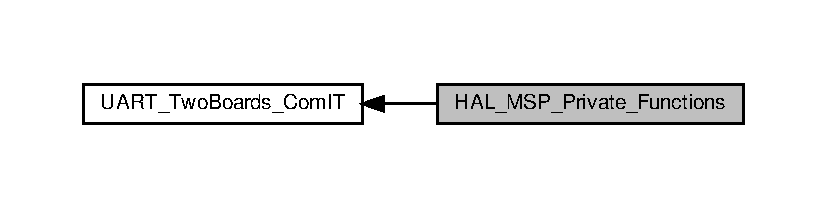
\includegraphics[width=350pt]{group__HAL__MSP__Private__Functions}
\end{center}
\end{figure}


\subsection{Detailed Description}


\subsection{Function Documentation}
\mbox{\Hypertarget{group__HAL__MSP__Private__Functions_ga8c3ca8029adb83e510a166b9b5022fb7}\label{group__HAL__MSP__Private__Functions_ga8c3ca8029adb83e510a166b9b5022fb7}} 
\index{H\+A\+L\+\_\+\+M\+S\+P\+\_\+\+Private\+\_\+\+Functions@{H\+A\+L\+\_\+\+M\+S\+P\+\_\+\+Private\+\_\+\+Functions}!H\+A\+L\+\_\+\+U\+A\+R\+T\+\_\+\+Msp\+De\+Init@{H\+A\+L\+\_\+\+U\+A\+R\+T\+\_\+\+Msp\+De\+Init}}
\index{H\+A\+L\+\_\+\+U\+A\+R\+T\+\_\+\+Msp\+De\+Init@{H\+A\+L\+\_\+\+U\+A\+R\+T\+\_\+\+Msp\+De\+Init}!H\+A\+L\+\_\+\+M\+S\+P\+\_\+\+Private\+\_\+\+Functions@{H\+A\+L\+\_\+\+M\+S\+P\+\_\+\+Private\+\_\+\+Functions}}
\subsubsection{\texorpdfstring{H\+A\+L\+\_\+\+U\+A\+R\+T\+\_\+\+Msp\+De\+Init()}{HAL\_UART\_MspDeInit()}}
{\footnotesize\ttfamily void H\+A\+L\+\_\+\+U\+A\+R\+T\+\_\+\+Msp\+De\+Init (\begin{DoxyParamCaption}\item[{U\+A\+R\+T\+\_\+\+Handle\+Type\+Def $\ast$}]{huart }\end{DoxyParamCaption})}



U\+A\+RT M\+SP De-\/\+Initialization This function frees the hardware resources used in this example\+: 


\begin{DoxyItemize}
\item Disable the Peripheral\textquotesingle{}s clock
\item Revert G\+P\+IO and N\+V\+IC configuration to their default state 
\begin{DoxyParams}{Parameters}
{\em huart} & U\+A\+RT handle pointer \\
\hline
\end{DoxyParams}

\begin{DoxyRetVals}{Return values}
{\em None} & \\
\hline
\end{DoxyRetVals}

\end{DoxyItemize}\mbox{\Hypertarget{group__HAL__MSP__Private__Functions_ga13f0f8431d6ec49733ccfa381972f0dd}\label{group__HAL__MSP__Private__Functions_ga13f0f8431d6ec49733ccfa381972f0dd}} 
\index{H\+A\+L\+\_\+\+M\+S\+P\+\_\+\+Private\+\_\+\+Functions@{H\+A\+L\+\_\+\+M\+S\+P\+\_\+\+Private\+\_\+\+Functions}!H\+A\+L\+\_\+\+U\+A\+R\+T\+\_\+\+Msp\+Init@{H\+A\+L\+\_\+\+U\+A\+R\+T\+\_\+\+Msp\+Init}}
\index{H\+A\+L\+\_\+\+U\+A\+R\+T\+\_\+\+Msp\+Init@{H\+A\+L\+\_\+\+U\+A\+R\+T\+\_\+\+Msp\+Init}!H\+A\+L\+\_\+\+M\+S\+P\+\_\+\+Private\+\_\+\+Functions@{H\+A\+L\+\_\+\+M\+S\+P\+\_\+\+Private\+\_\+\+Functions}}
\subsubsection{\texorpdfstring{H\+A\+L\+\_\+\+U\+A\+R\+T\+\_\+\+Msp\+Init()}{HAL\_UART\_MspInit()}}
{\footnotesize\ttfamily void H\+A\+L\+\_\+\+U\+A\+R\+T\+\_\+\+Msp\+Init (\begin{DoxyParamCaption}\item[{U\+A\+R\+T\+\_\+\+Handle\+Type\+Def $\ast$}]{huart }\end{DoxyParamCaption})}



U\+A\+RT M\+SP Initialization This function configures the hardware resources used in this example\+: 


\begin{DoxyItemize}
\item Peripheral\textquotesingle{}s clock enable
\item Peripheral\textquotesingle{}s G\+P\+IO Configuration
\item N\+V\+IC configuration for U\+A\+RT interrupt request enable 
\begin{DoxyParams}{Parameters}
{\em huart} & U\+A\+RT handle pointer \\
\hline
\end{DoxyParams}

\begin{DoxyRetVals}{Return values}
{\em None} & \\
\hline
\end{DoxyRetVals}

\end{DoxyItemize}
\hypertarget{group__STM32F3xx__HAL__Examples}{}\section{S\+T\+M32\+F3xx\+\_\+\+H\+A\+L\+\_\+\+Examples}
\label{group__STM32F3xx__HAL__Examples}\index{S\+T\+M32\+F3xx\+\_\+\+H\+A\+L\+\_\+\+Examples@{S\+T\+M32\+F3xx\+\_\+\+H\+A\+L\+\_\+\+Examples}}
Collaboration diagram for S\+T\+M32\+F3xx\+\_\+\+H\+A\+L\+\_\+\+Examples\+:\nopagebreak
\begin{figure}[H]
\begin{center}
\leavevmode
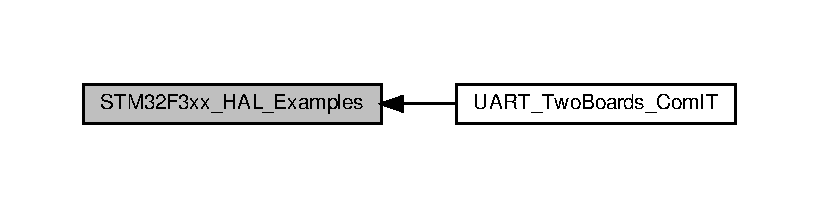
\includegraphics[width=350pt]{group__STM32F3xx__HAL__Examples}
\end{center}
\end{figure}
\subsection*{Modules}
\begin{DoxyCompactItemize}
\item 
\hyperlink{group__UART__TwoBoards__ComIT}{U\+A\+R\+T\+\_\+\+Two\+Boards\+\_\+\+Com\+IT}
\end{DoxyCompactItemize}


\subsection{Detailed Description}

\hypertarget{group__CMSIS}{}\section{C\+M\+S\+IS}
\label{group__CMSIS}\index{C\+M\+S\+IS@{C\+M\+S\+IS}}
Collaboration diagram for C\+M\+S\+IS\+:\nopagebreak
\begin{figure}[H]
\begin{center}
\leavevmode
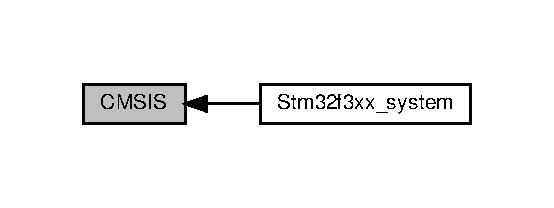
\includegraphics[width=266pt]{group__CMSIS}
\end{center}
\end{figure}
\subsection*{Modules}
\begin{DoxyCompactItemize}
\item 
\hyperlink{group__stm32f3xx__system}{Stm32f3xx\+\_\+system}
\end{DoxyCompactItemize}


\subsection{Detailed Description}

\hypertarget{group__stm32f3xx__system}{}\section{Stm32f3xx\+\_\+system}
\label{group__stm32f3xx__system}\index{Stm32f3xx\+\_\+system@{Stm32f3xx\+\_\+system}}
Collaboration diagram for Stm32f3xx\+\_\+system\+:\nopagebreak
\begin{figure}[H]
\begin{center}
\leavevmode
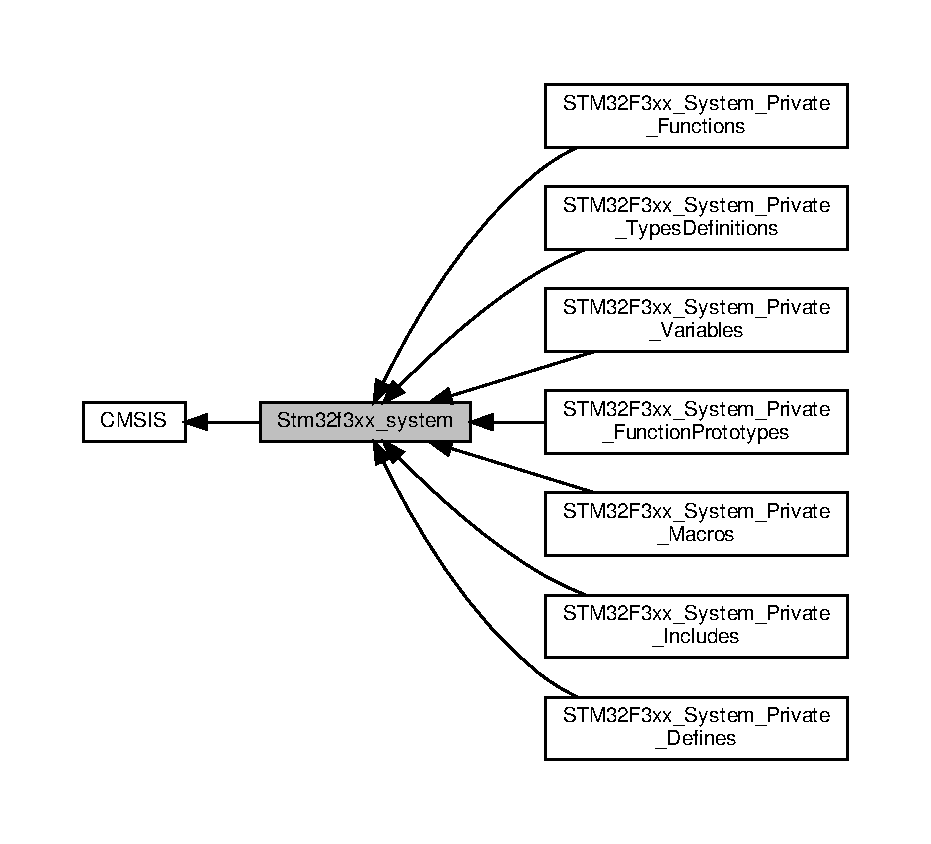
\includegraphics[width=350pt]{group__stm32f3xx__system}
\end{center}
\end{figure}
\subsection*{Modules}
\begin{DoxyCompactItemize}
\item 
\hyperlink{group__STM32F3xx__System__Private__Includes}{S\+T\+M32\+F3xx\+\_\+\+System\+\_\+\+Private\+\_\+\+Includes}
\item 
\hyperlink{group__STM32F3xx__System__Private__TypesDefinitions}{S\+T\+M32\+F3xx\+\_\+\+System\+\_\+\+Private\+\_\+\+Types\+Definitions}
\item 
\hyperlink{group__STM32F3xx__System__Private__Defines}{S\+T\+M32\+F3xx\+\_\+\+System\+\_\+\+Private\+\_\+\+Defines}
\item 
\hyperlink{group__STM32F3xx__System__Private__Macros}{S\+T\+M32\+F3xx\+\_\+\+System\+\_\+\+Private\+\_\+\+Macros}
\item 
\hyperlink{group__STM32F3xx__System__Private__Variables}{S\+T\+M32\+F3xx\+\_\+\+System\+\_\+\+Private\+\_\+\+Variables}
\item 
\hyperlink{group__STM32F3xx__System__Private__FunctionPrototypes}{S\+T\+M32\+F3xx\+\_\+\+System\+\_\+\+Private\+\_\+\+Function\+Prototypes}
\item 
\hyperlink{group__STM32F3xx__System__Private__Functions}{S\+T\+M32\+F3xx\+\_\+\+System\+\_\+\+Private\+\_\+\+Functions}
\end{DoxyCompactItemize}


\subsection{Detailed Description}

\hypertarget{group__STM32F3xx__System__Private__Includes}{}\section{S\+T\+M32\+F3xx\+\_\+\+System\+\_\+\+Private\+\_\+\+Includes}
\label{group__STM32F3xx__System__Private__Includes}\index{S\+T\+M32\+F3xx\+\_\+\+System\+\_\+\+Private\+\_\+\+Includes@{S\+T\+M32\+F3xx\+\_\+\+System\+\_\+\+Private\+\_\+\+Includes}}
Collaboration diagram for S\+T\+M32\+F3xx\+\_\+\+System\+\_\+\+Private\+\_\+\+Includes\+:\nopagebreak
\begin{figure}[H]
\begin{center}
\leavevmode
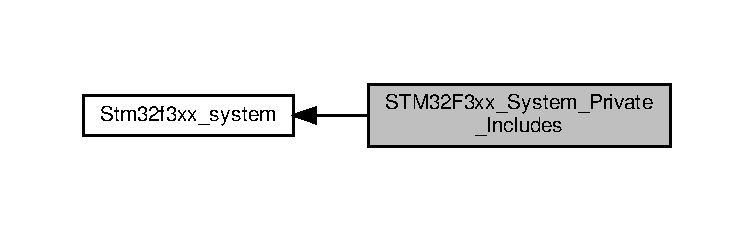
\includegraphics[width=350pt]{group__STM32F3xx__System__Private__Includes}
\end{center}
\end{figure}

\hypertarget{group__STM32F3xx__System__Private__TypesDefinitions}{}\section{S\+T\+M32\+F3xx\+\_\+\+System\+\_\+\+Private\+\_\+\+Types\+Definitions}
\label{group__STM32F3xx__System__Private__TypesDefinitions}\index{S\+T\+M32\+F3xx\+\_\+\+System\+\_\+\+Private\+\_\+\+Types\+Definitions@{S\+T\+M32\+F3xx\+\_\+\+System\+\_\+\+Private\+\_\+\+Types\+Definitions}}
Collaboration diagram for S\+T\+M32\+F3xx\+\_\+\+System\+\_\+\+Private\+\_\+\+Types\+Definitions\+:\nopagebreak
\begin{figure}[H]
\begin{center}
\leavevmode
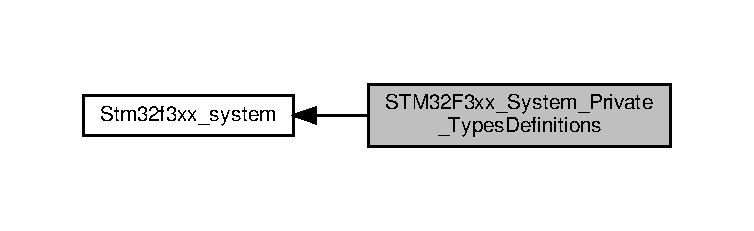
\includegraphics[width=350pt]{group__STM32F3xx__System__Private__TypesDefinitions}
\end{center}
\end{figure}

\hypertarget{group__STM32F3xx__System__Private__Defines}{}\section{S\+T\+M32\+F3xx\+\_\+\+System\+\_\+\+Private\+\_\+\+Defines}
\label{group__STM32F3xx__System__Private__Defines}\index{S\+T\+M32\+F3xx\+\_\+\+System\+\_\+\+Private\+\_\+\+Defines@{S\+T\+M32\+F3xx\+\_\+\+System\+\_\+\+Private\+\_\+\+Defines}}
Collaboration diagram for S\+T\+M32\+F3xx\+\_\+\+System\+\_\+\+Private\+\_\+\+Defines\+:\nopagebreak
\begin{figure}[H]
\begin{center}
\leavevmode
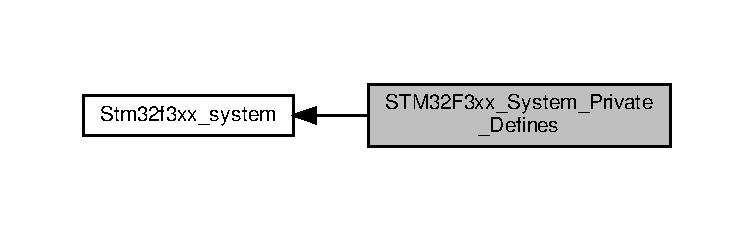
\includegraphics[width=350pt]{group__STM32F3xx__System__Private__Defines}
\end{center}
\end{figure}

\hypertarget{group__STM32F3xx__System__Private__Macros}{}\section{S\+T\+M32\+F3xx\+\_\+\+System\+\_\+\+Private\+\_\+\+Macros}
\label{group__STM32F3xx__System__Private__Macros}\index{S\+T\+M32\+F3xx\+\_\+\+System\+\_\+\+Private\+\_\+\+Macros@{S\+T\+M32\+F3xx\+\_\+\+System\+\_\+\+Private\+\_\+\+Macros}}
Collaboration diagram for S\+T\+M32\+F3xx\+\_\+\+System\+\_\+\+Private\+\_\+\+Macros\+:\nopagebreak
\begin{figure}[H]
\begin{center}
\leavevmode
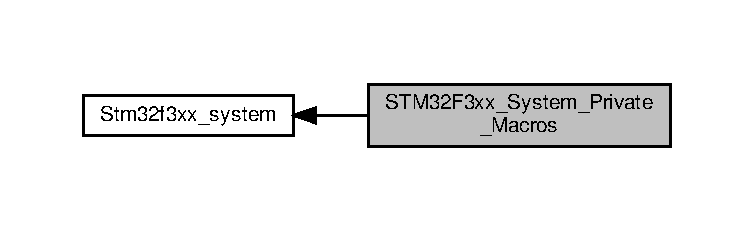
\includegraphics[width=350pt]{group__STM32F3xx__System__Private__Macros}
\end{center}
\end{figure}

\hypertarget{group__STM32F3xx__System__Private__Variables}{}\section{S\+T\+M32\+F3xx\+\_\+\+System\+\_\+\+Private\+\_\+\+Variables}
\label{group__STM32F3xx__System__Private__Variables}\index{S\+T\+M32\+F3xx\+\_\+\+System\+\_\+\+Private\+\_\+\+Variables@{S\+T\+M32\+F3xx\+\_\+\+System\+\_\+\+Private\+\_\+\+Variables}}
Collaboration diagram for S\+T\+M32\+F3xx\+\_\+\+System\+\_\+\+Private\+\_\+\+Variables\+:\nopagebreak
\begin{figure}[H]
\begin{center}
\leavevmode
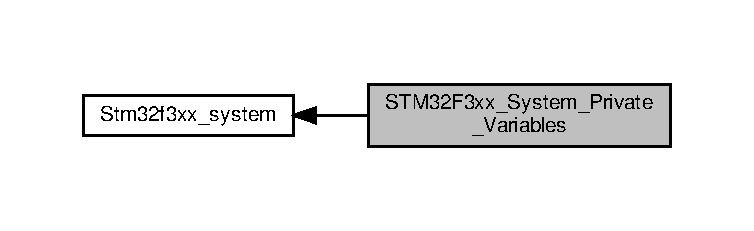
\includegraphics[width=350pt]{group__STM32F3xx__System__Private__Variables}
\end{center}
\end{figure}


\subsection{Detailed Description}

\hypertarget{group__STM32F3xx__System__Private__FunctionPrototypes}{}\section{S\+T\+M32\+F3xx\+\_\+\+System\+\_\+\+Private\+\_\+\+Function\+Prototypes}
\label{group__STM32F3xx__System__Private__FunctionPrototypes}\index{S\+T\+M32\+F3xx\+\_\+\+System\+\_\+\+Private\+\_\+\+Function\+Prototypes@{S\+T\+M32\+F3xx\+\_\+\+System\+\_\+\+Private\+\_\+\+Function\+Prototypes}}
Collaboration diagram for S\+T\+M32\+F3xx\+\_\+\+System\+\_\+\+Private\+\_\+\+Function\+Prototypes\+:\nopagebreak
\begin{figure}[H]
\begin{center}
\leavevmode
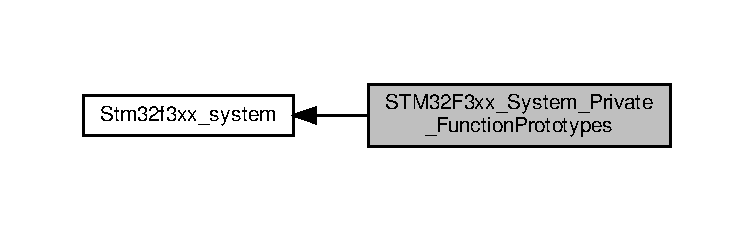
\includegraphics[width=350pt]{group__STM32F3xx__System__Private__FunctionPrototypes}
\end{center}
\end{figure}

\hypertarget{group__STM32F3xx__System__Private__Functions}{}\section{S\+T\+M32\+F3xx\+\_\+\+System\+\_\+\+Private\+\_\+\+Functions}
\label{group__STM32F3xx__System__Private__Functions}\index{S\+T\+M32\+F3xx\+\_\+\+System\+\_\+\+Private\+\_\+\+Functions@{S\+T\+M32\+F3xx\+\_\+\+System\+\_\+\+Private\+\_\+\+Functions}}
Collaboration diagram for S\+T\+M32\+F3xx\+\_\+\+System\+\_\+\+Private\+\_\+\+Functions\+:\nopagebreak
\begin{figure}[H]
\begin{center}
\leavevmode
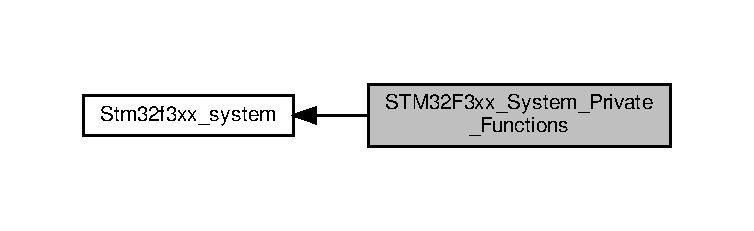
\includegraphics[width=350pt]{group__STM32F3xx__System__Private__Functions}
\end{center}
\end{figure}


\subsection{Detailed Description}


\subsection{Function Documentation}
\mbox{\Hypertarget{group__STM32F3xx__System__Private__Functions_ga19a0c3ef7421e9045e62d7df7f1120a9}\label{group__STM32F3xx__System__Private__Functions_ga19a0c3ef7421e9045e62d7df7f1120a9}} 
\index{S\+T\+M32\+F3xx\+\_\+\+System\+\_\+\+Private\+\_\+\+Functions@{S\+T\+M32\+F3xx\+\_\+\+System\+\_\+\+Private\+\_\+\+Functions}!System\+Core\+Clock\+Update@{System\+Core\+Clock\+Update}}
\index{System\+Core\+Clock\+Update@{System\+Core\+Clock\+Update}!S\+T\+M32\+F3xx\+\_\+\+System\+\_\+\+Private\+\_\+\+Functions@{S\+T\+M32\+F3xx\+\_\+\+System\+\_\+\+Private\+\_\+\+Functions}}
\subsubsection{\texorpdfstring{System\+Core\+Clock\+Update()}{SystemCoreClockUpdate()}}
{\footnotesize\ttfamily void System\+Core\+Clock\+Update (\begin{DoxyParamCaption}\item[{void}]{ }\end{DoxyParamCaption})}



Update System\+Core\+Clock variable according to Clock Register Values. The System\+Core\+Clock variable contains the core clock (H\+C\+LK), it can be used by the user application to setup the Sys\+Tick timer or configure other parameters. 

\begin{DoxyNote}{Note}
Each time the core clock (H\+C\+LK) changes, this function must be called to update System\+Core\+Clock variable value. Otherwise, any configuration based on this variable will be incorrect.

-\/ The system frequency computed by this function is not the real frequency in the chip. It is calculated based on the predefined constant and the selected clock source\+:
\end{DoxyNote}

\begin{DoxyItemize}
\item If S\+Y\+S\+C\+LK source is H\+SI, System\+Core\+Clock will contain the H\+S\+I\+\_\+\+V\+A\+L\+U\+E($\ast$)
\item If S\+Y\+S\+C\+LK source is H\+SE, System\+Core\+Clock will contain the H\+S\+E\+\_\+\+V\+A\+L\+U\+E($\ast$$\ast$)
\item If S\+Y\+S\+C\+LK source is P\+LL, System\+Core\+Clock will contain the H\+S\+E\+\_\+\+V\+A\+L\+U\+E($\ast$$\ast$) or H\+S\+I\+\_\+\+V\+A\+L\+U\+E($\ast$) multiplied/divided by the P\+LL factors.
\end{DoxyItemize}

($\ast$) H\+S\+I\+\_\+\+V\+A\+L\+UE is a constant defined in stm32f3xx\+\_\+hal.\+h file (default value 8 M\+Hz) but the real value may vary depending on the variations in voltage and temperature.

($\ast$$\ast$) H\+S\+E\+\_\+\+V\+A\+L\+UE is a constant defined in stm32f3xx\+\_\+hal.\+h file (default value 8 M\+Hz), user has to ensure that H\+S\+E\+\_\+\+V\+A\+L\+UE is same as the real frequency of the crystal used. Otherwise, this function may have wrong result.


\begin{DoxyItemize}
\item The result of this function could be not correct when using fractional value for H\+SE crystal.
\end{DoxyItemize}


\begin{DoxyParams}{Parameters}
{\em None} & \\
\hline
\end{DoxyParams}

\begin{DoxyRetVals}{Return values}
{\em None} & \\
\hline
\end{DoxyRetVals}
\mbox{\Hypertarget{group__STM32F3xx__System__Private__Functions_gaf019145746f780cda3053023bd6c1819}\label{group__STM32F3xx__System__Private__Functions_gaf019145746f780cda3053023bd6c1819}} 
\index{S\+T\+M32\+F3xx\+\_\+\+System\+\_\+\+Private\+\_\+\+Functions@{S\+T\+M32\+F3xx\+\_\+\+System\+\_\+\+Private\+\_\+\+Functions}!System\+Init@{System\+Init}}
\index{System\+Init@{System\+Init}!S\+T\+M32\+F3xx\+\_\+\+System\+\_\+\+Private\+\_\+\+Functions@{S\+T\+M32\+F3xx\+\_\+\+System\+\_\+\+Private\+\_\+\+Functions}}
\subsubsection{\texorpdfstring{System\+Init()}{SystemInit()}}
{\footnotesize\ttfamily void System\+Init (\begin{DoxyParamCaption}\item[{void}]{ }\end{DoxyParamCaption})}



Setup the microcontroller system Initialize the F\+PU setting, vector table location and the P\+LL configuration is reset. 


\begin{DoxyParams}{Parameters}
{\em None} & \\
\hline
\end{DoxyParams}

\begin{DoxyRetVals}{Return values}
{\em None} & \\
\hline
\end{DoxyRetVals}

\chapter{Data Structure Documentation}
\hypertarget{classGPIO__v1__0_1_1arch__imp}{}\section{arch\+\_\+imp Architecture Reference}
\label{classGPIO__v1__0_1_1arch__imp}\index{arch\+\_\+imp@{arch\+\_\+imp}}
\subsection*{Components}
 \begin{DoxyCompactItemize}
\item 
\mbox{\Hypertarget{classGPIO__v1__0_1_1arch__imp_acfa88fcc633c72af8bfd7e652932f7c7}\label{classGPIO__v1__0_1_1arch__imp_acfa88fcc633c72af8bfd7e652932f7c7}} 
\hyperlink{classGPIO__v1__0_1_1arch__imp_acfa88fcc633c72af8bfd7e652932f7c7}{G\+P\+I\+O\+\_\+v1\+\_\+0\+\_\+\+S00\+\_\+\+A\+XI}  {\bfseries }  
\end{DoxyCompactItemize}
\subsection*{Instantiations}
 \begin{DoxyCompactItemize}
\item 
\mbox{\Hypertarget{classGPIO__v1__0_1_1arch__imp_add7a292f6a3530426561c0d1bf9540b4}\label{classGPIO__v1__0_1_1arch__imp_add7a292f6a3530426561c0d1bf9540b4}} 
\hyperlink{classGPIO__v1__0_1_1arch__imp_add7a292f6a3530426561c0d1bf9540b4}{gpio\+\_\+v1\+\_\+0\+\_\+s00\+\_\+axi\+\_\+inst}  {\bfseries G\+P\+I\+O\+\_\+v1\+\_\+0\+\_\+\+S00\+\_\+\+A\+XI}   
\end{DoxyCompactItemize}


The documentation for this class was generated from the following file\+:\begin{DoxyCompactItemize}
\item 
/media/saverio/\+O\+S/\+Users/\+Saverio/\+Desktop/\+S\+E/git/\+Andrea/\+F\+P\+G\+A/ip\+\_\+repo/\+G\+P\+I\+O\+\_\+1.\+0/hdl/\hyperlink{GPIO__v1__0_8vhd}{G\+P\+I\+O\+\_\+v1\+\_\+0.\+vhd}\end{DoxyCompactItemize}

\hypertarget{classGPIO__v1__0__S00__AXI_1_1arch__imp}{}\section{arch\+\_\+imp Architecture Reference}
\label{classGPIO__v1__0__S00__AXI_1_1arch__imp}\index{arch\+\_\+imp@{arch\+\_\+imp}}
\subsection*{Processes}
 \begin{DoxyCompactItemize}
\item 
\mbox{\Hypertarget{classGPIO__v1__0__S00__AXI_1_1arch__imp_a655ff15956b68ed88b52a952f269c553}\label{classGPIO__v1__0__S00__AXI_1_1arch__imp_a655ff15956b68ed88b52a952f269c553}} 
\hyperlink{classGPIO__v1__0__S00__AXI_1_1arch__imp_a655ff15956b68ed88b52a952f269c553}{P\+R\+O\+C\+E\+S\+S\+\_\+0}{\bfseries  ( {\bfseries \textcolor{vhdlchar}{S\+\_\+\+A\+X\+I\+\_\+\+A\+C\+LK}\textcolor{vhdlchar}{ }} )}
\item 
\mbox{\Hypertarget{classGPIO__v1__0__S00__AXI_1_1arch__imp_a973f7a24b3f37478f610ab542f0e5086}\label{classGPIO__v1__0__S00__AXI_1_1arch__imp_a973f7a24b3f37478f610ab542f0e5086}} 
\hyperlink{classGPIO__v1__0__S00__AXI_1_1arch__imp_a973f7a24b3f37478f610ab542f0e5086}{P\+R\+O\+C\+E\+S\+S\+\_\+1}{\bfseries  ( {\bfseries \textcolor{vhdlchar}{S\+\_\+\+A\+X\+I\+\_\+\+A\+C\+LK}\textcolor{vhdlchar}{ }} )}
\item 
\mbox{\Hypertarget{classGPIO__v1__0__S00__AXI_1_1arch__imp_a5625666cb3140d01797433f2f6d93982}\label{classGPIO__v1__0__S00__AXI_1_1arch__imp_a5625666cb3140d01797433f2f6d93982}} 
\hyperlink{classGPIO__v1__0__S00__AXI_1_1arch__imp_a5625666cb3140d01797433f2f6d93982}{P\+R\+O\+C\+E\+S\+S\+\_\+2}{\bfseries  ( {\bfseries \textcolor{vhdlchar}{S\+\_\+\+A\+X\+I\+\_\+\+A\+C\+LK}\textcolor{vhdlchar}{ }} )}
\item 
\mbox{\Hypertarget{classGPIO__v1__0__S00__AXI_1_1arch__imp_a4bfd183cdd84fed1accdc6dcabc8fc3c}\label{classGPIO__v1__0__S00__AXI_1_1arch__imp_a4bfd183cdd84fed1accdc6dcabc8fc3c}} 
\hyperlink{classGPIO__v1__0__S00__AXI_1_1arch__imp_a4bfd183cdd84fed1accdc6dcabc8fc3c}{P\+R\+O\+C\+E\+S\+S\+\_\+3}{\bfseries  ( {\bfseries \textcolor{vhdlchar}{S\+\_\+\+A\+X\+I\+\_\+\+A\+C\+LK}\textcolor{vhdlchar}{ }} )}
\item 
\mbox{\Hypertarget{classGPIO__v1__0__S00__AXI_1_1arch__imp_a78c6c876515e14c79fe38dcb286ce0f1}\label{classGPIO__v1__0__S00__AXI_1_1arch__imp_a78c6c876515e14c79fe38dcb286ce0f1}} 
\hyperlink{classGPIO__v1__0__S00__AXI_1_1arch__imp_a78c6c876515e14c79fe38dcb286ce0f1}{P\+R\+O\+C\+E\+S\+S\+\_\+4}{\bfseries  ( {\bfseries \textcolor{vhdlchar}{S\+\_\+\+A\+X\+I\+\_\+\+A\+C\+LK}\textcolor{vhdlchar}{ }} )}
\item 
\mbox{\Hypertarget{classGPIO__v1__0__S00__AXI_1_1arch__imp_aeef87657fc8d27430790f1e6088ab81f}\label{classGPIO__v1__0__S00__AXI_1_1arch__imp_aeef87657fc8d27430790f1e6088ab81f}} 
\hyperlink{classGPIO__v1__0__S00__AXI_1_1arch__imp_aeef87657fc8d27430790f1e6088ab81f}{P\+R\+O\+C\+E\+S\+S\+\_\+5}{\bfseries  ( {\bfseries \textcolor{vhdlchar}{S\+\_\+\+A\+X\+I\+\_\+\+A\+C\+LK}\textcolor{vhdlchar}{ }} )}
\item 
\mbox{\Hypertarget{classGPIO__v1__0__S00__AXI_1_1arch__imp_a7390c9b34974c278e7646b784061d076}\label{classGPIO__v1__0__S00__AXI_1_1arch__imp_a7390c9b34974c278e7646b784061d076}} 
\hyperlink{classGPIO__v1__0__S00__AXI_1_1arch__imp_a7390c9b34974c278e7646b784061d076}{P\+R\+O\+C\+E\+S\+S\+\_\+6}{\bfseries  ( {\bfseries \textcolor{vhdlchar}{S\+\_\+\+A\+X\+I\+\_\+\+A\+C\+LK}\textcolor{vhdlchar}{ }} )}
\item 
\mbox{\Hypertarget{classGPIO__v1__0__S00__AXI_1_1arch__imp_a7eca128197092fa81fcaaba67313360f}\label{classGPIO__v1__0__S00__AXI_1_1arch__imp_a7eca128197092fa81fcaaba67313360f}} 
\hyperlink{classGPIO__v1__0__S00__AXI_1_1arch__imp_a7eca128197092fa81fcaaba67313360f}{P\+R\+O\+C\+E\+S\+S\+\_\+7}{\bfseries  ( {\bfseries \textcolor{vhdlchar}{slv\+\_\+reg0}\textcolor{vhdlchar}{ }} , {\bfseries \textcolor{vhdlchar}{slv\+\_\+reg1}\textcolor{vhdlchar}{ }} , {\bfseries \textcolor{vhdlchar}{gpio\+\_\+read}\textcolor{vhdlchar}{ }} , {\bfseries \textcolor{vhdlchar}{slv\+\_\+reg3}\textcolor{vhdlchar}{ }} , {\bfseries \textcolor{vhdlchar}{slv\+\_\+reg4}\textcolor{vhdlchar}{ }} , {\bfseries \textcolor{vhdlchar}{slv\+\_\+reg5}\textcolor{vhdlchar}{ }} , {\bfseries \textcolor{vhdlchar}{status\+\_\+reg\+\_\+out}\textcolor{vhdlchar}{ }} , {\bfseries \textcolor{vhdlchar}{slv\+\_\+reg7\+\_\+out}\textcolor{vhdlchar}{ }} , {\bfseries \textcolor{vhdlchar}{axi\+\_\+araddr}\textcolor{vhdlchar}{ }} , {\bfseries \textcolor{vhdlchar}{S\+\_\+\+A\+X\+I\+\_\+\+A\+R\+E\+S\+E\+TN}\textcolor{vhdlchar}{ }} , {\bfseries \textcolor{vhdlchar}{slv\+\_\+reg\+\_\+rden}\textcolor{vhdlchar}{ }} )}
\item 
\mbox{\Hypertarget{classGPIO__v1__0__S00__AXI_1_1arch__imp_a45eef1701e94703c5a3cf169c02e5e2c}\label{classGPIO__v1__0__S00__AXI_1_1arch__imp_a45eef1701e94703c5a3cf169c02e5e2c}} 
\hyperlink{classGPIO__v1__0__S00__AXI_1_1arch__imp_a45eef1701e94703c5a3cf169c02e5e2c}{P\+R\+O\+C\+E\+S\+S\+\_\+8}{\bfseries  ( {\bfseries \textcolor{vhdlchar}{S\+\_\+\+A\+X\+I\+\_\+\+A\+C\+LK}\textcolor{vhdlchar}{ }} )}
\item 
\hyperlink{classGPIO__v1__0__S00__AXI_1_1arch__imp_a29a70265aec87dff63669cc686cdd7b6}{gpio\+\_\+read\+\_\+sampling}{\bfseries  ( {\bfseries \textcolor{vhdlchar}{S\+\_\+\+A\+X\+I\+\_\+\+A\+C\+LK}\textcolor{vhdlchar}{ }} , {\bfseries \textcolor{vhdlchar}{gpio\+\_\+read}\textcolor{vhdlchar}{ }} )}
\begin{DoxyCompactList}\small\item\em Campiona i segnali di cui si vuole verificare la generazione di un interrupt. \end{DoxyCompactList}\item 
\hyperlink{classGPIO__v1__0__S00__AXI_1_1arch__imp_a27a13ac4e8c3307360aa906035c2e140}{intr\+\_\+pending}{\bfseries  ( {\bfseries \textcolor{vhdlchar}{S\+\_\+\+A\+X\+I\+\_\+\+A\+C\+LK}\textcolor{vhdlchar}{ }} , {\bfseries \textcolor{vhdlchar}{change\+\_\+detected}\textcolor{vhdlchar}{ }} , {\bfseries \textcolor{vhdlchar}{ack\+\_\+intr}\textcolor{vhdlchar}{ }} , {\bfseries \textcolor{vhdlchar}{pending\+\_\+intr\+\_\+tmp}\textcolor{vhdlchar}{ }} )}
\begin{DoxyCompactList}\small\item\em Gestisce il registro pending. \end{DoxyCompactList}\item 
\hyperlink{classGPIO__v1__0__S00__AXI_1_1arch__imp_ad49f0dfc577739899b90a7243c22a1cd}{inst\+\_\+irq}{\bfseries  ( {\bfseries \textcolor{vhdlchar}{S\+\_\+\+A\+X\+I\+\_\+\+A\+C\+LK}\textcolor{vhdlchar}{ }} , {\bfseries \textcolor{vhdlchar}{pending\+\_\+intr}\textcolor{vhdlchar}{ }} , {\bfseries \textcolor{vhdlchar}{global\+\_\+intr}\textcolor{vhdlchar}{ }} )}
\begin{DoxyCompactList}\small\item\em Disabilita l\textquotesingle{} interrupt nel caso di reset del bus e tiene alto il segnale di interrupt finchè rimane pendente. \end{DoxyCompactList}\end{DoxyCompactItemize}
\subsection*{Components}
 \begin{DoxyCompactItemize}
\item 
\mbox{\Hypertarget{classGPIO__v1__0__S00__AXI_1_1arch__imp_a7f7f55a1fb49e8857e13928560e7c192}\label{classGPIO__v1__0__S00__AXI_1_1arch__imp_a7f7f55a1fb49e8857e13928560e7c192}} 
\hyperlink{classGPIO__v1__0__S00__AXI_1_1arch__imp_a7f7f55a1fb49e8857e13928560e7c192}{G\+P\+I\+O\+\_\+\+Array}  {\bfseries }  
\end{DoxyCompactItemize}
\subsection*{Constants}
 \begin{DoxyCompactItemize}
\item 
\mbox{\Hypertarget{classGPIO__v1__0__S00__AXI_1_1arch__imp_a92f00d1b43f901f1bf5684d1e79aab84}\label{classGPIO__v1__0__S00__AXI_1_1arch__imp_a92f00d1b43f901f1bf5684d1e79aab84}} 
\hyperlink{classGPIO__v1__0__S00__AXI_1_1arch__imp_a92f00d1b43f901f1bf5684d1e79aab84}{A\+D\+D\+R\+\_\+\+L\+SB} {\bfseries \textcolor{vhdlchar}{integer}\textcolor{vhdlchar}{ }\textcolor{vhdlchar}{ }\textcolor{vhdlchar}{\+:}\textcolor{vhdlchar}{=}\textcolor{vhdlchar}{ }\textcolor{vhdlchar}{(}\textcolor{vhdlchar}{ }\textcolor{vhdlchar}{ }\textcolor{vhdlchar}{ }\textcolor{vhdlchar}{ }\textcolor{vhdlchar}{C\+\_\+\+S\+\_\+\+A\+X\+I\+\_\+\+D\+A\+T\+A\+\_\+\+W\+I\+D\+TH}\textcolor{vhdlchar}{/}\textcolor{vhdlchar}{ } \textcolor{vhdldigit}{32} \textcolor{vhdlchar}{ }\textcolor{vhdlchar}{)}\textcolor{vhdlchar}{ }\textcolor{vhdlchar}{+}\textcolor{vhdlchar}{ } \textcolor{vhdldigit}{1} \textcolor{vhdlchar}{ }} 
\item 
\mbox{\Hypertarget{classGPIO__v1__0__S00__AXI_1_1arch__imp_a913a8d777fcc731ba920264a143ec91f}\label{classGPIO__v1__0__S00__AXI_1_1arch__imp_a913a8d777fcc731ba920264a143ec91f}} 
\hyperlink{classGPIO__v1__0__S00__AXI_1_1arch__imp_a913a8d777fcc731ba920264a143ec91f}{O\+P\+T\+\_\+\+M\+E\+M\+\_\+\+A\+D\+D\+R\+\_\+\+B\+I\+TS} {\bfseries \textcolor{vhdlchar}{integer}\textcolor{vhdlchar}{ }\textcolor{vhdlchar}{ }\textcolor{vhdlchar}{\+:}\textcolor{vhdlchar}{=}\textcolor{vhdlchar}{ }\textcolor{vhdlchar}{ } \textcolor{vhdldigit}{2} \textcolor{vhdlchar}{ }} 
\end{DoxyCompactItemize}
\subsection*{Signals}
 \begin{DoxyCompactItemize}
\item 
\mbox{\Hypertarget{classGPIO__v1__0__S00__AXI_1_1arch__imp_ac022af52d7126cf515130cdd10e089fc}\label{classGPIO__v1__0__S00__AXI_1_1arch__imp_ac022af52d7126cf515130cdd10e089fc}} 
\hyperlink{classGPIO__v1__0__S00__AXI_1_1arch__imp_ac022af52d7126cf515130cdd10e089fc}{axi\+\_\+awaddr} {\bfseries \textcolor{vhdlchar}{std\+\_\+logic\+\_\+vector}\textcolor{vhdlchar}{ }\textcolor{vhdlchar}{(}\textcolor{vhdlchar}{ }\textcolor{vhdlchar}{ }\textcolor{vhdlchar}{ }\textcolor{vhdlchar}{ }\textcolor{vhdlchar}{C\+\_\+\+S\+\_\+\+A\+X\+I\+\_\+\+A\+D\+D\+R\+\_\+\+W\+I\+D\+TH}\textcolor{vhdlchar}{-\/}\textcolor{vhdlchar}{ } \textcolor{vhdldigit}{1} \textcolor{vhdlchar}{ }\textcolor{vhdlchar}{downto}\textcolor{vhdlchar}{ }\textcolor{vhdlchar}{ } \textcolor{vhdldigit}{0} \textcolor{vhdlchar}{ }\textcolor{vhdlchar}{)}\textcolor{vhdlchar}{ }} 
\item 
\mbox{\Hypertarget{classGPIO__v1__0__S00__AXI_1_1arch__imp_abe920675e5bffe2b708237782acd713d}\label{classGPIO__v1__0__S00__AXI_1_1arch__imp_abe920675e5bffe2b708237782acd713d}} 
\hyperlink{classGPIO__v1__0__S00__AXI_1_1arch__imp_abe920675e5bffe2b708237782acd713d}{axi\+\_\+awready} {\bfseries \textcolor{vhdlchar}{std\+\_\+logic}\textcolor{vhdlchar}{ }} 
\item 
\mbox{\Hypertarget{classGPIO__v1__0__S00__AXI_1_1arch__imp_a65364960779319dfc2c67e7d943d0499}\label{classGPIO__v1__0__S00__AXI_1_1arch__imp_a65364960779319dfc2c67e7d943d0499}} 
\hyperlink{classGPIO__v1__0__S00__AXI_1_1arch__imp_a65364960779319dfc2c67e7d943d0499}{axi\+\_\+wready} {\bfseries \textcolor{vhdlchar}{std\+\_\+logic}\textcolor{vhdlchar}{ }} 
\item 
\mbox{\Hypertarget{classGPIO__v1__0__S00__AXI_1_1arch__imp_ae5e5ea90e34af927db9507875d261a1a}\label{classGPIO__v1__0__S00__AXI_1_1arch__imp_ae5e5ea90e34af927db9507875d261a1a}} 
\hyperlink{classGPIO__v1__0__S00__AXI_1_1arch__imp_ae5e5ea90e34af927db9507875d261a1a}{axi\+\_\+bresp} {\bfseries \textcolor{vhdlchar}{std\+\_\+logic\+\_\+vector}\textcolor{vhdlchar}{ }\textcolor{vhdlchar}{(}\textcolor{vhdlchar}{ }\textcolor{vhdlchar}{ } \textcolor{vhdldigit}{1} \textcolor{vhdlchar}{ }\textcolor{vhdlchar}{downto}\textcolor{vhdlchar}{ }\textcolor{vhdlchar}{ } \textcolor{vhdldigit}{0} \textcolor{vhdlchar}{ }\textcolor{vhdlchar}{)}\textcolor{vhdlchar}{ }} 
\item 
\mbox{\Hypertarget{classGPIO__v1__0__S00__AXI_1_1arch__imp_af832611b20471b9b894f1c7b2a610c42}\label{classGPIO__v1__0__S00__AXI_1_1arch__imp_af832611b20471b9b894f1c7b2a610c42}} 
\hyperlink{classGPIO__v1__0__S00__AXI_1_1arch__imp_af832611b20471b9b894f1c7b2a610c42}{axi\+\_\+bvalid} {\bfseries \textcolor{vhdlchar}{std\+\_\+logic}\textcolor{vhdlchar}{ }} 
\item 
\mbox{\Hypertarget{classGPIO__v1__0__S00__AXI_1_1arch__imp_a7021e05b2835d54b416f8f625294c281}\label{classGPIO__v1__0__S00__AXI_1_1arch__imp_a7021e05b2835d54b416f8f625294c281}} 
\hyperlink{classGPIO__v1__0__S00__AXI_1_1arch__imp_a7021e05b2835d54b416f8f625294c281}{axi\+\_\+araddr} {\bfseries \textcolor{vhdlchar}{std\+\_\+logic\+\_\+vector}\textcolor{vhdlchar}{ }\textcolor{vhdlchar}{(}\textcolor{vhdlchar}{ }\textcolor{vhdlchar}{ }\textcolor{vhdlchar}{ }\textcolor{vhdlchar}{ }\textcolor{vhdlchar}{C\+\_\+\+S\+\_\+\+A\+X\+I\+\_\+\+A\+D\+D\+R\+\_\+\+W\+I\+D\+TH}\textcolor{vhdlchar}{-\/}\textcolor{vhdlchar}{ } \textcolor{vhdldigit}{1} \textcolor{vhdlchar}{ }\textcolor{vhdlchar}{downto}\textcolor{vhdlchar}{ }\textcolor{vhdlchar}{ } \textcolor{vhdldigit}{0} \textcolor{vhdlchar}{ }\textcolor{vhdlchar}{)}\textcolor{vhdlchar}{ }} 
\item 
\mbox{\Hypertarget{classGPIO__v1__0__S00__AXI_1_1arch__imp_a69962da3d056f22a65685a15fdeb4e0f}\label{classGPIO__v1__0__S00__AXI_1_1arch__imp_a69962da3d056f22a65685a15fdeb4e0f}} 
\hyperlink{classGPIO__v1__0__S00__AXI_1_1arch__imp_a69962da3d056f22a65685a15fdeb4e0f}{axi\+\_\+arready} {\bfseries \textcolor{vhdlchar}{std\+\_\+logic}\textcolor{vhdlchar}{ }} 
\item 
\mbox{\Hypertarget{classGPIO__v1__0__S00__AXI_1_1arch__imp_a3822d29533f13edfb2a908f59a3081b1}\label{classGPIO__v1__0__S00__AXI_1_1arch__imp_a3822d29533f13edfb2a908f59a3081b1}} 
\hyperlink{classGPIO__v1__0__S00__AXI_1_1arch__imp_a3822d29533f13edfb2a908f59a3081b1}{axi\+\_\+rdata} {\bfseries \textcolor{vhdlchar}{std\+\_\+logic\+\_\+vector}\textcolor{vhdlchar}{ }\textcolor{vhdlchar}{(}\textcolor{vhdlchar}{ }\textcolor{vhdlchar}{ }\textcolor{vhdlchar}{ }\textcolor{vhdlchar}{ }\textcolor{vhdlchar}{C\+\_\+\+S\+\_\+\+A\+X\+I\+\_\+\+D\+A\+T\+A\+\_\+\+W\+I\+D\+TH}\textcolor{vhdlchar}{-\/}\textcolor{vhdlchar}{ } \textcolor{vhdldigit}{1} \textcolor{vhdlchar}{ }\textcolor{vhdlchar}{downto}\textcolor{vhdlchar}{ }\textcolor{vhdlchar}{ } \textcolor{vhdldigit}{0} \textcolor{vhdlchar}{ }\textcolor{vhdlchar}{)}\textcolor{vhdlchar}{ }} 
\item 
\mbox{\Hypertarget{classGPIO__v1__0__S00__AXI_1_1arch__imp_a6baf9b64b80d0ea1576fcafcd288fc59}\label{classGPIO__v1__0__S00__AXI_1_1arch__imp_a6baf9b64b80d0ea1576fcafcd288fc59}} 
\hyperlink{classGPIO__v1__0__S00__AXI_1_1arch__imp_a6baf9b64b80d0ea1576fcafcd288fc59}{axi\+\_\+rresp} {\bfseries \textcolor{vhdlchar}{std\+\_\+logic\+\_\+vector}\textcolor{vhdlchar}{ }\textcolor{vhdlchar}{(}\textcolor{vhdlchar}{ }\textcolor{vhdlchar}{ } \textcolor{vhdldigit}{1} \textcolor{vhdlchar}{ }\textcolor{vhdlchar}{downto}\textcolor{vhdlchar}{ }\textcolor{vhdlchar}{ } \textcolor{vhdldigit}{0} \textcolor{vhdlchar}{ }\textcolor{vhdlchar}{)}\textcolor{vhdlchar}{ }} 
\item 
\mbox{\Hypertarget{classGPIO__v1__0__S00__AXI_1_1arch__imp_ac3dce2b96763a673bcda9c9fb42441c5}\label{classGPIO__v1__0__S00__AXI_1_1arch__imp_ac3dce2b96763a673bcda9c9fb42441c5}} 
\hyperlink{classGPIO__v1__0__S00__AXI_1_1arch__imp_ac3dce2b96763a673bcda9c9fb42441c5}{axi\+\_\+rvalid} {\bfseries \textcolor{vhdlchar}{std\+\_\+logic}\textcolor{vhdlchar}{ }} 
\item 
\mbox{\Hypertarget{classGPIO__v1__0__S00__AXI_1_1arch__imp_a52fdf4398e0f6f02e57f0ab80bb67ff4}\label{classGPIO__v1__0__S00__AXI_1_1arch__imp_a52fdf4398e0f6f02e57f0ab80bb67ff4}} 
\hyperlink{classGPIO__v1__0__S00__AXI_1_1arch__imp_a52fdf4398e0f6f02e57f0ab80bb67ff4}{slv\+\_\+reg0} {\bfseries \textcolor{vhdlchar}{std\+\_\+logic\+\_\+vector}\textcolor{vhdlchar}{ }\textcolor{vhdlchar}{(}\textcolor{vhdlchar}{ }\textcolor{vhdlchar}{ }\textcolor{vhdlchar}{ }\textcolor{vhdlchar}{ }\textcolor{vhdlchar}{C\+\_\+\+S\+\_\+\+A\+X\+I\+\_\+\+D\+A\+T\+A\+\_\+\+W\+I\+D\+TH}\textcolor{vhdlchar}{-\/}\textcolor{vhdlchar}{ } \textcolor{vhdldigit}{1} \textcolor{vhdlchar}{ }\textcolor{vhdlchar}{downto}\textcolor{vhdlchar}{ }\textcolor{vhdlchar}{ } \textcolor{vhdldigit}{0} \textcolor{vhdlchar}{ }\textcolor{vhdlchar}{)}\textcolor{vhdlchar}{ }} 
\item 
\mbox{\Hypertarget{classGPIO__v1__0__S00__AXI_1_1arch__imp_ad9e3a15a02164e683bd486c5cd44a926}\label{classGPIO__v1__0__S00__AXI_1_1arch__imp_ad9e3a15a02164e683bd486c5cd44a926}} 
\hyperlink{classGPIO__v1__0__S00__AXI_1_1arch__imp_ad9e3a15a02164e683bd486c5cd44a926}{slv\+\_\+reg1} {\bfseries \textcolor{vhdlchar}{std\+\_\+logic\+\_\+vector}\textcolor{vhdlchar}{ }\textcolor{vhdlchar}{(}\textcolor{vhdlchar}{ }\textcolor{vhdlchar}{ }\textcolor{vhdlchar}{ }\textcolor{vhdlchar}{ }\textcolor{vhdlchar}{C\+\_\+\+S\+\_\+\+A\+X\+I\+\_\+\+D\+A\+T\+A\+\_\+\+W\+I\+D\+TH}\textcolor{vhdlchar}{-\/}\textcolor{vhdlchar}{ } \textcolor{vhdldigit}{1} \textcolor{vhdlchar}{ }\textcolor{vhdlchar}{downto}\textcolor{vhdlchar}{ }\textcolor{vhdlchar}{ } \textcolor{vhdldigit}{0} \textcolor{vhdlchar}{ }\textcolor{vhdlchar}{)}\textcolor{vhdlchar}{ }} 
\item 
\mbox{\Hypertarget{classGPIO__v1__0__S00__AXI_1_1arch__imp_accb647acc7cb43cdd6903d41ec61ad1a}\label{classGPIO__v1__0__S00__AXI_1_1arch__imp_accb647acc7cb43cdd6903d41ec61ad1a}} 
\hyperlink{classGPIO__v1__0__S00__AXI_1_1arch__imp_accb647acc7cb43cdd6903d41ec61ad1a}{slv\+\_\+reg2} {\bfseries \textcolor{vhdlchar}{std\+\_\+logic\+\_\+vector}\textcolor{vhdlchar}{ }\textcolor{vhdlchar}{(}\textcolor{vhdlchar}{ }\textcolor{vhdlchar}{ }\textcolor{vhdlchar}{ }\textcolor{vhdlchar}{ }\textcolor{vhdlchar}{C\+\_\+\+S\+\_\+\+A\+X\+I\+\_\+\+D\+A\+T\+A\+\_\+\+W\+I\+D\+TH}\textcolor{vhdlchar}{-\/}\textcolor{vhdlchar}{ } \textcolor{vhdldigit}{1} \textcolor{vhdlchar}{ }\textcolor{vhdlchar}{downto}\textcolor{vhdlchar}{ }\textcolor{vhdlchar}{ } \textcolor{vhdldigit}{0} \textcolor{vhdlchar}{ }\textcolor{vhdlchar}{)}\textcolor{vhdlchar}{ }} 
\item 
\mbox{\Hypertarget{classGPIO__v1__0__S00__AXI_1_1arch__imp_ac96ceac1866c548c7768285cab3dfcb0}\label{classGPIO__v1__0__S00__AXI_1_1arch__imp_ac96ceac1866c548c7768285cab3dfcb0}} 
\hyperlink{classGPIO__v1__0__S00__AXI_1_1arch__imp_ac96ceac1866c548c7768285cab3dfcb0}{slv\+\_\+reg3} {\bfseries \textcolor{vhdlchar}{std\+\_\+logic\+\_\+vector}\textcolor{vhdlchar}{ }\textcolor{vhdlchar}{(}\textcolor{vhdlchar}{ }\textcolor{vhdlchar}{ }\textcolor{vhdlchar}{ }\textcolor{vhdlchar}{ }\textcolor{vhdlchar}{C\+\_\+\+S\+\_\+\+A\+X\+I\+\_\+\+D\+A\+T\+A\+\_\+\+W\+I\+D\+TH}\textcolor{vhdlchar}{-\/}\textcolor{vhdlchar}{ } \textcolor{vhdldigit}{1} \textcolor{vhdlchar}{ }\textcolor{vhdlchar}{downto}\textcolor{vhdlchar}{ }\textcolor{vhdlchar}{ } \textcolor{vhdldigit}{0} \textcolor{vhdlchar}{ }\textcolor{vhdlchar}{)}\textcolor{vhdlchar}{ }} 
\item 
\mbox{\Hypertarget{classGPIO__v1__0__S00__AXI_1_1arch__imp_a7954068333cb2080454f5c2a23df04bc}\label{classGPIO__v1__0__S00__AXI_1_1arch__imp_a7954068333cb2080454f5c2a23df04bc}} 
\hyperlink{classGPIO__v1__0__S00__AXI_1_1arch__imp_a7954068333cb2080454f5c2a23df04bc}{slv\+\_\+reg4} {\bfseries \textcolor{vhdlchar}{std\+\_\+logic\+\_\+vector}\textcolor{vhdlchar}{ }\textcolor{vhdlchar}{(}\textcolor{vhdlchar}{ }\textcolor{vhdlchar}{ }\textcolor{vhdlchar}{ }\textcolor{vhdlchar}{ }\textcolor{vhdlchar}{C\+\_\+\+S\+\_\+\+A\+X\+I\+\_\+\+D\+A\+T\+A\+\_\+\+W\+I\+D\+TH}\textcolor{vhdlchar}{-\/}\textcolor{vhdlchar}{ } \textcolor{vhdldigit}{1} \textcolor{vhdlchar}{ }\textcolor{vhdlchar}{downto}\textcolor{vhdlchar}{ }\textcolor{vhdlchar}{ } \textcolor{vhdldigit}{0} \textcolor{vhdlchar}{ }\textcolor{vhdlchar}{)}\textcolor{vhdlchar}{ }} 
\item 
\mbox{\Hypertarget{classGPIO__v1__0__S00__AXI_1_1arch__imp_a78a0f35adb9bbf4ce58029b0a283d3aa}\label{classGPIO__v1__0__S00__AXI_1_1arch__imp_a78a0f35adb9bbf4ce58029b0a283d3aa}} 
\hyperlink{classGPIO__v1__0__S00__AXI_1_1arch__imp_a78a0f35adb9bbf4ce58029b0a283d3aa}{slv\+\_\+reg5} {\bfseries \textcolor{vhdlchar}{std\+\_\+logic\+\_\+vector}\textcolor{vhdlchar}{ }\textcolor{vhdlchar}{(}\textcolor{vhdlchar}{ }\textcolor{vhdlchar}{ }\textcolor{vhdlchar}{ }\textcolor{vhdlchar}{ }\textcolor{vhdlchar}{C\+\_\+\+S\+\_\+\+A\+X\+I\+\_\+\+D\+A\+T\+A\+\_\+\+W\+I\+D\+TH}\textcolor{vhdlchar}{-\/}\textcolor{vhdlchar}{ } \textcolor{vhdldigit}{1} \textcolor{vhdlchar}{ }\textcolor{vhdlchar}{downto}\textcolor{vhdlchar}{ }\textcolor{vhdlchar}{ } \textcolor{vhdldigit}{0} \textcolor{vhdlchar}{ }\textcolor{vhdlchar}{)}\textcolor{vhdlchar}{ }} 
\item 
\mbox{\Hypertarget{classGPIO__v1__0__S00__AXI_1_1arch__imp_a3e3a6e11382feee5c521e5f9342f0c19}\label{classGPIO__v1__0__S00__AXI_1_1arch__imp_a3e3a6e11382feee5c521e5f9342f0c19}} 
\hyperlink{classGPIO__v1__0__S00__AXI_1_1arch__imp_a3e3a6e11382feee5c521e5f9342f0c19}{slv\+\_\+reg6} {\bfseries \textcolor{vhdlchar}{std\+\_\+logic\+\_\+vector}\textcolor{vhdlchar}{ }\textcolor{vhdlchar}{(}\textcolor{vhdlchar}{ }\textcolor{vhdlchar}{ }\textcolor{vhdlchar}{ }\textcolor{vhdlchar}{ }\textcolor{vhdlchar}{C\+\_\+\+S\+\_\+\+A\+X\+I\+\_\+\+D\+A\+T\+A\+\_\+\+W\+I\+D\+TH}\textcolor{vhdlchar}{-\/}\textcolor{vhdlchar}{ } \textcolor{vhdldigit}{1} \textcolor{vhdlchar}{ }\textcolor{vhdlchar}{downto}\textcolor{vhdlchar}{ }\textcolor{vhdlchar}{ } \textcolor{vhdldigit}{0} \textcolor{vhdlchar}{ }\textcolor{vhdlchar}{)}\textcolor{vhdlchar}{ }} 
\item 
\mbox{\Hypertarget{classGPIO__v1__0__S00__AXI_1_1arch__imp_a4db081b9cc40923a0e3e18084112aee0}\label{classGPIO__v1__0__S00__AXI_1_1arch__imp_a4db081b9cc40923a0e3e18084112aee0}} 
\hyperlink{classGPIO__v1__0__S00__AXI_1_1arch__imp_a4db081b9cc40923a0e3e18084112aee0}{slv\+\_\+reg7} {\bfseries \textcolor{vhdlchar}{std\+\_\+logic\+\_\+vector}\textcolor{vhdlchar}{ }\textcolor{vhdlchar}{(}\textcolor{vhdlchar}{ }\textcolor{vhdlchar}{ }\textcolor{vhdlchar}{ }\textcolor{vhdlchar}{ }\textcolor{vhdlchar}{C\+\_\+\+S\+\_\+\+A\+X\+I\+\_\+\+D\+A\+T\+A\+\_\+\+W\+I\+D\+TH}\textcolor{vhdlchar}{-\/}\textcolor{vhdlchar}{ } \textcolor{vhdldigit}{1} \textcolor{vhdlchar}{ }\textcolor{vhdlchar}{downto}\textcolor{vhdlchar}{ }\textcolor{vhdlchar}{ } \textcolor{vhdldigit}{0} \textcolor{vhdlchar}{ }\textcolor{vhdlchar}{)}\textcolor{vhdlchar}{ }} 
\item 
\mbox{\Hypertarget{classGPIO__v1__0__S00__AXI_1_1arch__imp_a8406f2a62af6b0e3ec60254fb498b3d8}\label{classGPIO__v1__0__S00__AXI_1_1arch__imp_a8406f2a62af6b0e3ec60254fb498b3d8}} 
\hyperlink{classGPIO__v1__0__S00__AXI_1_1arch__imp_a8406f2a62af6b0e3ec60254fb498b3d8}{slv\+\_\+reg7\+\_\+out} {\bfseries \textcolor{vhdlchar}{std\+\_\+logic\+\_\+vector}\textcolor{vhdlchar}{ }\textcolor{vhdlchar}{(}\textcolor{vhdlchar}{ }\textcolor{vhdlchar}{ }\textcolor{vhdlchar}{ }\textcolor{vhdlchar}{ }\textcolor{vhdlchar}{C\+\_\+\+S\+\_\+\+A\+X\+I\+\_\+\+D\+A\+T\+A\+\_\+\+W\+I\+D\+TH}\textcolor{vhdlchar}{-\/}\textcolor{vhdlchar}{ } \textcolor{vhdldigit}{1} \textcolor{vhdlchar}{ }\textcolor{vhdlchar}{downto}\textcolor{vhdlchar}{ }\textcolor{vhdlchar}{ } \textcolor{vhdldigit}{0} \textcolor{vhdlchar}{ }\textcolor{vhdlchar}{)}\textcolor{vhdlchar}{ }} 
\item 
\mbox{\Hypertarget{classGPIO__v1__0__S00__AXI_1_1arch__imp_a926db8eeef0238555606fd62a7a560c9}\label{classGPIO__v1__0__S00__AXI_1_1arch__imp_a926db8eeef0238555606fd62a7a560c9}} 
\hyperlink{classGPIO__v1__0__S00__AXI_1_1arch__imp_a926db8eeef0238555606fd62a7a560c9}{slv\+\_\+reg\+\_\+rden} {\bfseries \textcolor{vhdlchar}{std\+\_\+logic}\textcolor{vhdlchar}{ }} 
\item 
\mbox{\Hypertarget{classGPIO__v1__0__S00__AXI_1_1arch__imp_aad4e436bcbbc19fe53c2ec05286f1fd3}\label{classGPIO__v1__0__S00__AXI_1_1arch__imp_aad4e436bcbbc19fe53c2ec05286f1fd3}} 
\hyperlink{classGPIO__v1__0__S00__AXI_1_1arch__imp_aad4e436bcbbc19fe53c2ec05286f1fd3}{slv\+\_\+reg\+\_\+wren} {\bfseries \textcolor{vhdlchar}{std\+\_\+logic}\textcolor{vhdlchar}{ }} 
\item 
\mbox{\Hypertarget{classGPIO__v1__0__S00__AXI_1_1arch__imp_aa3772389d05ea4ed4ef3659c59ecc979}\label{classGPIO__v1__0__S00__AXI_1_1arch__imp_aa3772389d05ea4ed4ef3659c59ecc979}} 
\hyperlink{classGPIO__v1__0__S00__AXI_1_1arch__imp_aa3772389d05ea4ed4ef3659c59ecc979}{reg\+\_\+data\+\_\+out} {\bfseries \textcolor{vhdlchar}{std\+\_\+logic\+\_\+vector}\textcolor{vhdlchar}{ }\textcolor{vhdlchar}{(}\textcolor{vhdlchar}{ }\textcolor{vhdlchar}{ }\textcolor{vhdlchar}{ }\textcolor{vhdlchar}{ }\textcolor{vhdlchar}{C\+\_\+\+S\+\_\+\+A\+X\+I\+\_\+\+D\+A\+T\+A\+\_\+\+W\+I\+D\+TH}\textcolor{vhdlchar}{-\/}\textcolor{vhdlchar}{ } \textcolor{vhdldigit}{1} \textcolor{vhdlchar}{ }\textcolor{vhdlchar}{downto}\textcolor{vhdlchar}{ }\textcolor{vhdlchar}{ } \textcolor{vhdldigit}{0} \textcolor{vhdlchar}{ }\textcolor{vhdlchar}{)}\textcolor{vhdlchar}{ }} 
\item 
\mbox{\Hypertarget{classGPIO__v1__0__S00__AXI_1_1arch__imp_ac6ee69e440f203370b48953fe931a36c}\label{classGPIO__v1__0__S00__AXI_1_1arch__imp_ac6ee69e440f203370b48953fe931a36c}} 
\hyperlink{classGPIO__v1__0__S00__AXI_1_1arch__imp_ac6ee69e440f203370b48953fe931a36c}{byte\+\_\+index} {\bfseries \textcolor{vhdlchar}{integer}\textcolor{vhdlchar}{ }} 
\item 
\mbox{\Hypertarget{classGPIO__v1__0__S00__AXI_1_1arch__imp_affd63c0fc94483c7ef4788ed826c6787}\label{classGPIO__v1__0__S00__AXI_1_1arch__imp_affd63c0fc94483c7ef4788ed826c6787}} 
\hyperlink{classGPIO__v1__0__S00__AXI_1_1arch__imp_affd63c0fc94483c7ef4788ed826c6787}{aw\+\_\+en} {\bfseries \textcolor{vhdlchar}{std\+\_\+logic}\textcolor{vhdlchar}{ }} 
\item 
\mbox{\Hypertarget{classGPIO__v1__0__S00__AXI_1_1arch__imp_a0a5688bf771f7f78b70bcdaa84c30de3}\label{classGPIO__v1__0__S00__AXI_1_1arch__imp_a0a5688bf771f7f78b70bcdaa84c30de3}} 
\hyperlink{classGPIO__v1__0__S00__AXI_1_1arch__imp_a0a5688bf771f7f78b70bcdaa84c30de3}{gpio\+\_\+read} {\bfseries \textcolor{vhdlchar}{std\+\_\+logic\+\_\+vector}\textcolor{vhdlchar}{ }\textcolor{vhdlchar}{(}\textcolor{vhdlchar}{ }\textcolor{vhdlchar}{ }\textcolor{vhdlchar}{ }\textcolor{vhdlchar}{ }\textcolor{vhdlchar}{C\+\_\+\+S\+\_\+\+A\+X\+I\+\_\+\+D\+A\+T\+A\+\_\+\+W\+I\+D\+TH}\textcolor{vhdlchar}{-\/}\textcolor{vhdlchar}{ } \textcolor{vhdldigit}{1} \textcolor{vhdlchar}{ }\textcolor{vhdlchar}{downto}\textcolor{vhdlchar}{ }\textcolor{vhdlchar}{ } \textcolor{vhdldigit}{0} \textcolor{vhdlchar}{ }\textcolor{vhdlchar}{)}\textcolor{vhdlchar}{ }} 
\item 
\mbox{\Hypertarget{classGPIO__v1__0__S00__AXI_1_1arch__imp_a089ba40f1db66f86ef3f03529c16adaa}\label{classGPIO__v1__0__S00__AXI_1_1arch__imp_a089ba40f1db66f86ef3f03529c16adaa}} 
\hyperlink{classGPIO__v1__0__S00__AXI_1_1arch__imp_a089ba40f1db66f86ef3f03529c16adaa}{status\+\_\+reg\+\_\+out} {\bfseries \textcolor{vhdlchar}{std\+\_\+logic\+\_\+vector}\textcolor{vhdlchar}{ }\textcolor{vhdlchar}{(}\textcolor{vhdlchar}{ }\textcolor{vhdlchar}{ }\textcolor{vhdlchar}{ }\textcolor{vhdlchar}{ }\textcolor{vhdlchar}{C\+\_\+\+S\+\_\+\+A\+X\+I\+\_\+\+D\+A\+T\+A\+\_\+\+W\+I\+D\+TH}\textcolor{vhdlchar}{-\/}\textcolor{vhdlchar}{ } \textcolor{vhdldigit}{1} \textcolor{vhdlchar}{ }\textcolor{vhdlchar}{downto}\textcolor{vhdlchar}{ }\textcolor{vhdlchar}{ } \textcolor{vhdldigit}{0} \textcolor{vhdlchar}{ }\textcolor{vhdlchar}{)}\textcolor{vhdlchar}{ }} 
\item 
\mbox{\Hypertarget{classGPIO__v1__0__S00__AXI_1_1arch__imp_a0bf0e620e2340340488f0616eae3242a}\label{classGPIO__v1__0__S00__AXI_1_1arch__imp_a0bf0e620e2340340488f0616eae3242a}} 
\hyperlink{classGPIO__v1__0__S00__AXI_1_1arch__imp_a0bf0e620e2340340488f0616eae3242a}{pending\+\_\+intr} {\bfseries \textcolor{vhdlchar}{std\+\_\+logic\+\_\+vector}\textcolor{vhdlchar}{ }\textcolor{vhdlchar}{(}\textcolor{vhdlchar}{ }\textcolor{vhdlchar}{ }\textcolor{vhdlchar}{ }\textcolor{vhdlchar}{ }\textcolor{vhdlchar}{width}\textcolor{vhdlchar}{-\/}\textcolor{vhdlchar}{ } \textcolor{vhdldigit}{1} \textcolor{vhdlchar}{ }\textcolor{vhdlchar}{downto}\textcolor{vhdlchar}{ }\textcolor{vhdlchar}{ } \textcolor{vhdldigit}{0} \textcolor{vhdlchar}{ }\textcolor{vhdlchar}{)}\textcolor{vhdlchar}{ }} 
\item 
\mbox{\Hypertarget{classGPIO__v1__0__S00__AXI_1_1arch__imp_a1918d0075c0c68a8852c4a95d58a7d0b}\label{classGPIO__v1__0__S00__AXI_1_1arch__imp_a1918d0075c0c68a8852c4a95d58a7d0b}} 
\hyperlink{classGPIO__v1__0__S00__AXI_1_1arch__imp_a1918d0075c0c68a8852c4a95d58a7d0b}{pending\+\_\+intr\+\_\+tmp} {\bfseries \textcolor{vhdlchar}{std\+\_\+logic\+\_\+vector}\textcolor{vhdlchar}{ }\textcolor{vhdlchar}{(}\textcolor{vhdlchar}{ }\textcolor{vhdlchar}{ }\textcolor{vhdlchar}{ }\textcolor{vhdlchar}{ }\textcolor{vhdlchar}{width}\textcolor{vhdlchar}{-\/}\textcolor{vhdlchar}{ } \textcolor{vhdldigit}{1} \textcolor{vhdlchar}{ }\textcolor{vhdlchar}{downto}\textcolor{vhdlchar}{ }\textcolor{vhdlchar}{ } \textcolor{vhdldigit}{0} \textcolor{vhdlchar}{ }\textcolor{vhdlchar}{)}\textcolor{vhdlchar}{ }} 
\item 
\mbox{\Hypertarget{classGPIO__v1__0__S00__AXI_1_1arch__imp_a40bebf8f02667c42274d10689286fdbd}\label{classGPIO__v1__0__S00__AXI_1_1arch__imp_a40bebf8f02667c42274d10689286fdbd}} 
\hyperlink{classGPIO__v1__0__S00__AXI_1_1arch__imp_a40bebf8f02667c42274d10689286fdbd}{changed\+\_\+bits} {\bfseries \textcolor{vhdlchar}{std\+\_\+logic\+\_\+vector}\textcolor{vhdlchar}{ }\textcolor{vhdlchar}{(}\textcolor{vhdlchar}{ }\textcolor{vhdlchar}{ }\textcolor{vhdlchar}{ }\textcolor{vhdlchar}{ }\textcolor{vhdlchar}{width}\textcolor{vhdlchar}{-\/}\textcolor{vhdlchar}{ } \textcolor{vhdldigit}{1} \textcolor{vhdlchar}{ }\textcolor{vhdlchar}{downto}\textcolor{vhdlchar}{ }\textcolor{vhdlchar}{ } \textcolor{vhdldigit}{0} \textcolor{vhdlchar}{ }\textcolor{vhdlchar}{)}\textcolor{vhdlchar}{ }} 
\item 
\mbox{\Hypertarget{classGPIO__v1__0__S00__AXI_1_1arch__imp_abbf01ed939d4259b9f5cd1da3bf8c81d}\label{classGPIO__v1__0__S00__AXI_1_1arch__imp_abbf01ed939d4259b9f5cd1da3bf8c81d}} 
\hyperlink{classGPIO__v1__0__S00__AXI_1_1arch__imp_abbf01ed939d4259b9f5cd1da3bf8c81d}{last\+\_\+stage} {\bfseries \textcolor{vhdlchar}{std\+\_\+logic\+\_\+vector}\textcolor{vhdlchar}{ }\textcolor{vhdlchar}{(}\textcolor{vhdlchar}{ }\textcolor{vhdlchar}{ }\textcolor{vhdlchar}{ }\textcolor{vhdlchar}{ }\textcolor{vhdlchar}{width}\textcolor{vhdlchar}{-\/}\textcolor{vhdlchar}{ } \textcolor{vhdldigit}{1} \textcolor{vhdlchar}{ }\textcolor{vhdlchar}{downto}\textcolor{vhdlchar}{ }\textcolor{vhdlchar}{ } \textcolor{vhdldigit}{0} \textcolor{vhdlchar}{ }\textcolor{vhdlchar}{)}\textcolor{vhdlchar}{ }} 
\item 
\mbox{\Hypertarget{classGPIO__v1__0__S00__AXI_1_1arch__imp_a0d3a1f6396a5b16ea1ae6e06e9af061e}\label{classGPIO__v1__0__S00__AXI_1_1arch__imp_a0d3a1f6396a5b16ea1ae6e06e9af061e}} 
\hyperlink{classGPIO__v1__0__S00__AXI_1_1arch__imp_a0d3a1f6396a5b16ea1ae6e06e9af061e}{current\+\_\+stage} {\bfseries \textcolor{vhdlchar}{std\+\_\+logic\+\_\+vector}\textcolor{vhdlchar}{ }\textcolor{vhdlchar}{(}\textcolor{vhdlchar}{ }\textcolor{vhdlchar}{ }\textcolor{vhdlchar}{ }\textcolor{vhdlchar}{ }\textcolor{vhdlchar}{width}\textcolor{vhdlchar}{-\/}\textcolor{vhdlchar}{ } \textcolor{vhdldigit}{1} \textcolor{vhdlchar}{ }\textcolor{vhdlchar}{downto}\textcolor{vhdlchar}{ }\textcolor{vhdlchar}{ } \textcolor{vhdldigit}{0} \textcolor{vhdlchar}{ }\textcolor{vhdlchar}{)}\textcolor{vhdlchar}{ }} 
\item 
\mbox{\Hypertarget{classGPIO__v1__0__S00__AXI_1_1arch__imp_aab51abc2eb680c6f972e0d63ab4fc591}\label{classGPIO__v1__0__S00__AXI_1_1arch__imp_aab51abc2eb680c6f972e0d63ab4fc591}} 
\hyperlink{classGPIO__v1__0__S00__AXI_1_1arch__imp_aab51abc2eb680c6f972e0d63ab4fc591}{change\+\_\+detected} {\bfseries \textcolor{vhdlchar}{std\+\_\+logic}\textcolor{vhdlchar}{ }} 
\end{DoxyCompactItemize}
\subsection*{Instantiations}
 \begin{DoxyCompactItemize}
\item 
\mbox{\Hypertarget{classGPIO__v1__0__S00__AXI_1_1arch__imp_a4cbd4768605eabd1ee23cba96408de9b}\label{classGPIO__v1__0__S00__AXI_1_1arch__imp_a4cbd4768605eabd1ee23cba96408de9b}} 
\hyperlink{classGPIO__v1__0__S00__AXI_1_1arch__imp_a4cbd4768605eabd1ee23cba96408de9b}{inst\+\_\+gpio\+\_\+array}  {\bfseries gpio\+\_\+array}   
\end{DoxyCompactItemize}
\subsection*{Aliases}
 \begin{DoxyCompactItemize}
\item 
\mbox{\Hypertarget{classGPIO__v1__0__S00__AXI_1_1arch__imp_a0a26b5213efecf21cdc309cfcf0afa28}\label{classGPIO__v1__0__S00__AXI_1_1arch__imp_a0a26b5213efecf21cdc309cfcf0afa28}} 
\hyperlink{classGPIO__v1__0__S00__AXI_1_1arch__imp_a0a26b5213efecf21cdc309cfcf0afa28}{global\+\_\+intr}  {\bfseries {\bfseries \textcolor{vhdlchar}{std\+\_\+logic}\textcolor{vhdlchar}{ }\textcolor{vhdlchar}{ }\textcolor{vhdlchar}{ }\textcolor{vhdlchar}{is}\textcolor{vhdlchar}{ }\textcolor{vhdlchar}{slv\+\_\+reg3}\textcolor{vhdlchar}{ }\textcolor{vhdlchar}{(}\textcolor{vhdlchar}{ }\textcolor{vhdlchar}{ } \textcolor{vhdldigit}{0} \textcolor{vhdlchar}{ }\textcolor{vhdlchar}{)}\textcolor{vhdlchar}{ }}} {\bfseries \textcolor{vhdlchar}{ }} 
\item 
\mbox{\Hypertarget{classGPIO__v1__0__S00__AXI_1_1arch__imp_a9ed34406081836f02143766c7416a4ec}\label{classGPIO__v1__0__S00__AXI_1_1arch__imp_a9ed34406081836f02143766c7416a4ec}} 
\hyperlink{classGPIO__v1__0__S00__AXI_1_1arch__imp_a9ed34406081836f02143766c7416a4ec}{intr\+\_\+mask}  {\bfseries {\bfseries \textcolor{vhdlchar}{std\+\_\+logic\+\_\+vector}\textcolor{vhdlchar}{ }\textcolor{vhdlchar}{(}\textcolor{vhdlchar}{ }\textcolor{vhdlchar}{ }\textcolor{vhdlchar}{ }\textcolor{vhdlchar}{ }\textcolor{vhdlchar}{width}\textcolor{vhdlchar}{-\/}\textcolor{vhdlchar}{ } \textcolor{vhdldigit}{1} \textcolor{vhdlchar}{ }\textcolor{vhdlchar}{downto}\textcolor{vhdlchar}{ }\textcolor{vhdlchar}{ } \textcolor{vhdldigit}{0} \textcolor{vhdlchar}{ }\textcolor{vhdlchar}{)}\textcolor{vhdlchar}{ }\textcolor{vhdlchar}{ }\textcolor{vhdlchar}{ }\textcolor{vhdlchar}{ }\textcolor{vhdlchar}{is}\textcolor{vhdlchar}{ }\textcolor{vhdlchar}{slv\+\_\+reg4}\textcolor{vhdlchar}{ }\textcolor{vhdlchar}{(}\textcolor{vhdlchar}{ }\textcolor{vhdlchar}{ }\textcolor{vhdlchar}{ }\textcolor{vhdlchar}{ }\textcolor{vhdlchar}{width}\textcolor{vhdlchar}{-\/}\textcolor{vhdlchar}{ } \textcolor{vhdldigit}{1} \textcolor{vhdlchar}{ }\textcolor{vhdlchar}{downto}\textcolor{vhdlchar}{ }\textcolor{vhdlchar}{ } \textcolor{vhdldigit}{0} \textcolor{vhdlchar}{ }\textcolor{vhdlchar}{)}\textcolor{vhdlchar}{ }}} {\bfseries \textcolor{vhdlchar}{ }} 
\item 
\mbox{\Hypertarget{classGPIO__v1__0__S00__AXI_1_1arch__imp_a0d3233e5bd28024e266252af0b862923}\label{classGPIO__v1__0__S00__AXI_1_1arch__imp_a0d3233e5bd28024e266252af0b862923}} 
\hyperlink{classGPIO__v1__0__S00__AXI_1_1arch__imp_a0d3233e5bd28024e266252af0b862923}{ack\+\_\+intr}  {\bfseries {\bfseries \textcolor{vhdlchar}{std\+\_\+logic\+\_\+vector}\textcolor{vhdlchar}{ }\textcolor{vhdlchar}{(}\textcolor{vhdlchar}{ }\textcolor{vhdlchar}{ }\textcolor{vhdlchar}{ }\textcolor{vhdlchar}{ }\textcolor{vhdlchar}{width}\textcolor{vhdlchar}{-\/}\textcolor{vhdlchar}{ } \textcolor{vhdldigit}{1} \textcolor{vhdlchar}{ }\textcolor{vhdlchar}{downto}\textcolor{vhdlchar}{ }\textcolor{vhdlchar}{ } \textcolor{vhdldigit}{0} \textcolor{vhdlchar}{ }\textcolor{vhdlchar}{)}\textcolor{vhdlchar}{ }\textcolor{vhdlchar}{ }\textcolor{vhdlchar}{ }\textcolor{vhdlchar}{ }\textcolor{vhdlchar}{is}\textcolor{vhdlchar}{ }\textcolor{vhdlchar}{slv\+\_\+reg7}\textcolor{vhdlchar}{ }\textcolor{vhdlchar}{(}\textcolor{vhdlchar}{ }\textcolor{vhdlchar}{ }\textcolor{vhdlchar}{ }\textcolor{vhdlchar}{ }\textcolor{vhdlchar}{width}\textcolor{vhdlchar}{-\/}\textcolor{vhdlchar}{ } \textcolor{vhdldigit}{1} \textcolor{vhdlchar}{ }\textcolor{vhdlchar}{downto}\textcolor{vhdlchar}{ }\textcolor{vhdlchar}{ } \textcolor{vhdldigit}{0} \textcolor{vhdlchar}{ }\textcolor{vhdlchar}{)}\textcolor{vhdlchar}{ }}} {\bfseries \textcolor{vhdlchar}{ }} 
\item 
\mbox{\Hypertarget{classGPIO__v1__0__S00__AXI_1_1arch__imp_a944e1262283a6b801ed6f23dccd90348}\label{classGPIO__v1__0__S00__AXI_1_1arch__imp_a944e1262283a6b801ed6f23dccd90348}} 
\hyperlink{classGPIO__v1__0__S00__AXI_1_1arch__imp_a944e1262283a6b801ed6f23dccd90348}{gpio\+\_\+enable}  {\bfseries {\bfseries \textcolor{vhdlchar}{std\+\_\+logic\+\_\+vector}\textcolor{vhdlchar}{ }\textcolor{vhdlchar}{(}\textcolor{vhdlchar}{ }\textcolor{vhdlchar}{ }\textcolor{vhdlchar}{ }\textcolor{vhdlchar}{ }\textcolor{vhdlchar}{width}\textcolor{vhdlchar}{-\/}\textcolor{vhdlchar}{ } \textcolor{vhdldigit}{1} \textcolor{vhdlchar}{ }\textcolor{vhdlchar}{downto}\textcolor{vhdlchar}{ }\textcolor{vhdlchar}{ } \textcolor{vhdldigit}{0} \textcolor{vhdlchar}{ }\textcolor{vhdlchar}{)}\textcolor{vhdlchar}{ }\textcolor{vhdlchar}{ }\textcolor{vhdlchar}{ }\textcolor{vhdlchar}{ }\textcolor{vhdlchar}{is}\textcolor{vhdlchar}{ }\textcolor{vhdlchar}{slv\+\_\+reg0}\textcolor{vhdlchar}{ }\textcolor{vhdlchar}{(}\textcolor{vhdlchar}{ }\textcolor{vhdlchar}{ }\textcolor{vhdlchar}{ }\textcolor{vhdlchar}{ }\textcolor{vhdlchar}{width}\textcolor{vhdlchar}{-\/}\textcolor{vhdlchar}{ } \textcolor{vhdldigit}{1} \textcolor{vhdlchar}{ }\textcolor{vhdlchar}{downto}\textcolor{vhdlchar}{ }\textcolor{vhdlchar}{ } \textcolor{vhdldigit}{0} \textcolor{vhdlchar}{ }\textcolor{vhdlchar}{)}\textcolor{vhdlchar}{ }}} {\bfseries \textcolor{vhdlchar}{ }} 
\end{DoxyCompactItemize}


\subsection{Member Function Documentation}
\mbox{\Hypertarget{classGPIO__v1__0__S00__AXI_1_1arch__imp_a29a70265aec87dff63669cc686cdd7b6}\label{classGPIO__v1__0__S00__AXI_1_1arch__imp_a29a70265aec87dff63669cc686cdd7b6}} 
\index{G\+P\+I\+O\+\_\+v1\+\_\+0\+\_\+\+S00\+\_\+\+A\+X\+I\+::arch\+\_\+imp@{G\+P\+I\+O\+\_\+v1\+\_\+0\+\_\+\+S00\+\_\+\+A\+X\+I\+::arch\+\_\+imp}!gpio\+\_\+read\+\_\+sampling@{gpio\+\_\+read\+\_\+sampling}}
\index{gpio\+\_\+read\+\_\+sampling@{gpio\+\_\+read\+\_\+sampling}!G\+P\+I\+O\+\_\+v1\+\_\+0\+\_\+\+S00\+\_\+\+A\+X\+I\+::arch\+\_\+imp@{G\+P\+I\+O\+\_\+v1\+\_\+0\+\_\+\+S00\+\_\+\+A\+X\+I\+::arch\+\_\+imp}}
\subsubsection{\texorpdfstring{gpio\+\_\+read\+\_\+sampling()}{gpio\_read\_sampling()}}
{\footnotesize\ttfamily gpio\+\_\+read\+\_\+sampling (\begin{DoxyParamCaption}\item[{}]{S\+\_\+\+A\+X\+I\+\_\+\+A\+C\+LK,  }\item[{}]{gpio\+\_\+read }\end{DoxyParamCaption})}



Campiona i segnali di cui si vuole verificare la generazione di un interrupt. 


\begin{DoxyParams}[1]{Parameters}
\mbox{\tt in}  & {\em S\+\_\+\+A\+X\+I\+\_\+\+A\+C\+LK} & clock del bus A\+XI \\
\hline
\mbox{\tt in}  & {\em gpio\+\_\+read} & segnale da campionare \\
\hline
\end{DoxyParams}
\mbox{\Hypertarget{classGPIO__v1__0__S00__AXI_1_1arch__imp_ad49f0dfc577739899b90a7243c22a1cd}\label{classGPIO__v1__0__S00__AXI_1_1arch__imp_ad49f0dfc577739899b90a7243c22a1cd}} 
\index{G\+P\+I\+O\+\_\+v1\+\_\+0\+\_\+\+S00\+\_\+\+A\+X\+I\+::arch\+\_\+imp@{G\+P\+I\+O\+\_\+v1\+\_\+0\+\_\+\+S00\+\_\+\+A\+X\+I\+::arch\+\_\+imp}!inst\+\_\+irq@{inst\+\_\+irq}}
\index{inst\+\_\+irq@{inst\+\_\+irq}!G\+P\+I\+O\+\_\+v1\+\_\+0\+\_\+\+S00\+\_\+\+A\+X\+I\+::arch\+\_\+imp@{G\+P\+I\+O\+\_\+v1\+\_\+0\+\_\+\+S00\+\_\+\+A\+X\+I\+::arch\+\_\+imp}}
\subsubsection{\texorpdfstring{inst\+\_\+irq()}{inst\_irq()}}
{\footnotesize\ttfamily  {\bfseries \textcolor{vhdlchar}{ }} inst\+\_\+irq(\begin{DoxyParamCaption}\item[{}]{{\bfseries \textcolor{vhdlchar}{S\+\_\+\+A\+X\+I\+\_\+\+A\+C\+LK}\textcolor{vhdlchar}{ }} {\em } ,  }\item[{}]{{\bfseries \textcolor{vhdlchar}{pending\+\_\+intr}\textcolor{vhdlchar}{ }} {\em } ,  }\item[{}]{{\bfseries \textcolor{vhdlchar}{global\+\_\+intr}\textcolor{vhdlchar}{ }} {\em } }\end{DoxyParamCaption})\hspace{0.3cm}{\ttfamily [Process]}}



Disabilita l\textquotesingle{} interrupt nel caso di reset del bus e tiene alto il segnale di interrupt finchè rimane pendente. 


\begin{DoxyParams}[1]{Parameters}
\mbox{\tt in}  & {\em S\+\_\+\+A\+X\+I\+\_\+\+A\+C\+LK} & clock del bus A\+XI \\
\hline
\mbox{\tt in}  & {\em pending\+\_\+intr} & registro che identifica le interruzioni pendenti \\
\hline
\end{DoxyParams}
\mbox{\Hypertarget{classGPIO__v1__0__S00__AXI_1_1arch__imp_a27a13ac4e8c3307360aa906035c2e140}\label{classGPIO__v1__0__S00__AXI_1_1arch__imp_a27a13ac4e8c3307360aa906035c2e140}} 
\index{G\+P\+I\+O\+\_\+v1\+\_\+0\+\_\+\+S00\+\_\+\+A\+X\+I\+::arch\+\_\+imp@{G\+P\+I\+O\+\_\+v1\+\_\+0\+\_\+\+S00\+\_\+\+A\+X\+I\+::arch\+\_\+imp}!intr\+\_\+pending@{intr\+\_\+pending}}
\index{intr\+\_\+pending@{intr\+\_\+pending}!G\+P\+I\+O\+\_\+v1\+\_\+0\+\_\+\+S00\+\_\+\+A\+X\+I\+::arch\+\_\+imp@{G\+P\+I\+O\+\_\+v1\+\_\+0\+\_\+\+S00\+\_\+\+A\+X\+I\+::arch\+\_\+imp}}
\subsubsection{\texorpdfstring{intr\+\_\+pending()}{intr\_pending()}}
{\footnotesize\ttfamily  {\bfseries \textcolor{vhdlchar}{ }} intr\+\_\+pending(\begin{DoxyParamCaption}\item[{}]{{\bfseries \textcolor{vhdlchar}{S\+\_\+\+A\+X\+I\+\_\+\+A\+C\+LK}\textcolor{vhdlchar}{ }} {\em } ,  }\item[{}]{{\bfseries \textcolor{vhdlchar}{change\+\_\+detected}\textcolor{vhdlchar}{ }} {\em } ,  }\item[{}]{{\bfseries \textcolor{vhdlchar}{ack\+\_\+intr}\textcolor{vhdlchar}{ }} {\em } ,  }\item[{}]{{\bfseries \textcolor{vhdlchar}{pending\+\_\+intr\+\_\+tmp}\textcolor{vhdlchar}{ }} {\em } }\end{DoxyParamCaption})\hspace{0.3cm}{\ttfamily [Process]}}



Gestisce il registro pending. 


\begin{DoxyParams}[1]{Parameters}
\mbox{\tt in}  & {\em S\+\_\+\+A\+X\+I\+\_\+\+A\+C\+LK} & clock del bus A\+XI \\
\hline
\mbox{\tt in}  & {\em change\+\_\+detected} & identifica l\textquotesingle{} avvenimento dell\textquotesingle{} interruput su un segnale abilitato \\
\hline
\mbox{\tt in}  & {\em ack\+\_\+intr} & cattura un segnale di ack generato dal driver che gestisce l\textquotesingle{} eccezione \\
\hline
\end{DoxyParams}


The documentation for this class was generated from the following file\+:\begin{DoxyCompactItemize}
\item 
/media/saverio/\+O\+S/\+Users/\+Saverio/\+Desktop/\+S\+E/git/codici\+\_\+da\+\_\+mandare/\+F\+P\+G\+A/\+G\+P\+I\+O/\+Hardware/\+G\+P\+I\+O\+\_\+1.\+0/hdl/\hyperlink{GPIO__v1__0__S00__AXI_8vhd}{G\+P\+I\+O\+\_\+v1\+\_\+0\+\_\+\+S00\+\_\+\+A\+X\+I.\+vhd}\end{DoxyCompactItemize}

\hypertarget{classUART__v1__0__S00__AXI_1_1arch__imp}{}\section{arch\+\_\+imp Architecture Reference}
\label{classUART__v1__0__S00__AXI_1_1arch__imp}\index{arch\+\_\+imp@{arch\+\_\+imp}}
\subsection*{Processes}
 \begin{DoxyCompactItemize}
\item 
\mbox{\Hypertarget{classUART__v1__0__S00__AXI_1_1arch__imp_a3bd49952c6361256b0fd16de71d09227}\label{classUART__v1__0__S00__AXI_1_1arch__imp_a3bd49952c6361256b0fd16de71d09227}} 
\hyperlink{classUART__v1__0__S00__AXI_1_1arch__imp_a3bd49952c6361256b0fd16de71d09227}{P\+R\+O\+C\+E\+S\+S\+\_\+9}{\bfseries  ( {\bfseries \textcolor{vhdlchar}{S\+\_\+\+A\+X\+I\+\_\+\+A\+C\+LK}\textcolor{vhdlchar}{ }} )}
\begin{DoxyCompactList}\small\item\em dato ricevuto \end{DoxyCompactList}\item 
\mbox{\Hypertarget{classUART__v1__0__S00__AXI_1_1arch__imp_a8fbd1d135ff76bf9241c19565ede6f47}\label{classUART__v1__0__S00__AXI_1_1arch__imp_a8fbd1d135ff76bf9241c19565ede6f47}} 
\hyperlink{classUART__v1__0__S00__AXI_1_1arch__imp_a8fbd1d135ff76bf9241c19565ede6f47}{P\+R\+O\+C\+E\+S\+S\+\_\+10}{\bfseries  ( {\bfseries \textcolor{vhdlchar}{S\+\_\+\+A\+X\+I\+\_\+\+A\+C\+LK}\textcolor{vhdlchar}{ }} )}
\begin{DoxyCompactList}\small\item\em segnale il cui valore alto indica che un nuovo dato ricevuto è dispobile \end{DoxyCompactList}\item 
\mbox{\Hypertarget{classUART__v1__0__S00__AXI_1_1arch__imp_a86849bc293eedede60c3794d52db5cf2}\label{classUART__v1__0__S00__AXI_1_1arch__imp_a86849bc293eedede60c3794d52db5cf2}} 
\hyperlink{classUART__v1__0__S00__AXI_1_1arch__imp_a86849bc293eedede60c3794d52db5cf2}{P\+R\+O\+C\+E\+S\+S\+\_\+11}{\bfseries  ( {\bfseries \textcolor{vhdlchar}{S\+\_\+\+A\+X\+I\+\_\+\+A\+C\+LK}\textcolor{vhdlchar}{ }} )}
\item 
\mbox{\Hypertarget{classUART__v1__0__S00__AXI_1_1arch__imp_acf9a8d423319c94928908546cd66d779}\label{classUART__v1__0__S00__AXI_1_1arch__imp_acf9a8d423319c94928908546cd66d779}} 
\hyperlink{classUART__v1__0__S00__AXI_1_1arch__imp_acf9a8d423319c94928908546cd66d779}{P\+R\+O\+C\+E\+S\+S\+\_\+12}{\bfseries  ( {\bfseries \textcolor{vhdlchar}{S\+\_\+\+A\+X\+I\+\_\+\+A\+C\+LK}\textcolor{vhdlchar}{ }} )}
\item 
\mbox{\Hypertarget{classUART__v1__0__S00__AXI_1_1arch__imp_a46ef74882494d566c9af5b92859df7f8}\label{classUART__v1__0__S00__AXI_1_1arch__imp_a46ef74882494d566c9af5b92859df7f8}} 
\hyperlink{classUART__v1__0__S00__AXI_1_1arch__imp_a46ef74882494d566c9af5b92859df7f8}{P\+R\+O\+C\+E\+S\+S\+\_\+13}{\bfseries  ( {\bfseries \textcolor{vhdlchar}{S\+\_\+\+A\+X\+I\+\_\+\+A\+C\+LK}\textcolor{vhdlchar}{ }} )}
\item 
\mbox{\Hypertarget{classUART__v1__0__S00__AXI_1_1arch__imp_a540733a9d881f3739d4b074f82493696}\label{classUART__v1__0__S00__AXI_1_1arch__imp_a540733a9d881f3739d4b074f82493696}} 
\hyperlink{classUART__v1__0__S00__AXI_1_1arch__imp_a540733a9d881f3739d4b074f82493696}{P\+R\+O\+C\+E\+S\+S\+\_\+14}{\bfseries  ( {\bfseries \textcolor{vhdlchar}{S\+\_\+\+A\+X\+I\+\_\+\+A\+C\+LK}\textcolor{vhdlchar}{ }} )}
\item 
\mbox{\Hypertarget{classUART__v1__0__S00__AXI_1_1arch__imp_af63a9d34999cb0a12e3012f5d6afbbfc}\label{classUART__v1__0__S00__AXI_1_1arch__imp_af63a9d34999cb0a12e3012f5d6afbbfc}} 
\hyperlink{classUART__v1__0__S00__AXI_1_1arch__imp_af63a9d34999cb0a12e3012f5d6afbbfc}{P\+R\+O\+C\+E\+S\+S\+\_\+15}{\bfseries  ( {\bfseries \textcolor{vhdlchar}{S\+\_\+\+A\+X\+I\+\_\+\+A\+C\+LK}\textcolor{vhdlchar}{ }} )}
\item 
\mbox{\Hypertarget{classUART__v1__0__S00__AXI_1_1arch__imp_ac00102850623a2fb02531f06a51c6401}\label{classUART__v1__0__S00__AXI_1_1arch__imp_ac00102850623a2fb02531f06a51c6401}} 
\hyperlink{classUART__v1__0__S00__AXI_1_1arch__imp_ac00102850623a2fb02531f06a51c6401}{P\+R\+O\+C\+E\+S\+S\+\_\+16}{\bfseries  ( {\bfseries \textcolor{vhdlchar}{slv\+\_\+reg0}\textcolor{vhdlchar}{ }} , {\bfseries \textcolor{vhdlchar}{slv\+\_\+reg1}\textcolor{vhdlchar}{ }} , {\bfseries \textcolor{vhdlchar}{uart\+\_\+status\+\_\+reg}\textcolor{vhdlchar}{ }} , {\bfseries \textcolor{vhdlchar}{slv\+\_\+reg3\+\_\+out}\textcolor{vhdlchar}{ }} , {\bfseries \textcolor{vhdlchar}{slv\+\_\+reg4}\textcolor{vhdlchar}{ }} , {\bfseries \textcolor{vhdlchar}{slv\+\_\+reg5}\textcolor{vhdlchar}{ }} , {\bfseries \textcolor{vhdlchar}{slv\+\_\+reg6}\textcolor{vhdlchar}{ }} , {\bfseries \textcolor{vhdlchar}{slv\+\_\+reg7\+\_\+out}\textcolor{vhdlchar}{ }} , {\bfseries \textcolor{vhdlchar}{axi\+\_\+araddr}\textcolor{vhdlchar}{ }} , {\bfseries \textcolor{vhdlchar}{S\+\_\+\+A\+X\+I\+\_\+\+A\+R\+E\+S\+E\+TN}\textcolor{vhdlchar}{ }} , {\bfseries \textcolor{vhdlchar}{slv\+\_\+reg\+\_\+rden}\textcolor{vhdlchar}{ }} )}
\item 
\mbox{\Hypertarget{classUART__v1__0__S00__AXI_1_1arch__imp_a6b83b9626c3e03102e58d7d89aad43eb}\label{classUART__v1__0__S00__AXI_1_1arch__imp_a6b83b9626c3e03102e58d7d89aad43eb}} 
\hyperlink{classUART__v1__0__S00__AXI_1_1arch__imp_a6b83b9626c3e03102e58d7d89aad43eb}{P\+R\+O\+C\+E\+S\+S\+\_\+17}{\bfseries  ( {\bfseries \textcolor{vhdlchar}{S\+\_\+\+A\+X\+I\+\_\+\+A\+C\+LK}\textcolor{vhdlchar}{ }} )}
\item 
\hyperlink{classUART__v1__0__S00__AXI_1_1arch__imp_a1c2628d089a3915505bce1cba131c80a}{status\+\_\+reg\+\_\+sampling}{\bfseries  ( {\bfseries \textcolor{vhdlchar}{S\+\_\+\+A\+X\+I\+\_\+\+A\+C\+LK}\textcolor{vhdlchar}{ }} , {\bfseries \textcolor{vhdlchar}{uart\+\_\+status\+\_\+reg}\textcolor{vhdlchar}{ }} )}
\begin{DoxyCompactList}\small\item\em Campiona i segnali di cui si vuole verificare la generazione di un interrupt. \end{DoxyCompactList}\item 
\hyperlink{classUART__v1__0__S00__AXI_1_1arch__imp_a72db935ad9e80a3434cfb113c364c329}{intr\+\_\+pending}{\bfseries  ( {\bfseries \textcolor{vhdlchar}{S\+\_\+\+A\+X\+I\+\_\+\+A\+C\+LK}\textcolor{vhdlchar}{ }} , {\bfseries \textcolor{vhdlchar}{change\+\_\+detected}\textcolor{vhdlchar}{ }} , {\bfseries {\bfseries \hyperlink{classUART__v1__0__S00__AXI_1_1arch__imp_a65e0e54a6d565935dd24ce96dbbce53a}{ack\+\_\+intr}} \textcolor{vhdlchar}{ }} )}
\begin{DoxyCompactList}\small\item\em Gestisce il registro pending. \end{DoxyCompactList}\item 
\hyperlink{classUART__v1__0__S00__AXI_1_1arch__imp_a48d068c63e454a766cd9703aff942fb6}{inst\+\_\+irq}{\bfseries  ( {\bfseries \textcolor{vhdlchar}{S\+\_\+\+A\+X\+I\+\_\+\+A\+C\+LK}\textcolor{vhdlchar}{ }} , {\bfseries {\bfseries \hyperlink{classUART__v1__0__S00__AXI_1_1arch__imp_a5595ca2e548ef1d12b7fa2bac3e2aa00}{pending\+\_\+intr}} \textcolor{vhdlchar}{ }} )}
\begin{DoxyCompactList}\small\item\em Disabilita l\textquotesingle{} interrupt nel caso di reset del bus e tiene alto il segnale di interrupt finchè rimane pendente. \end{DoxyCompactList}\end{DoxyCompactItemize}
\subsection*{Components}
 \begin{DoxyCompactItemize}
\item 
\hyperlink{classUART__v1__0__S00__AXI_1_1arch__imp_a6f88b8988ee3bab3eaaa301212c7f804}{U\+A\+RT}  {\bfseries }  
\begin{DoxyCompactList}\small\item\em U\+A\+RT. \end{DoxyCompactList}\end{DoxyCompactItemize}
\subsection*{Constants}
 \begin{DoxyCompactItemize}
\item 
\mbox{\Hypertarget{classUART__v1__0__S00__AXI_1_1arch__imp_a92f00d1b43f901f1bf5684d1e79aab84}\label{classUART__v1__0__S00__AXI_1_1arch__imp_a92f00d1b43f901f1bf5684d1e79aab84}} 
\hyperlink{classUART__v1__0__S00__AXI_1_1arch__imp_a92f00d1b43f901f1bf5684d1e79aab84}{A\+D\+D\+R\+\_\+\+L\+SB} {\bfseries \textcolor{vhdlchar}{integer}\textcolor{vhdlchar}{ }\textcolor{vhdlchar}{ }\textcolor{vhdlchar}{\+:}\textcolor{vhdlchar}{=}\textcolor{vhdlchar}{ }\textcolor{vhdlchar}{(}\textcolor{vhdlchar}{ }\textcolor{vhdlchar}{ }\textcolor{vhdlchar}{ }\textcolor{vhdlchar}{ }\textcolor{vhdlchar}{C\+\_\+\+S\+\_\+\+A\+X\+I\+\_\+\+D\+A\+T\+A\+\_\+\+W\+I\+D\+TH}\textcolor{vhdlchar}{/}\textcolor{vhdlchar}{ } \textcolor{vhdldigit}{32} \textcolor{vhdlchar}{ }\textcolor{vhdlchar}{)}\textcolor{vhdlchar}{ }\textcolor{vhdlchar}{+}\textcolor{vhdlchar}{ } \textcolor{vhdldigit}{1} \textcolor{vhdlchar}{ }} 
\item 
\mbox{\Hypertarget{classUART__v1__0__S00__AXI_1_1arch__imp_a913a8d777fcc731ba920264a143ec91f}\label{classUART__v1__0__S00__AXI_1_1arch__imp_a913a8d777fcc731ba920264a143ec91f}} 
\hyperlink{classUART__v1__0__S00__AXI_1_1arch__imp_a913a8d777fcc731ba920264a143ec91f}{O\+P\+T\+\_\+\+M\+E\+M\+\_\+\+A\+D\+D\+R\+\_\+\+B\+I\+TS} {\bfseries \textcolor{vhdlchar}{integer}\textcolor{vhdlchar}{ }\textcolor{vhdlchar}{ }\textcolor{vhdlchar}{\+:}\textcolor{vhdlchar}{=}\textcolor{vhdlchar}{ }\textcolor{vhdlchar}{ } \textcolor{vhdldigit}{2} \textcolor{vhdlchar}{ }} 
\end{DoxyCompactItemize}
\subsection*{Signals}
 \begin{DoxyCompactItemize}
\item 
\mbox{\Hypertarget{classUART__v1__0__S00__AXI_1_1arch__imp_ac022af52d7126cf515130cdd10e089fc}\label{classUART__v1__0__S00__AXI_1_1arch__imp_ac022af52d7126cf515130cdd10e089fc}} 
\hyperlink{classUART__v1__0__S00__AXI_1_1arch__imp_ac022af52d7126cf515130cdd10e089fc}{axi\+\_\+awaddr} {\bfseries \textcolor{vhdlchar}{std\+\_\+logic\+\_\+vector}\textcolor{vhdlchar}{ }\textcolor{vhdlchar}{(}\textcolor{vhdlchar}{ }\textcolor{vhdlchar}{ }\textcolor{vhdlchar}{ }\textcolor{vhdlchar}{ }\textcolor{vhdlchar}{C\+\_\+\+S\+\_\+\+A\+X\+I\+\_\+\+A\+D\+D\+R\+\_\+\+W\+I\+D\+TH}\textcolor{vhdlchar}{-\/}\textcolor{vhdlchar}{ } \textcolor{vhdldigit}{1} \textcolor{vhdlchar}{ }\textcolor{vhdlchar}{downto}\textcolor{vhdlchar}{ }\textcolor{vhdlchar}{ } \textcolor{vhdldigit}{0} \textcolor{vhdlchar}{ }\textcolor{vhdlchar}{)}\textcolor{vhdlchar}{ }} 
\item 
\mbox{\Hypertarget{classUART__v1__0__S00__AXI_1_1arch__imp_abe920675e5bffe2b708237782acd713d}\label{classUART__v1__0__S00__AXI_1_1arch__imp_abe920675e5bffe2b708237782acd713d}} 
\hyperlink{classUART__v1__0__S00__AXI_1_1arch__imp_abe920675e5bffe2b708237782acd713d}{axi\+\_\+awready} {\bfseries \textcolor{vhdlchar}{std\+\_\+logic}\textcolor{vhdlchar}{ }} 
\item 
\mbox{\Hypertarget{classUART__v1__0__S00__AXI_1_1arch__imp_a65364960779319dfc2c67e7d943d0499}\label{classUART__v1__0__S00__AXI_1_1arch__imp_a65364960779319dfc2c67e7d943d0499}} 
\hyperlink{classUART__v1__0__S00__AXI_1_1arch__imp_a65364960779319dfc2c67e7d943d0499}{axi\+\_\+wready} {\bfseries \textcolor{vhdlchar}{std\+\_\+logic}\textcolor{vhdlchar}{ }} 
\item 
\mbox{\Hypertarget{classUART__v1__0__S00__AXI_1_1arch__imp_ae5e5ea90e34af927db9507875d261a1a}\label{classUART__v1__0__S00__AXI_1_1arch__imp_ae5e5ea90e34af927db9507875d261a1a}} 
\hyperlink{classUART__v1__0__S00__AXI_1_1arch__imp_ae5e5ea90e34af927db9507875d261a1a}{axi\+\_\+bresp} {\bfseries \textcolor{vhdlchar}{std\+\_\+logic\+\_\+vector}\textcolor{vhdlchar}{ }\textcolor{vhdlchar}{(}\textcolor{vhdlchar}{ }\textcolor{vhdlchar}{ } \textcolor{vhdldigit}{1} \textcolor{vhdlchar}{ }\textcolor{vhdlchar}{downto}\textcolor{vhdlchar}{ }\textcolor{vhdlchar}{ } \textcolor{vhdldigit}{0} \textcolor{vhdlchar}{ }\textcolor{vhdlchar}{)}\textcolor{vhdlchar}{ }} 
\item 
\mbox{\Hypertarget{classUART__v1__0__S00__AXI_1_1arch__imp_af832611b20471b9b894f1c7b2a610c42}\label{classUART__v1__0__S00__AXI_1_1arch__imp_af832611b20471b9b894f1c7b2a610c42}} 
\hyperlink{classUART__v1__0__S00__AXI_1_1arch__imp_af832611b20471b9b894f1c7b2a610c42}{axi\+\_\+bvalid} {\bfseries \textcolor{vhdlchar}{std\+\_\+logic}\textcolor{vhdlchar}{ }} 
\item 
\mbox{\Hypertarget{classUART__v1__0__S00__AXI_1_1arch__imp_a7021e05b2835d54b416f8f625294c281}\label{classUART__v1__0__S00__AXI_1_1arch__imp_a7021e05b2835d54b416f8f625294c281}} 
\hyperlink{classUART__v1__0__S00__AXI_1_1arch__imp_a7021e05b2835d54b416f8f625294c281}{axi\+\_\+araddr} {\bfseries \textcolor{vhdlchar}{std\+\_\+logic\+\_\+vector}\textcolor{vhdlchar}{ }\textcolor{vhdlchar}{(}\textcolor{vhdlchar}{ }\textcolor{vhdlchar}{ }\textcolor{vhdlchar}{ }\textcolor{vhdlchar}{ }\textcolor{vhdlchar}{C\+\_\+\+S\+\_\+\+A\+X\+I\+\_\+\+A\+D\+D\+R\+\_\+\+W\+I\+D\+TH}\textcolor{vhdlchar}{-\/}\textcolor{vhdlchar}{ } \textcolor{vhdldigit}{1} \textcolor{vhdlchar}{ }\textcolor{vhdlchar}{downto}\textcolor{vhdlchar}{ }\textcolor{vhdlchar}{ } \textcolor{vhdldigit}{0} \textcolor{vhdlchar}{ }\textcolor{vhdlchar}{)}\textcolor{vhdlchar}{ }} 
\item 
\mbox{\Hypertarget{classUART__v1__0__S00__AXI_1_1arch__imp_a69962da3d056f22a65685a15fdeb4e0f}\label{classUART__v1__0__S00__AXI_1_1arch__imp_a69962da3d056f22a65685a15fdeb4e0f}} 
\hyperlink{classUART__v1__0__S00__AXI_1_1arch__imp_a69962da3d056f22a65685a15fdeb4e0f}{axi\+\_\+arready} {\bfseries \textcolor{vhdlchar}{std\+\_\+logic}\textcolor{vhdlchar}{ }} 
\item 
\mbox{\Hypertarget{classUART__v1__0__S00__AXI_1_1arch__imp_a3822d29533f13edfb2a908f59a3081b1}\label{classUART__v1__0__S00__AXI_1_1arch__imp_a3822d29533f13edfb2a908f59a3081b1}} 
\hyperlink{classUART__v1__0__S00__AXI_1_1arch__imp_a3822d29533f13edfb2a908f59a3081b1}{axi\+\_\+rdata} {\bfseries \textcolor{vhdlchar}{std\+\_\+logic\+\_\+vector}\textcolor{vhdlchar}{ }\textcolor{vhdlchar}{(}\textcolor{vhdlchar}{ }\textcolor{vhdlchar}{ }\textcolor{vhdlchar}{ }\textcolor{vhdlchar}{ }\textcolor{vhdlchar}{C\+\_\+\+S\+\_\+\+A\+X\+I\+\_\+\+D\+A\+T\+A\+\_\+\+W\+I\+D\+TH}\textcolor{vhdlchar}{-\/}\textcolor{vhdlchar}{ } \textcolor{vhdldigit}{1} \textcolor{vhdlchar}{ }\textcolor{vhdlchar}{downto}\textcolor{vhdlchar}{ }\textcolor{vhdlchar}{ } \textcolor{vhdldigit}{0} \textcolor{vhdlchar}{ }\textcolor{vhdlchar}{)}\textcolor{vhdlchar}{ }} 
\item 
\mbox{\Hypertarget{classUART__v1__0__S00__AXI_1_1arch__imp_a6baf9b64b80d0ea1576fcafcd288fc59}\label{classUART__v1__0__S00__AXI_1_1arch__imp_a6baf9b64b80d0ea1576fcafcd288fc59}} 
\hyperlink{classUART__v1__0__S00__AXI_1_1arch__imp_a6baf9b64b80d0ea1576fcafcd288fc59}{axi\+\_\+rresp} {\bfseries \textcolor{vhdlchar}{std\+\_\+logic\+\_\+vector}\textcolor{vhdlchar}{ }\textcolor{vhdlchar}{(}\textcolor{vhdlchar}{ }\textcolor{vhdlchar}{ } \textcolor{vhdldigit}{1} \textcolor{vhdlchar}{ }\textcolor{vhdlchar}{downto}\textcolor{vhdlchar}{ }\textcolor{vhdlchar}{ } \textcolor{vhdldigit}{0} \textcolor{vhdlchar}{ }\textcolor{vhdlchar}{)}\textcolor{vhdlchar}{ }} 
\item 
\mbox{\Hypertarget{classUART__v1__0__S00__AXI_1_1arch__imp_ac3dce2b96763a673bcda9c9fb42441c5}\label{classUART__v1__0__S00__AXI_1_1arch__imp_ac3dce2b96763a673bcda9c9fb42441c5}} 
\hyperlink{classUART__v1__0__S00__AXI_1_1arch__imp_ac3dce2b96763a673bcda9c9fb42441c5}{axi\+\_\+rvalid} {\bfseries \textcolor{vhdlchar}{std\+\_\+logic}\textcolor{vhdlchar}{ }} 
\item 
\mbox{\Hypertarget{classUART__v1__0__S00__AXI_1_1arch__imp_a52fdf4398e0f6f02e57f0ab80bb67ff4}\label{classUART__v1__0__S00__AXI_1_1arch__imp_a52fdf4398e0f6f02e57f0ab80bb67ff4}} 
\hyperlink{classUART__v1__0__S00__AXI_1_1arch__imp_a52fdf4398e0f6f02e57f0ab80bb67ff4}{slv\+\_\+reg0} {\bfseries \textcolor{vhdlchar}{std\+\_\+logic\+\_\+vector}\textcolor{vhdlchar}{ }\textcolor{vhdlchar}{(}\textcolor{vhdlchar}{ }\textcolor{vhdlchar}{ }\textcolor{vhdlchar}{ }\textcolor{vhdlchar}{ }\textcolor{vhdlchar}{C\+\_\+\+S\+\_\+\+A\+X\+I\+\_\+\+D\+A\+T\+A\+\_\+\+W\+I\+D\+TH}\textcolor{vhdlchar}{-\/}\textcolor{vhdlchar}{ } \textcolor{vhdldigit}{1} \textcolor{vhdlchar}{ }\textcolor{vhdlchar}{downto}\textcolor{vhdlchar}{ }\textcolor{vhdlchar}{ } \textcolor{vhdldigit}{0} \textcolor{vhdlchar}{ }\textcolor{vhdlchar}{)}\textcolor{vhdlchar}{ }} 
\item 
\mbox{\Hypertarget{classUART__v1__0__S00__AXI_1_1arch__imp_ad9e3a15a02164e683bd486c5cd44a926}\label{classUART__v1__0__S00__AXI_1_1arch__imp_ad9e3a15a02164e683bd486c5cd44a926}} 
\hyperlink{classUART__v1__0__S00__AXI_1_1arch__imp_ad9e3a15a02164e683bd486c5cd44a926}{slv\+\_\+reg1} {\bfseries \textcolor{vhdlchar}{std\+\_\+logic\+\_\+vector}\textcolor{vhdlchar}{ }\textcolor{vhdlchar}{(}\textcolor{vhdlchar}{ }\textcolor{vhdlchar}{ }\textcolor{vhdlchar}{ }\textcolor{vhdlchar}{ }\textcolor{vhdlchar}{C\+\_\+\+S\+\_\+\+A\+X\+I\+\_\+\+D\+A\+T\+A\+\_\+\+W\+I\+D\+TH}\textcolor{vhdlchar}{-\/}\textcolor{vhdlchar}{ } \textcolor{vhdldigit}{1} \textcolor{vhdlchar}{ }\textcolor{vhdlchar}{downto}\textcolor{vhdlchar}{ }\textcolor{vhdlchar}{ } \textcolor{vhdldigit}{0} \textcolor{vhdlchar}{ }\textcolor{vhdlchar}{)}\textcolor{vhdlchar}{ }} 
\item 
\mbox{\Hypertarget{classUART__v1__0__S00__AXI_1_1arch__imp_accb647acc7cb43cdd6903d41ec61ad1a}\label{classUART__v1__0__S00__AXI_1_1arch__imp_accb647acc7cb43cdd6903d41ec61ad1a}} 
\hyperlink{classUART__v1__0__S00__AXI_1_1arch__imp_accb647acc7cb43cdd6903d41ec61ad1a}{slv\+\_\+reg2} {\bfseries \textcolor{vhdlchar}{std\+\_\+logic\+\_\+vector}\textcolor{vhdlchar}{ }\textcolor{vhdlchar}{(}\textcolor{vhdlchar}{ }\textcolor{vhdlchar}{ }\textcolor{vhdlchar}{ }\textcolor{vhdlchar}{ }\textcolor{vhdlchar}{C\+\_\+\+S\+\_\+\+A\+X\+I\+\_\+\+D\+A\+T\+A\+\_\+\+W\+I\+D\+TH}\textcolor{vhdlchar}{-\/}\textcolor{vhdlchar}{ } \textcolor{vhdldigit}{1} \textcolor{vhdlchar}{ }\textcolor{vhdlchar}{downto}\textcolor{vhdlchar}{ }\textcolor{vhdlchar}{ } \textcolor{vhdldigit}{0} \textcolor{vhdlchar}{ }\textcolor{vhdlchar}{)}\textcolor{vhdlchar}{ }} 
\item 
\mbox{\Hypertarget{classUART__v1__0__S00__AXI_1_1arch__imp_ac96ceac1866c548c7768285cab3dfcb0}\label{classUART__v1__0__S00__AXI_1_1arch__imp_ac96ceac1866c548c7768285cab3dfcb0}} 
\hyperlink{classUART__v1__0__S00__AXI_1_1arch__imp_ac96ceac1866c548c7768285cab3dfcb0}{slv\+\_\+reg3} {\bfseries \textcolor{vhdlchar}{std\+\_\+logic\+\_\+vector}\textcolor{vhdlchar}{ }\textcolor{vhdlchar}{(}\textcolor{vhdlchar}{ }\textcolor{vhdlchar}{ }\textcolor{vhdlchar}{ }\textcolor{vhdlchar}{ }\textcolor{vhdlchar}{C\+\_\+\+S\+\_\+\+A\+X\+I\+\_\+\+D\+A\+T\+A\+\_\+\+W\+I\+D\+TH}\textcolor{vhdlchar}{-\/}\textcolor{vhdlchar}{ } \textcolor{vhdldigit}{1} \textcolor{vhdlchar}{ }\textcolor{vhdlchar}{downto}\textcolor{vhdlchar}{ }\textcolor{vhdlchar}{ } \textcolor{vhdldigit}{0} \textcolor{vhdlchar}{ }\textcolor{vhdlchar}{)}\textcolor{vhdlchar}{ }} 
\item 
\mbox{\Hypertarget{classUART__v1__0__S00__AXI_1_1arch__imp_a7954068333cb2080454f5c2a23df04bc}\label{classUART__v1__0__S00__AXI_1_1arch__imp_a7954068333cb2080454f5c2a23df04bc}} 
\hyperlink{classUART__v1__0__S00__AXI_1_1arch__imp_a7954068333cb2080454f5c2a23df04bc}{slv\+\_\+reg4} {\bfseries \textcolor{vhdlchar}{std\+\_\+logic\+\_\+vector}\textcolor{vhdlchar}{ }\textcolor{vhdlchar}{(}\textcolor{vhdlchar}{ }\textcolor{vhdlchar}{ }\textcolor{vhdlchar}{ }\textcolor{vhdlchar}{ }\textcolor{vhdlchar}{C\+\_\+\+S\+\_\+\+A\+X\+I\+\_\+\+D\+A\+T\+A\+\_\+\+W\+I\+D\+TH}\textcolor{vhdlchar}{-\/}\textcolor{vhdlchar}{ } \textcolor{vhdldigit}{1} \textcolor{vhdlchar}{ }\textcolor{vhdlchar}{downto}\textcolor{vhdlchar}{ }\textcolor{vhdlchar}{ } \textcolor{vhdldigit}{0} \textcolor{vhdlchar}{ }\textcolor{vhdlchar}{)}\textcolor{vhdlchar}{ }} 
\item 
\mbox{\Hypertarget{classUART__v1__0__S00__AXI_1_1arch__imp_a78a0f35adb9bbf4ce58029b0a283d3aa}\label{classUART__v1__0__S00__AXI_1_1arch__imp_a78a0f35adb9bbf4ce58029b0a283d3aa}} 
\hyperlink{classUART__v1__0__S00__AXI_1_1arch__imp_a78a0f35adb9bbf4ce58029b0a283d3aa}{slv\+\_\+reg5} {\bfseries \textcolor{vhdlchar}{std\+\_\+logic\+\_\+vector}\textcolor{vhdlchar}{ }\textcolor{vhdlchar}{(}\textcolor{vhdlchar}{ }\textcolor{vhdlchar}{ }\textcolor{vhdlchar}{ }\textcolor{vhdlchar}{ }\textcolor{vhdlchar}{C\+\_\+\+S\+\_\+\+A\+X\+I\+\_\+\+D\+A\+T\+A\+\_\+\+W\+I\+D\+TH}\textcolor{vhdlchar}{-\/}\textcolor{vhdlchar}{ } \textcolor{vhdldigit}{1} \textcolor{vhdlchar}{ }\textcolor{vhdlchar}{downto}\textcolor{vhdlchar}{ }\textcolor{vhdlchar}{ } \textcolor{vhdldigit}{0} \textcolor{vhdlchar}{ }\textcolor{vhdlchar}{)}\textcolor{vhdlchar}{ }} 
\item 
\mbox{\Hypertarget{classUART__v1__0__S00__AXI_1_1arch__imp_a05e32066920de1239409166fa6104244}\label{classUART__v1__0__S00__AXI_1_1arch__imp_a05e32066920de1239409166fa6104244}} 
\hyperlink{classUART__v1__0__S00__AXI_1_1arch__imp_a05e32066920de1239409166fa6104244}{slv\+\_\+reg6} {\bfseries \textcolor{vhdlchar}{std\+\_\+logic\+\_\+vector}\textcolor{vhdlchar}{ }\textcolor{vhdlchar}{(}\textcolor{vhdlchar}{ }\textcolor{vhdlchar}{ }\textcolor{vhdlchar}{ }\textcolor{vhdlchar}{ }\textcolor{vhdlchar}{C\+\_\+\+S\+\_\+\+A\+X\+I\+\_\+\+D\+A\+T\+A\+\_\+\+W\+I\+D\+TH}\textcolor{vhdlchar}{-\/}\textcolor{vhdlchar}{ } \textcolor{vhdldigit}{1} \textcolor{vhdlchar}{ }\textcolor{vhdlchar}{downto}\textcolor{vhdlchar}{ }\textcolor{vhdlchar}{ } \textcolor{vhdldigit}{0} \textcolor{vhdlchar}{ }\textcolor{vhdlchar}{)}\textcolor{vhdlchar}{ }\textcolor{vhdlchar}{ }\textcolor{vhdlchar}{ }\textcolor{vhdlchar}{\+:}\textcolor{vhdlchar}{=}\textcolor{vhdlchar}{ }\textcolor{vhdlchar}{(}\textcolor{vhdlchar}{ }\textcolor{vhdlchar}{ }\textcolor{vhdlchar}{others}\textcolor{vhdlchar}{ }\textcolor{vhdlchar}{ }\textcolor{vhdlchar}{=}\textcolor{vhdlchar}{ }\textcolor{vhdlchar}{$>$}\textcolor{vhdlchar}{ }\textcolor{vhdlchar}{\textquotesingle{}}\textcolor{vhdlchar}{ } \textcolor{vhdldigit}{0} \textcolor{vhdlchar}{ }\textcolor{vhdlchar}{\textquotesingle{}}\textcolor{vhdlchar}{ }\textcolor{vhdlchar}{)}\textcolor{vhdlchar}{ }} 
\item 
\mbox{\Hypertarget{classUART__v1__0__S00__AXI_1_1arch__imp_a4db081b9cc40923a0e3e18084112aee0}\label{classUART__v1__0__S00__AXI_1_1arch__imp_a4db081b9cc40923a0e3e18084112aee0}} 
\hyperlink{classUART__v1__0__S00__AXI_1_1arch__imp_a4db081b9cc40923a0e3e18084112aee0}{slv\+\_\+reg7} {\bfseries \textcolor{vhdlchar}{std\+\_\+logic\+\_\+vector}\textcolor{vhdlchar}{ }\textcolor{vhdlchar}{(}\textcolor{vhdlchar}{ }\textcolor{vhdlchar}{ }\textcolor{vhdlchar}{ }\textcolor{vhdlchar}{ }\textcolor{vhdlchar}{C\+\_\+\+S\+\_\+\+A\+X\+I\+\_\+\+D\+A\+T\+A\+\_\+\+W\+I\+D\+TH}\textcolor{vhdlchar}{-\/}\textcolor{vhdlchar}{ } \textcolor{vhdldigit}{1} \textcolor{vhdlchar}{ }\textcolor{vhdlchar}{downto}\textcolor{vhdlchar}{ }\textcolor{vhdlchar}{ } \textcolor{vhdldigit}{0} \textcolor{vhdlchar}{ }\textcolor{vhdlchar}{)}\textcolor{vhdlchar}{ }} 
\item 
\mbox{\Hypertarget{classUART__v1__0__S00__AXI_1_1arch__imp_a926db8eeef0238555606fd62a7a560c9}\label{classUART__v1__0__S00__AXI_1_1arch__imp_a926db8eeef0238555606fd62a7a560c9}} 
\hyperlink{classUART__v1__0__S00__AXI_1_1arch__imp_a926db8eeef0238555606fd62a7a560c9}{slv\+\_\+reg\+\_\+rden} {\bfseries \textcolor{vhdlchar}{std\+\_\+logic}\textcolor{vhdlchar}{ }} 
\item 
\mbox{\Hypertarget{classUART__v1__0__S00__AXI_1_1arch__imp_aad4e436bcbbc19fe53c2ec05286f1fd3}\label{classUART__v1__0__S00__AXI_1_1arch__imp_aad4e436bcbbc19fe53c2ec05286f1fd3}} 
\hyperlink{classUART__v1__0__S00__AXI_1_1arch__imp_aad4e436bcbbc19fe53c2ec05286f1fd3}{slv\+\_\+reg\+\_\+wren} {\bfseries \textcolor{vhdlchar}{std\+\_\+logic}\textcolor{vhdlchar}{ }} 
\item 
\mbox{\Hypertarget{classUART__v1__0__S00__AXI_1_1arch__imp_aa3772389d05ea4ed4ef3659c59ecc979}\label{classUART__v1__0__S00__AXI_1_1arch__imp_aa3772389d05ea4ed4ef3659c59ecc979}} 
\hyperlink{classUART__v1__0__S00__AXI_1_1arch__imp_aa3772389d05ea4ed4ef3659c59ecc979}{reg\+\_\+data\+\_\+out} {\bfseries \textcolor{vhdlchar}{std\+\_\+logic\+\_\+vector}\textcolor{vhdlchar}{ }\textcolor{vhdlchar}{(}\textcolor{vhdlchar}{ }\textcolor{vhdlchar}{ }\textcolor{vhdlchar}{ }\textcolor{vhdlchar}{ }\textcolor{vhdlchar}{C\+\_\+\+S\+\_\+\+A\+X\+I\+\_\+\+D\+A\+T\+A\+\_\+\+W\+I\+D\+TH}\textcolor{vhdlchar}{-\/}\textcolor{vhdlchar}{ } \textcolor{vhdldigit}{1} \textcolor{vhdlchar}{ }\textcolor{vhdlchar}{downto}\textcolor{vhdlchar}{ }\textcolor{vhdlchar}{ } \textcolor{vhdldigit}{0} \textcolor{vhdlchar}{ }\textcolor{vhdlchar}{)}\textcolor{vhdlchar}{ }} 
\item 
\mbox{\Hypertarget{classUART__v1__0__S00__AXI_1_1arch__imp_ac6ee69e440f203370b48953fe931a36c}\label{classUART__v1__0__S00__AXI_1_1arch__imp_ac6ee69e440f203370b48953fe931a36c}} 
\hyperlink{classUART__v1__0__S00__AXI_1_1arch__imp_ac6ee69e440f203370b48953fe931a36c}{byte\+\_\+index} {\bfseries \textcolor{vhdlchar}{integer}\textcolor{vhdlchar}{ }} 
\item 
\mbox{\Hypertarget{classUART__v1__0__S00__AXI_1_1arch__imp_affd63c0fc94483c7ef4788ed826c6787}\label{classUART__v1__0__S00__AXI_1_1arch__imp_affd63c0fc94483c7ef4788ed826c6787}} 
\hyperlink{classUART__v1__0__S00__AXI_1_1arch__imp_affd63c0fc94483c7ef4788ed826c6787}{aw\+\_\+en} {\bfseries \textcolor{vhdlchar}{std\+\_\+logic}\textcolor{vhdlchar}{ }} 
\item 
\mbox{\Hypertarget{classUART__v1__0__S00__AXI_1_1arch__imp_ae6bff283f005481a9507468963509fdf}\label{classUART__v1__0__S00__AXI_1_1arch__imp_ae6bff283f005481a9507468963509fdf}} 
\hyperlink{classUART__v1__0__S00__AXI_1_1arch__imp_ae6bff283f005481a9507468963509fdf}{uart\+\_\+status\+\_\+reg} {\bfseries \textcolor{vhdlchar}{std\+\_\+logic\+\_\+vector}\textcolor{vhdlchar}{ }\textcolor{vhdlchar}{(}\textcolor{vhdlchar}{ }\textcolor{vhdlchar}{ }\textcolor{vhdlchar}{ }\textcolor{vhdlchar}{ }\textcolor{vhdlchar}{C\+\_\+\+S\+\_\+\+A\+X\+I\+\_\+\+D\+A\+T\+A\+\_\+\+W\+I\+D\+TH}\textcolor{vhdlchar}{-\/}\textcolor{vhdlchar}{ } \textcolor{vhdldigit}{1} \textcolor{vhdlchar}{ }\textcolor{vhdlchar}{downto}\textcolor{vhdlchar}{ }\textcolor{vhdlchar}{ } \textcolor{vhdldigit}{0} \textcolor{vhdlchar}{ }\textcolor{vhdlchar}{)}\textcolor{vhdlchar}{ }} 
\item 
\mbox{\Hypertarget{classUART__v1__0__S00__AXI_1_1arch__imp_a63cb4ce40f5f9029ffb508dd912b9d71}\label{classUART__v1__0__S00__AXI_1_1arch__imp_a63cb4ce40f5f9029ffb508dd912b9d71}} 
\hyperlink{classUART__v1__0__S00__AXI_1_1arch__imp_a63cb4ce40f5f9029ffb508dd912b9d71}{slv\+\_\+reg3\+\_\+out} {\bfseries \textcolor{vhdlchar}{std\+\_\+logic\+\_\+vector}\textcolor{vhdlchar}{ }\textcolor{vhdlchar}{(}\textcolor{vhdlchar}{ }\textcolor{vhdlchar}{ }\textcolor{vhdlchar}{ }\textcolor{vhdlchar}{ }\textcolor{vhdlchar}{C\+\_\+\+S\+\_\+\+A\+X\+I\+\_\+\+D\+A\+T\+A\+\_\+\+W\+I\+D\+TH}\textcolor{vhdlchar}{-\/}\textcolor{vhdlchar}{ } \textcolor{vhdldigit}{1} \textcolor{vhdlchar}{ }\textcolor{vhdlchar}{downto}\textcolor{vhdlchar}{ }\textcolor{vhdlchar}{ } \textcolor{vhdldigit}{0} \textcolor{vhdlchar}{ }\textcolor{vhdlchar}{)}\textcolor{vhdlchar}{ }} 
\item 
\mbox{\Hypertarget{classUART__v1__0__S00__AXI_1_1arch__imp_a8406f2a62af6b0e3ec60254fb498b3d8}\label{classUART__v1__0__S00__AXI_1_1arch__imp_a8406f2a62af6b0e3ec60254fb498b3d8}} 
\hyperlink{classUART__v1__0__S00__AXI_1_1arch__imp_a8406f2a62af6b0e3ec60254fb498b3d8}{slv\+\_\+reg7\+\_\+out} {\bfseries \textcolor{vhdlchar}{std\+\_\+logic\+\_\+vector}\textcolor{vhdlchar}{ }\textcolor{vhdlchar}{(}\textcolor{vhdlchar}{ }\textcolor{vhdlchar}{ }\textcolor{vhdlchar}{ }\textcolor{vhdlchar}{ }\textcolor{vhdlchar}{C\+\_\+\+S\+\_\+\+A\+X\+I\+\_\+\+D\+A\+T\+A\+\_\+\+W\+I\+D\+TH}\textcolor{vhdlchar}{-\/}\textcolor{vhdlchar}{ } \textcolor{vhdldigit}{1} \textcolor{vhdlchar}{ }\textcolor{vhdlchar}{downto}\textcolor{vhdlchar}{ }\textcolor{vhdlchar}{ } \textcolor{vhdldigit}{0} \textcolor{vhdlchar}{ }\textcolor{vhdlchar}{)}\textcolor{vhdlchar}{ }} 
\item 
\mbox{\Hypertarget{classUART__v1__0__S00__AXI_1_1arch__imp_aba73547f4eb746eaf78a2fc2684191e3}\label{classUART__v1__0__S00__AXI_1_1arch__imp_aba73547f4eb746eaf78a2fc2684191e3}} 
\hyperlink{classUART__v1__0__S00__AXI_1_1arch__imp_aba73547f4eb746eaf78a2fc2684191e3}{reset} {\bfseries \textcolor{vhdlchar}{std\+\_\+logic}\textcolor{vhdlchar}{ }} 
\item 
\mbox{\Hypertarget{classUART__v1__0__S00__AXI_1_1arch__imp_a5595ca2e548ef1d12b7fa2bac3e2aa00}\label{classUART__v1__0__S00__AXI_1_1arch__imp_a5595ca2e548ef1d12b7fa2bac3e2aa00}} 
\hyperlink{classUART__v1__0__S00__AXI_1_1arch__imp_a5595ca2e548ef1d12b7fa2bac3e2aa00}{pending\+\_\+intr} {\bfseries \textcolor{vhdlchar}{std\+\_\+logic\+\_\+vector}\textcolor{vhdlchar}{ }\textcolor{vhdlchar}{(}\textcolor{vhdlchar}{ }\textcolor{vhdlchar}{ } \textcolor{vhdldigit}{1} \textcolor{vhdlchar}{ }\textcolor{vhdlchar}{downto}\textcolor{vhdlchar}{ }\textcolor{vhdlchar}{ } \textcolor{vhdldigit}{0} \textcolor{vhdlchar}{ }\textcolor{vhdlchar}{)}\textcolor{vhdlchar}{ }} 
\begin{DoxyCompactList}\small\item\em interruzioni pendenti \end{DoxyCompactList}\item 
\mbox{\Hypertarget{classUART__v1__0__S00__AXI_1_1arch__imp_a95f416160863ad569dbb9fa2956c526d}\label{classUART__v1__0__S00__AXI_1_1arch__imp_a95f416160863ad569dbb9fa2956c526d}} 
\hyperlink{classUART__v1__0__S00__AXI_1_1arch__imp_a95f416160863ad569dbb9fa2956c526d}{pending\+\_\+intr\+\_\+tmp} {\bfseries \textcolor{vhdlchar}{std\+\_\+logic\+\_\+vector}\textcolor{vhdlchar}{ }\textcolor{vhdlchar}{(}\textcolor{vhdlchar}{ }\textcolor{vhdlchar}{ } \textcolor{vhdldigit}{1} \textcolor{vhdlchar}{ }\textcolor{vhdlchar}{downto}\textcolor{vhdlchar}{ }\textcolor{vhdlchar}{ } \textcolor{vhdldigit}{0} \textcolor{vhdlchar}{ }\textcolor{vhdlchar}{)}\textcolor{vhdlchar}{ }} 
\begin{DoxyCompactList}\small\item\em delay intr\+\_\+pending \end{DoxyCompactList}\item 
\hyperlink{classUART__v1__0__S00__AXI_1_1arch__imp_a8b1599924c5da95abaa3e673fc0d2cb7}{changed\+\_\+bits} {\bfseries \textcolor{vhdlchar}{std\+\_\+logic\+\_\+vector}\textcolor{vhdlchar}{ }\textcolor{vhdlchar}{(}\textcolor{vhdlchar}{ }\textcolor{vhdlchar}{ } \textcolor{vhdldigit}{1} \textcolor{vhdlchar}{ }\textcolor{vhdlchar}{downto}\textcolor{vhdlchar}{ }\textcolor{vhdlchar}{ } \textcolor{vhdldigit}{0} \textcolor{vhdlchar}{ }\textcolor{vhdlchar}{)}\textcolor{vhdlchar}{ }} 
\item 
\mbox{\Hypertarget{classUART__v1__0__S00__AXI_1_1arch__imp_adafb67057cd5e8fd269023ea95863c93}\label{classUART__v1__0__S00__AXI_1_1arch__imp_adafb67057cd5e8fd269023ea95863c93}} 
\hyperlink{classUART__v1__0__S00__AXI_1_1arch__imp_adafb67057cd5e8fd269023ea95863c93}{tx\+\_\+busy\+\_\+falling\+\_\+detect} {\bfseries \textcolor{vhdlchar}{std\+\_\+logic}\textcolor{vhdlchar}{ }} 
\begin{DoxyCompactList}\small\item\em vale 1 quando viene rilevato il falling\+\_\+edge di tx\+\_\+busy \end{DoxyCompactList}\item 
\mbox{\Hypertarget{classUART__v1__0__S00__AXI_1_1arch__imp_a239571f0751574c7cf7980b1c741b756}\label{classUART__v1__0__S00__AXI_1_1arch__imp_a239571f0751574c7cf7980b1c741b756}} 
\hyperlink{classUART__v1__0__S00__AXI_1_1arch__imp_a239571f0751574c7cf7980b1c741b756}{rx\+\_\+rising\+\_\+detect} {\bfseries \textcolor{vhdlchar}{std\+\_\+logic}\textcolor{vhdlchar}{ }} 
\begin{DoxyCompactList}\small\item\em alto quando viene rilevato il rising\+\_\+edge di R\+DA \end{DoxyCompactList}\item 
\mbox{\Hypertarget{classUART__v1__0__S00__AXI_1_1arch__imp_a4eb45395b0540886fdf5365b417ff66b}\label{classUART__v1__0__S00__AXI_1_1arch__imp_a4eb45395b0540886fdf5365b417ff66b}} 
\hyperlink{classUART__v1__0__S00__AXI_1_1arch__imp_a4eb45395b0540886fdf5365b417ff66b}{last\+\_\+stage} {\bfseries \textcolor{vhdlchar}{std\+\_\+logic\+\_\+vector}\textcolor{vhdlchar}{ }\textcolor{vhdlchar}{(}\textcolor{vhdlchar}{ }\textcolor{vhdlchar}{ } \textcolor{vhdldigit}{1} \textcolor{vhdlchar}{ }\textcolor{vhdlchar}{downto}\textcolor{vhdlchar}{ }\textcolor{vhdlchar}{ } \textcolor{vhdldigit}{0} \textcolor{vhdlchar}{ }\textcolor{vhdlchar}{)}\textcolor{vhdlchar}{ }} 
\item 
\mbox{\Hypertarget{classUART__v1__0__S00__AXI_1_1arch__imp_a37b7b8f0fba4048d088bd111cc2851dd}\label{classUART__v1__0__S00__AXI_1_1arch__imp_a37b7b8f0fba4048d088bd111cc2851dd}} 
\hyperlink{classUART__v1__0__S00__AXI_1_1arch__imp_a37b7b8f0fba4048d088bd111cc2851dd}{current\+\_\+stage} {\bfseries \textcolor{vhdlchar}{std\+\_\+logic\+\_\+vector}\textcolor{vhdlchar}{ }\textcolor{vhdlchar}{(}\textcolor{vhdlchar}{ }\textcolor{vhdlchar}{ } \textcolor{vhdldigit}{1} \textcolor{vhdlchar}{ }\textcolor{vhdlchar}{downto}\textcolor{vhdlchar}{ }\textcolor{vhdlchar}{ } \textcolor{vhdldigit}{0} \textcolor{vhdlchar}{ }\textcolor{vhdlchar}{)}\textcolor{vhdlchar}{ }} 
\item 
\mbox{\Hypertarget{classUART__v1__0__S00__AXI_1_1arch__imp_aab51abc2eb680c6f972e0d63ab4fc591}\label{classUART__v1__0__S00__AXI_1_1arch__imp_aab51abc2eb680c6f972e0d63ab4fc591}} 
\hyperlink{classUART__v1__0__S00__AXI_1_1arch__imp_aab51abc2eb680c6f972e0d63ab4fc591}{change\+\_\+detected} {\bfseries \textcolor{vhdlchar}{std\+\_\+logic}\textcolor{vhdlchar}{ }} 
\end{DoxyCompactItemize}
\subsection*{Instantiations}
 \begin{DoxyCompactItemize}
\item 
\mbox{\Hypertarget{classUART__v1__0__S00__AXI_1_1arch__imp_ac10de3465f1df3e0e99a80a6db750f9f}\label{classUART__v1__0__S00__AXI_1_1arch__imp_ac10de3465f1df3e0e99a80a6db750f9f}} 
\hyperlink{classUART__v1__0__S00__AXI_1_1arch__imp_ac10de3465f1df3e0e99a80a6db750f9f}{inst\+\_\+uart}  {\bfseries uart}   
\end{DoxyCompactItemize}
\subsection*{Aliases}
 \begin{DoxyCompactItemize}
\item 
\mbox{\Hypertarget{classUART__v1__0__S00__AXI_1_1arch__imp_a653b661ef40f610cbcf0bba644ac034c}\label{classUART__v1__0__S00__AXI_1_1arch__imp_a653b661ef40f610cbcf0bba644ac034c}} 
\hyperlink{classUART__v1__0__S00__AXI_1_1arch__imp_a653b661ef40f610cbcf0bba644ac034c}{global\+\_\+intr}  {\bfseries {\bfseries \textcolor{vhdlchar}{std\+\_\+logic}\textcolor{vhdlchar}{ }\textcolor{vhdlchar}{ }\textcolor{vhdlchar}{ }\textcolor{vhdlchar}{is}\textcolor{vhdlchar}{ }\textcolor{vhdlchar}{slv\+\_\+reg4}\textcolor{vhdlchar}{ }\textcolor{vhdlchar}{(}\textcolor{vhdlchar}{ }\textcolor{vhdlchar}{ } \textcolor{vhdldigit}{0} \textcolor{vhdlchar}{ }\textcolor{vhdlchar}{)}\textcolor{vhdlchar}{ }}} {\bfseries \textcolor{vhdlchar}{ }} 
\item 
\mbox{\Hypertarget{classUART__v1__0__S00__AXI_1_1arch__imp_a0cfc6c234ce00413175fbbdc0e556f1d}\label{classUART__v1__0__S00__AXI_1_1arch__imp_a0cfc6c234ce00413175fbbdc0e556f1d}} 
\hyperlink{classUART__v1__0__S00__AXI_1_1arch__imp_a0cfc6c234ce00413175fbbdc0e556f1d}{intr\+\_\+mask}  {\bfseries {\bfseries \textcolor{vhdlchar}{std\+\_\+logic\+\_\+vector}\textcolor{vhdlchar}{ }\textcolor{vhdlchar}{(}\textcolor{vhdlchar}{ }\textcolor{vhdlchar}{ } \textcolor{vhdldigit}{1} \textcolor{vhdlchar}{ }\textcolor{vhdlchar}{downto}\textcolor{vhdlchar}{ }\textcolor{vhdlchar}{ } \textcolor{vhdldigit}{0} \textcolor{vhdlchar}{ }\textcolor{vhdlchar}{)}\textcolor{vhdlchar}{ }\textcolor{vhdlchar}{ }\textcolor{vhdlchar}{ }\textcolor{vhdlchar}{ }\textcolor{vhdlchar}{is}\textcolor{vhdlchar}{ }\textcolor{vhdlchar}{slv\+\_\+reg5}\textcolor{vhdlchar}{ }\textcolor{vhdlchar}{(}\textcolor{vhdlchar}{ }\textcolor{vhdlchar}{ } \textcolor{vhdldigit}{1} \textcolor{vhdlchar}{ }\textcolor{vhdlchar}{downto}\textcolor{vhdlchar}{ }\textcolor{vhdlchar}{ } \textcolor{vhdldigit}{0} \textcolor{vhdlchar}{ }\textcolor{vhdlchar}{)}\textcolor{vhdlchar}{ }}} {\bfseries \textcolor{vhdlchar}{ }} 
\begin{DoxyCompactList}\small\item\em enable interruzioni IP C\+O\+RE \end{DoxyCompactList}\item 
\hyperlink{classUART__v1__0__S00__AXI_1_1arch__imp_a65e0e54a6d565935dd24ce96dbbce53a}{ack\+\_\+intr}  {\bfseries {\bfseries \textcolor{vhdlchar}{std\+\_\+logic\+\_\+vector}\textcolor{vhdlchar}{ }\textcolor{vhdlchar}{(}\textcolor{vhdlchar}{ }\textcolor{vhdlchar}{ } \textcolor{vhdldigit}{1} \textcolor{vhdlchar}{ }\textcolor{vhdlchar}{downto}\textcolor{vhdlchar}{ }\textcolor{vhdlchar}{ } \textcolor{vhdldigit}{0} \textcolor{vhdlchar}{ }\textcolor{vhdlchar}{)}\textcolor{vhdlchar}{ }\textcolor{vhdlchar}{ }\textcolor{vhdlchar}{ }\textcolor{vhdlchar}{ }\textcolor{vhdlchar}{is}\textcolor{vhdlchar}{ }\textcolor{vhdlchar}{slv\+\_\+reg7}\textcolor{vhdlchar}{ }\textcolor{vhdlchar}{(}\textcolor{vhdlchar}{ }\textcolor{vhdlchar}{ } \textcolor{vhdldigit}{1} \textcolor{vhdlchar}{ }\textcolor{vhdlchar}{downto}\textcolor{vhdlchar}{ }\textcolor{vhdlchar}{ } \textcolor{vhdldigit}{0} \textcolor{vhdlchar}{ }\textcolor{vhdlchar}{)}\textcolor{vhdlchar}{ }}} {\bfseries \textcolor{vhdlchar}{ }} 
\end{DoxyCompactItemize}


\subsection{Member Function Documentation}
\mbox{\Hypertarget{classUART__v1__0__S00__AXI_1_1arch__imp_a48d068c63e454a766cd9703aff942fb6}\label{classUART__v1__0__S00__AXI_1_1arch__imp_a48d068c63e454a766cd9703aff942fb6}} 
\index{U\+A\+R\+T\+\_\+v1\+\_\+0\+\_\+\+S00\+\_\+\+A\+X\+I\+::arch\+\_\+imp@{U\+A\+R\+T\+\_\+v1\+\_\+0\+\_\+\+S00\+\_\+\+A\+X\+I\+::arch\+\_\+imp}!inst\+\_\+irq@{inst\+\_\+irq}}
\index{inst\+\_\+irq@{inst\+\_\+irq}!U\+A\+R\+T\+\_\+v1\+\_\+0\+\_\+\+S00\+\_\+\+A\+X\+I\+::arch\+\_\+imp@{U\+A\+R\+T\+\_\+v1\+\_\+0\+\_\+\+S00\+\_\+\+A\+X\+I\+::arch\+\_\+imp}}
\subsubsection{\texorpdfstring{inst\+\_\+irq()}{inst\_irq()}}
{\footnotesize\ttfamily  {\bfseries \textcolor{vhdlchar}{ }} inst\+\_\+irq(\begin{DoxyParamCaption}\item[{}]{{\bfseries \textcolor{vhdlchar}{S\+\_\+\+A\+X\+I\+\_\+\+A\+C\+LK}\textcolor{vhdlchar}{ }} {\em } ,  }\item[{}]{{\bfseries {\bfseries \hyperlink{classUART__v1__0__S00__AXI_1_1arch__imp_a5595ca2e548ef1d12b7fa2bac3e2aa00}{pending\+\_\+intr}} \textcolor{vhdlchar}{ }} {\em } }\end{DoxyParamCaption})\hspace{0.3cm}{\ttfamily [Process]}}



Disabilita l\textquotesingle{} interrupt nel caso di reset del bus e tiene alto il segnale di interrupt finchè rimane pendente. 

Per la descrizione del componente riferirsi alla documentazione dell\textquotesingle{} intero design 
\begin{DoxyParams}[1]{Parameters}
\mbox{\tt in}  & {\em S\+\_\+\+A\+X\+I\+\_\+\+A\+C\+LK} & clock del bus A\+XI \\
\hline
\mbox{\tt in}  & {\em pending\+\_\+intr} & registro che identifica le interruzioni pendenti \\
\hline
\end{DoxyParams}
\mbox{\Hypertarget{classUART__v1__0__S00__AXI_1_1arch__imp_a72db935ad9e80a3434cfb113c364c329}\label{classUART__v1__0__S00__AXI_1_1arch__imp_a72db935ad9e80a3434cfb113c364c329}} 
\index{U\+A\+R\+T\+\_\+v1\+\_\+0\+\_\+\+S00\+\_\+\+A\+X\+I\+::arch\+\_\+imp@{U\+A\+R\+T\+\_\+v1\+\_\+0\+\_\+\+S00\+\_\+\+A\+X\+I\+::arch\+\_\+imp}!intr\+\_\+pending@{intr\+\_\+pending}}
\index{intr\+\_\+pending@{intr\+\_\+pending}!U\+A\+R\+T\+\_\+v1\+\_\+0\+\_\+\+S00\+\_\+\+A\+X\+I\+::arch\+\_\+imp@{U\+A\+R\+T\+\_\+v1\+\_\+0\+\_\+\+S00\+\_\+\+A\+X\+I\+::arch\+\_\+imp}}
\subsubsection{\texorpdfstring{intr\+\_\+pending()}{intr\_pending()}}
{\footnotesize\ttfamily  {\bfseries \textcolor{vhdlchar}{ }} intr\+\_\+pending(\begin{DoxyParamCaption}\item[{}]{{\bfseries \textcolor{vhdlchar}{S\+\_\+\+A\+X\+I\+\_\+\+A\+C\+LK}\textcolor{vhdlchar}{ }} {\em } ,  }\item[{}]{{\bfseries \textcolor{vhdlchar}{change\+\_\+detected}\textcolor{vhdlchar}{ }} {\em } ,  }\item[{}]{{\bfseries {\bfseries \hyperlink{classUART__v1__0__S00__AXI_1_1arch__imp_a65e0e54a6d565935dd24ce96dbbce53a}{ack\+\_\+intr}} \textcolor{vhdlchar}{ }} {\em } }\end{DoxyParamCaption})\hspace{0.3cm}{\ttfamily [Process]}}



Gestisce il registro pending. 

Per la descrizione del componente riferirsi alla documentazione dell\textquotesingle{} intero design 
\begin{DoxyParams}[1]{Parameters}
\mbox{\tt in}  & {\em S\+\_\+\+A\+X\+I\+\_\+\+A\+C\+LK} & clock del bus A\+XI \\
\hline
\mbox{\tt in}  & {\em change\+\_\+detected} & identifica l\textquotesingle{} avvenimento dell\textquotesingle{} interruput su un segnale abilitato \\
\hline
\mbox{\tt in}  & {\em ack\+\_\+intr} & cattura un segnale di ack generato dal driver che gestisce l\textquotesingle{} eccezione \\
\hline
\end{DoxyParams}
\mbox{\Hypertarget{classUART__v1__0__S00__AXI_1_1arch__imp_a1c2628d089a3915505bce1cba131c80a}\label{classUART__v1__0__S00__AXI_1_1arch__imp_a1c2628d089a3915505bce1cba131c80a}} 
\index{U\+A\+R\+T\+\_\+v1\+\_\+0\+\_\+\+S00\+\_\+\+A\+X\+I\+::arch\+\_\+imp@{U\+A\+R\+T\+\_\+v1\+\_\+0\+\_\+\+S00\+\_\+\+A\+X\+I\+::arch\+\_\+imp}!status\+\_\+reg\+\_\+sampling@{status\+\_\+reg\+\_\+sampling}}
\index{status\+\_\+reg\+\_\+sampling@{status\+\_\+reg\+\_\+sampling}!U\+A\+R\+T\+\_\+v1\+\_\+0\+\_\+\+S00\+\_\+\+A\+X\+I\+::arch\+\_\+imp@{U\+A\+R\+T\+\_\+v1\+\_\+0\+\_\+\+S00\+\_\+\+A\+X\+I\+::arch\+\_\+imp}}
\subsubsection{\texorpdfstring{status\+\_\+reg\+\_\+sampling()}{status\_reg\_sampling()}}
{\footnotesize\ttfamily status\+\_\+reg\+\_\+sampling (\begin{DoxyParamCaption}\item[{}]{S\+\_\+\+A\+X\+I\+\_\+\+A\+C\+LK,  }\item[{}]{uart\+\_\+status\+\_\+reg }\end{DoxyParamCaption})}



Campiona i segnali di cui si vuole verificare la generazione di un interrupt. 


\begin{DoxyParams}[1]{Parameters}
\mbox{\tt in}  & {\em S\+\_\+\+A\+X\+I\+\_\+\+A\+C\+LK} & clock del bus A\+XI \\
\hline
\mbox{\tt in}  & {\em uart\+\_\+status\+\_\+reg} & valori del U\+A\+RT da campionare \\
\hline
\end{DoxyParams}


\subsection{Field Documentation}
\mbox{\Hypertarget{classUART__v1__0__S00__AXI_1_1arch__imp_a65e0e54a6d565935dd24ce96dbbce53a}\label{classUART__v1__0__S00__AXI_1_1arch__imp_a65e0e54a6d565935dd24ce96dbbce53a}} 
\index{U\+A\+R\+T\+\_\+v1\+\_\+0\+\_\+\+S00\+\_\+\+A\+X\+I\+::arch\+\_\+imp@{U\+A\+R\+T\+\_\+v1\+\_\+0\+\_\+\+S00\+\_\+\+A\+X\+I\+::arch\+\_\+imp}!ack\+\_\+intr@{ack\+\_\+intr}}
\index{ack\+\_\+intr@{ack\+\_\+intr}!U\+A\+R\+T\+\_\+v1\+\_\+0\+\_\+\+S00\+\_\+\+A\+X\+I\+::arch\+\_\+imp@{U\+A\+R\+T\+\_\+v1\+\_\+0\+\_\+\+S00\+\_\+\+A\+X\+I\+::arch\+\_\+imp}}
\subsubsection{\texorpdfstring{ack\+\_\+intr}{ack\_intr}}
{\footnotesize\ttfamily \hyperlink{classUART__v1__0__S00__AXI_1_1arch__imp_a65e0e54a6d565935dd24ce96dbbce53a}{ack\+\_\+intr} {\bfseries \textcolor{vhdlchar}{std\+\_\+logic\+\_\+vector}\textcolor{vhdlchar}{ }\textcolor{vhdlchar}{(}\textcolor{vhdlchar}{ }\textcolor{vhdlchar}{ } \textcolor{vhdldigit}{1} \textcolor{vhdlchar}{ }\textcolor{vhdlchar}{downto}\textcolor{vhdlchar}{ }\textcolor{vhdlchar}{ } \textcolor{vhdldigit}{0} \textcolor{vhdlchar}{ }\textcolor{vhdlchar}{)}\textcolor{vhdlchar}{ }\textcolor{vhdlchar}{ }\textcolor{vhdlchar}{ }\textcolor{vhdlchar}{ }\textcolor{vhdlchar}{is}\textcolor{vhdlchar}{ }\textcolor{vhdlchar}{slv\+\_\+reg7}\textcolor{vhdlchar}{ }\textcolor{vhdlchar}{(}\textcolor{vhdlchar}{ }\textcolor{vhdlchar}{ } \textcolor{vhdldigit}{1} \textcolor{vhdlchar}{ }\textcolor{vhdlchar}{downto}\textcolor{vhdlchar}{ }\textcolor{vhdlchar}{ } \textcolor{vhdldigit}{0} \textcolor{vhdlchar}{ }\textcolor{vhdlchar}{)}\textcolor{vhdlchar}{ }} \hspace{0.3cm}{\ttfamily [Alias]}}

maschera interruzioni rda(1) e tx\+\_\+busy(0). Mettendo il relativo bit ad uno si abilita la lina di interruzione \mbox{\Hypertarget{classUART__v1__0__S00__AXI_1_1arch__imp_a8b1599924c5da95abaa3e673fc0d2cb7}\label{classUART__v1__0__S00__AXI_1_1arch__imp_a8b1599924c5da95abaa3e673fc0d2cb7}} 
\index{U\+A\+R\+T\+\_\+v1\+\_\+0\+\_\+\+S00\+\_\+\+A\+X\+I\+::arch\+\_\+imp@{U\+A\+R\+T\+\_\+v1\+\_\+0\+\_\+\+S00\+\_\+\+A\+X\+I\+::arch\+\_\+imp}!changed\+\_\+bits@{changed\+\_\+bits}}
\index{changed\+\_\+bits@{changed\+\_\+bits}!U\+A\+R\+T\+\_\+v1\+\_\+0\+\_\+\+S00\+\_\+\+A\+X\+I\+::arch\+\_\+imp@{U\+A\+R\+T\+\_\+v1\+\_\+0\+\_\+\+S00\+\_\+\+A\+X\+I\+::arch\+\_\+imp}}
\subsubsection{\texorpdfstring{changed\+\_\+bits}{changed\_bits}}
{\footnotesize\ttfamily \hyperlink{classUART__v1__0__S00__AXI_1_1arch__imp_a8b1599924c5da95abaa3e673fc0d2cb7}{changed\+\_\+bits} {\bfseries \textcolor{vhdlchar}{std\+\_\+logic\+\_\+vector}\textcolor{vhdlchar}{ }\textcolor{vhdlchar}{(}\textcolor{vhdlchar}{ }\textcolor{vhdlchar}{ } \textcolor{vhdldigit}{1} \textcolor{vhdlchar}{ }\textcolor{vhdlchar}{downto}\textcolor{vhdlchar}{ }\textcolor{vhdlchar}{ } \textcolor{vhdldigit}{0} \textcolor{vhdlchar}{ }\textcolor{vhdlchar}{)}\textcolor{vhdlchar}{ }} \hspace{0.3cm}{\ttfamily [Signal]}}

segnale di ack. Il bit 0 da ack all\textquotesingle{}interuzione della trasmissione, il bit 1 a quello dela ricezione. Logica 1 attiva \mbox{\Hypertarget{classUART__v1__0__S00__AXI_1_1arch__imp_a6f88b8988ee3bab3eaaa301212c7f804}\label{classUART__v1__0__S00__AXI_1_1arch__imp_a6f88b8988ee3bab3eaaa301212c7f804}} 
\index{U\+A\+R\+T\+\_\+v1\+\_\+0\+\_\+\+S00\+\_\+\+A\+X\+I\+::arch\+\_\+imp@{U\+A\+R\+T\+\_\+v1\+\_\+0\+\_\+\+S00\+\_\+\+A\+X\+I\+::arch\+\_\+imp}!U\+A\+RT@{U\+A\+RT}}
\index{U\+A\+RT@{U\+A\+RT}!U\+A\+R\+T\+\_\+v1\+\_\+0\+\_\+\+S00\+\_\+\+A\+X\+I\+::arch\+\_\+imp@{U\+A\+R\+T\+\_\+v1\+\_\+0\+\_\+\+S00\+\_\+\+A\+X\+I\+::arch\+\_\+imp}}
\subsubsection{\texorpdfstring{U\+A\+RT}{UART}}
{\footnotesize\ttfamily \hyperlink{classUART__v1__0__S00__AXI_1_1arch__imp_a6f88b8988ee3bab3eaaa301212c7f804}{U\+A\+RT} {\bfseries \textcolor{vhdlchar}{ }} \hspace{0.3cm}{\ttfamily [Component]}}



U\+A\+RT. 

componente contenente un ricevitore e un trasmettitore che implementano il protocollo U\+A\+RT. Consulatare documentazione esterna. 

The documentation for this class was generated from the following file\+:\begin{DoxyCompactItemize}
\item 
/media/saverio/\+O\+S/\+Users/\+Saverio/\+Desktop/\+S\+E/git/\+Andrea/\+F\+P\+G\+A/ip\+\_\+repo/\+U\+A\+R\+T\+\_\+1.\+0/hdl/\hyperlink{UART__v1__0__S00__AXI_8vhd}{U\+A\+R\+T\+\_\+v1\+\_\+0\+\_\+\+S00\+\_\+\+A\+X\+I.\+vhd}\end{DoxyCompactItemize}

\hypertarget{classUART__v1__0_1_1arch__imp}{}\section{arch\+\_\+imp Architecture Reference}
\label{classUART__v1__0_1_1arch__imp}\index{arch\+\_\+imp@{arch\+\_\+imp}}


componente U\+A\+R\+T\+\_\+\+A\+X\+I\+\_\+\+S00  componente nel quale è incapsulato il componente \hyperlink{structUART}{U\+A\+RT} e la logica di gestione delle interruzioni.  


\subsection*{Components}
 \begin{DoxyCompactItemize}
\item 
\mbox{\Hypertarget{classUART__v1__0_1_1arch__imp_a554bf35242758ea2c6cdb41b3a146b89}\label{classUART__v1__0_1_1arch__imp_a554bf35242758ea2c6cdb41b3a146b89}} 
\hyperlink{classUART__v1__0_1_1arch__imp_a554bf35242758ea2c6cdb41b3a146b89}{U\+A\+R\+T\+\_\+v1\+\_\+0\+\_\+\+S00\+\_\+\+A\+XI}  {\bfseries }  
\end{DoxyCompactItemize}
\subsection*{Instantiations}
 \begin{DoxyCompactItemize}
\item 
\mbox{\Hypertarget{classUART__v1__0_1_1arch__imp_af8995827bb89a3b54bf57d79330e4cf5}\label{classUART__v1__0_1_1arch__imp_af8995827bb89a3b54bf57d79330e4cf5}} 
\hyperlink{classUART__v1__0_1_1arch__imp_af8995827bb89a3b54bf57d79330e4cf5}{uart\+\_\+v1\+\_\+0\+\_\+s00\+\_\+axi\+\_\+inst}  {\bfseries U\+A\+R\+T\+\_\+v1\+\_\+0\+\_\+\+S00\+\_\+\+A\+XI}   
\end{DoxyCompactItemize}


\subsection{Detailed Description}
componente U\+A\+R\+T\+\_\+\+A\+X\+I\+\_\+\+S00  componente nel quale è incapsulato il componente \hyperlink{structUART}{U\+A\+RT} e la logica di gestione delle interruzioni. 

The documentation for this class was generated from the following file\+:\begin{DoxyCompactItemize}
\item 
/media/saverio/\+O\+S/\+Users/\+Saverio/\+Desktop/\+S\+E/git/codici\+\_\+da\+\_\+mandare/\+F\+P\+G\+A/\+U\+A\+R\+T/\+Hardware/\+U\+A\+R\+T\+\_\+1.\+0/hdl/\hyperlink{UART__v1__0_8vhd}{U\+A\+R\+T\+\_\+v1\+\_\+0.\+vhd}\end{DoxyCompactItemize}

\hypertarget{classGPIO__v1__0}{}\section{G\+P\+I\+O\+\_\+v1\+\_\+0 Entity Reference}
\label{classGPIO__v1__0}\index{G\+P\+I\+O\+\_\+v1\+\_\+0@{G\+P\+I\+O\+\_\+v1\+\_\+0}}


Inheritance diagram for G\+P\+I\+O\+\_\+v1\+\_\+0\+:\nopagebreak
\begin{figure}[H]
\begin{center}
\leavevmode
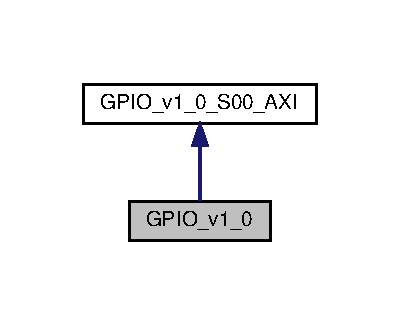
\includegraphics[width=192pt]{classGPIO__v1__0__inherit__graph}
\end{center}
\end{figure}


Collaboration diagram for G\+P\+I\+O\+\_\+v1\+\_\+0\+:\nopagebreak
\begin{figure}[H]
\begin{center}
\leavevmode
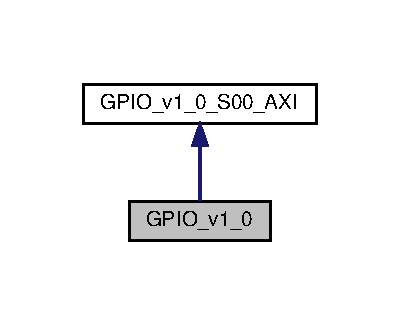
\includegraphics[width=192pt]{classGPIO__v1__0__coll__graph}
\end{center}
\end{figure}
\subsection*{Entities}
\begin{DoxyCompactItemize}
\item 
\hyperlink{classGPIO__v1__0_1_1arch__imp}{arch\+\_\+imp} architecture
\end{DoxyCompactItemize}
\subsection*{Libraries}
 \begin{DoxyCompactItemize}
\item 
\mbox{\Hypertarget{classGPIO__v1__0_a0a6af6eef40212dbaf130d57ce711256}\label{classGPIO__v1__0_a0a6af6eef40212dbaf130d57ce711256}} 
\hyperlink{classGPIO__v1__0_a0a6af6eef40212dbaf130d57ce711256}{ieee} 
\begin{DoxyCompactList}\small\item\em Viene utilizzata la libreria I\+E\+EE. \end{DoxyCompactList}\end{DoxyCompactItemize}
\subsection*{Use Clauses}
 \begin{DoxyCompactItemize}
\item 
\mbox{\Hypertarget{classGPIO__v1__0_acd03516902501cd1c7296a98e22c6fcb}\label{classGPIO__v1__0_acd03516902501cd1c7296a98e22c6fcb}} 
\hyperlink{classGPIO__v1__0_acd03516902501cd1c7296a98e22c6fcb}{std\+\_\+logic\+\_\+1164}   
\begin{DoxyCompactList}\small\item\em Sono utilizzati i segnali della standard logic. \end{DoxyCompactList}\item 
\mbox{\Hypertarget{classGPIO__v1__0_a2edc34402b573437d5f25fa90ba4013e}\label{classGPIO__v1__0_a2edc34402b573437d5f25fa90ba4013e}} 
\hyperlink{classGPIO__v1__0_a2edc34402b573437d5f25fa90ba4013e}{numeric\+\_\+std}   
\begin{DoxyCompactList}\small\item\em Vengono utilizzate le funzioni numeriche. \end{DoxyCompactList}\end{DoxyCompactItemize}
\subsection*{Generics}
 \begin{DoxyCompactItemize}
\item 
\mbox{\Hypertarget{classGPIO__v1__0_a16bbf9205afa677edb8a74dcd39ebb9f}\label{classGPIO__v1__0_a16bbf9205afa677edb8a74dcd39ebb9f}} 
\hyperlink{classGPIO__v1__0_a16bbf9205afa677edb8a74dcd39ebb9f}{width} {\bfseries {\bfseries \textcolor{vhdlchar}{integer}\textcolor{vhdlchar}{ }\textcolor{vhdlchar}{ }\textcolor{vhdlchar}{\+:}\textcolor{vhdlchar}{=}\textcolor{vhdlchar}{ }\textcolor{vhdlchar}{ } \textcolor{vhdldigit}{4} \textcolor{vhdlchar}{ }}}
\begin{DoxyCompactList}\small\item\em determina il numero di \hyperlink{structGPIO}{G\+P\+IO} da controllare \end{DoxyCompactList}\item 
\mbox{\Hypertarget{classGPIO__v1__0_afce7943994a4ddfa81f224225976a4c7}\label{classGPIO__v1__0_afce7943994a4ddfa81f224225976a4c7}} 
\hyperlink{classGPIO__v1__0_afce7943994a4ddfa81f224225976a4c7}{C\+\_\+\+S00\+\_\+\+A\+X\+I\+\_\+\+D\+A\+T\+A\+\_\+\+W\+I\+D\+TH} {\bfseries {\bfseries \textcolor{vhdlchar}{integer}\textcolor{vhdlchar}{ }\textcolor{vhdlchar}{ }\textcolor{vhdlchar}{\+:}\textcolor{vhdlchar}{=}\textcolor{vhdlchar}{ }\textcolor{vhdlchar}{ } \textcolor{vhdldigit}{32} \textcolor{vhdlchar}{ }}}
\item 
\mbox{\Hypertarget{classGPIO__v1__0_ab7787f274c76bb896ac98fdcfb570c65}\label{classGPIO__v1__0_ab7787f274c76bb896ac98fdcfb570c65}} 
\hyperlink{classGPIO__v1__0_ab7787f274c76bb896ac98fdcfb570c65}{C\+\_\+\+S00\+\_\+\+A\+X\+I\+\_\+\+A\+D\+D\+R\+\_\+\+W\+I\+D\+TH} {\bfseries {\bfseries \textcolor{vhdlchar}{integer}\textcolor{vhdlchar}{ }\textcolor{vhdlchar}{ }\textcolor{vhdlchar}{\+:}\textcolor{vhdlchar}{=}\textcolor{vhdlchar}{ }\textcolor{vhdlchar}{ } \textcolor{vhdldigit}{5} \textcolor{vhdlchar}{ }}}
\end{DoxyCompactItemize}
\subsection*{Ports}
 \begin{DoxyCompactItemize}
\item 
\mbox{\Hypertarget{classGPIO__v1__0_ac0744a550c27f11ab186fd7a1156a54e}\label{classGPIO__v1__0_ac0744a550c27f11ab186fd7a1156a54e}} 
\hyperlink{classGPIO__v1__0_ac0744a550c27f11ab186fd7a1156a54e}{pads}  {\bfseries {\bfseries \textcolor{vhdlchar}{inout}\textcolor{vhdlchar}{ }}} {\bfseries \textcolor{vhdlchar}{std\+\_\+logic\+\_\+vector}\textcolor{vhdlchar}{ }\textcolor{vhdlchar}{(}\textcolor{vhdlchar}{ }\textcolor{vhdlchar}{ }\textcolor{vhdlchar}{ }\textcolor{vhdlchar}{ }{\bfseries \hyperlink{classGPIO__v1__0_a16bbf9205afa677edb8a74dcd39ebb9f}{width}} \textcolor{vhdlchar}{-\/}\textcolor{vhdlchar}{ } \textcolor{vhdldigit}{1} \textcolor{vhdlchar}{ }\textcolor{vhdlchar}{downto}\textcolor{vhdlchar}{ }\textcolor{vhdlchar}{ } \textcolor{vhdldigit}{0} \textcolor{vhdlchar}{ }\textcolor{vhdlchar}{)}\textcolor{vhdlchar}{ }} 
\begin{DoxyCompactList}\small\item\em se \hyperlink{structGPIO}{G\+P\+IO} in modalità lettura mostra il valore letto, altrimenti forza un valore in uscita \end{DoxyCompactList}\item 
\mbox{\Hypertarget{classGPIO__v1__0_a5b78f3e3edfaf6e8ec79031b9e631e9d}\label{classGPIO__v1__0_a5b78f3e3edfaf6e8ec79031b9e631e9d}} 
\hyperlink{classGPIO__v1__0_a5b78f3e3edfaf6e8ec79031b9e631e9d}{interrupt}  {\bfseries {\bfseries \textcolor{vhdlchar}{out}\textcolor{vhdlchar}{ }}} {\bfseries \textcolor{vhdlchar}{std\+\_\+logic}\textcolor{vhdlchar}{ }} 
\begin{DoxyCompactList}\small\item\em segnale di interrupt \end{DoxyCompactList}\item 
\mbox{\Hypertarget{classGPIO__v1__0_a037f9e3df8559bfd59db37bcba9cb7a8}\label{classGPIO__v1__0_a037f9e3df8559bfd59db37bcba9cb7a8}} 
\hyperlink{classGPIO__v1__0_a037f9e3df8559bfd59db37bcba9cb7a8}{s00\+\_\+axi\+\_\+aclk}  {\bfseries {\bfseries \textcolor{vhdlchar}{in}\textcolor{vhdlchar}{ }}} {\bfseries \textcolor{vhdlchar}{std\+\_\+logic}\textcolor{vhdlchar}{ }} 
\item 
\mbox{\Hypertarget{classGPIO__v1__0_a8249c106fbd80196dcad2666c9f0b3fc}\label{classGPIO__v1__0_a8249c106fbd80196dcad2666c9f0b3fc}} 
\hyperlink{classGPIO__v1__0_a8249c106fbd80196dcad2666c9f0b3fc}{s00\+\_\+axi\+\_\+aresetn}  {\bfseries {\bfseries \textcolor{vhdlchar}{in}\textcolor{vhdlchar}{ }}} {\bfseries \textcolor{vhdlchar}{std\+\_\+logic}\textcolor{vhdlchar}{ }} 
\item 
\mbox{\Hypertarget{classGPIO__v1__0_a9fe80d3cc7f862afb670536e4e05dbeb}\label{classGPIO__v1__0_a9fe80d3cc7f862afb670536e4e05dbeb}} 
\hyperlink{classGPIO__v1__0_a9fe80d3cc7f862afb670536e4e05dbeb}{s00\+\_\+axi\+\_\+awaddr}  {\bfseries {\bfseries \textcolor{vhdlchar}{in}\textcolor{vhdlchar}{ }}} {\bfseries \textcolor{vhdlchar}{std\+\_\+logic\+\_\+vector}\textcolor{vhdlchar}{ }\textcolor{vhdlchar}{(}\textcolor{vhdlchar}{ }\textcolor{vhdlchar}{ }\textcolor{vhdlchar}{ }\textcolor{vhdlchar}{ }\textcolor{vhdlchar}{C\+\_\+\+S00\+\_\+\+A\+X\+I\+\_\+\+A\+D\+D\+R\+\_\+\+W\+I\+D\+TH}\textcolor{vhdlchar}{-\/}\textcolor{vhdlchar}{ } \textcolor{vhdldigit}{1} \textcolor{vhdlchar}{ }\textcolor{vhdlchar}{downto}\textcolor{vhdlchar}{ }\textcolor{vhdlchar}{ } \textcolor{vhdldigit}{0} \textcolor{vhdlchar}{ }\textcolor{vhdlchar}{)}\textcolor{vhdlchar}{ }} 
\item 
\mbox{\Hypertarget{classGPIO__v1__0_a719659c1addef5432978cc949d9e10ed}\label{classGPIO__v1__0_a719659c1addef5432978cc949d9e10ed}} 
\hyperlink{classGPIO__v1__0_a719659c1addef5432978cc949d9e10ed}{s00\+\_\+axi\+\_\+awprot}  {\bfseries {\bfseries \textcolor{vhdlchar}{in}\textcolor{vhdlchar}{ }}} {\bfseries \textcolor{vhdlchar}{std\+\_\+logic\+\_\+vector}\textcolor{vhdlchar}{ }\textcolor{vhdlchar}{(}\textcolor{vhdlchar}{ }\textcolor{vhdlchar}{ } \textcolor{vhdldigit}{2} \textcolor{vhdlchar}{ }\textcolor{vhdlchar}{downto}\textcolor{vhdlchar}{ }\textcolor{vhdlchar}{ } \textcolor{vhdldigit}{0} \textcolor{vhdlchar}{ }\textcolor{vhdlchar}{)}\textcolor{vhdlchar}{ }} 
\item 
\mbox{\Hypertarget{classGPIO__v1__0_a45aa02a72ae1a8389346d47173c60ed0}\label{classGPIO__v1__0_a45aa02a72ae1a8389346d47173c60ed0}} 
\hyperlink{classGPIO__v1__0_a45aa02a72ae1a8389346d47173c60ed0}{s00\+\_\+axi\+\_\+awvalid}  {\bfseries {\bfseries \textcolor{vhdlchar}{in}\textcolor{vhdlchar}{ }}} {\bfseries \textcolor{vhdlchar}{std\+\_\+logic}\textcolor{vhdlchar}{ }} 
\item 
\mbox{\Hypertarget{classGPIO__v1__0_ad0a1f71502d91a45dbc6c365f85c6566}\label{classGPIO__v1__0_ad0a1f71502d91a45dbc6c365f85c6566}} 
\hyperlink{classGPIO__v1__0_ad0a1f71502d91a45dbc6c365f85c6566}{s00\+\_\+axi\+\_\+awready}  {\bfseries {\bfseries \textcolor{vhdlchar}{out}\textcolor{vhdlchar}{ }}} {\bfseries \textcolor{vhdlchar}{std\+\_\+logic}\textcolor{vhdlchar}{ }} 
\item 
\mbox{\Hypertarget{classGPIO__v1__0_ae2b15b55ee463fd9dd030ee29db6bb17}\label{classGPIO__v1__0_ae2b15b55ee463fd9dd030ee29db6bb17}} 
\hyperlink{classGPIO__v1__0_ae2b15b55ee463fd9dd030ee29db6bb17}{s00\+\_\+axi\+\_\+wdata}  {\bfseries {\bfseries \textcolor{vhdlchar}{in}\textcolor{vhdlchar}{ }}} {\bfseries \textcolor{vhdlchar}{std\+\_\+logic\+\_\+vector}\textcolor{vhdlchar}{ }\textcolor{vhdlchar}{(}\textcolor{vhdlchar}{ }\textcolor{vhdlchar}{ }\textcolor{vhdlchar}{ }\textcolor{vhdlchar}{ }\textcolor{vhdlchar}{C\+\_\+\+S00\+\_\+\+A\+X\+I\+\_\+\+D\+A\+T\+A\+\_\+\+W\+I\+D\+TH}\textcolor{vhdlchar}{-\/}\textcolor{vhdlchar}{ } \textcolor{vhdldigit}{1} \textcolor{vhdlchar}{ }\textcolor{vhdlchar}{downto}\textcolor{vhdlchar}{ }\textcolor{vhdlchar}{ } \textcolor{vhdldigit}{0} \textcolor{vhdlchar}{ }\textcolor{vhdlchar}{)}\textcolor{vhdlchar}{ }} 
\item 
\mbox{\Hypertarget{classGPIO__v1__0_a120924bc3fd5fd10ec0f96e19c3f4904}\label{classGPIO__v1__0_a120924bc3fd5fd10ec0f96e19c3f4904}} 
\hyperlink{classGPIO__v1__0_a120924bc3fd5fd10ec0f96e19c3f4904}{s00\+\_\+axi\+\_\+wstrb}  {\bfseries {\bfseries \textcolor{vhdlchar}{in}\textcolor{vhdlchar}{ }}} {\bfseries \textcolor{vhdlchar}{std\+\_\+logic\+\_\+vector}\textcolor{vhdlchar}{ }\textcolor{vhdlchar}{(}\textcolor{vhdlchar}{ }\textcolor{vhdlchar}{(}\textcolor{vhdlchar}{ }\textcolor{vhdlchar}{ }\textcolor{vhdlchar}{ }\textcolor{vhdlchar}{ }\textcolor{vhdlchar}{C\+\_\+\+S00\+\_\+\+A\+X\+I\+\_\+\+D\+A\+T\+A\+\_\+\+W\+I\+D\+TH}\textcolor{vhdlchar}{/}\textcolor{vhdlchar}{ } \textcolor{vhdldigit}{8} \textcolor{vhdlchar}{ }\textcolor{vhdlchar}{)}\textcolor{vhdlchar}{ }\textcolor{vhdlchar}{-\/}\textcolor{vhdlchar}{ } \textcolor{vhdldigit}{1} \textcolor{vhdlchar}{ }\textcolor{vhdlchar}{downto}\textcolor{vhdlchar}{ }\textcolor{vhdlchar}{ } \textcolor{vhdldigit}{0} \textcolor{vhdlchar}{ }\textcolor{vhdlchar}{)}\textcolor{vhdlchar}{ }} 
\item 
\mbox{\Hypertarget{classGPIO__v1__0_a24e90907193647007d2947353740114d}\label{classGPIO__v1__0_a24e90907193647007d2947353740114d}} 
\hyperlink{classGPIO__v1__0_a24e90907193647007d2947353740114d}{s00\+\_\+axi\+\_\+wvalid}  {\bfseries {\bfseries \textcolor{vhdlchar}{in}\textcolor{vhdlchar}{ }}} {\bfseries \textcolor{vhdlchar}{std\+\_\+logic}\textcolor{vhdlchar}{ }} 
\item 
\mbox{\Hypertarget{classGPIO__v1__0_a3fc60abc0cfbfa90003a83bffdd476c4}\label{classGPIO__v1__0_a3fc60abc0cfbfa90003a83bffdd476c4}} 
\hyperlink{classGPIO__v1__0_a3fc60abc0cfbfa90003a83bffdd476c4}{s00\+\_\+axi\+\_\+wready}  {\bfseries {\bfseries \textcolor{vhdlchar}{out}\textcolor{vhdlchar}{ }}} {\bfseries \textcolor{vhdlchar}{std\+\_\+logic}\textcolor{vhdlchar}{ }} 
\item 
\mbox{\Hypertarget{classGPIO__v1__0_af8799be946d3f5354263e7deb15f94f1}\label{classGPIO__v1__0_af8799be946d3f5354263e7deb15f94f1}} 
\hyperlink{classGPIO__v1__0_af8799be946d3f5354263e7deb15f94f1}{s00\+\_\+axi\+\_\+bresp}  {\bfseries {\bfseries \textcolor{vhdlchar}{out}\textcolor{vhdlchar}{ }}} {\bfseries \textcolor{vhdlchar}{std\+\_\+logic\+\_\+vector}\textcolor{vhdlchar}{ }\textcolor{vhdlchar}{(}\textcolor{vhdlchar}{ }\textcolor{vhdlchar}{ } \textcolor{vhdldigit}{1} \textcolor{vhdlchar}{ }\textcolor{vhdlchar}{downto}\textcolor{vhdlchar}{ }\textcolor{vhdlchar}{ } \textcolor{vhdldigit}{0} \textcolor{vhdlchar}{ }\textcolor{vhdlchar}{)}\textcolor{vhdlchar}{ }} 
\item 
\mbox{\Hypertarget{classGPIO__v1__0_a5110b7dd4fb9548a2aab88f50dbe1d5e}\label{classGPIO__v1__0_a5110b7dd4fb9548a2aab88f50dbe1d5e}} 
\hyperlink{classGPIO__v1__0_a5110b7dd4fb9548a2aab88f50dbe1d5e}{s00\+\_\+axi\+\_\+bvalid}  {\bfseries {\bfseries \textcolor{vhdlchar}{out}\textcolor{vhdlchar}{ }}} {\bfseries \textcolor{vhdlchar}{std\+\_\+logic}\textcolor{vhdlchar}{ }} 
\item 
\mbox{\Hypertarget{classGPIO__v1__0_a1ef2019b0613bc23d4829eeeb24eb98d}\label{classGPIO__v1__0_a1ef2019b0613bc23d4829eeeb24eb98d}} 
\hyperlink{classGPIO__v1__0_a1ef2019b0613bc23d4829eeeb24eb98d}{s00\+\_\+axi\+\_\+bready}  {\bfseries {\bfseries \textcolor{vhdlchar}{in}\textcolor{vhdlchar}{ }}} {\bfseries \textcolor{vhdlchar}{std\+\_\+logic}\textcolor{vhdlchar}{ }} 
\item 
\mbox{\Hypertarget{classGPIO__v1__0_af70a86336cd6505064e45b69f4623939}\label{classGPIO__v1__0_af70a86336cd6505064e45b69f4623939}} 
\hyperlink{classGPIO__v1__0_af70a86336cd6505064e45b69f4623939}{s00\+\_\+axi\+\_\+araddr}  {\bfseries {\bfseries \textcolor{vhdlchar}{in}\textcolor{vhdlchar}{ }}} {\bfseries \textcolor{vhdlchar}{std\+\_\+logic\+\_\+vector}\textcolor{vhdlchar}{ }\textcolor{vhdlchar}{(}\textcolor{vhdlchar}{ }\textcolor{vhdlchar}{ }\textcolor{vhdlchar}{ }\textcolor{vhdlchar}{ }\textcolor{vhdlchar}{C\+\_\+\+S00\+\_\+\+A\+X\+I\+\_\+\+A\+D\+D\+R\+\_\+\+W\+I\+D\+TH}\textcolor{vhdlchar}{-\/}\textcolor{vhdlchar}{ } \textcolor{vhdldigit}{1} \textcolor{vhdlchar}{ }\textcolor{vhdlchar}{downto}\textcolor{vhdlchar}{ }\textcolor{vhdlchar}{ } \textcolor{vhdldigit}{0} \textcolor{vhdlchar}{ }\textcolor{vhdlchar}{)}\textcolor{vhdlchar}{ }} 
\item 
\mbox{\Hypertarget{classGPIO__v1__0_adc648df07895bf808b8c721e1dc6811b}\label{classGPIO__v1__0_adc648df07895bf808b8c721e1dc6811b}} 
\hyperlink{classGPIO__v1__0_adc648df07895bf808b8c721e1dc6811b}{s00\+\_\+axi\+\_\+arprot}  {\bfseries {\bfseries \textcolor{vhdlchar}{in}\textcolor{vhdlchar}{ }}} {\bfseries \textcolor{vhdlchar}{std\+\_\+logic\+\_\+vector}\textcolor{vhdlchar}{ }\textcolor{vhdlchar}{(}\textcolor{vhdlchar}{ }\textcolor{vhdlchar}{ } \textcolor{vhdldigit}{2} \textcolor{vhdlchar}{ }\textcolor{vhdlchar}{downto}\textcolor{vhdlchar}{ }\textcolor{vhdlchar}{ } \textcolor{vhdldigit}{0} \textcolor{vhdlchar}{ }\textcolor{vhdlchar}{)}\textcolor{vhdlchar}{ }} 
\item 
\mbox{\Hypertarget{classGPIO__v1__0_a94b78b2ae3cd13860f15afbdfb199e44}\label{classGPIO__v1__0_a94b78b2ae3cd13860f15afbdfb199e44}} 
\hyperlink{classGPIO__v1__0_a94b78b2ae3cd13860f15afbdfb199e44}{s00\+\_\+axi\+\_\+arvalid}  {\bfseries {\bfseries \textcolor{vhdlchar}{in}\textcolor{vhdlchar}{ }}} {\bfseries \textcolor{vhdlchar}{std\+\_\+logic}\textcolor{vhdlchar}{ }} 
\item 
\mbox{\Hypertarget{classGPIO__v1__0_ad35bd95f3352ff8dbdaea55205a98e53}\label{classGPIO__v1__0_ad35bd95f3352ff8dbdaea55205a98e53}} 
\hyperlink{classGPIO__v1__0_ad35bd95f3352ff8dbdaea55205a98e53}{s00\+\_\+axi\+\_\+arready}  {\bfseries {\bfseries \textcolor{vhdlchar}{out}\textcolor{vhdlchar}{ }}} {\bfseries \textcolor{vhdlchar}{std\+\_\+logic}\textcolor{vhdlchar}{ }} 
\item 
\mbox{\Hypertarget{classGPIO__v1__0_ad2655fadb987e0487c428aca187b55d0}\label{classGPIO__v1__0_ad2655fadb987e0487c428aca187b55d0}} 
\hyperlink{classGPIO__v1__0_ad2655fadb987e0487c428aca187b55d0}{s00\+\_\+axi\+\_\+rdata}  {\bfseries {\bfseries \textcolor{vhdlchar}{out}\textcolor{vhdlchar}{ }}} {\bfseries \textcolor{vhdlchar}{std\+\_\+logic\+\_\+vector}\textcolor{vhdlchar}{ }\textcolor{vhdlchar}{(}\textcolor{vhdlchar}{ }\textcolor{vhdlchar}{ }\textcolor{vhdlchar}{ }\textcolor{vhdlchar}{ }\textcolor{vhdlchar}{C\+\_\+\+S00\+\_\+\+A\+X\+I\+\_\+\+D\+A\+T\+A\+\_\+\+W\+I\+D\+TH}\textcolor{vhdlchar}{-\/}\textcolor{vhdlchar}{ } \textcolor{vhdldigit}{1} \textcolor{vhdlchar}{ }\textcolor{vhdlchar}{downto}\textcolor{vhdlchar}{ }\textcolor{vhdlchar}{ } \textcolor{vhdldigit}{0} \textcolor{vhdlchar}{ }\textcolor{vhdlchar}{)}\textcolor{vhdlchar}{ }} 
\item 
\mbox{\Hypertarget{classGPIO__v1__0_a1acee955f50f71e5595a03c6ca301cf0}\label{classGPIO__v1__0_a1acee955f50f71e5595a03c6ca301cf0}} 
\hyperlink{classGPIO__v1__0_a1acee955f50f71e5595a03c6ca301cf0}{s00\+\_\+axi\+\_\+rresp}  {\bfseries {\bfseries \textcolor{vhdlchar}{out}\textcolor{vhdlchar}{ }}} {\bfseries \textcolor{vhdlchar}{std\+\_\+logic\+\_\+vector}\textcolor{vhdlchar}{ }\textcolor{vhdlchar}{(}\textcolor{vhdlchar}{ }\textcolor{vhdlchar}{ } \textcolor{vhdldigit}{1} \textcolor{vhdlchar}{ }\textcolor{vhdlchar}{downto}\textcolor{vhdlchar}{ }\textcolor{vhdlchar}{ } \textcolor{vhdldigit}{0} \textcolor{vhdlchar}{ }\textcolor{vhdlchar}{)}\textcolor{vhdlchar}{ }} 
\item 
\mbox{\Hypertarget{classGPIO__v1__0_af180911f7eb262e530e26865bc97aa0b}\label{classGPIO__v1__0_af180911f7eb262e530e26865bc97aa0b}} 
\hyperlink{classGPIO__v1__0_af180911f7eb262e530e26865bc97aa0b}{s00\+\_\+axi\+\_\+rvalid}  {\bfseries {\bfseries \textcolor{vhdlchar}{out}\textcolor{vhdlchar}{ }}} {\bfseries \textcolor{vhdlchar}{std\+\_\+logic}\textcolor{vhdlchar}{ }} 
\item 
\mbox{\Hypertarget{classGPIO__v1__0_a8b82eb165d7024f6c7b25646f6ebdd4d}\label{classGPIO__v1__0_a8b82eb165d7024f6c7b25646f6ebdd4d}} 
\hyperlink{classGPIO__v1__0_a8b82eb165d7024f6c7b25646f6ebdd4d}{s00\+\_\+axi\+\_\+rready}  {\bfseries {\bfseries \textcolor{vhdlchar}{in}\textcolor{vhdlchar}{ }}} {\bfseries \textcolor{vhdlchar}{std\+\_\+logic}\textcolor{vhdlchar}{ }} 
\end{DoxyCompactItemize}


The documentation for this class was generated from the following file\+:\begin{DoxyCompactItemize}
\item 
/media/saverio/\+O\+S/\+Users/\+Saverio/\+Desktop/\+S\+E/git/codici\+\_\+da\+\_\+mandare/\+F\+P\+G\+A/\+G\+P\+I\+O/\+Hardware/\+G\+P\+I\+O\+\_\+1.\+0/hdl/\hyperlink{GPIO__v1__0_8vhd}{G\+P\+I\+O\+\_\+v1\+\_\+0.\+vhd}\end{DoxyCompactItemize}

\hypertarget{classGPIO__v1__0__S00__AXI}{}\section{G\+P\+I\+O\+\_\+v1\+\_\+0\+\_\+\+S00\+\_\+\+A\+XI Entity Reference}
\label{classGPIO__v1__0__S00__AXI}\index{G\+P\+I\+O\+\_\+v1\+\_\+0\+\_\+\+S00\+\_\+\+A\+XI@{G\+P\+I\+O\+\_\+v1\+\_\+0\+\_\+\+S00\+\_\+\+A\+XI}}


Inheritance diagram for G\+P\+I\+O\+\_\+v1\+\_\+0\+\_\+\+S00\+\_\+\+A\+XI\+:\nopagebreak
\begin{figure}[H]
\begin{center}
\leavevmode
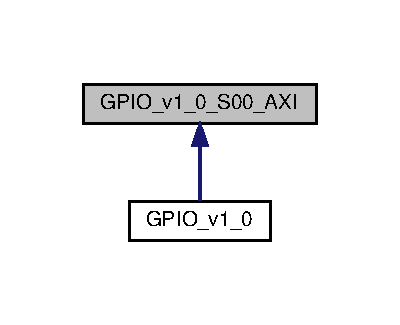
\includegraphics[width=192pt]{classGPIO__v1__0__S00__AXI__inherit__graph}
\end{center}
\end{figure}
\subsection*{Entities}
\begin{DoxyCompactItemize}
\item 
\hyperlink{classGPIO__v1__0__S00__AXI_1_1arch__imp}{arch\+\_\+imp} architecture
\end{DoxyCompactItemize}
\subsection*{Libraries}
 \begin{DoxyCompactItemize}
\item 
\mbox{\Hypertarget{classGPIO__v1__0__S00__AXI_a0a6af6eef40212dbaf130d57ce711256}\label{classGPIO__v1__0__S00__AXI_a0a6af6eef40212dbaf130d57ce711256}} 
\hyperlink{classGPIO__v1__0__S00__AXI_a0a6af6eef40212dbaf130d57ce711256}{ieee} 
\begin{DoxyCompactList}\small\item\em Viene utilizzato la libreria I\+E\+EE. \end{DoxyCompactList}\end{DoxyCompactItemize}
\subsection*{Use Clauses}
 \begin{DoxyCompactItemize}
\item 
\mbox{\Hypertarget{classGPIO__v1__0__S00__AXI_acd03516902501cd1c7296a98e22c6fcb}\label{classGPIO__v1__0__S00__AXI_acd03516902501cd1c7296a98e22c6fcb}} 
\hyperlink{classGPIO__v1__0__S00__AXI_acd03516902501cd1c7296a98e22c6fcb}{std\+\_\+logic\+\_\+1164}   
\begin{DoxyCompactList}\small\item\em Sono utilizzati i segnali della standard logic. \end{DoxyCompactList}\item 
\mbox{\Hypertarget{classGPIO__v1__0__S00__AXI_a2edc34402b573437d5f25fa90ba4013e}\label{classGPIO__v1__0__S00__AXI_a2edc34402b573437d5f25fa90ba4013e}} 
\hyperlink{classGPIO__v1__0__S00__AXI_a2edc34402b573437d5f25fa90ba4013e}{numeric\+\_\+std}   
\begin{DoxyCompactList}\small\item\em Vengono utilizzate le funzioni numeriche. \end{DoxyCompactList}\item 
\mbox{\Hypertarget{classGPIO__v1__0__S00__AXI_acb2d98d781f19c8f5f4109576ec45502}\label{classGPIO__v1__0__S00__AXI_acb2d98d781f19c8f5f4109576ec45502}} 
\hyperlink{classGPIO__v1__0__S00__AXI_acb2d98d781f19c8f5f4109576ec45502}{std\+\_\+logic\+\_\+misc}   
\begin{DoxyCompactList}\small\item\em Viene utilizzata la libreria misc di utility. \end{DoxyCompactList}\end{DoxyCompactItemize}
\subsection*{Generics}
 \begin{DoxyCompactItemize}
\item 
\mbox{\Hypertarget{classGPIO__v1__0__S00__AXI_a16bbf9205afa677edb8a74dcd39ebb9f}\label{classGPIO__v1__0__S00__AXI_a16bbf9205afa677edb8a74dcd39ebb9f}} 
\hyperlink{classGPIO__v1__0__S00__AXI_a16bbf9205afa677edb8a74dcd39ebb9f}{width} {\bfseries {\bfseries \textcolor{vhdlchar}{integer}\textcolor{vhdlchar}{ }\textcolor{vhdlchar}{ }\textcolor{vhdlchar}{\+:}\textcolor{vhdlchar}{=}\textcolor{vhdlchar}{ }\textcolor{vhdlchar}{ } \textcolor{vhdldigit}{4} \textcolor{vhdlchar}{ }}}
\begin{DoxyCompactList}\small\item\em determina il numero di \hyperlink{structGPIO}{G\+P\+IO} da controllare \end{DoxyCompactList}\item 
\mbox{\Hypertarget{classGPIO__v1__0__S00__AXI_a0fad312acd1f302ce7de30c5658df0bd}\label{classGPIO__v1__0__S00__AXI_a0fad312acd1f302ce7de30c5658df0bd}} 
\hyperlink{classGPIO__v1__0__S00__AXI_a0fad312acd1f302ce7de30c5658df0bd}{C\+\_\+\+S\+\_\+\+A\+X\+I\+\_\+\+D\+A\+T\+A\+\_\+\+W\+I\+D\+TH} {\bfseries {\bfseries \textcolor{vhdlchar}{integer}\textcolor{vhdlchar}{ }\textcolor{vhdlchar}{ }\textcolor{vhdlchar}{\+:}\textcolor{vhdlchar}{=}\textcolor{vhdlchar}{ }\textcolor{vhdlchar}{ } \textcolor{vhdldigit}{32} \textcolor{vhdlchar}{ }}}
\item 
\mbox{\Hypertarget{classGPIO__v1__0__S00__AXI_a9abff2eaa069440f3b7d9e9937d5ee8e}\label{classGPIO__v1__0__S00__AXI_a9abff2eaa069440f3b7d9e9937d5ee8e}} 
\hyperlink{classGPIO__v1__0__S00__AXI_a9abff2eaa069440f3b7d9e9937d5ee8e}{C\+\_\+\+S\+\_\+\+A\+X\+I\+\_\+\+A\+D\+D\+R\+\_\+\+W\+I\+D\+TH} {\bfseries {\bfseries \textcolor{vhdlchar}{integer}\textcolor{vhdlchar}{ }\textcolor{vhdlchar}{ }\textcolor{vhdlchar}{\+:}\textcolor{vhdlchar}{=}\textcolor{vhdlchar}{ }\textcolor{vhdlchar}{ } \textcolor{vhdldigit}{5} \textcolor{vhdlchar}{ }}}
\end{DoxyCompactItemize}
\subsection*{Ports}
 \begin{DoxyCompactItemize}
\item 
\mbox{\Hypertarget{classGPIO__v1__0__S00__AXI_ac0744a550c27f11ab186fd7a1156a54e}\label{classGPIO__v1__0__S00__AXI_ac0744a550c27f11ab186fd7a1156a54e}} 
\hyperlink{classGPIO__v1__0__S00__AXI_ac0744a550c27f11ab186fd7a1156a54e}{pads}  {\bfseries {\bfseries \textcolor{vhdlchar}{inout}\textcolor{vhdlchar}{ }}} {\bfseries \textcolor{vhdlchar}{std\+\_\+logic\+\_\+vector}\textcolor{vhdlchar}{ }\textcolor{vhdlchar}{(}\textcolor{vhdlchar}{ }\textcolor{vhdlchar}{ }\textcolor{vhdlchar}{ }\textcolor{vhdlchar}{ }{\bfseries \hyperlink{classGPIO__v1__0__S00__AXI_a16bbf9205afa677edb8a74dcd39ebb9f}{width}} \textcolor{vhdlchar}{-\/}\textcolor{vhdlchar}{ } \textcolor{vhdldigit}{1} \textcolor{vhdlchar}{ }\textcolor{vhdlchar}{downto}\textcolor{vhdlchar}{ }\textcolor{vhdlchar}{ } \textcolor{vhdldigit}{0} \textcolor{vhdlchar}{ }\textcolor{vhdlchar}{)}\textcolor{vhdlchar}{ }} 
\begin{DoxyCompactList}\small\item\em se \hyperlink{structGPIO}{G\+P\+IO} in modalità lettura mostra il valore letto, altrimenti forza un valore in uscita \end{DoxyCompactList}\item 
\mbox{\Hypertarget{classGPIO__v1__0__S00__AXI_a5b78f3e3edfaf6e8ec79031b9e631e9d}\label{classGPIO__v1__0__S00__AXI_a5b78f3e3edfaf6e8ec79031b9e631e9d}} 
\hyperlink{classGPIO__v1__0__S00__AXI_a5b78f3e3edfaf6e8ec79031b9e631e9d}{interrupt}  {\bfseries {\bfseries \textcolor{vhdlchar}{out}\textcolor{vhdlchar}{ }}} {\bfseries \textcolor{vhdlchar}{std\+\_\+logic}\textcolor{vhdlchar}{ }} 
\begin{DoxyCompactList}\small\item\em segnale di interrupt \end{DoxyCompactList}\item 
\mbox{\Hypertarget{classGPIO__v1__0__S00__AXI_a3f54d782a88290bdaa6baffd7cd84ab4}\label{classGPIO__v1__0__S00__AXI_a3f54d782a88290bdaa6baffd7cd84ab4}} 
\hyperlink{classGPIO__v1__0__S00__AXI_a3f54d782a88290bdaa6baffd7cd84ab4}{S\+\_\+\+A\+X\+I\+\_\+\+A\+C\+LK}  {\bfseries {\bfseries \textcolor{vhdlchar}{in}\textcolor{vhdlchar}{ }}} {\bfseries \textcolor{vhdlchar}{std\+\_\+logic}\textcolor{vhdlchar}{ }} 
\item 
\mbox{\Hypertarget{classGPIO__v1__0__S00__AXI_a089b396e17dee353ccc7d5389dda5532}\label{classGPIO__v1__0__S00__AXI_a089b396e17dee353ccc7d5389dda5532}} 
\hyperlink{classGPIO__v1__0__S00__AXI_a089b396e17dee353ccc7d5389dda5532}{S\+\_\+\+A\+X\+I\+\_\+\+A\+R\+E\+S\+E\+TN}  {\bfseries {\bfseries \textcolor{vhdlchar}{in}\textcolor{vhdlchar}{ }}} {\bfseries \textcolor{vhdlchar}{std\+\_\+logic}\textcolor{vhdlchar}{ }} 
\item 
\mbox{\Hypertarget{classGPIO__v1__0__S00__AXI_a61cc7b190ba9d540e56941330e4a0883}\label{classGPIO__v1__0__S00__AXI_a61cc7b190ba9d540e56941330e4a0883}} 
\hyperlink{classGPIO__v1__0__S00__AXI_a61cc7b190ba9d540e56941330e4a0883}{S\+\_\+\+A\+X\+I\+\_\+\+A\+W\+A\+D\+DR}  {\bfseries {\bfseries \textcolor{vhdlchar}{in}\textcolor{vhdlchar}{ }}} {\bfseries \textcolor{vhdlchar}{std\+\_\+logic\+\_\+vector}\textcolor{vhdlchar}{ }\textcolor{vhdlchar}{(}\textcolor{vhdlchar}{ }\textcolor{vhdlchar}{ }\textcolor{vhdlchar}{ }\textcolor{vhdlchar}{ }\textcolor{vhdlchar}{C\+\_\+\+S\+\_\+\+A\+X\+I\+\_\+\+A\+D\+D\+R\+\_\+\+W\+I\+D\+TH}\textcolor{vhdlchar}{-\/}\textcolor{vhdlchar}{ } \textcolor{vhdldigit}{1} \textcolor{vhdlchar}{ }\textcolor{vhdlchar}{downto}\textcolor{vhdlchar}{ }\textcolor{vhdlchar}{ } \textcolor{vhdldigit}{0} \textcolor{vhdlchar}{ }\textcolor{vhdlchar}{)}\textcolor{vhdlchar}{ }} 
\item 
\mbox{\Hypertarget{classGPIO__v1__0__S00__AXI_a459abcd98567ad24261377eed899593a}\label{classGPIO__v1__0__S00__AXI_a459abcd98567ad24261377eed899593a}} 
\hyperlink{classGPIO__v1__0__S00__AXI_a459abcd98567ad24261377eed899593a}{S\+\_\+\+A\+X\+I\+\_\+\+A\+W\+P\+R\+OT}  {\bfseries {\bfseries \textcolor{vhdlchar}{in}\textcolor{vhdlchar}{ }}} {\bfseries \textcolor{vhdlchar}{std\+\_\+logic\+\_\+vector}\textcolor{vhdlchar}{ }\textcolor{vhdlchar}{(}\textcolor{vhdlchar}{ }\textcolor{vhdlchar}{ } \textcolor{vhdldigit}{2} \textcolor{vhdlchar}{ }\textcolor{vhdlchar}{downto}\textcolor{vhdlchar}{ }\textcolor{vhdlchar}{ } \textcolor{vhdldigit}{0} \textcolor{vhdlchar}{ }\textcolor{vhdlchar}{)}\textcolor{vhdlchar}{ }} 
\item 
\mbox{\Hypertarget{classGPIO__v1__0__S00__AXI_af1f1cbf67bf647ba58353c261719a3a0}\label{classGPIO__v1__0__S00__AXI_af1f1cbf67bf647ba58353c261719a3a0}} 
\hyperlink{classGPIO__v1__0__S00__AXI_af1f1cbf67bf647ba58353c261719a3a0}{S\+\_\+\+A\+X\+I\+\_\+\+A\+W\+V\+A\+L\+ID}  {\bfseries {\bfseries \textcolor{vhdlchar}{in}\textcolor{vhdlchar}{ }}} {\bfseries \textcolor{vhdlchar}{std\+\_\+logic}\textcolor{vhdlchar}{ }} 
\item 
\mbox{\Hypertarget{classGPIO__v1__0__S00__AXI_ac04aab5cc834e762e893e061016921c6}\label{classGPIO__v1__0__S00__AXI_ac04aab5cc834e762e893e061016921c6}} 
\hyperlink{classGPIO__v1__0__S00__AXI_ac04aab5cc834e762e893e061016921c6}{S\+\_\+\+A\+X\+I\+\_\+\+A\+W\+R\+E\+A\+DY}  {\bfseries {\bfseries \textcolor{vhdlchar}{out}\textcolor{vhdlchar}{ }}} {\bfseries \textcolor{vhdlchar}{std\+\_\+logic}\textcolor{vhdlchar}{ }} 
\item 
\mbox{\Hypertarget{classGPIO__v1__0__S00__AXI_a292e5db13719faf3a8b3aab091773467}\label{classGPIO__v1__0__S00__AXI_a292e5db13719faf3a8b3aab091773467}} 
\hyperlink{classGPIO__v1__0__S00__AXI_a292e5db13719faf3a8b3aab091773467}{S\+\_\+\+A\+X\+I\+\_\+\+W\+D\+A\+TA}  {\bfseries {\bfseries \textcolor{vhdlchar}{in}\textcolor{vhdlchar}{ }}} {\bfseries \textcolor{vhdlchar}{std\+\_\+logic\+\_\+vector}\textcolor{vhdlchar}{ }\textcolor{vhdlchar}{(}\textcolor{vhdlchar}{ }\textcolor{vhdlchar}{ }\textcolor{vhdlchar}{ }\textcolor{vhdlchar}{ }\textcolor{vhdlchar}{C\+\_\+\+S\+\_\+\+A\+X\+I\+\_\+\+D\+A\+T\+A\+\_\+\+W\+I\+D\+TH}\textcolor{vhdlchar}{-\/}\textcolor{vhdlchar}{ } \textcolor{vhdldigit}{1} \textcolor{vhdlchar}{ }\textcolor{vhdlchar}{downto}\textcolor{vhdlchar}{ }\textcolor{vhdlchar}{ } \textcolor{vhdldigit}{0} \textcolor{vhdlchar}{ }\textcolor{vhdlchar}{)}\textcolor{vhdlchar}{ }} 
\item 
\mbox{\Hypertarget{classGPIO__v1__0__S00__AXI_accd8e04b79540b57ab15fee1cb6c04f5}\label{classGPIO__v1__0__S00__AXI_accd8e04b79540b57ab15fee1cb6c04f5}} 
\hyperlink{classGPIO__v1__0__S00__AXI_accd8e04b79540b57ab15fee1cb6c04f5}{S\+\_\+\+A\+X\+I\+\_\+\+W\+S\+T\+RB}  {\bfseries {\bfseries \textcolor{vhdlchar}{in}\textcolor{vhdlchar}{ }}} {\bfseries \textcolor{vhdlchar}{std\+\_\+logic\+\_\+vector}\textcolor{vhdlchar}{ }\textcolor{vhdlchar}{(}\textcolor{vhdlchar}{ }\textcolor{vhdlchar}{(}\textcolor{vhdlchar}{ }\textcolor{vhdlchar}{ }\textcolor{vhdlchar}{ }\textcolor{vhdlchar}{ }\textcolor{vhdlchar}{C\+\_\+\+S\+\_\+\+A\+X\+I\+\_\+\+D\+A\+T\+A\+\_\+\+W\+I\+D\+TH}\textcolor{vhdlchar}{/}\textcolor{vhdlchar}{ } \textcolor{vhdldigit}{8} \textcolor{vhdlchar}{ }\textcolor{vhdlchar}{)}\textcolor{vhdlchar}{ }\textcolor{vhdlchar}{-\/}\textcolor{vhdlchar}{ } \textcolor{vhdldigit}{1} \textcolor{vhdlchar}{ }\textcolor{vhdlchar}{downto}\textcolor{vhdlchar}{ }\textcolor{vhdlchar}{ } \textcolor{vhdldigit}{0} \textcolor{vhdlchar}{ }\textcolor{vhdlchar}{)}\textcolor{vhdlchar}{ }} 
\item 
\mbox{\Hypertarget{classGPIO__v1__0__S00__AXI_a60bd882e2de781af9a7c6c3d494225d5}\label{classGPIO__v1__0__S00__AXI_a60bd882e2de781af9a7c6c3d494225d5}} 
\hyperlink{classGPIO__v1__0__S00__AXI_a60bd882e2de781af9a7c6c3d494225d5}{S\+\_\+\+A\+X\+I\+\_\+\+W\+V\+A\+L\+ID}  {\bfseries {\bfseries \textcolor{vhdlchar}{in}\textcolor{vhdlchar}{ }}} {\bfseries \textcolor{vhdlchar}{std\+\_\+logic}\textcolor{vhdlchar}{ }} 
\item 
\mbox{\Hypertarget{classGPIO__v1__0__S00__AXI_ab84e4db7037141a360c2b59f45124f01}\label{classGPIO__v1__0__S00__AXI_ab84e4db7037141a360c2b59f45124f01}} 
\hyperlink{classGPIO__v1__0__S00__AXI_ab84e4db7037141a360c2b59f45124f01}{S\+\_\+\+A\+X\+I\+\_\+\+W\+R\+E\+A\+DY}  {\bfseries {\bfseries \textcolor{vhdlchar}{out}\textcolor{vhdlchar}{ }}} {\bfseries \textcolor{vhdlchar}{std\+\_\+logic}\textcolor{vhdlchar}{ }} 
\item 
\mbox{\Hypertarget{classGPIO__v1__0__S00__AXI_abca6c9777b38a5a6bc04886924bafcc8}\label{classGPIO__v1__0__S00__AXI_abca6c9777b38a5a6bc04886924bafcc8}} 
\hyperlink{classGPIO__v1__0__S00__AXI_abca6c9777b38a5a6bc04886924bafcc8}{S\+\_\+\+A\+X\+I\+\_\+\+B\+R\+E\+SP}  {\bfseries {\bfseries \textcolor{vhdlchar}{out}\textcolor{vhdlchar}{ }}} {\bfseries \textcolor{vhdlchar}{std\+\_\+logic\+\_\+vector}\textcolor{vhdlchar}{ }\textcolor{vhdlchar}{(}\textcolor{vhdlchar}{ }\textcolor{vhdlchar}{ } \textcolor{vhdldigit}{1} \textcolor{vhdlchar}{ }\textcolor{vhdlchar}{downto}\textcolor{vhdlchar}{ }\textcolor{vhdlchar}{ } \textcolor{vhdldigit}{0} \textcolor{vhdlchar}{ }\textcolor{vhdlchar}{)}\textcolor{vhdlchar}{ }} 
\item 
\mbox{\Hypertarget{classGPIO__v1__0__S00__AXI_a58f260d3ebaa69be91bb65ff9211823b}\label{classGPIO__v1__0__S00__AXI_a58f260d3ebaa69be91bb65ff9211823b}} 
\hyperlink{classGPIO__v1__0__S00__AXI_a58f260d3ebaa69be91bb65ff9211823b}{S\+\_\+\+A\+X\+I\+\_\+\+B\+V\+A\+L\+ID}  {\bfseries {\bfseries \textcolor{vhdlchar}{out}\textcolor{vhdlchar}{ }}} {\bfseries \textcolor{vhdlchar}{std\+\_\+logic}\textcolor{vhdlchar}{ }} 
\item 
\mbox{\Hypertarget{classGPIO__v1__0__S00__AXI_ac265989978a2be832d278f63fc0f06cb}\label{classGPIO__v1__0__S00__AXI_ac265989978a2be832d278f63fc0f06cb}} 
\hyperlink{classGPIO__v1__0__S00__AXI_ac265989978a2be832d278f63fc0f06cb}{S\+\_\+\+A\+X\+I\+\_\+\+B\+R\+E\+A\+DY}  {\bfseries {\bfseries \textcolor{vhdlchar}{in}\textcolor{vhdlchar}{ }}} {\bfseries \textcolor{vhdlchar}{std\+\_\+logic}\textcolor{vhdlchar}{ }} 
\item 
\mbox{\Hypertarget{classGPIO__v1__0__S00__AXI_a4d1dc8ecac269479747e5ac52c70ac45}\label{classGPIO__v1__0__S00__AXI_a4d1dc8ecac269479747e5ac52c70ac45}} 
\hyperlink{classGPIO__v1__0__S00__AXI_a4d1dc8ecac269479747e5ac52c70ac45}{S\+\_\+\+A\+X\+I\+\_\+\+A\+R\+A\+D\+DR}  {\bfseries {\bfseries \textcolor{vhdlchar}{in}\textcolor{vhdlchar}{ }}} {\bfseries \textcolor{vhdlchar}{std\+\_\+logic\+\_\+vector}\textcolor{vhdlchar}{ }\textcolor{vhdlchar}{(}\textcolor{vhdlchar}{ }\textcolor{vhdlchar}{ }\textcolor{vhdlchar}{ }\textcolor{vhdlchar}{ }\textcolor{vhdlchar}{C\+\_\+\+S\+\_\+\+A\+X\+I\+\_\+\+A\+D\+D\+R\+\_\+\+W\+I\+D\+TH}\textcolor{vhdlchar}{-\/}\textcolor{vhdlchar}{ } \textcolor{vhdldigit}{1} \textcolor{vhdlchar}{ }\textcolor{vhdlchar}{downto}\textcolor{vhdlchar}{ }\textcolor{vhdlchar}{ } \textcolor{vhdldigit}{0} \textcolor{vhdlchar}{ }\textcolor{vhdlchar}{)}\textcolor{vhdlchar}{ }} 
\item 
\mbox{\Hypertarget{classGPIO__v1__0__S00__AXI_a30a07c47d3c1182bbb7c904483bb374f}\label{classGPIO__v1__0__S00__AXI_a30a07c47d3c1182bbb7c904483bb374f}} 
\hyperlink{classGPIO__v1__0__S00__AXI_a30a07c47d3c1182bbb7c904483bb374f}{S\+\_\+\+A\+X\+I\+\_\+\+A\+R\+P\+R\+OT}  {\bfseries {\bfseries \textcolor{vhdlchar}{in}\textcolor{vhdlchar}{ }}} {\bfseries \textcolor{vhdlchar}{std\+\_\+logic\+\_\+vector}\textcolor{vhdlchar}{ }\textcolor{vhdlchar}{(}\textcolor{vhdlchar}{ }\textcolor{vhdlchar}{ } \textcolor{vhdldigit}{2} \textcolor{vhdlchar}{ }\textcolor{vhdlchar}{downto}\textcolor{vhdlchar}{ }\textcolor{vhdlchar}{ } \textcolor{vhdldigit}{0} \textcolor{vhdlchar}{ }\textcolor{vhdlchar}{)}\textcolor{vhdlchar}{ }} 
\item 
\mbox{\Hypertarget{classGPIO__v1__0__S00__AXI_a758f6340dd3340ee46deafbae18a47b2}\label{classGPIO__v1__0__S00__AXI_a758f6340dd3340ee46deafbae18a47b2}} 
\hyperlink{classGPIO__v1__0__S00__AXI_a758f6340dd3340ee46deafbae18a47b2}{S\+\_\+\+A\+X\+I\+\_\+\+A\+R\+V\+A\+L\+ID}  {\bfseries {\bfseries \textcolor{vhdlchar}{in}\textcolor{vhdlchar}{ }}} {\bfseries \textcolor{vhdlchar}{std\+\_\+logic}\textcolor{vhdlchar}{ }} 
\item 
\mbox{\Hypertarget{classGPIO__v1__0__S00__AXI_ade4e78e9c32af26578fc5c74ca3197e8}\label{classGPIO__v1__0__S00__AXI_ade4e78e9c32af26578fc5c74ca3197e8}} 
\hyperlink{classGPIO__v1__0__S00__AXI_ade4e78e9c32af26578fc5c74ca3197e8}{S\+\_\+\+A\+X\+I\+\_\+\+A\+R\+R\+E\+A\+DY}  {\bfseries {\bfseries \textcolor{vhdlchar}{out}\textcolor{vhdlchar}{ }}} {\bfseries \textcolor{vhdlchar}{std\+\_\+logic}\textcolor{vhdlchar}{ }} 
\item 
\mbox{\Hypertarget{classGPIO__v1__0__S00__AXI_a194c6eff7c88405e7934dbc2425ee4ab}\label{classGPIO__v1__0__S00__AXI_a194c6eff7c88405e7934dbc2425ee4ab}} 
\hyperlink{classGPIO__v1__0__S00__AXI_a194c6eff7c88405e7934dbc2425ee4ab}{S\+\_\+\+A\+X\+I\+\_\+\+R\+D\+A\+TA}  {\bfseries {\bfseries \textcolor{vhdlchar}{out}\textcolor{vhdlchar}{ }}} {\bfseries \textcolor{vhdlchar}{std\+\_\+logic\+\_\+vector}\textcolor{vhdlchar}{ }\textcolor{vhdlchar}{(}\textcolor{vhdlchar}{ }\textcolor{vhdlchar}{ }\textcolor{vhdlchar}{ }\textcolor{vhdlchar}{ }\textcolor{vhdlchar}{C\+\_\+\+S\+\_\+\+A\+X\+I\+\_\+\+D\+A\+T\+A\+\_\+\+W\+I\+D\+TH}\textcolor{vhdlchar}{-\/}\textcolor{vhdlchar}{ } \textcolor{vhdldigit}{1} \textcolor{vhdlchar}{ }\textcolor{vhdlchar}{downto}\textcolor{vhdlchar}{ }\textcolor{vhdlchar}{ } \textcolor{vhdldigit}{0} \textcolor{vhdlchar}{ }\textcolor{vhdlchar}{)}\textcolor{vhdlchar}{ }} 
\item 
\mbox{\Hypertarget{classGPIO__v1__0__S00__AXI_a67ba85504b4c51fb0eb00d18fd70ad92}\label{classGPIO__v1__0__S00__AXI_a67ba85504b4c51fb0eb00d18fd70ad92}} 
\hyperlink{classGPIO__v1__0__S00__AXI_a67ba85504b4c51fb0eb00d18fd70ad92}{S\+\_\+\+A\+X\+I\+\_\+\+R\+R\+E\+SP}  {\bfseries {\bfseries \textcolor{vhdlchar}{out}\textcolor{vhdlchar}{ }}} {\bfseries \textcolor{vhdlchar}{std\+\_\+logic\+\_\+vector}\textcolor{vhdlchar}{ }\textcolor{vhdlchar}{(}\textcolor{vhdlchar}{ }\textcolor{vhdlchar}{ } \textcolor{vhdldigit}{1} \textcolor{vhdlchar}{ }\textcolor{vhdlchar}{downto}\textcolor{vhdlchar}{ }\textcolor{vhdlchar}{ } \textcolor{vhdldigit}{0} \textcolor{vhdlchar}{ }\textcolor{vhdlchar}{)}\textcolor{vhdlchar}{ }} 
\item 
\mbox{\Hypertarget{classGPIO__v1__0__S00__AXI_a31f4e92d27c2c2005ee5f368a8249604}\label{classGPIO__v1__0__S00__AXI_a31f4e92d27c2c2005ee5f368a8249604}} 
\hyperlink{classGPIO__v1__0__S00__AXI_a31f4e92d27c2c2005ee5f368a8249604}{S\+\_\+\+A\+X\+I\+\_\+\+R\+V\+A\+L\+ID}  {\bfseries {\bfseries \textcolor{vhdlchar}{out}\textcolor{vhdlchar}{ }}} {\bfseries \textcolor{vhdlchar}{std\+\_\+logic}\textcolor{vhdlchar}{ }} 
\item 
\mbox{\Hypertarget{classGPIO__v1__0__S00__AXI_a5850bf8f42acdf01938057507dc703b7}\label{classGPIO__v1__0__S00__AXI_a5850bf8f42acdf01938057507dc703b7}} 
\hyperlink{classGPIO__v1__0__S00__AXI_a5850bf8f42acdf01938057507dc703b7}{S\+\_\+\+A\+X\+I\+\_\+\+R\+R\+E\+A\+DY}  {\bfseries {\bfseries \textcolor{vhdlchar}{in}\textcolor{vhdlchar}{ }}} {\bfseries \textcolor{vhdlchar}{std\+\_\+logic}\textcolor{vhdlchar}{ }} 
\end{DoxyCompactItemize}


The documentation for this class was generated from the following file\+:\begin{DoxyCompactItemize}
\item 
/media/saverio/\+O\+S/\+Users/\+Saverio/\+Desktop/\+S\+E/git/codici\+\_\+da\+\_\+mandare/\+F\+P\+G\+A/\+G\+P\+I\+O/\+Hardware/\+G\+P\+I\+O\+\_\+1.\+0/hdl/\hyperlink{GPIO__v1__0__S00__AXI_8vhd}{G\+P\+I\+O\+\_\+v1\+\_\+0\+\_\+\+S00\+\_\+\+A\+X\+I.\+vhd}\end{DoxyCompactItemize}

\hypertarget{structmydriver__dm}{}\section{mydriver\+\_\+dm Struct Reference}
\label{structmydriver__dm}\index{mydriver\+\_\+dm@{mydriver\+\_\+dm}}
\subsection*{Data Fields}
\textbf{ }\par
\begin{DoxyCompactItemize}
\item 
void \+\_\+\+\_\+iomem$\ast$ \hyperlink{structmydriver__dm_af99ae6247be83b6520e972363345a486}{base\+\_\+addr}
\item 
struct platform\+\_\+device$\ast$ \hyperlink{structmydriver__dm_a6fb27e0c8e2d8544acca44725266b5d3}{pdev}
\item 
unsigned long \hyperlink{structmydriver__dm_a0c549abf29e1024c458fe99717714be1}{remap\+\_\+size}
\item 
int \hyperlink{structmydriver__dm_aea22ec27eb52d3e0d744184067cbca3a}{irq}
\end{DoxyCompactItemize}



\subsection{Detailed Description}
Una struttura che contiene le informazioni riguardanti la gestione del componente Hardware 

\subsection{Field Documentation}
\mbox{\Hypertarget{structmydriver__dm_af99ae6247be83b6520e972363345a486}\label{structmydriver__dm_af99ae6247be83b6520e972363345a486}} 
\index{mydriver\+\_\+dm@{mydriver\+\_\+dm}!base\+\_\+addr@{base\+\_\+addr}}
\index{base\+\_\+addr@{base\+\_\+addr}!mydriver\+\_\+dm@{mydriver\+\_\+dm}}
\subsubsection{\texorpdfstring{base\+\_\+addr}{base\_addr}}
{\footnotesize\ttfamily void \+\_\+\+\_\+iomem$\ast$ base\+\_\+addr}

indirizzo virtuale U\+A\+RT \mbox{\Hypertarget{structmydriver__dm_aea22ec27eb52d3e0d744184067cbca3a}\label{structmydriver__dm_aea22ec27eb52d3e0d744184067cbca3a}} 
\index{mydriver\+\_\+dm@{mydriver\+\_\+dm}!irq@{irq}}
\index{irq@{irq}!mydriver\+\_\+dm@{mydriver\+\_\+dm}}
\subsubsection{\texorpdfstring{irq}{irq}}
{\footnotesize\ttfamily int irq}

valore dell\textquotesingle{} I\+RQ da gestire \mbox{\Hypertarget{structmydriver__dm_a6fb27e0c8e2d8544acca44725266b5d3}\label{structmydriver__dm_a6fb27e0c8e2d8544acca44725266b5d3}} 
\index{mydriver\+\_\+dm@{mydriver\+\_\+dm}!pdev@{pdev}}
\index{pdev@{pdev}!mydriver\+\_\+dm@{mydriver\+\_\+dm}}
\subsubsection{\texorpdfstring{pdev}{pdev}}
{\footnotesize\ttfamily struct platform\+\_\+device$\ast$ pdev}

dispositivo \mbox{\Hypertarget{structmydriver__dm_a0c549abf29e1024c458fe99717714be1}\label{structmydriver__dm_a0c549abf29e1024c458fe99717714be1}} 
\index{mydriver\+\_\+dm@{mydriver\+\_\+dm}!remap\+\_\+size@{remap\+\_\+size}}
\index{remap\+\_\+size@{remap\+\_\+size}!mydriver\+\_\+dm@{mydriver\+\_\+dm}}
\subsubsection{\texorpdfstring{remap\+\_\+size}{remap\_size}}
{\footnotesize\ttfamily unsigned long remap\+\_\+size}

area di memoria occupata per la gestione del device 

The documentation for this struct was generated from the following file\+:\begin{DoxyCompactItemize}
\item 
/media/saverio/\+O\+S/\+Users/\+Saverio/\+Desktop/\+S\+E/git/\+Michele/\+F\+P\+G\+A/\+U\+A\+R\+T/\+Driver/\+Con\+\_\+interrupt/\+K\+E\+R\+N\+E\+L\+\_\+\+M\+O\+D\+E/\hyperlink{UART__interrupt__kernel__mode_8c}{U\+A\+R\+T\+\_\+interrupt\+\_\+kernel\+\_\+mode.\+c}\end{DoxyCompactItemize}

\hypertarget{structmyIntGPIO}{}\section{my\+Int\+G\+P\+IO Struct Reference}
\label{structmyIntGPIO}\index{my\+Int\+G\+P\+IO@{my\+Int\+G\+P\+IO}}
\subsection*{Data Fields}


The documentation for this struct was generated from the following file\+:\begin{DoxyCompactItemize}
\item 
/media/saverio/\+O\+S/\+Users/\+Saverio/\+Desktop/\+S\+E/git/codici\+\_\+da\+\_\+mandare/\+F\+P\+G\+A/\+G\+P\+I\+O/\+Hardware/\+G\+P\+I\+O\+With\+Interrupt/\+G\+P\+I\+O\+With\+Interrupt.\+sdk/\+G\+P\+I\+O/src/\hyperlink{gpio__int_8h}{gpio\+\_\+int.\+h}\end{DoxyCompactItemize}

\hypertarget{classUART__v1__0}{}\section{U\+A\+R\+T\+\_\+v1\+\_\+0 Entity Reference}
\label{classUART__v1__0}\index{U\+A\+R\+T\+\_\+v1\+\_\+0@{U\+A\+R\+T\+\_\+v1\+\_\+0}}


Inheritance diagram for U\+A\+R\+T\+\_\+v1\+\_\+0\+:
\nopagebreak
\begin{figure}[H]
\begin{center}
\leavevmode
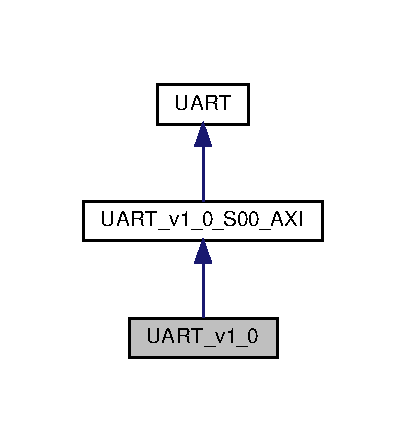
\includegraphics[width=195pt]{classUART__v1__0__inherit__graph}
\end{center}
\end{figure}


Collaboration diagram for U\+A\+R\+T\+\_\+v1\+\_\+0\+:
\nopagebreak
\begin{figure}[H]
\begin{center}
\leavevmode
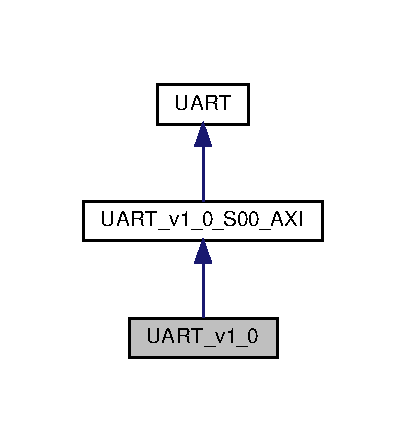
\includegraphics[width=195pt]{classUART__v1__0__coll__graph}
\end{center}
\end{figure}
\subsection*{Entities}
\begin{DoxyCompactItemize}
\item 
\hyperlink{classUART__v1__0_1_1arch__imp}{arch\+\_\+imp} architecture
\begin{DoxyCompactList}\small\item\em componente U\+A\+R\+T\+\_\+\+A\+X\+I\+\_\+\+S00  componente nel quale è incapsulato il componente \hyperlink{structUART}{U\+A\+RT} e la logica di gestione delle interruzioni. \end{DoxyCompactList}\end{DoxyCompactItemize}
\subsection*{Libraries}
 \begin{DoxyCompactItemize}
\item 
\mbox{\Hypertarget{classUART__v1__0_a0a6af6eef40212dbaf130d57ce711256}\label{classUART__v1__0_a0a6af6eef40212dbaf130d57ce711256}} 
\hyperlink{classUART__v1__0_a0a6af6eef40212dbaf130d57ce711256}{ieee} 
\begin{DoxyCompactList}\small\item\em Viene utilizzata la libreria I\+E\+EE. \end{DoxyCompactList}\end{DoxyCompactItemize}
\subsection*{Use Clauses}
 \begin{DoxyCompactItemize}
\item 
\mbox{\Hypertarget{classUART__v1__0_acd03516902501cd1c7296a98e22c6fcb}\label{classUART__v1__0_acd03516902501cd1c7296a98e22c6fcb}} 
\hyperlink{classUART__v1__0_acd03516902501cd1c7296a98e22c6fcb}{std\+\_\+logic\+\_\+1164}   
\begin{DoxyCompactList}\small\item\em Sono utilizzati i segnali della standard logic. \end{DoxyCompactList}\item 
\mbox{\Hypertarget{classUART__v1__0_a2edc34402b573437d5f25fa90ba4013e}\label{classUART__v1__0_a2edc34402b573437d5f25fa90ba4013e}} 
\hyperlink{classUART__v1__0_a2edc34402b573437d5f25fa90ba4013e}{numeric\+\_\+std}   
\begin{DoxyCompactList}\small\item\em Vengono utilizzate le funzioni numeriche. \end{DoxyCompactList}\end{DoxyCompactItemize}
\subsection*{Generics}
 \begin{DoxyCompactItemize}
\item 
\mbox{\Hypertarget{classUART__v1__0_af2979064a441fc814952a2a01b2e0bd3}\label{classUART__v1__0_af2979064a441fc814952a2a01b2e0bd3}} 
\hyperlink{classUART__v1__0_af2979064a441fc814952a2a01b2e0bd3}{baudrate} {\bfseries {\bfseries \textcolor{vhdlchar}{integer}\textcolor{vhdlchar}{ }\textcolor{vhdlchar}{ }\textcolor{vhdlchar}{\+:}\textcolor{vhdlchar}{=}\textcolor{vhdlchar}{ }\textcolor{vhdlchar}{ } \textcolor{vhdldigit}{9600} \textcolor{vhdlchar}{ }}}
\begin{DoxyCompactList}\small\item\em baudare trasmissione \end{DoxyCompactList}\item 
\mbox{\Hypertarget{classUART__v1__0_a378457a97325b4f40100f5b52b3dd886}\label{classUART__v1__0_a378457a97325b4f40100f5b52b3dd886}} 
\hyperlink{classUART__v1__0_a378457a97325b4f40100f5b52b3dd886}{clock\+\_\+freq} {\bfseries {\bfseries \textcolor{vhdlchar}{integer}\textcolor{vhdlchar}{ }\textcolor{vhdlchar}{ }\textcolor{vhdlchar}{\+:}\textcolor{vhdlchar}{=}\textcolor{vhdlchar}{ }\textcolor{vhdlchar}{ } \textcolor{vhdldigit}{50\+\_\+000\+\_\+000} \textcolor{vhdlchar}{ }}}
\begin{DoxyCompactList}\small\item\em frequenza clock ingresso \end{DoxyCompactList}\item 
\mbox{\Hypertarget{classUART__v1__0_afce7943994a4ddfa81f224225976a4c7}\label{classUART__v1__0_afce7943994a4ddfa81f224225976a4c7}} 
\hyperlink{classUART__v1__0_afce7943994a4ddfa81f224225976a4c7}{C\+\_\+\+S00\+\_\+\+A\+X\+I\+\_\+\+D\+A\+T\+A\+\_\+\+W\+I\+D\+TH} {\bfseries {\bfseries \textcolor{vhdlchar}{integer}\textcolor{vhdlchar}{ }\textcolor{vhdlchar}{ }\textcolor{vhdlchar}{\+:}\textcolor{vhdlchar}{=}\textcolor{vhdlchar}{ }\textcolor{vhdlchar}{ } \textcolor{vhdldigit}{32} \textcolor{vhdlchar}{ }}}
\item 
\mbox{\Hypertarget{classUART__v1__0_ab7787f274c76bb896ac98fdcfb570c65}\label{classUART__v1__0_ab7787f274c76bb896ac98fdcfb570c65}} 
\hyperlink{classUART__v1__0_ab7787f274c76bb896ac98fdcfb570c65}{C\+\_\+\+S00\+\_\+\+A\+X\+I\+\_\+\+A\+D\+D\+R\+\_\+\+W\+I\+D\+TH} {\bfseries {\bfseries \textcolor{vhdlchar}{integer}\textcolor{vhdlchar}{ }\textcolor{vhdlchar}{ }\textcolor{vhdlchar}{\+:}\textcolor{vhdlchar}{=}\textcolor{vhdlchar}{ }\textcolor{vhdlchar}{ } \textcolor{vhdldigit}{5} \textcolor{vhdlchar}{ }}}
\end{DoxyCompactItemize}
\subsection*{Ports}
 \begin{DoxyCompactItemize}
\item 
\mbox{\Hypertarget{classUART__v1__0_aa1eb566eeabe2a672e15ebb95aecc44f}\label{classUART__v1__0_aa1eb566eeabe2a672e15ebb95aecc44f}} 
\hyperlink{classUART__v1__0_aa1eb566eeabe2a672e15ebb95aecc44f}{tx}  {\bfseries {\bfseries \textcolor{vhdlchar}{out}\textcolor{vhdlchar}{ }}} {\bfseries \textcolor{vhdlchar}{std\+\_\+logic}\textcolor{vhdlchar}{ }} 
\begin{DoxyCompactList}\small\item\em linea uscita per la trasmissione \end{DoxyCompactList}\item 
\mbox{\Hypertarget{classUART__v1__0_a98ea5026beb91d6383a8a2aa2d69b32f}\label{classUART__v1__0_a98ea5026beb91d6383a8a2aa2d69b32f}} 
\hyperlink{classUART__v1__0_a98ea5026beb91d6383a8a2aa2d69b32f}{rx}  {\bfseries {\bfseries \textcolor{vhdlchar}{in}\textcolor{vhdlchar}{ }}} {\bfseries \textcolor{vhdlchar}{std\+\_\+logic}\textcolor{vhdlchar}{ }} 
\begin{DoxyCompactList}\small\item\em linea ingresso per la ricezione \end{DoxyCompactList}\item 
\mbox{\Hypertarget{classUART__v1__0_a5b78f3e3edfaf6e8ec79031b9e631e9d}\label{classUART__v1__0_a5b78f3e3edfaf6e8ec79031b9e631e9d}} 
\hyperlink{classUART__v1__0_a5b78f3e3edfaf6e8ec79031b9e631e9d}{interrupt}  {\bfseries {\bfseries \textcolor{vhdlchar}{out}\textcolor{vhdlchar}{ }}} {\bfseries \textcolor{vhdlchar}{std\+\_\+logic}\textcolor{vhdlchar}{ }} 
\begin{DoxyCompactList}\small\item\em segnale per richiede l\textquotesingle{}interrupt \end{DoxyCompactList}\item 
\mbox{\Hypertarget{classUART__v1__0_a037f9e3df8559bfd59db37bcba9cb7a8}\label{classUART__v1__0_a037f9e3df8559bfd59db37bcba9cb7a8}} 
\hyperlink{classUART__v1__0_a037f9e3df8559bfd59db37bcba9cb7a8}{s00\+\_\+axi\+\_\+aclk}  {\bfseries {\bfseries \textcolor{vhdlchar}{in}\textcolor{vhdlchar}{ }}} {\bfseries \textcolor{vhdlchar}{std\+\_\+logic}\textcolor{vhdlchar}{ }} 
\item 
\mbox{\Hypertarget{classUART__v1__0_a8249c106fbd80196dcad2666c9f0b3fc}\label{classUART__v1__0_a8249c106fbd80196dcad2666c9f0b3fc}} 
\hyperlink{classUART__v1__0_a8249c106fbd80196dcad2666c9f0b3fc}{s00\+\_\+axi\+\_\+aresetn}  {\bfseries {\bfseries \textcolor{vhdlchar}{in}\textcolor{vhdlchar}{ }}} {\bfseries \textcolor{vhdlchar}{std\+\_\+logic}\textcolor{vhdlchar}{ }} 
\item 
\mbox{\Hypertarget{classUART__v1__0_a9fe80d3cc7f862afb670536e4e05dbeb}\label{classUART__v1__0_a9fe80d3cc7f862afb670536e4e05dbeb}} 
\hyperlink{classUART__v1__0_a9fe80d3cc7f862afb670536e4e05dbeb}{s00\+\_\+axi\+\_\+awaddr}  {\bfseries {\bfseries \textcolor{vhdlchar}{in}\textcolor{vhdlchar}{ }}} {\bfseries \textcolor{vhdlchar}{std\+\_\+logic\+\_\+vector}\textcolor{vhdlchar}{ }\textcolor{vhdlchar}{(}\textcolor{vhdlchar}{ }\textcolor{vhdlchar}{ }\textcolor{vhdlchar}{ }\textcolor{vhdlchar}{ }\textcolor{vhdlchar}{C\+\_\+\+S00\+\_\+\+A\+X\+I\+\_\+\+A\+D\+D\+R\+\_\+\+W\+I\+D\+TH}\textcolor{vhdlchar}{-\/}\textcolor{vhdlchar}{ } \textcolor{vhdldigit}{1} \textcolor{vhdlchar}{ }\textcolor{vhdlchar}{downto}\textcolor{vhdlchar}{ }\textcolor{vhdlchar}{ } \textcolor{vhdldigit}{0} \textcolor{vhdlchar}{ }\textcolor{vhdlchar}{)}\textcolor{vhdlchar}{ }} 
\item 
\mbox{\Hypertarget{classUART__v1__0_a719659c1addef5432978cc949d9e10ed}\label{classUART__v1__0_a719659c1addef5432978cc949d9e10ed}} 
\hyperlink{classUART__v1__0_a719659c1addef5432978cc949d9e10ed}{s00\+\_\+axi\+\_\+awprot}  {\bfseries {\bfseries \textcolor{vhdlchar}{in}\textcolor{vhdlchar}{ }}} {\bfseries \textcolor{vhdlchar}{std\+\_\+logic\+\_\+vector}\textcolor{vhdlchar}{ }\textcolor{vhdlchar}{(}\textcolor{vhdlchar}{ }\textcolor{vhdlchar}{ } \textcolor{vhdldigit}{2} \textcolor{vhdlchar}{ }\textcolor{vhdlchar}{downto}\textcolor{vhdlchar}{ }\textcolor{vhdlchar}{ } \textcolor{vhdldigit}{0} \textcolor{vhdlchar}{ }\textcolor{vhdlchar}{)}\textcolor{vhdlchar}{ }} 
\item 
\mbox{\Hypertarget{classUART__v1__0_a45aa02a72ae1a8389346d47173c60ed0}\label{classUART__v1__0_a45aa02a72ae1a8389346d47173c60ed0}} 
\hyperlink{classUART__v1__0_a45aa02a72ae1a8389346d47173c60ed0}{s00\+\_\+axi\+\_\+awvalid}  {\bfseries {\bfseries \textcolor{vhdlchar}{in}\textcolor{vhdlchar}{ }}} {\bfseries \textcolor{vhdlchar}{std\+\_\+logic}\textcolor{vhdlchar}{ }} 
\item 
\mbox{\Hypertarget{classUART__v1__0_ad0a1f71502d91a45dbc6c365f85c6566}\label{classUART__v1__0_ad0a1f71502d91a45dbc6c365f85c6566}} 
\hyperlink{classUART__v1__0_ad0a1f71502d91a45dbc6c365f85c6566}{s00\+\_\+axi\+\_\+awready}  {\bfseries {\bfseries \textcolor{vhdlchar}{out}\textcolor{vhdlchar}{ }}} {\bfseries \textcolor{vhdlchar}{std\+\_\+logic}\textcolor{vhdlchar}{ }} 
\item 
\mbox{\Hypertarget{classUART__v1__0_ae2b15b55ee463fd9dd030ee29db6bb17}\label{classUART__v1__0_ae2b15b55ee463fd9dd030ee29db6bb17}} 
\hyperlink{classUART__v1__0_ae2b15b55ee463fd9dd030ee29db6bb17}{s00\+\_\+axi\+\_\+wdata}  {\bfseries {\bfseries \textcolor{vhdlchar}{in}\textcolor{vhdlchar}{ }}} {\bfseries \textcolor{vhdlchar}{std\+\_\+logic\+\_\+vector}\textcolor{vhdlchar}{ }\textcolor{vhdlchar}{(}\textcolor{vhdlchar}{ }\textcolor{vhdlchar}{ }\textcolor{vhdlchar}{ }\textcolor{vhdlchar}{ }\textcolor{vhdlchar}{C\+\_\+\+S00\+\_\+\+A\+X\+I\+\_\+\+D\+A\+T\+A\+\_\+\+W\+I\+D\+TH}\textcolor{vhdlchar}{-\/}\textcolor{vhdlchar}{ } \textcolor{vhdldigit}{1} \textcolor{vhdlchar}{ }\textcolor{vhdlchar}{downto}\textcolor{vhdlchar}{ }\textcolor{vhdlchar}{ } \textcolor{vhdldigit}{0} \textcolor{vhdlchar}{ }\textcolor{vhdlchar}{)}\textcolor{vhdlchar}{ }} 
\item 
\mbox{\Hypertarget{classUART__v1__0_a120924bc3fd5fd10ec0f96e19c3f4904}\label{classUART__v1__0_a120924bc3fd5fd10ec0f96e19c3f4904}} 
\hyperlink{classUART__v1__0_a120924bc3fd5fd10ec0f96e19c3f4904}{s00\+\_\+axi\+\_\+wstrb}  {\bfseries {\bfseries \textcolor{vhdlchar}{in}\textcolor{vhdlchar}{ }}} {\bfseries \textcolor{vhdlchar}{std\+\_\+logic\+\_\+vector}\textcolor{vhdlchar}{ }\textcolor{vhdlchar}{(}\textcolor{vhdlchar}{ }\textcolor{vhdlchar}{(}\textcolor{vhdlchar}{ }\textcolor{vhdlchar}{ }\textcolor{vhdlchar}{ }\textcolor{vhdlchar}{ }\textcolor{vhdlchar}{C\+\_\+\+S00\+\_\+\+A\+X\+I\+\_\+\+D\+A\+T\+A\+\_\+\+W\+I\+D\+TH}\textcolor{vhdlchar}{/}\textcolor{vhdlchar}{ } \textcolor{vhdldigit}{8} \textcolor{vhdlchar}{ }\textcolor{vhdlchar}{)}\textcolor{vhdlchar}{ }\textcolor{vhdlchar}{-\/}\textcolor{vhdlchar}{ } \textcolor{vhdldigit}{1} \textcolor{vhdlchar}{ }\textcolor{vhdlchar}{downto}\textcolor{vhdlchar}{ }\textcolor{vhdlchar}{ } \textcolor{vhdldigit}{0} \textcolor{vhdlchar}{ }\textcolor{vhdlchar}{)}\textcolor{vhdlchar}{ }} 
\item 
\mbox{\Hypertarget{classUART__v1__0_a24e90907193647007d2947353740114d}\label{classUART__v1__0_a24e90907193647007d2947353740114d}} 
\hyperlink{classUART__v1__0_a24e90907193647007d2947353740114d}{s00\+\_\+axi\+\_\+wvalid}  {\bfseries {\bfseries \textcolor{vhdlchar}{in}\textcolor{vhdlchar}{ }}} {\bfseries \textcolor{vhdlchar}{std\+\_\+logic}\textcolor{vhdlchar}{ }} 
\item 
\mbox{\Hypertarget{classUART__v1__0_a3fc60abc0cfbfa90003a83bffdd476c4}\label{classUART__v1__0_a3fc60abc0cfbfa90003a83bffdd476c4}} 
\hyperlink{classUART__v1__0_a3fc60abc0cfbfa90003a83bffdd476c4}{s00\+\_\+axi\+\_\+wready}  {\bfseries {\bfseries \textcolor{vhdlchar}{out}\textcolor{vhdlchar}{ }}} {\bfseries \textcolor{vhdlchar}{std\+\_\+logic}\textcolor{vhdlchar}{ }} 
\item 
\mbox{\Hypertarget{classUART__v1__0_af8799be946d3f5354263e7deb15f94f1}\label{classUART__v1__0_af8799be946d3f5354263e7deb15f94f1}} 
\hyperlink{classUART__v1__0_af8799be946d3f5354263e7deb15f94f1}{s00\+\_\+axi\+\_\+bresp}  {\bfseries {\bfseries \textcolor{vhdlchar}{out}\textcolor{vhdlchar}{ }}} {\bfseries \textcolor{vhdlchar}{std\+\_\+logic\+\_\+vector}\textcolor{vhdlchar}{ }\textcolor{vhdlchar}{(}\textcolor{vhdlchar}{ }\textcolor{vhdlchar}{ } \textcolor{vhdldigit}{1} \textcolor{vhdlchar}{ }\textcolor{vhdlchar}{downto}\textcolor{vhdlchar}{ }\textcolor{vhdlchar}{ } \textcolor{vhdldigit}{0} \textcolor{vhdlchar}{ }\textcolor{vhdlchar}{)}\textcolor{vhdlchar}{ }} 
\item 
\mbox{\Hypertarget{classUART__v1__0_a5110b7dd4fb9548a2aab88f50dbe1d5e}\label{classUART__v1__0_a5110b7dd4fb9548a2aab88f50dbe1d5e}} 
\hyperlink{classUART__v1__0_a5110b7dd4fb9548a2aab88f50dbe1d5e}{s00\+\_\+axi\+\_\+bvalid}  {\bfseries {\bfseries \textcolor{vhdlchar}{out}\textcolor{vhdlchar}{ }}} {\bfseries \textcolor{vhdlchar}{std\+\_\+logic}\textcolor{vhdlchar}{ }} 
\item 
\mbox{\Hypertarget{classUART__v1__0_a1ef2019b0613bc23d4829eeeb24eb98d}\label{classUART__v1__0_a1ef2019b0613bc23d4829eeeb24eb98d}} 
\hyperlink{classUART__v1__0_a1ef2019b0613bc23d4829eeeb24eb98d}{s00\+\_\+axi\+\_\+bready}  {\bfseries {\bfseries \textcolor{vhdlchar}{in}\textcolor{vhdlchar}{ }}} {\bfseries \textcolor{vhdlchar}{std\+\_\+logic}\textcolor{vhdlchar}{ }} 
\item 
\mbox{\Hypertarget{classUART__v1__0_af70a86336cd6505064e45b69f4623939}\label{classUART__v1__0_af70a86336cd6505064e45b69f4623939}} 
\hyperlink{classUART__v1__0_af70a86336cd6505064e45b69f4623939}{s00\+\_\+axi\+\_\+araddr}  {\bfseries {\bfseries \textcolor{vhdlchar}{in}\textcolor{vhdlchar}{ }}} {\bfseries \textcolor{vhdlchar}{std\+\_\+logic\+\_\+vector}\textcolor{vhdlchar}{ }\textcolor{vhdlchar}{(}\textcolor{vhdlchar}{ }\textcolor{vhdlchar}{ }\textcolor{vhdlchar}{ }\textcolor{vhdlchar}{ }\textcolor{vhdlchar}{C\+\_\+\+S00\+\_\+\+A\+X\+I\+\_\+\+A\+D\+D\+R\+\_\+\+W\+I\+D\+TH}\textcolor{vhdlchar}{-\/}\textcolor{vhdlchar}{ } \textcolor{vhdldigit}{1} \textcolor{vhdlchar}{ }\textcolor{vhdlchar}{downto}\textcolor{vhdlchar}{ }\textcolor{vhdlchar}{ } \textcolor{vhdldigit}{0} \textcolor{vhdlchar}{ }\textcolor{vhdlchar}{)}\textcolor{vhdlchar}{ }} 
\item 
\mbox{\Hypertarget{classUART__v1__0_adc648df07895bf808b8c721e1dc6811b}\label{classUART__v1__0_adc648df07895bf808b8c721e1dc6811b}} 
\hyperlink{classUART__v1__0_adc648df07895bf808b8c721e1dc6811b}{s00\+\_\+axi\+\_\+arprot}  {\bfseries {\bfseries \textcolor{vhdlchar}{in}\textcolor{vhdlchar}{ }}} {\bfseries \textcolor{vhdlchar}{std\+\_\+logic\+\_\+vector}\textcolor{vhdlchar}{ }\textcolor{vhdlchar}{(}\textcolor{vhdlchar}{ }\textcolor{vhdlchar}{ } \textcolor{vhdldigit}{2} \textcolor{vhdlchar}{ }\textcolor{vhdlchar}{downto}\textcolor{vhdlchar}{ }\textcolor{vhdlchar}{ } \textcolor{vhdldigit}{0} \textcolor{vhdlchar}{ }\textcolor{vhdlchar}{)}\textcolor{vhdlchar}{ }} 
\item 
\mbox{\Hypertarget{classUART__v1__0_a94b78b2ae3cd13860f15afbdfb199e44}\label{classUART__v1__0_a94b78b2ae3cd13860f15afbdfb199e44}} 
\hyperlink{classUART__v1__0_a94b78b2ae3cd13860f15afbdfb199e44}{s00\+\_\+axi\+\_\+arvalid}  {\bfseries {\bfseries \textcolor{vhdlchar}{in}\textcolor{vhdlchar}{ }}} {\bfseries \textcolor{vhdlchar}{std\+\_\+logic}\textcolor{vhdlchar}{ }} 
\item 
\mbox{\Hypertarget{classUART__v1__0_ad35bd95f3352ff8dbdaea55205a98e53}\label{classUART__v1__0_ad35bd95f3352ff8dbdaea55205a98e53}} 
\hyperlink{classUART__v1__0_ad35bd95f3352ff8dbdaea55205a98e53}{s00\+\_\+axi\+\_\+arready}  {\bfseries {\bfseries \textcolor{vhdlchar}{out}\textcolor{vhdlchar}{ }}} {\bfseries \textcolor{vhdlchar}{std\+\_\+logic}\textcolor{vhdlchar}{ }} 
\item 
\mbox{\Hypertarget{classUART__v1__0_ad2655fadb987e0487c428aca187b55d0}\label{classUART__v1__0_ad2655fadb987e0487c428aca187b55d0}} 
\hyperlink{classUART__v1__0_ad2655fadb987e0487c428aca187b55d0}{s00\+\_\+axi\+\_\+rdata}  {\bfseries {\bfseries \textcolor{vhdlchar}{out}\textcolor{vhdlchar}{ }}} {\bfseries \textcolor{vhdlchar}{std\+\_\+logic\+\_\+vector}\textcolor{vhdlchar}{ }\textcolor{vhdlchar}{(}\textcolor{vhdlchar}{ }\textcolor{vhdlchar}{ }\textcolor{vhdlchar}{ }\textcolor{vhdlchar}{ }\textcolor{vhdlchar}{C\+\_\+\+S00\+\_\+\+A\+X\+I\+\_\+\+D\+A\+T\+A\+\_\+\+W\+I\+D\+TH}\textcolor{vhdlchar}{-\/}\textcolor{vhdlchar}{ } \textcolor{vhdldigit}{1} \textcolor{vhdlchar}{ }\textcolor{vhdlchar}{downto}\textcolor{vhdlchar}{ }\textcolor{vhdlchar}{ } \textcolor{vhdldigit}{0} \textcolor{vhdlchar}{ }\textcolor{vhdlchar}{)}\textcolor{vhdlchar}{ }} 
\item 
\mbox{\Hypertarget{classUART__v1__0_a1acee955f50f71e5595a03c6ca301cf0}\label{classUART__v1__0_a1acee955f50f71e5595a03c6ca301cf0}} 
\hyperlink{classUART__v1__0_a1acee955f50f71e5595a03c6ca301cf0}{s00\+\_\+axi\+\_\+rresp}  {\bfseries {\bfseries \textcolor{vhdlchar}{out}\textcolor{vhdlchar}{ }}} {\bfseries \textcolor{vhdlchar}{std\+\_\+logic\+\_\+vector}\textcolor{vhdlchar}{ }\textcolor{vhdlchar}{(}\textcolor{vhdlchar}{ }\textcolor{vhdlchar}{ } \textcolor{vhdldigit}{1} \textcolor{vhdlchar}{ }\textcolor{vhdlchar}{downto}\textcolor{vhdlchar}{ }\textcolor{vhdlchar}{ } \textcolor{vhdldigit}{0} \textcolor{vhdlchar}{ }\textcolor{vhdlchar}{)}\textcolor{vhdlchar}{ }} 
\item 
\mbox{\Hypertarget{classUART__v1__0_af180911f7eb262e530e26865bc97aa0b}\label{classUART__v1__0_af180911f7eb262e530e26865bc97aa0b}} 
\hyperlink{classUART__v1__0_af180911f7eb262e530e26865bc97aa0b}{s00\+\_\+axi\+\_\+rvalid}  {\bfseries {\bfseries \textcolor{vhdlchar}{out}\textcolor{vhdlchar}{ }}} {\bfseries \textcolor{vhdlchar}{std\+\_\+logic}\textcolor{vhdlchar}{ }} 
\item 
\mbox{\Hypertarget{classUART__v1__0_a8b82eb165d7024f6c7b25646f6ebdd4d}\label{classUART__v1__0_a8b82eb165d7024f6c7b25646f6ebdd4d}} 
\hyperlink{classUART__v1__0_a8b82eb165d7024f6c7b25646f6ebdd4d}{s00\+\_\+axi\+\_\+rready}  {\bfseries {\bfseries \textcolor{vhdlchar}{in}\textcolor{vhdlchar}{ }}} {\bfseries \textcolor{vhdlchar}{std\+\_\+logic}\textcolor{vhdlchar}{ }} 
\end{DoxyCompactItemize}


The documentation for this class was generated from the following file\+:\begin{DoxyCompactItemize}
\item 
/media/saverio/\+O\+S/\+Users/\+Saverio/\+Desktop/\+S\+E/git/\+Andrea/\+F\+P\+G\+A/ip\+\_\+repo/\+U\+A\+R\+T\+\_\+1.\+0/hdl/\hyperlink{UART__v1__0_8vhd}{U\+A\+R\+T\+\_\+v1\+\_\+0.\+vhd}\end{DoxyCompactItemize}

\hypertarget{classUART__v1__0__S00__AXI}{}\section{U\+A\+R\+T\+\_\+v1\+\_\+0\+\_\+\+S00\+\_\+\+A\+XI Entity Reference}
\label{classUART__v1__0__S00__AXI}\index{U\+A\+R\+T\+\_\+v1\+\_\+0\+\_\+\+S00\+\_\+\+A\+XI@{U\+A\+R\+T\+\_\+v1\+\_\+0\+\_\+\+S00\+\_\+\+A\+XI}}


Inheritance diagram for U\+A\+R\+T\+\_\+v1\+\_\+0\+\_\+\+S00\+\_\+\+A\+XI\+:\nopagebreak
\begin{figure}[H]
\begin{center}
\leavevmode
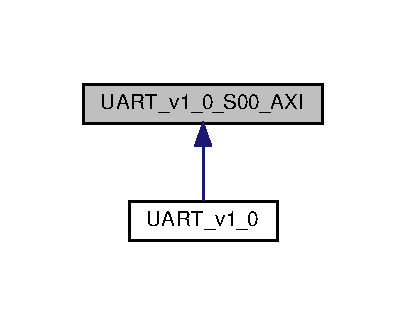
\includegraphics[width=195pt]{classUART__v1__0__S00__AXI__inherit__graph}
\end{center}
\end{figure}


Collaboration diagram for U\+A\+R\+T\+\_\+v1\+\_\+0\+\_\+\+S00\+\_\+\+A\+XI\+:\nopagebreak
\begin{figure}[H]
\begin{center}
\leavevmode
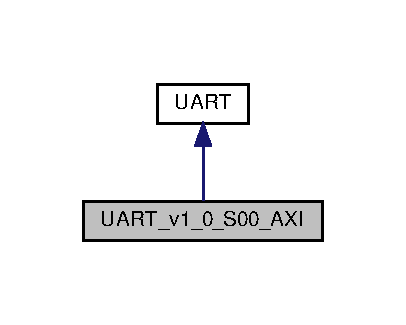
\includegraphics[width=195pt]{classUART__v1__0__S00__AXI__coll__graph}
\end{center}
\end{figure}
\subsection*{Entities}
\begin{DoxyCompactItemize}
\item 
\hyperlink{classUART__v1__0__S00__AXI_1_1arch__imp}{arch\+\_\+imp} architecture
\end{DoxyCompactItemize}
\subsection*{Libraries}
 \begin{DoxyCompactItemize}
\item 
\mbox{\Hypertarget{classUART__v1__0__S00__AXI_a0a6af6eef40212dbaf130d57ce711256}\label{classUART__v1__0__S00__AXI_a0a6af6eef40212dbaf130d57ce711256}} 
\hyperlink{classUART__v1__0__S00__AXI_a0a6af6eef40212dbaf130d57ce711256}{ieee} 
\begin{DoxyCompactList}\small\item\em Viene utilizzata la libreria I\+E\+EE. \end{DoxyCompactList}\end{DoxyCompactItemize}
\subsection*{Use Clauses}
 \begin{DoxyCompactItemize}
\item 
\mbox{\Hypertarget{classUART__v1__0__S00__AXI_acd03516902501cd1c7296a98e22c6fcb}\label{classUART__v1__0__S00__AXI_acd03516902501cd1c7296a98e22c6fcb}} 
\hyperlink{classUART__v1__0__S00__AXI_acd03516902501cd1c7296a98e22c6fcb}{std\+\_\+logic\+\_\+1164}   
\begin{DoxyCompactList}\small\item\em Sono utilizzati i segnali della standard logic. \end{DoxyCompactList}\item 
\mbox{\Hypertarget{classUART__v1__0__S00__AXI_a2edc34402b573437d5f25fa90ba4013e}\label{classUART__v1__0__S00__AXI_a2edc34402b573437d5f25fa90ba4013e}} 
\hyperlink{classUART__v1__0__S00__AXI_a2edc34402b573437d5f25fa90ba4013e}{numeric\+\_\+std}   
\begin{DoxyCompactList}\small\item\em Vengono utilizzate le funzioni numeriche. \end{DoxyCompactList}\item 
\mbox{\Hypertarget{classUART__v1__0__S00__AXI_acb2d98d781f19c8f5f4109576ec45502}\label{classUART__v1__0__S00__AXI_acb2d98d781f19c8f5f4109576ec45502}} 
\hyperlink{classUART__v1__0__S00__AXI_acb2d98d781f19c8f5f4109576ec45502}{std\+\_\+logic\+\_\+misc}   
\begin{DoxyCompactList}\small\item\em libreria necessaria per la funzione or\+\_\+reduce \end{DoxyCompactList}\end{DoxyCompactItemize}
\subsection*{Generics}
 \begin{DoxyCompactItemize}
\item 
\mbox{\Hypertarget{classUART__v1__0__S00__AXI_af2979064a441fc814952a2a01b2e0bd3}\label{classUART__v1__0__S00__AXI_af2979064a441fc814952a2a01b2e0bd3}} 
\hyperlink{classUART__v1__0__S00__AXI_af2979064a441fc814952a2a01b2e0bd3}{baudrate} {\bfseries {\bfseries \textcolor{vhdlchar}{integer}\textcolor{vhdlchar}{ }\textcolor{vhdlchar}{ }\textcolor{vhdlchar}{\+:}\textcolor{vhdlchar}{=}\textcolor{vhdlchar}{ }\textcolor{vhdlchar}{ } \textcolor{vhdldigit}{9600} \textcolor{vhdlchar}{ }}}
\item 
\mbox{\Hypertarget{classUART__v1__0__S00__AXI_a378457a97325b4f40100f5b52b3dd886}\label{classUART__v1__0__S00__AXI_a378457a97325b4f40100f5b52b3dd886}} 
\hyperlink{classUART__v1__0__S00__AXI_a378457a97325b4f40100f5b52b3dd886}{clock\+\_\+freq} {\bfseries {\bfseries \textcolor{vhdlchar}{integer}\textcolor{vhdlchar}{ }\textcolor{vhdlchar}{ }\textcolor{vhdlchar}{\+:}\textcolor{vhdlchar}{=}\textcolor{vhdlchar}{ }\textcolor{vhdlchar}{ } \textcolor{vhdldigit}{50\+\_\+000\+\_\+000} \textcolor{vhdlchar}{ }}}
\item 
\mbox{\Hypertarget{classUART__v1__0__S00__AXI_a0fad312acd1f302ce7de30c5658df0bd}\label{classUART__v1__0__S00__AXI_a0fad312acd1f302ce7de30c5658df0bd}} 
\hyperlink{classUART__v1__0__S00__AXI_a0fad312acd1f302ce7de30c5658df0bd}{C\+\_\+\+S\+\_\+\+A\+X\+I\+\_\+\+D\+A\+T\+A\+\_\+\+W\+I\+D\+TH} {\bfseries {\bfseries \textcolor{vhdlchar}{integer}\textcolor{vhdlchar}{ }\textcolor{vhdlchar}{ }\textcolor{vhdlchar}{\+:}\textcolor{vhdlchar}{=}\textcolor{vhdlchar}{ }\textcolor{vhdlchar}{ } \textcolor{vhdldigit}{32} \textcolor{vhdlchar}{ }}}
\item 
\mbox{\Hypertarget{classUART__v1__0__S00__AXI_a9abff2eaa069440f3b7d9e9937d5ee8e}\label{classUART__v1__0__S00__AXI_a9abff2eaa069440f3b7d9e9937d5ee8e}} 
\hyperlink{classUART__v1__0__S00__AXI_a9abff2eaa069440f3b7d9e9937d5ee8e}{C\+\_\+\+S\+\_\+\+A\+X\+I\+\_\+\+A\+D\+D\+R\+\_\+\+W\+I\+D\+TH} {\bfseries {\bfseries \textcolor{vhdlchar}{integer}\textcolor{vhdlchar}{ }\textcolor{vhdlchar}{ }\textcolor{vhdlchar}{\+:}\textcolor{vhdlchar}{=}\textcolor{vhdlchar}{ }\textcolor{vhdlchar}{ } \textcolor{vhdldigit}{5} \textcolor{vhdlchar}{ }}}
\end{DoxyCompactItemize}
\subsection*{Ports}
 \begin{DoxyCompactItemize}
\item 
\mbox{\Hypertarget{classUART__v1__0__S00__AXI_aa1eb566eeabe2a672e15ebb95aecc44f}\label{classUART__v1__0__S00__AXI_aa1eb566eeabe2a672e15ebb95aecc44f}} 
\hyperlink{classUART__v1__0__S00__AXI_aa1eb566eeabe2a672e15ebb95aecc44f}{tx}  {\bfseries {\bfseries \textcolor{vhdlchar}{out}\textcolor{vhdlchar}{ }}} {\bfseries \textcolor{vhdlchar}{std\+\_\+logic}\textcolor{vhdlchar}{ }} 
\item 
\mbox{\Hypertarget{classUART__v1__0__S00__AXI_a98ea5026beb91d6383a8a2aa2d69b32f}\label{classUART__v1__0__S00__AXI_a98ea5026beb91d6383a8a2aa2d69b32f}} 
\hyperlink{classUART__v1__0__S00__AXI_a98ea5026beb91d6383a8a2aa2d69b32f}{rx}  {\bfseries {\bfseries \textcolor{vhdlchar}{in}\textcolor{vhdlchar}{ }}} {\bfseries \textcolor{vhdlchar}{std\+\_\+logic}\textcolor{vhdlchar}{ }} 
\item 
\mbox{\Hypertarget{classUART__v1__0__S00__AXI_a5b78f3e3edfaf6e8ec79031b9e631e9d}\label{classUART__v1__0__S00__AXI_a5b78f3e3edfaf6e8ec79031b9e631e9d}} 
\hyperlink{classUART__v1__0__S00__AXI_a5b78f3e3edfaf6e8ec79031b9e631e9d}{interrupt}  {\bfseries {\bfseries \textcolor{vhdlchar}{out}\textcolor{vhdlchar}{ }}} {\bfseries \textcolor{vhdlchar}{std\+\_\+logic}\textcolor{vhdlchar}{ }} 
\item 
\mbox{\Hypertarget{classUART__v1__0__S00__AXI_a3f54d782a88290bdaa6baffd7cd84ab4}\label{classUART__v1__0__S00__AXI_a3f54d782a88290bdaa6baffd7cd84ab4}} 
\hyperlink{classUART__v1__0__S00__AXI_a3f54d782a88290bdaa6baffd7cd84ab4}{S\+\_\+\+A\+X\+I\+\_\+\+A\+C\+LK}  {\bfseries {\bfseries \textcolor{vhdlchar}{in}\textcolor{vhdlchar}{ }}} {\bfseries \textcolor{vhdlchar}{std\+\_\+logic}\textcolor{vhdlchar}{ }} 
\item 
\mbox{\Hypertarget{classUART__v1__0__S00__AXI_a089b396e17dee353ccc7d5389dda5532}\label{classUART__v1__0__S00__AXI_a089b396e17dee353ccc7d5389dda5532}} 
\hyperlink{classUART__v1__0__S00__AXI_a089b396e17dee353ccc7d5389dda5532}{S\+\_\+\+A\+X\+I\+\_\+\+A\+R\+E\+S\+E\+TN}  {\bfseries {\bfseries \textcolor{vhdlchar}{in}\textcolor{vhdlchar}{ }}} {\bfseries \textcolor{vhdlchar}{std\+\_\+logic}\textcolor{vhdlchar}{ }} 
\item 
\mbox{\Hypertarget{classUART__v1__0__S00__AXI_a61cc7b190ba9d540e56941330e4a0883}\label{classUART__v1__0__S00__AXI_a61cc7b190ba9d540e56941330e4a0883}} 
\hyperlink{classUART__v1__0__S00__AXI_a61cc7b190ba9d540e56941330e4a0883}{S\+\_\+\+A\+X\+I\+\_\+\+A\+W\+A\+D\+DR}  {\bfseries {\bfseries \textcolor{vhdlchar}{in}\textcolor{vhdlchar}{ }}} {\bfseries \textcolor{vhdlchar}{std\+\_\+logic\+\_\+vector}\textcolor{vhdlchar}{ }\textcolor{vhdlchar}{(}\textcolor{vhdlchar}{ }\textcolor{vhdlchar}{ }\textcolor{vhdlchar}{ }\textcolor{vhdlchar}{ }\textcolor{vhdlchar}{C\+\_\+\+S\+\_\+\+A\+X\+I\+\_\+\+A\+D\+D\+R\+\_\+\+W\+I\+D\+TH}\textcolor{vhdlchar}{-\/}\textcolor{vhdlchar}{ } \textcolor{vhdldigit}{1} \textcolor{vhdlchar}{ }\textcolor{vhdlchar}{downto}\textcolor{vhdlchar}{ }\textcolor{vhdlchar}{ } \textcolor{vhdldigit}{0} \textcolor{vhdlchar}{ }\textcolor{vhdlchar}{)}\textcolor{vhdlchar}{ }} 
\item 
\mbox{\Hypertarget{classUART__v1__0__S00__AXI_a459abcd98567ad24261377eed899593a}\label{classUART__v1__0__S00__AXI_a459abcd98567ad24261377eed899593a}} 
\hyperlink{classUART__v1__0__S00__AXI_a459abcd98567ad24261377eed899593a}{S\+\_\+\+A\+X\+I\+\_\+\+A\+W\+P\+R\+OT}  {\bfseries {\bfseries \textcolor{vhdlchar}{in}\textcolor{vhdlchar}{ }}} {\bfseries \textcolor{vhdlchar}{std\+\_\+logic\+\_\+vector}\textcolor{vhdlchar}{ }\textcolor{vhdlchar}{(}\textcolor{vhdlchar}{ }\textcolor{vhdlchar}{ } \textcolor{vhdldigit}{2} \textcolor{vhdlchar}{ }\textcolor{vhdlchar}{downto}\textcolor{vhdlchar}{ }\textcolor{vhdlchar}{ } \textcolor{vhdldigit}{0} \textcolor{vhdlchar}{ }\textcolor{vhdlchar}{)}\textcolor{vhdlchar}{ }} 
\item 
\mbox{\Hypertarget{classUART__v1__0__S00__AXI_af1f1cbf67bf647ba58353c261719a3a0}\label{classUART__v1__0__S00__AXI_af1f1cbf67bf647ba58353c261719a3a0}} 
\hyperlink{classUART__v1__0__S00__AXI_af1f1cbf67bf647ba58353c261719a3a0}{S\+\_\+\+A\+X\+I\+\_\+\+A\+W\+V\+A\+L\+ID}  {\bfseries {\bfseries \textcolor{vhdlchar}{in}\textcolor{vhdlchar}{ }}} {\bfseries \textcolor{vhdlchar}{std\+\_\+logic}\textcolor{vhdlchar}{ }} 
\item 
\mbox{\Hypertarget{classUART__v1__0__S00__AXI_ac04aab5cc834e762e893e061016921c6}\label{classUART__v1__0__S00__AXI_ac04aab5cc834e762e893e061016921c6}} 
\hyperlink{classUART__v1__0__S00__AXI_ac04aab5cc834e762e893e061016921c6}{S\+\_\+\+A\+X\+I\+\_\+\+A\+W\+R\+E\+A\+DY}  {\bfseries {\bfseries \textcolor{vhdlchar}{out}\textcolor{vhdlchar}{ }}} {\bfseries \textcolor{vhdlchar}{std\+\_\+logic}\textcolor{vhdlchar}{ }} 
\item 
\mbox{\Hypertarget{classUART__v1__0__S00__AXI_a292e5db13719faf3a8b3aab091773467}\label{classUART__v1__0__S00__AXI_a292e5db13719faf3a8b3aab091773467}} 
\hyperlink{classUART__v1__0__S00__AXI_a292e5db13719faf3a8b3aab091773467}{S\+\_\+\+A\+X\+I\+\_\+\+W\+D\+A\+TA}  {\bfseries {\bfseries \textcolor{vhdlchar}{in}\textcolor{vhdlchar}{ }}} {\bfseries \textcolor{vhdlchar}{std\+\_\+logic\+\_\+vector}\textcolor{vhdlchar}{ }\textcolor{vhdlchar}{(}\textcolor{vhdlchar}{ }\textcolor{vhdlchar}{ }\textcolor{vhdlchar}{ }\textcolor{vhdlchar}{ }\textcolor{vhdlchar}{C\+\_\+\+S\+\_\+\+A\+X\+I\+\_\+\+D\+A\+T\+A\+\_\+\+W\+I\+D\+TH}\textcolor{vhdlchar}{-\/}\textcolor{vhdlchar}{ } \textcolor{vhdldigit}{1} \textcolor{vhdlchar}{ }\textcolor{vhdlchar}{downto}\textcolor{vhdlchar}{ }\textcolor{vhdlchar}{ } \textcolor{vhdldigit}{0} \textcolor{vhdlchar}{ }\textcolor{vhdlchar}{)}\textcolor{vhdlchar}{ }} 
\item 
\mbox{\Hypertarget{classUART__v1__0__S00__AXI_accd8e04b79540b57ab15fee1cb6c04f5}\label{classUART__v1__0__S00__AXI_accd8e04b79540b57ab15fee1cb6c04f5}} 
\hyperlink{classUART__v1__0__S00__AXI_accd8e04b79540b57ab15fee1cb6c04f5}{S\+\_\+\+A\+X\+I\+\_\+\+W\+S\+T\+RB}  {\bfseries {\bfseries \textcolor{vhdlchar}{in}\textcolor{vhdlchar}{ }}} {\bfseries \textcolor{vhdlchar}{std\+\_\+logic\+\_\+vector}\textcolor{vhdlchar}{ }\textcolor{vhdlchar}{(}\textcolor{vhdlchar}{ }\textcolor{vhdlchar}{(}\textcolor{vhdlchar}{ }\textcolor{vhdlchar}{ }\textcolor{vhdlchar}{ }\textcolor{vhdlchar}{ }\textcolor{vhdlchar}{C\+\_\+\+S\+\_\+\+A\+X\+I\+\_\+\+D\+A\+T\+A\+\_\+\+W\+I\+D\+TH}\textcolor{vhdlchar}{/}\textcolor{vhdlchar}{ } \textcolor{vhdldigit}{8} \textcolor{vhdlchar}{ }\textcolor{vhdlchar}{)}\textcolor{vhdlchar}{ }\textcolor{vhdlchar}{-\/}\textcolor{vhdlchar}{ } \textcolor{vhdldigit}{1} \textcolor{vhdlchar}{ }\textcolor{vhdlchar}{downto}\textcolor{vhdlchar}{ }\textcolor{vhdlchar}{ } \textcolor{vhdldigit}{0} \textcolor{vhdlchar}{ }\textcolor{vhdlchar}{)}\textcolor{vhdlchar}{ }} 
\item 
\mbox{\Hypertarget{classUART__v1__0__S00__AXI_a60bd882e2de781af9a7c6c3d494225d5}\label{classUART__v1__0__S00__AXI_a60bd882e2de781af9a7c6c3d494225d5}} 
\hyperlink{classUART__v1__0__S00__AXI_a60bd882e2de781af9a7c6c3d494225d5}{S\+\_\+\+A\+X\+I\+\_\+\+W\+V\+A\+L\+ID}  {\bfseries {\bfseries \textcolor{vhdlchar}{in}\textcolor{vhdlchar}{ }}} {\bfseries \textcolor{vhdlchar}{std\+\_\+logic}\textcolor{vhdlchar}{ }} 
\item 
\mbox{\Hypertarget{classUART__v1__0__S00__AXI_ab84e4db7037141a360c2b59f45124f01}\label{classUART__v1__0__S00__AXI_ab84e4db7037141a360c2b59f45124f01}} 
\hyperlink{classUART__v1__0__S00__AXI_ab84e4db7037141a360c2b59f45124f01}{S\+\_\+\+A\+X\+I\+\_\+\+W\+R\+E\+A\+DY}  {\bfseries {\bfseries \textcolor{vhdlchar}{out}\textcolor{vhdlchar}{ }}} {\bfseries \textcolor{vhdlchar}{std\+\_\+logic}\textcolor{vhdlchar}{ }} 
\item 
\mbox{\Hypertarget{classUART__v1__0__S00__AXI_abca6c9777b38a5a6bc04886924bafcc8}\label{classUART__v1__0__S00__AXI_abca6c9777b38a5a6bc04886924bafcc8}} 
\hyperlink{classUART__v1__0__S00__AXI_abca6c9777b38a5a6bc04886924bafcc8}{S\+\_\+\+A\+X\+I\+\_\+\+B\+R\+E\+SP}  {\bfseries {\bfseries \textcolor{vhdlchar}{out}\textcolor{vhdlchar}{ }}} {\bfseries \textcolor{vhdlchar}{std\+\_\+logic\+\_\+vector}\textcolor{vhdlchar}{ }\textcolor{vhdlchar}{(}\textcolor{vhdlchar}{ }\textcolor{vhdlchar}{ } \textcolor{vhdldigit}{1} \textcolor{vhdlchar}{ }\textcolor{vhdlchar}{downto}\textcolor{vhdlchar}{ }\textcolor{vhdlchar}{ } \textcolor{vhdldigit}{0} \textcolor{vhdlchar}{ }\textcolor{vhdlchar}{)}\textcolor{vhdlchar}{ }} 
\item 
\mbox{\Hypertarget{classUART__v1__0__S00__AXI_a58f260d3ebaa69be91bb65ff9211823b}\label{classUART__v1__0__S00__AXI_a58f260d3ebaa69be91bb65ff9211823b}} 
\hyperlink{classUART__v1__0__S00__AXI_a58f260d3ebaa69be91bb65ff9211823b}{S\+\_\+\+A\+X\+I\+\_\+\+B\+V\+A\+L\+ID}  {\bfseries {\bfseries \textcolor{vhdlchar}{out}\textcolor{vhdlchar}{ }}} {\bfseries \textcolor{vhdlchar}{std\+\_\+logic}\textcolor{vhdlchar}{ }} 
\item 
\mbox{\Hypertarget{classUART__v1__0__S00__AXI_ac265989978a2be832d278f63fc0f06cb}\label{classUART__v1__0__S00__AXI_ac265989978a2be832d278f63fc0f06cb}} 
\hyperlink{classUART__v1__0__S00__AXI_ac265989978a2be832d278f63fc0f06cb}{S\+\_\+\+A\+X\+I\+\_\+\+B\+R\+E\+A\+DY}  {\bfseries {\bfseries \textcolor{vhdlchar}{in}\textcolor{vhdlchar}{ }}} {\bfseries \textcolor{vhdlchar}{std\+\_\+logic}\textcolor{vhdlchar}{ }} 
\item 
\mbox{\Hypertarget{classUART__v1__0__S00__AXI_a4d1dc8ecac269479747e5ac52c70ac45}\label{classUART__v1__0__S00__AXI_a4d1dc8ecac269479747e5ac52c70ac45}} 
\hyperlink{classUART__v1__0__S00__AXI_a4d1dc8ecac269479747e5ac52c70ac45}{S\+\_\+\+A\+X\+I\+\_\+\+A\+R\+A\+D\+DR}  {\bfseries {\bfseries \textcolor{vhdlchar}{in}\textcolor{vhdlchar}{ }}} {\bfseries \textcolor{vhdlchar}{std\+\_\+logic\+\_\+vector}\textcolor{vhdlchar}{ }\textcolor{vhdlchar}{(}\textcolor{vhdlchar}{ }\textcolor{vhdlchar}{ }\textcolor{vhdlchar}{ }\textcolor{vhdlchar}{ }\textcolor{vhdlchar}{C\+\_\+\+S\+\_\+\+A\+X\+I\+\_\+\+A\+D\+D\+R\+\_\+\+W\+I\+D\+TH}\textcolor{vhdlchar}{-\/}\textcolor{vhdlchar}{ } \textcolor{vhdldigit}{1} \textcolor{vhdlchar}{ }\textcolor{vhdlchar}{downto}\textcolor{vhdlchar}{ }\textcolor{vhdlchar}{ } \textcolor{vhdldigit}{0} \textcolor{vhdlchar}{ }\textcolor{vhdlchar}{)}\textcolor{vhdlchar}{ }} 
\item 
\mbox{\Hypertarget{classUART__v1__0__S00__AXI_a30a07c47d3c1182bbb7c904483bb374f}\label{classUART__v1__0__S00__AXI_a30a07c47d3c1182bbb7c904483bb374f}} 
\hyperlink{classUART__v1__0__S00__AXI_a30a07c47d3c1182bbb7c904483bb374f}{S\+\_\+\+A\+X\+I\+\_\+\+A\+R\+P\+R\+OT}  {\bfseries {\bfseries \textcolor{vhdlchar}{in}\textcolor{vhdlchar}{ }}} {\bfseries \textcolor{vhdlchar}{std\+\_\+logic\+\_\+vector}\textcolor{vhdlchar}{ }\textcolor{vhdlchar}{(}\textcolor{vhdlchar}{ }\textcolor{vhdlchar}{ } \textcolor{vhdldigit}{2} \textcolor{vhdlchar}{ }\textcolor{vhdlchar}{downto}\textcolor{vhdlchar}{ }\textcolor{vhdlchar}{ } \textcolor{vhdldigit}{0} \textcolor{vhdlchar}{ }\textcolor{vhdlchar}{)}\textcolor{vhdlchar}{ }} 
\item 
\mbox{\Hypertarget{classUART__v1__0__S00__AXI_a758f6340dd3340ee46deafbae18a47b2}\label{classUART__v1__0__S00__AXI_a758f6340dd3340ee46deafbae18a47b2}} 
\hyperlink{classUART__v1__0__S00__AXI_a758f6340dd3340ee46deafbae18a47b2}{S\+\_\+\+A\+X\+I\+\_\+\+A\+R\+V\+A\+L\+ID}  {\bfseries {\bfseries \textcolor{vhdlchar}{in}\textcolor{vhdlchar}{ }}} {\bfseries \textcolor{vhdlchar}{std\+\_\+logic}\textcolor{vhdlchar}{ }} 
\item 
\mbox{\Hypertarget{classUART__v1__0__S00__AXI_ade4e78e9c32af26578fc5c74ca3197e8}\label{classUART__v1__0__S00__AXI_ade4e78e9c32af26578fc5c74ca3197e8}} 
\hyperlink{classUART__v1__0__S00__AXI_ade4e78e9c32af26578fc5c74ca3197e8}{S\+\_\+\+A\+X\+I\+\_\+\+A\+R\+R\+E\+A\+DY}  {\bfseries {\bfseries \textcolor{vhdlchar}{out}\textcolor{vhdlchar}{ }}} {\bfseries \textcolor{vhdlchar}{std\+\_\+logic}\textcolor{vhdlchar}{ }} 
\item 
\mbox{\Hypertarget{classUART__v1__0__S00__AXI_a194c6eff7c88405e7934dbc2425ee4ab}\label{classUART__v1__0__S00__AXI_a194c6eff7c88405e7934dbc2425ee4ab}} 
\hyperlink{classUART__v1__0__S00__AXI_a194c6eff7c88405e7934dbc2425ee4ab}{S\+\_\+\+A\+X\+I\+\_\+\+R\+D\+A\+TA}  {\bfseries {\bfseries \textcolor{vhdlchar}{out}\textcolor{vhdlchar}{ }}} {\bfseries \textcolor{vhdlchar}{std\+\_\+logic\+\_\+vector}\textcolor{vhdlchar}{ }\textcolor{vhdlchar}{(}\textcolor{vhdlchar}{ }\textcolor{vhdlchar}{ }\textcolor{vhdlchar}{ }\textcolor{vhdlchar}{ }\textcolor{vhdlchar}{C\+\_\+\+S\+\_\+\+A\+X\+I\+\_\+\+D\+A\+T\+A\+\_\+\+W\+I\+D\+TH}\textcolor{vhdlchar}{-\/}\textcolor{vhdlchar}{ } \textcolor{vhdldigit}{1} \textcolor{vhdlchar}{ }\textcolor{vhdlchar}{downto}\textcolor{vhdlchar}{ }\textcolor{vhdlchar}{ } \textcolor{vhdldigit}{0} \textcolor{vhdlchar}{ }\textcolor{vhdlchar}{)}\textcolor{vhdlchar}{ }} 
\item 
\mbox{\Hypertarget{classUART__v1__0__S00__AXI_a67ba85504b4c51fb0eb00d18fd70ad92}\label{classUART__v1__0__S00__AXI_a67ba85504b4c51fb0eb00d18fd70ad92}} 
\hyperlink{classUART__v1__0__S00__AXI_a67ba85504b4c51fb0eb00d18fd70ad92}{S\+\_\+\+A\+X\+I\+\_\+\+R\+R\+E\+SP}  {\bfseries {\bfseries \textcolor{vhdlchar}{out}\textcolor{vhdlchar}{ }}} {\bfseries \textcolor{vhdlchar}{std\+\_\+logic\+\_\+vector}\textcolor{vhdlchar}{ }\textcolor{vhdlchar}{(}\textcolor{vhdlchar}{ }\textcolor{vhdlchar}{ } \textcolor{vhdldigit}{1} \textcolor{vhdlchar}{ }\textcolor{vhdlchar}{downto}\textcolor{vhdlchar}{ }\textcolor{vhdlchar}{ } \textcolor{vhdldigit}{0} \textcolor{vhdlchar}{ }\textcolor{vhdlchar}{)}\textcolor{vhdlchar}{ }} 
\item 
\mbox{\Hypertarget{classUART__v1__0__S00__AXI_a31f4e92d27c2c2005ee5f368a8249604}\label{classUART__v1__0__S00__AXI_a31f4e92d27c2c2005ee5f368a8249604}} 
\hyperlink{classUART__v1__0__S00__AXI_a31f4e92d27c2c2005ee5f368a8249604}{S\+\_\+\+A\+X\+I\+\_\+\+R\+V\+A\+L\+ID}  {\bfseries {\bfseries \textcolor{vhdlchar}{out}\textcolor{vhdlchar}{ }}} {\bfseries \textcolor{vhdlchar}{std\+\_\+logic}\textcolor{vhdlchar}{ }} 
\item 
\mbox{\Hypertarget{classUART__v1__0__S00__AXI_a5850bf8f42acdf01938057507dc703b7}\label{classUART__v1__0__S00__AXI_a5850bf8f42acdf01938057507dc703b7}} 
\hyperlink{classUART__v1__0__S00__AXI_a5850bf8f42acdf01938057507dc703b7}{S\+\_\+\+A\+X\+I\+\_\+\+R\+R\+E\+A\+DY}  {\bfseries {\bfseries \textcolor{vhdlchar}{in}\textcolor{vhdlchar}{ }}} {\bfseries \textcolor{vhdlchar}{std\+\_\+logic}\textcolor{vhdlchar}{ }} 
\end{DoxyCompactItemize}


The documentation for this class was generated from the following file\+:\begin{DoxyCompactItemize}
\item 
/media/saverio/\+O\+S/\+Users/\+Saverio/\+Desktop/\+S\+E/git/codici\+\_\+da\+\_\+mandare/\+F\+P\+G\+A/\+U\+A\+R\+T/\+Hardware/\+U\+A\+R\+T\+\_\+1.\+0/hdl/\hyperlink{UART__v1__0__S00__AXI_8vhd}{U\+A\+R\+T\+\_\+v1\+\_\+0\+\_\+\+S00\+\_\+\+A\+X\+I.\+vhd}\end{DoxyCompactItemize}

\chapter{File Documentation}
\hypertarget{gpio__int_8c}{}\section{/media/saverio/\+O\+S/\+Users/\+Saverio/\+Desktop/\+S\+E/git/codici\+\_\+da\+\_\+mandare/\+F\+P\+G\+A/\+G\+P\+I\+O/\+Hardware/\+G\+P\+I\+O\+With\+Interrupt/\+G\+P\+I\+O\+With\+Interrupt.sdk/\+G\+P\+I\+O/src/gpio\+\_\+int.c File Reference}
\label{gpio__int_8c}\index{/media/saverio/\+O\+S/\+Users/\+Saverio/\+Desktop/\+S\+E/git/codici\+\_\+da\+\_\+mandare/\+F\+P\+G\+A/\+G\+P\+I\+O/\+Hardware/\+G\+P\+I\+O\+With\+Interrupt/\+G\+P\+I\+O\+With\+Interrupt.\+sdk/\+G\+P\+I\+O/src/gpio\+\_\+int.\+c@{/media/saverio/\+O\+S/\+Users/\+Saverio/\+Desktop/\+S\+E/git/codici\+\_\+da\+\_\+mandare/\+F\+P\+G\+A/\+G\+P\+I\+O/\+Hardware/\+G\+P\+I\+O\+With\+Interrupt/\+G\+P\+I\+O\+With\+Interrupt.\+sdk/\+G\+P\+I\+O/src/gpio\+\_\+int.\+c}}


Funzioni per l\textquotesingle{}utilizzo della periferiferica \hyperlink{structGPIO}{G\+P\+IO}.  




\subsection{Detailed Description}
Funzioni per l\textquotesingle{}utilizzo della periferiferica \hyperlink{structGPIO}{G\+P\+IO}. 



\subsection{Function Documentation}
\mbox{\Hypertarget{gpio__int_8c_a022379c7f96e8c267ae6dde26dfa6a79}\label{gpio__int_8c_a022379c7f96e8c267ae6dde26dfa6a79}} 
\index{gpio\+\_\+int.\+c@{gpio\+\_\+int.\+c}!X\+G\+P\+I\+O\+\_\+\+A\+CK@{X\+G\+P\+I\+O\+\_\+\+A\+CK}}
\index{X\+G\+P\+I\+O\+\_\+\+A\+CK@{X\+G\+P\+I\+O\+\_\+\+A\+CK}!gpio\+\_\+int.\+c@{gpio\+\_\+int.\+c}}
\subsubsection{\texorpdfstring{X\+G\+P\+I\+O\+\_\+\+A\+C\+K()}{XGPIO\_ACK()}}
{\footnotesize\ttfamily void X\+G\+P\+I\+O\+\_\+\+A\+CK (\begin{DoxyParamCaption}\item[{\hyperlink{structmyIntGPIO}{my\+Int\+G\+P\+IO} $\ast$}]{my\+Int\+G\+P\+I\+O\+Instance,  }\item[{u32}]{mask }\end{DoxyParamCaption})}



Permette di dare A\+CK per processare le singole linee di interruzione del componente \hyperlink{structGPIO}{G\+P\+IO}. L\textquotesingle{}A\+CK rimuove la corrisponde interruzione pendente. 


\begin{DoxyParams}{Parameters}
{\em my\+Int\+G\+P\+I\+O\+Instance} & rappresenta la particola instanza del componente \hyperlink{structGPIO}{G\+P\+IO}.\\
\hline
{\em Maschera} & per dare l\textquotesingle{}A\+CK .\\
\hline
\end{DoxyParams}
\begin{DoxyReturn}{Returns}
La corrispondenza bit-\/linea è posizionale. Il valore 1 al bit-\/iesimo indica ack ad interruzione pendente dell\textquotesingle{}iesima linea. 
\end{DoxyReturn}
\mbox{\Hypertarget{gpio__int_8c_abd0d3e890384bbf4d123f09f3e8dfed1}\label{gpio__int_8c_abd0d3e890384bbf4d123f09f3e8dfed1}} 
\index{gpio\+\_\+int.\+c@{gpio\+\_\+int.\+c}!X\+G\+P\+I\+O\+\_\+\+Disable\+Interrupt@{X\+G\+P\+I\+O\+\_\+\+Disable\+Interrupt}}
\index{X\+G\+P\+I\+O\+\_\+\+Disable\+Interrupt@{X\+G\+P\+I\+O\+\_\+\+Disable\+Interrupt}!gpio\+\_\+int.\+c@{gpio\+\_\+int.\+c}}
\subsubsection{\texorpdfstring{X\+G\+P\+I\+O\+\_\+\+Disable\+Interrupt()}{XGPIO\_DisableInterrupt()}}
{\footnotesize\ttfamily void X\+G\+P\+I\+O\+\_\+\+Disable\+Interrupt (\begin{DoxyParamCaption}\item[{\hyperlink{structmyIntGPIO}{my\+Int\+G\+P\+IO} $\ast$}]{my\+Int\+G\+P\+I\+O\+Instance,  }\item[{u32}]{mask }\end{DoxyParamCaption})}



Permette di disabilitare le singole linee di interruzione del componente \hyperlink{structGPIO}{G\+P\+IO}. 


\begin{DoxyParams}{Parameters}
{\em my\+Int\+Gpio\+Instance} & rappresenta la particola instanza del componente \hyperlink{structGPIO}{G\+P\+IO}.\\
\hline
{\em Maschera} & per abilitare le linee di interruzioni. La corrispondenza bit-\/linea è posizionale. Scrivere 1 per abilitare la linea nel relativo bit\\
\hline
\end{DoxyParams}
\begin{DoxyNote}{Note}
Se le interruzioni globali saranno attive le altre linee potranno attivare il segnale di interruzione verso il processore 
\end{DoxyNote}
\mbox{\Hypertarget{gpio__int_8c_a8bf78c13843df1a81ac43357773ccf6f}\label{gpio__int_8c_a8bf78c13843df1a81ac43357773ccf6f}} 
\index{gpio\+\_\+int.\+c@{gpio\+\_\+int.\+c}!X\+G\+P\+I\+O\+\_\+\+Enable\+Interrupt@{X\+G\+P\+I\+O\+\_\+\+Enable\+Interrupt}}
\index{X\+G\+P\+I\+O\+\_\+\+Enable\+Interrupt@{X\+G\+P\+I\+O\+\_\+\+Enable\+Interrupt}!gpio\+\_\+int.\+c@{gpio\+\_\+int.\+c}}
\subsubsection{\texorpdfstring{X\+G\+P\+I\+O\+\_\+\+Enable\+Interrupt()}{XGPIO\_EnableInterrupt()}}
{\footnotesize\ttfamily void X\+G\+P\+I\+O\+\_\+\+Enable\+Interrupt (\begin{DoxyParamCaption}\item[{\hyperlink{structmyIntGPIO}{my\+Int\+G\+P\+IO} $\ast$}]{my\+Int\+G\+P\+I\+O\+Instance,  }\item[{u32}]{mask }\end{DoxyParamCaption})}



Permette di abilitare le singole linee di interruzione del componente \hyperlink{structGPIO}{G\+P\+IO}. 


\begin{DoxyParams}{Parameters}
{\em my\+Int\+Gpio\+Instance} & rappresenta la particola instanza del componente \hyperlink{structGPIO}{G\+P\+IO}.\\
\hline
{\em Maschera} & per abilitare le linee di interruzioni. La corrispondenza bit-\/linea è posizionale. Scrivere 1 per abilitare la linea nel relativo bit\\
\hline
\end{DoxyParams}
\begin{DoxyNote}{Note}
Se le interruzioni globali non saranno attive nessuna linea potrà attivare il segnale di interruzione verso il processore 
\end{DoxyNote}
\mbox{\Hypertarget{gpio__int_8c_a00871a0004f9ddab9fc283d59872cdd7}\label{gpio__int_8c_a00871a0004f9ddab9fc283d59872cdd7}} 
\index{gpio\+\_\+int.\+c@{gpio\+\_\+int.\+c}!X\+G\+P\+I\+O\+\_\+\+Get\+Pending@{X\+G\+P\+I\+O\+\_\+\+Get\+Pending}}
\index{X\+G\+P\+I\+O\+\_\+\+Get\+Pending@{X\+G\+P\+I\+O\+\_\+\+Get\+Pending}!gpio\+\_\+int.\+c@{gpio\+\_\+int.\+c}}
\subsubsection{\texorpdfstring{X\+G\+P\+I\+O\+\_\+\+Get\+Pending()}{XGPIO\_GetPending()}}
{\footnotesize\ttfamily u32 X\+G\+P\+I\+O\+\_\+\+Get\+Pending (\begin{DoxyParamCaption}\item[{\hyperlink{structmyIntGPIO}{my\+Int\+G\+P\+IO} $\ast$}]{my\+Int\+G\+P\+I\+O\+Instance }\end{DoxyParamCaption})}



Restituisce le interruzioni pendenti del componente \hyperlink{structGPIO}{G\+P\+IO}. 


\begin{DoxyParams}{Parameters}
{\em my\+Int\+Gpio\+Instance} & rappresenta la particola instanza del componente \hyperlink{structGPIO}{G\+P\+IO}.\\
\hline
\end{DoxyParams}
\begin{DoxyReturn}{Returns}
Valore 32bit del registro delle interruzione pendenti del componente
\end{DoxyReturn}
\begin{DoxyNote}{Note}
La corrispondenza bit-\/linea è posizionale. Il valore 1 al bit-\/iesimo indica interruzione pendente dell\textquotesingle{}iesima linea. 
\end{DoxyNote}
\mbox{\Hypertarget{gpio__int_8c_a84c937e764bef44d474a6c6797b30142}\label{gpio__int_8c_a84c937e764bef44d474a6c6797b30142}} 
\index{gpio\+\_\+int.\+c@{gpio\+\_\+int.\+c}!X\+G\+P\+I\+O\+\_\+\+Global\+Disable\+Interrupt@{X\+G\+P\+I\+O\+\_\+\+Global\+Disable\+Interrupt}}
\index{X\+G\+P\+I\+O\+\_\+\+Global\+Disable\+Interrupt@{X\+G\+P\+I\+O\+\_\+\+Global\+Disable\+Interrupt}!gpio\+\_\+int.\+c@{gpio\+\_\+int.\+c}}
\subsubsection{\texorpdfstring{X\+G\+P\+I\+O\+\_\+\+Global\+Disable\+Interrupt()}{XGPIO\_GlobalDisableInterrupt()}}
{\footnotesize\ttfamily void X\+G\+P\+I\+O\+\_\+\+Global\+Disable\+Interrupt (\begin{DoxyParamCaption}\item[{\hyperlink{structmyIntGPIO}{my\+Int\+G\+P\+IO} $\ast$}]{my\+Int\+G\+P\+I\+O\+Instance,  }\item[{u32}]{mask }\end{DoxyParamCaption})}



Permette di disabilitare l\textquotesingle{}interruzione del componente \hyperlink{structGPIO}{G\+P\+IO}. 


\begin{DoxyParams}{Parameters}
{\em my\+Int\+G\+P\+I\+O\+Instance} & rappresenta la particolare instanza del componente \hyperlink{structGPIO}{G\+P\+IO}.\\
\hline
{\em Maschera} & per disabilitare le interruzioni. Scrivere il valore binario 1 per disablitare le interruzioni.\\
\hline
\end{DoxyParams}
\begin{DoxyNote}{Note}
Disabilitare le intrruzioni globali fa si che le linee di interuzioni interne non vengano inserite nel registro delle interruzioni pendenti e il segnale I\+RQ diretto verso il processore non possa essere asserito se ci sono interruzioni pendenti. 
\end{DoxyNote}
\mbox{\Hypertarget{gpio__int_8c_a5fa4b936a9a14a194281fcb6255b1f4e}\label{gpio__int_8c_a5fa4b936a9a14a194281fcb6255b1f4e}} 
\index{gpio\+\_\+int.\+c@{gpio\+\_\+int.\+c}!X\+G\+P\+I\+O\+\_\+\+Global\+Enable\+Interrupt@{X\+G\+P\+I\+O\+\_\+\+Global\+Enable\+Interrupt}}
\index{X\+G\+P\+I\+O\+\_\+\+Global\+Enable\+Interrupt@{X\+G\+P\+I\+O\+\_\+\+Global\+Enable\+Interrupt}!gpio\+\_\+int.\+c@{gpio\+\_\+int.\+c}}
\subsubsection{\texorpdfstring{X\+G\+P\+I\+O\+\_\+\+Global\+Enable\+Interrupt()}{XGPIO\_GlobalEnableInterrupt()}}
{\footnotesize\ttfamily void X\+G\+P\+I\+O\+\_\+\+Global\+Enable\+Interrupt (\begin{DoxyParamCaption}\item[{\hyperlink{structmyIntGPIO}{my\+Int\+G\+P\+IO} $\ast$}]{my\+Int\+G\+P\+I\+O\+Instance,  }\item[{u32}]{mask }\end{DoxyParamCaption})}



Permette di abilitare l\textquotesingle{}interruzione del componente \hyperlink{structGPIO}{G\+P\+IO}. 


\begin{DoxyParams}{Parameters}
{\em my\+Int\+G\+P\+I\+O\+Instance} & rappresenta la particolare instanza del componente \hyperlink{structGPIO}{G\+P\+IO}.\\
\hline
{\em Maschera} & per abilitare le interruzioni. Scrivere il valore binario 1 per abilitare le interruzioni.\\
\hline
\end{DoxyParams}
\begin{DoxyNote}{Note}
Abilitare le intrruzioni globali fa si che le linee di interuzioni interne vengano inserite nel registro delle interruzioni pendenti e il segnale I\+RQ diretto verso il processore possa essere asserito se ci sono interruzioni pendenti. 
\end{DoxyNote}
\mbox{\Hypertarget{gpio__int_8c_a8fcec53a02d09d2dbd9e254fb471f56c}\label{gpio__int_8c_a8fcec53a02d09d2dbd9e254fb471f56c}} 
\index{gpio\+\_\+int.\+c@{gpio\+\_\+int.\+c}!X\+G\+P\+I\+O\+\_\+\+Init@{X\+G\+P\+I\+O\+\_\+\+Init}}
\index{X\+G\+P\+I\+O\+\_\+\+Init@{X\+G\+P\+I\+O\+\_\+\+Init}!gpio\+\_\+int.\+c@{gpio\+\_\+int.\+c}}
\subsubsection{\texorpdfstring{X\+G\+P\+I\+O\+\_\+\+Init()}{XGPIO\_Init()}}
{\footnotesize\ttfamily void X\+G\+P\+I\+O\+\_\+\+Init (\begin{DoxyParamCaption}\item[{\hyperlink{structmyIntGPIO}{my\+Int\+G\+P\+IO} $\ast$}]{my\+Int\+G\+P\+I\+O\+Instance,  }\item[{u32}]{baseaddr }\end{DoxyParamCaption})}



Inizializza una particolare istanza del componente \hyperlink{structGPIO}{G\+P\+IO}. 


\begin{DoxyParams}{Parameters}
{\em my\+Int\+Gpio\+Instance} & rappresenta la particola instanza del componente \hyperlink{structGPIO}{G\+P\+IO}. \\
\hline
\end{DoxyParams}
\mbox{\Hypertarget{gpio__int_8c_a5a0022b182b4d6b5758fb0740b36ea2a}\label{gpio__int_8c_a5a0022b182b4d6b5758fb0740b36ea2a}} 
\index{gpio\+\_\+int.\+c@{gpio\+\_\+int.\+c}!X\+G\+P\+I\+O\+\_\+\+Read\+Data@{X\+G\+P\+I\+O\+\_\+\+Read\+Data}}
\index{X\+G\+P\+I\+O\+\_\+\+Read\+Data@{X\+G\+P\+I\+O\+\_\+\+Read\+Data}!gpio\+\_\+int.\+c@{gpio\+\_\+int.\+c}}
\subsubsection{\texorpdfstring{X\+G\+P\+I\+O\+\_\+\+Read\+Data()}{XGPIO\_ReadData()}}
{\footnotesize\ttfamily uint32\+\_\+t X\+G\+P\+I\+O\+\_\+\+Read\+Data (\begin{DoxyParamCaption}\item[{\hyperlink{structmyIntGPIO}{my\+Int\+G\+P\+IO} $\ast$}]{my\+Int\+G\+P\+I\+O\+Instance,  }\item[{u32}]{mask }\end{DoxyParamCaption})}



Legge i valori del sengale di read del componente \hyperlink{structGPIO}{G\+P\+IO}. 


\begin{DoxyParams}{Parameters}
{\em my\+Int\+Gpio\+Instance} & rappresenta la particola instanza del componente \hyperlink{structGPIO}{G\+P\+IO}.\\
\hline
{\em } & \\
\hline
\end{DoxyParams}
\mbox{\Hypertarget{gpio__int_8c_a12d08439fd00a6e810acb7e239a00297}\label{gpio__int_8c_a12d08439fd00a6e810acb7e239a00297}} 
\index{gpio\+\_\+int.\+c@{gpio\+\_\+int.\+c}!X\+G\+P\+I\+O\+\_\+\+Set\+Direction@{X\+G\+P\+I\+O\+\_\+\+Set\+Direction}}
\index{X\+G\+P\+I\+O\+\_\+\+Set\+Direction@{X\+G\+P\+I\+O\+\_\+\+Set\+Direction}!gpio\+\_\+int.\+c@{gpio\+\_\+int.\+c}}
\subsubsection{\texorpdfstring{X\+G\+P\+I\+O\+\_\+\+Set\+Direction()}{XGPIO\_SetDirection()}}
{\footnotesize\ttfamily void X\+G\+P\+I\+O\+\_\+\+Set\+Direction (\begin{DoxyParamCaption}\item[{\hyperlink{structmyIntGPIO}{my\+Int\+G\+P\+IO} $\ast$}]{my\+Int\+G\+P\+I\+O\+Instance,  }\item[{u32}]{mask }\end{DoxyParamCaption})}



Setta la direzione del segnale inout del componente \hyperlink{structGPIO}{G\+P\+IO}. 


\begin{DoxyParams}{Parameters}
{\em my\+Int\+Gpio\+Instance} & rappresenta la particola instanza del componente \hyperlink{structGPIO}{G\+P\+IO}.\\
\hline
{\em Maschera} & per il sengale di enable \\
\hline
\end{DoxyParams}
\mbox{\Hypertarget{gpio__int_8c_ab177a3d74b14197ad2bdb3247703d9ca}\label{gpio__int_8c_ab177a3d74b14197ad2bdb3247703d9ca}} 
\index{gpio\+\_\+int.\+c@{gpio\+\_\+int.\+c}!X\+G\+P\+I\+O\+\_\+\+Write\+Data@{X\+G\+P\+I\+O\+\_\+\+Write\+Data}}
\index{X\+G\+P\+I\+O\+\_\+\+Write\+Data@{X\+G\+P\+I\+O\+\_\+\+Write\+Data}!gpio\+\_\+int.\+c@{gpio\+\_\+int.\+c}}
\subsubsection{\texorpdfstring{X\+G\+P\+I\+O\+\_\+\+Write\+Data()}{XGPIO\_WriteData()}}
{\footnotesize\ttfamily void X\+G\+P\+I\+O\+\_\+\+Write\+Data (\begin{DoxyParamCaption}\item[{\hyperlink{structmyIntGPIO}{my\+Int\+G\+P\+IO} $\ast$}]{my\+Int\+G\+P\+I\+O\+Instance,  }\item[{u32}]{mask }\end{DoxyParamCaption})}



Scrive sul sengale di write del componente \hyperlink{structGPIO}{G\+P\+IO}. 


\begin{DoxyParams}{Parameters}
{\em my\+Int\+Gpio\+Instance} & rappresenta la particola instanza del componente \hyperlink{structGPIO}{G\+P\+IO}.\\
\hline
{\em Valore} & da scrivere \\
\hline
\end{DoxyParams}

\hypertarget{STM32_2CRC__Revisited__loop_2src_2main_8c}{}\section{/media/saverio/\+O\+S/\+Users/\+Saverio/\+Desktop/\+S\+E/git/\+Andrea/\+S\+T\+M32/\+C\+R\+C\+\_\+\+Revisited\+\_\+loop/src/main.c File Reference}
\label{STM32_2CRC__Revisited__loop_2src_2main_8c}\index{/media/saverio/\+O\+S/\+Users/\+Saverio/\+Desktop/\+S\+E/git/\+Andrea/\+S\+T\+M32/\+C\+R\+C\+\_\+\+Revisited\+\_\+loop/src/main.\+c@{/media/saverio/\+O\+S/\+Users/\+Saverio/\+Desktop/\+S\+E/git/\+Andrea/\+S\+T\+M32/\+C\+R\+C\+\_\+\+Revisited\+\_\+loop/src/main.\+c}}


\subsection{Function Documentation}
\mbox{\Hypertarget{STM32_2CRC__Revisited__loop_2src_2main_8c_a4b61c27d8331d2af719f8ec9774054ad}\label{STM32_2CRC__Revisited__loop_2src_2main_8c_a4b61c27d8331d2af719f8ec9774054ad}} 
\index{S\+T\+M32/\+C\+R\+C\+\_\+\+Revisited\+\_\+loop/src/main.\+c@{S\+T\+M32/\+C\+R\+C\+\_\+\+Revisited\+\_\+loop/src/main.\+c}!C\+R\+C\+\_\+\+Check@{C\+R\+C\+\_\+\+Check}}
\index{C\+R\+C\+\_\+\+Check@{C\+R\+C\+\_\+\+Check}!S\+T\+M32/\+C\+R\+C\+\_\+\+Revisited\+\_\+loop/src/main.\+c@{S\+T\+M32/\+C\+R\+C\+\_\+\+Revisited\+\_\+loop/src/main.\+c}}
\subsubsection{\texorpdfstring{C\+R\+C\+\_\+\+Check()}{CRC\_Check()}}
{\footnotesize\ttfamily void C\+R\+C\+\_\+\+Check (\begin{DoxyParamCaption}\item[{uint32\+\_\+t $\ast$}]{Received\+Frame }\end{DoxyParamCaption})}



Controlla i due C\+RC del Frame. 


\begin{DoxyParams}{Parameters}
{\em Received\+Frame} & frame ricevuto con i due C\+RC \\
\hline
\end{DoxyParams}

\begin{DoxyRetVals}{Return values}
{\em } & \\
\hline
\end{DoxyRetVals}
\mbox{\Hypertarget{STM32_2CRC__Revisited__loop_2src_2main_8c_ab55943e39c1f6b18e417e8f54cdd4c32}\label{STM32_2CRC__Revisited__loop_2src_2main_8c_ab55943e39c1f6b18e417e8f54cdd4c32}} 
\index{S\+T\+M32/\+C\+R\+C\+\_\+\+Revisited\+\_\+loop/src/main.\+c@{S\+T\+M32/\+C\+R\+C\+\_\+\+Revisited\+\_\+loop/src/main.\+c}!C\+R\+C\+\_\+\+Config@{C\+R\+C\+\_\+\+Config}}
\index{C\+R\+C\+\_\+\+Config@{C\+R\+C\+\_\+\+Config}!S\+T\+M32/\+C\+R\+C\+\_\+\+Revisited\+\_\+loop/src/main.\+c@{S\+T\+M32/\+C\+R\+C\+\_\+\+Revisited\+\_\+loop/src/main.\+c}}
\subsubsection{\texorpdfstring{C\+R\+C\+\_\+\+Config()}{CRC\_Config()}}
{\footnotesize\ttfamily void C\+R\+C\+\_\+\+Config (\begin{DoxyParamCaption}\item[{uint32\+\_\+t}]{C\+R\+C\+\_\+\+Polynomial,  }\item[{uint32\+\_\+t}]{C\+R\+C\+\_\+\+Default\+Value }\end{DoxyParamCaption})}



Configura la periferica C\+RC. 


\begin{DoxyParams}{Parameters}
{\em } & \\
\hline
\end{DoxyParams}
\mbox{\Hypertarget{STM32_2CRC__Revisited__loop_2src_2main_8c_a43df12e7de3b3065350b19b3c00c037e}\label{STM32_2CRC__Revisited__loop_2src_2main_8c_a43df12e7de3b3065350b19b3c00c037e}} 
\index{S\+T\+M32/\+C\+R\+C\+\_\+\+Revisited\+\_\+loop/src/main.\+c@{S\+T\+M32/\+C\+R\+C\+\_\+\+Revisited\+\_\+loop/src/main.\+c}!Error\+\_\+\+Handler@{Error\+\_\+\+Handler}}
\index{Error\+\_\+\+Handler@{Error\+\_\+\+Handler}!S\+T\+M32/\+C\+R\+C\+\_\+\+Revisited\+\_\+loop/src/main.\+c@{S\+T\+M32/\+C\+R\+C\+\_\+\+Revisited\+\_\+loop/src/main.\+c}}
\subsubsection{\texorpdfstring{Error\+\_\+\+Handler()}{Error\_Handler()}}
{\footnotesize\ttfamily static void Error\+\_\+\+Handler (\begin{DoxyParamCaption}\item[{void}]{ }\end{DoxyParamCaption})\hspace{0.3cm}{\ttfamily [static]}}



This function is executed in case of error occurrence. 


\begin{DoxyParams}{Parameters}
{\em None} & \\
\hline
\end{DoxyParams}

\begin{DoxyRetVals}{Return values}
{\em None} & \\
\hline
\end{DoxyRetVals}
\mbox{\Hypertarget{STM32_2CRC__Revisited__loop_2src_2main_8c_a2a1cd7dddbde95f576d43d80daafc2aa}\label{STM32_2CRC__Revisited__loop_2src_2main_8c_a2a1cd7dddbde95f576d43d80daafc2aa}} 
\index{S\+T\+M32/\+C\+R\+C\+\_\+\+Revisited\+\_\+loop/src/main.\+c@{S\+T\+M32/\+C\+R\+C\+\_\+\+Revisited\+\_\+loop/src/main.\+c}!Frame32to8@{Frame32to8}}
\index{Frame32to8@{Frame32to8}!S\+T\+M32/\+C\+R\+C\+\_\+\+Revisited\+\_\+loop/src/main.\+c@{S\+T\+M32/\+C\+R\+C\+\_\+\+Revisited\+\_\+loop/src/main.\+c}}
\subsubsection{\texorpdfstring{Frame32to8()}{Frame32to8()}}
{\footnotesize\ttfamily void Frame32to8 (\begin{DoxyParamCaption}\item[{uint32\+\_\+t $\ast$}]{in\+\_\+buffer32,  }\item[{uint8\+\_\+t $\ast$}]{out\+\_\+buffer8 }\end{DoxyParamCaption})}



Converte un area di memoria vista come un uint32\+\_\+t in un uint8\+\_\+t. 


\begin{DoxyParams}{Parameters}
{\em in\+\_\+buffer32} & puntatore ad area di memoria uint32\+\_\+t \\
\hline
{\em in\+\_\+buffer8} & puntatore ad area di memoria uint8\+\_\+t \\
\hline
\end{DoxyParams}

\begin{DoxyRetVals}{Return values}
{\em } & \\
\hline
\end{DoxyRetVals}
\mbox{\Hypertarget{STM32_2CRC__Revisited__loop_2src_2main_8c_a836d8268057dd12f0e1841e1d9278026}\label{STM32_2CRC__Revisited__loop_2src_2main_8c_a836d8268057dd12f0e1841e1d9278026}} 
\index{S\+T\+M32/\+C\+R\+C\+\_\+\+Revisited\+\_\+loop/src/main.\+c@{S\+T\+M32/\+C\+R\+C\+\_\+\+Revisited\+\_\+loop/src/main.\+c}!Frame8to32@{Frame8to32}}
\index{Frame8to32@{Frame8to32}!S\+T\+M32/\+C\+R\+C\+\_\+\+Revisited\+\_\+loop/src/main.\+c@{S\+T\+M32/\+C\+R\+C\+\_\+\+Revisited\+\_\+loop/src/main.\+c}}
\subsubsection{\texorpdfstring{Frame8to32()}{Frame8to32()}}
{\footnotesize\ttfamily void Frame8to32 (\begin{DoxyParamCaption}\item[{uint8\+\_\+t $\ast$}]{in\+\_\+buffer8,  }\item[{uint32\+\_\+t $\ast$}]{out\+\_\+buffer32 }\end{DoxyParamCaption})}



Converte un area di memoria vista come un uint8\+\_\+t in un uint32\+\_\+t. 


\begin{DoxyParams}{Parameters}
{\em in\+\_\+buffer8} & puntatore ad area di memoria uint8\+\_\+t \\
\hline
{\em in\+\_\+buffer32} & puntatore ad area di memoria uint32\+\_\+t \\
\hline
\end{DoxyParams}

\begin{DoxyRetVals}{Return values}
{\em } & \\
\hline
\end{DoxyRetVals}
\mbox{\Hypertarget{STM32_2CRC__Revisited__loop_2src_2main_8c_a580f64f5da1d50107c4a73b749550130}\label{STM32_2CRC__Revisited__loop_2src_2main_8c_a580f64f5da1d50107c4a73b749550130}} 
\index{S\+T\+M32/\+C\+R\+C\+\_\+\+Revisited\+\_\+loop/src/main.\+c@{S\+T\+M32/\+C\+R\+C\+\_\+\+Revisited\+\_\+loop/src/main.\+c}!H\+A\+L\+\_\+\+G\+P\+I\+O\+\_\+\+E\+X\+T\+I\+\_\+\+Callback@{H\+A\+L\+\_\+\+G\+P\+I\+O\+\_\+\+E\+X\+T\+I\+\_\+\+Callback}}
\index{H\+A\+L\+\_\+\+G\+P\+I\+O\+\_\+\+E\+X\+T\+I\+\_\+\+Callback@{H\+A\+L\+\_\+\+G\+P\+I\+O\+\_\+\+E\+X\+T\+I\+\_\+\+Callback}!S\+T\+M32/\+C\+R\+C\+\_\+\+Revisited\+\_\+loop/src/main.\+c@{S\+T\+M32/\+C\+R\+C\+\_\+\+Revisited\+\_\+loop/src/main.\+c}}
\subsubsection{\texorpdfstring{H\+A\+L\+\_\+\+G\+P\+I\+O\+\_\+\+E\+X\+T\+I\+\_\+\+Callback()}{HAL\_GPIO\_EXTI\_Callback()}}
{\footnotesize\ttfamily void H\+A\+L\+\_\+\+G\+P\+I\+O\+\_\+\+E\+X\+T\+I\+\_\+\+Callback (\begin{DoxyParamCaption}\item[{uint16\+\_\+t}]{G\+P\+I\+O\+\_\+\+Pin }\end{DoxyParamCaption})}



E\+X\+TI line detection callbacks. 


\begin{DoxyParams}{Parameters}
{\em G\+P\+I\+O\+\_\+\+Pin} & Specifies the pins connected E\+X\+TI line \\
\hline
\end{DoxyParams}

\begin{DoxyRetVals}{Return values}
{\em None} & \\
\hline
\end{DoxyRetVals}
\mbox{\Hypertarget{STM32_2CRC__Revisited__loop_2src_2main_8c_a945d8c6ae6e925d17599d96449e831d9}\label{STM32_2CRC__Revisited__loop_2src_2main_8c_a945d8c6ae6e925d17599d96449e831d9}} 
\index{S\+T\+M32/\+C\+R\+C\+\_\+\+Revisited\+\_\+loop/src/main.\+c@{S\+T\+M32/\+C\+R\+C\+\_\+\+Revisited\+\_\+loop/src/main.\+c}!H\+A\+L\+\_\+\+U\+A\+R\+T\+\_\+\+Error\+Callback@{H\+A\+L\+\_\+\+U\+A\+R\+T\+\_\+\+Error\+Callback}}
\index{H\+A\+L\+\_\+\+U\+A\+R\+T\+\_\+\+Error\+Callback@{H\+A\+L\+\_\+\+U\+A\+R\+T\+\_\+\+Error\+Callback}!S\+T\+M32/\+C\+R\+C\+\_\+\+Revisited\+\_\+loop/src/main.\+c@{S\+T\+M32/\+C\+R\+C\+\_\+\+Revisited\+\_\+loop/src/main.\+c}}
\subsubsection{\texorpdfstring{H\+A\+L\+\_\+\+U\+A\+R\+T\+\_\+\+Error\+Callback()}{HAL\_UART\_ErrorCallback()}}
{\footnotesize\ttfamily void H\+A\+L\+\_\+\+U\+A\+R\+T\+\_\+\+Error\+Callback (\begin{DoxyParamCaption}\item[{U\+A\+R\+T\+\_\+\+Handle\+Type\+Def $\ast$}]{Uart\+Handle }\end{DoxyParamCaption})}



U\+A\+RT error callbacks. 


\begin{DoxyParams}{Parameters}
{\em Uart\+Handle} & U\+A\+RT handle \\
\hline
\end{DoxyParams}
\begin{DoxyNote}{Note}
This example shows a simple way to report transfer error, and you can add your own implementation. 
\end{DoxyNote}

\begin{DoxyRetVals}{Return values}
{\em None} & \\
\hline
\end{DoxyRetVals}
\mbox{\Hypertarget{STM32_2CRC__Revisited__loop_2src_2main_8c_a9fc70122d6af8fd1cfd4d515ca68192a}\label{STM32_2CRC__Revisited__loop_2src_2main_8c_a9fc70122d6af8fd1cfd4d515ca68192a}} 
\index{S\+T\+M32/\+C\+R\+C\+\_\+\+Revisited\+\_\+loop/src/main.\+c@{S\+T\+M32/\+C\+R\+C\+\_\+\+Revisited\+\_\+loop/src/main.\+c}!H\+A\+L\+\_\+\+U\+A\+R\+T\+\_\+\+Rx\+Cplt\+Callback@{H\+A\+L\+\_\+\+U\+A\+R\+T\+\_\+\+Rx\+Cplt\+Callback}}
\index{H\+A\+L\+\_\+\+U\+A\+R\+T\+\_\+\+Rx\+Cplt\+Callback@{H\+A\+L\+\_\+\+U\+A\+R\+T\+\_\+\+Rx\+Cplt\+Callback}!S\+T\+M32/\+C\+R\+C\+\_\+\+Revisited\+\_\+loop/src/main.\+c@{S\+T\+M32/\+C\+R\+C\+\_\+\+Revisited\+\_\+loop/src/main.\+c}}
\subsubsection{\texorpdfstring{H\+A\+L\+\_\+\+U\+A\+R\+T\+\_\+\+Rx\+Cplt\+Callback()}{HAL\_UART\_RxCpltCallback()}}
{\footnotesize\ttfamily void H\+A\+L\+\_\+\+U\+A\+R\+T\+\_\+\+Rx\+Cplt\+Callback (\begin{DoxyParamCaption}\item[{U\+A\+R\+T\+\_\+\+Handle\+Type\+Def $\ast$}]{Uart\+Handle }\end{DoxyParamCaption})}



Rx Transfer completed callback. 


\begin{DoxyParams}{Parameters}
{\em Uart\+Handle} & U\+A\+RT handle \\
\hline
\end{DoxyParams}
\begin{DoxyNote}{Note}
This example shows a simple way to report end of D\+MA Rx transfer, and you can add your own implementation. 
\end{DoxyNote}

\begin{DoxyRetVals}{Return values}
{\em None} & \\
\hline
\end{DoxyRetVals}
\mbox{\Hypertarget{STM32_2CRC__Revisited__loop_2src_2main_8c_a8b7c3eb59acb57cee8fe62f1ba0c10c6}\label{STM32_2CRC__Revisited__loop_2src_2main_8c_a8b7c3eb59acb57cee8fe62f1ba0c10c6}} 
\index{S\+T\+M32/\+C\+R\+C\+\_\+\+Revisited\+\_\+loop/src/main.\+c@{S\+T\+M32/\+C\+R\+C\+\_\+\+Revisited\+\_\+loop/src/main.\+c}!H\+A\+L\+\_\+\+U\+A\+R\+T\+\_\+\+Tx\+Cplt\+Callback@{H\+A\+L\+\_\+\+U\+A\+R\+T\+\_\+\+Tx\+Cplt\+Callback}}
\index{H\+A\+L\+\_\+\+U\+A\+R\+T\+\_\+\+Tx\+Cplt\+Callback@{H\+A\+L\+\_\+\+U\+A\+R\+T\+\_\+\+Tx\+Cplt\+Callback}!S\+T\+M32/\+C\+R\+C\+\_\+\+Revisited\+\_\+loop/src/main.\+c@{S\+T\+M32/\+C\+R\+C\+\_\+\+Revisited\+\_\+loop/src/main.\+c}}
\subsubsection{\texorpdfstring{H\+A\+L\+\_\+\+U\+A\+R\+T\+\_\+\+Tx\+Cplt\+Callback()}{HAL\_UART\_TxCpltCallback()}}
{\footnotesize\ttfamily void H\+A\+L\+\_\+\+U\+A\+R\+T\+\_\+\+Tx\+Cplt\+Callback (\begin{DoxyParamCaption}\item[{U\+A\+R\+T\+\_\+\+Handle\+Type\+Def $\ast$}]{Uart\+Handle }\end{DoxyParamCaption})}



Tx Transfer completed callback. 


\begin{DoxyParams}{Parameters}
{\em Uart\+Handle} & U\+A\+RT handle. \\
\hline
\end{DoxyParams}
\begin{DoxyNote}{Note}
This example shows a simple way to report end of IT Tx transfer, and you can add your own implementation. 
\end{DoxyNote}

\begin{DoxyRetVals}{Return values}
{\em None} & \\
\hline
\end{DoxyRetVals}
\mbox{\Hypertarget{STM32_2CRC__Revisited__loop_2src_2main_8c_a94668c22f2d5ff864d62631444b0bde7}\label{STM32_2CRC__Revisited__loop_2src_2main_8c_a94668c22f2d5ff864d62631444b0bde7}} 
\index{S\+T\+M32/\+C\+R\+C\+\_\+\+Revisited\+\_\+loop/src/main.\+c@{S\+T\+M32/\+C\+R\+C\+\_\+\+Revisited\+\_\+loop/src/main.\+c}!Led\+Config@{Led\+Config}}
\index{Led\+Config@{Led\+Config}!S\+T\+M32/\+C\+R\+C\+\_\+\+Revisited\+\_\+loop/src/main.\+c@{S\+T\+M32/\+C\+R\+C\+\_\+\+Revisited\+\_\+loop/src/main.\+c}}
\subsubsection{\texorpdfstring{Led\+Config()}{LedConfig()}}
{\footnotesize\ttfamily void Led\+Config (\begin{DoxyParamCaption}{ }\end{DoxyParamCaption})}



Configura i led utilizzati. 


\begin{DoxyParams}{Parameters}
{\em } & \\
\hline
\end{DoxyParams}
\mbox{\Hypertarget{STM32_2CRC__Revisited__loop_2src_2main_8c_a0b38a6c1e6c412233b11b43ea87fa33c}\label{STM32_2CRC__Revisited__loop_2src_2main_8c_a0b38a6c1e6c412233b11b43ea87fa33c}} 
\index{S\+T\+M32/\+C\+R\+C\+\_\+\+Revisited\+\_\+loop/src/main.\+c@{S\+T\+M32/\+C\+R\+C\+\_\+\+Revisited\+\_\+loop/src/main.\+c}!Led\+Off@{Led\+Off}}
\index{Led\+Off@{Led\+Off}!S\+T\+M32/\+C\+R\+C\+\_\+\+Revisited\+\_\+loop/src/main.\+c@{S\+T\+M32/\+C\+R\+C\+\_\+\+Revisited\+\_\+loop/src/main.\+c}}
\subsubsection{\texorpdfstring{Led\+Off()}{LedOff()}}
{\footnotesize\ttfamily void Led\+Off (\begin{DoxyParamCaption}{ }\end{DoxyParamCaption})}



Spegne i L\+ED utilizzati. 


\begin{DoxyParams}{Parameters}
{\em } & \\
\hline
\end{DoxyParams}
\mbox{\Hypertarget{STM32_2CRC__Revisited__loop_2src_2main_8c_a291eed9aadcac79d6177607f6dcff780}\label{STM32_2CRC__Revisited__loop_2src_2main_8c_a291eed9aadcac79d6177607f6dcff780}} 
\index{S\+T\+M32/\+C\+R\+C\+\_\+\+Revisited\+\_\+loop/src/main.\+c@{S\+T\+M32/\+C\+R\+C\+\_\+\+Revisited\+\_\+loop/src/main.\+c}!main@{main}}
\index{main@{main}!S\+T\+M32/\+C\+R\+C\+\_\+\+Revisited\+\_\+loop/src/main.\+c@{S\+T\+M32/\+C\+R\+C\+\_\+\+Revisited\+\_\+loop/src/main.\+c}}
\subsubsection{\texorpdfstring{main()}{main()}}
{\footnotesize\ttfamily int main (\begin{DoxyParamCaption}\item[{void}]{ }\end{DoxyParamCaption})}



Main program. 


\begin{DoxyParams}{Parameters}
{\em None} & \\
\hline
\end{DoxyParams}

\begin{DoxyRetVals}{Return values}
{\em None} & \\
\hline
\end{DoxyRetVals}
\mbox{\Hypertarget{STM32_2CRC__Revisited__loop_2src_2main_8c_a86ce491aac9dfe6d54f9615b9dfbc541}\label{STM32_2CRC__Revisited__loop_2src_2main_8c_a86ce491aac9dfe6d54f9615b9dfbc541}} 
\index{S\+T\+M32/\+C\+R\+C\+\_\+\+Revisited\+\_\+loop/src/main.\+c@{S\+T\+M32/\+C\+R\+C\+\_\+\+Revisited\+\_\+loop/src/main.\+c}!Receive\+\_\+\+C\+RC@{Receive\+\_\+\+C\+RC}}
\index{Receive\+\_\+\+C\+RC@{Receive\+\_\+\+C\+RC}!S\+T\+M32/\+C\+R\+C\+\_\+\+Revisited\+\_\+loop/src/main.\+c@{S\+T\+M32/\+C\+R\+C\+\_\+\+Revisited\+\_\+loop/src/main.\+c}}
\subsubsection{\texorpdfstring{Receive\+\_\+\+C\+R\+C()}{Receive\_CRC()}}
{\footnotesize\ttfamily void Receive\+\_\+\+C\+RC (\begin{DoxyParamCaption}\item[{uint32\+\_\+t $\ast$}]{Received\+Data,  }\item[{uint8\+\_\+t}]{channel }\end{DoxyParamCaption})}



Riceve il messaggio sul dato canale. 


\begin{DoxyParams}{Parameters}
{\em M\+SG} & puntatore del messaggio da ricevere \\
\hline
{\em channel} & mezzo di comunicazione utilizzato \\
\hline
\end{DoxyParams}

\begin{DoxyRetVals}{Return values}
{\em } & \\
\hline
\end{DoxyRetVals}
\mbox{\Hypertarget{STM32_2CRC__Revisited__loop_2src_2main_8c_a58c75aa7ac8546963b529c5ea863b254}\label{STM32_2CRC__Revisited__loop_2src_2main_8c_a58c75aa7ac8546963b529c5ea863b254}} 
\index{S\+T\+M32/\+C\+R\+C\+\_\+\+Revisited\+\_\+loop/src/main.\+c@{S\+T\+M32/\+C\+R\+C\+\_\+\+Revisited\+\_\+loop/src/main.\+c}!Send\+\_\+\+C\+RC@{Send\+\_\+\+C\+RC}}
\index{Send\+\_\+\+C\+RC@{Send\+\_\+\+C\+RC}!S\+T\+M32/\+C\+R\+C\+\_\+\+Revisited\+\_\+loop/src/main.\+c@{S\+T\+M32/\+C\+R\+C\+\_\+\+Revisited\+\_\+loop/src/main.\+c}}
\subsubsection{\texorpdfstring{Send\+\_\+\+C\+R\+C()}{Send\_CRC()}}
{\footnotesize\ttfamily void Send\+\_\+\+C\+RC (\begin{DoxyParamCaption}\item[{uint32\+\_\+t $\ast$}]{M\+SG,  }\item[{uint8\+\_\+t}]{channel }\end{DoxyParamCaption})}



Invia il messaggio con i due C\+RC. 


\begin{DoxyParams}{Parameters}
{\em M\+SG} & puntatore del messaggio da inviare \\
\hline
{\em channel} & mezzo di comunicazione utilizzato \\
\hline
\end{DoxyParams}

\begin{DoxyRetVals}{Return values}
{\em } & \\
\hline
\end{DoxyRetVals}
\mbox{\Hypertarget{STM32_2CRC__Revisited__loop_2src_2main_8c_a0f45d13db8fea77f57b40a3d8d534180}\label{STM32_2CRC__Revisited__loop_2src_2main_8c_a0f45d13db8fea77f57b40a3d8d534180}} 
\index{S\+T\+M32/\+C\+R\+C\+\_\+\+Revisited\+\_\+loop/src/main.\+c@{S\+T\+M32/\+C\+R\+C\+\_\+\+Revisited\+\_\+loop/src/main.\+c}!U\+A\+R\+T\+\_\+\+Config@{U\+A\+R\+T\+\_\+\+Config}}
\index{U\+A\+R\+T\+\_\+\+Config@{U\+A\+R\+T\+\_\+\+Config}!S\+T\+M32/\+C\+R\+C\+\_\+\+Revisited\+\_\+loop/src/main.\+c@{S\+T\+M32/\+C\+R\+C\+\_\+\+Revisited\+\_\+loop/src/main.\+c}}
\subsubsection{\texorpdfstring{U\+A\+R\+T\+\_\+\+Config()}{UART\_Config()}}
{\footnotesize\ttfamily void U\+A\+R\+T\+\_\+\+Config (\begin{DoxyParamCaption}\item[{uint32\+\_\+t}]{Baudrate }\end{DoxyParamCaption})}



Configura la periferica U\+A\+RT. 


\begin{DoxyParams}{Parameters}
{\em } & \\
\hline
\end{DoxyParams}

\hypertarget{GPIO__v1__0_8vhd}{}\section{/media/saverio/\+O\+S/\+Users/\+Saverio/\+Desktop/\+S\+E/git/\+Andrea/\+F\+P\+G\+A/ip\+\_\+repo/\+G\+P\+I\+O\+\_\+1.0/hdl/\+G\+P\+I\+O\+\_\+v1\+\_\+0.vhd File Reference}
\label{GPIO__v1__0_8vhd}\index{/media/saverio/\+O\+S/\+Users/\+Saverio/\+Desktop/\+S\+E/git/\+Andrea/\+F\+P\+G\+A/ip\+\_\+repo/\+G\+P\+I\+O\+\_\+1.\+0/hdl/\+G\+P\+I\+O\+\_\+v1\+\_\+0.\+vhd@{/media/saverio/\+O\+S/\+Users/\+Saverio/\+Desktop/\+S\+E/git/\+Andrea/\+F\+P\+G\+A/ip\+\_\+repo/\+G\+P\+I\+O\+\_\+1.\+0/hdl/\+G\+P\+I\+O\+\_\+v1\+\_\+0.\+vhd}}


Top level entity del custom IP core G\+P\+I\+O\+\_\+\+V1\+\_\+0\+\_\+\+S00\+\_\+\+A\+X\+I.\+V\+HD.  


\subsection*{Entities}
\begin{DoxyCompactItemize}
\item 
\hyperlink{classGPIO__v1__0}{G\+P\+I\+O\+\_\+v1\+\_\+0} entity
\item 
\hyperlink{classGPIO__v1__0_1_1arch__imp}{arch\+\_\+imp} architecture
\end{DoxyCompactItemize}


\subsection{Detailed Description}
Top level entity del custom IP core G\+P\+I\+O\+\_\+\+V1\+\_\+0\+\_\+\+S00\+\_\+\+A\+X\+I.\+V\+HD. 


\hypertarget{GPIO__v1__0__S00__AXI_8vhd}{}\section{/media/saverio/\+O\+S/\+Users/\+Saverio/\+Desktop/\+S\+E/git/codici\+\_\+da\+\_\+mandare/\+F\+P\+G\+A/\+G\+P\+I\+O/\+Hardware/\+G\+P\+I\+O\+\_\+1.0/hdl/\+G\+P\+I\+O\+\_\+v1\+\_\+0\+\_\+\+S00\+\_\+\+A\+XI.vhd File Reference}
\label{GPIO__v1__0__S00__AXI_8vhd}\index{/media/saverio/\+O\+S/\+Users/\+Saverio/\+Desktop/\+S\+E/git/codici\+\_\+da\+\_\+mandare/\+F\+P\+G\+A/\+G\+P\+I\+O/\+Hardware/\+G\+P\+I\+O\+\_\+1.\+0/hdl/\+G\+P\+I\+O\+\_\+v1\+\_\+0\+\_\+\+S00\+\_\+\+A\+X\+I.\+vhd@{/media/saverio/\+O\+S/\+Users/\+Saverio/\+Desktop/\+S\+E/git/codici\+\_\+da\+\_\+mandare/\+F\+P\+G\+A/\+G\+P\+I\+O/\+Hardware/\+G\+P\+I\+O\+\_\+1.\+0/hdl/\+G\+P\+I\+O\+\_\+v1\+\_\+0\+\_\+\+S00\+\_\+\+A\+X\+I.\+vhd}}


Componente utilizzato collegare il \hyperlink{structGPIO}{G\+P\+IO} al bus A\+XI e gestire le interruzioni.  


\subsection*{Entities}
\begin{DoxyCompactItemize}
\item 
\hyperlink{classGPIO__v1__0__S00__AXI}{G\+P\+I\+O\+\_\+v1\+\_\+0\+\_\+\+S00\+\_\+\+A\+XI} entity
\item 
\hyperlink{classGPIO__v1__0__S00__AXI_1_1arch__imp}{arch\+\_\+imp} architecture
\end{DoxyCompactItemize}


\subsection{Detailed Description}
Componente utilizzato collegare il \hyperlink{structGPIO}{G\+P\+IO} al bus A\+XI e gestire le interruzioni. 


\hypertarget{UART__v1__0_8vhd}{}\section{/media/saverio/\+O\+S/\+Users/\+Saverio/\+Desktop/\+S\+E/git/\+Andrea/\+F\+P\+G\+A/ip\+\_\+repo/\+U\+A\+R\+T\+\_\+1.0/hdl/\+U\+A\+R\+T\+\_\+v1\+\_\+0.vhd File Reference}
\label{UART__v1__0_8vhd}\index{/media/saverio/\+O\+S/\+Users/\+Saverio/\+Desktop/\+S\+E/git/\+Andrea/\+F\+P\+G\+A/ip\+\_\+repo/\+U\+A\+R\+T\+\_\+1.\+0/hdl/\+U\+A\+R\+T\+\_\+v1\+\_\+0.\+vhd@{/media/saverio/\+O\+S/\+Users/\+Saverio/\+Desktop/\+S\+E/git/\+Andrea/\+F\+P\+G\+A/ip\+\_\+repo/\+U\+A\+R\+T\+\_\+1.\+0/hdl/\+U\+A\+R\+T\+\_\+v1\+\_\+0.\+vhd}}


U\+A\+RT A\+XI I\+P\+C\+O\+RE with interrupt.  


\subsection*{Entities}
\begin{DoxyCompactItemize}
\item 
\hyperlink{classUART__v1__0}{U\+A\+R\+T\+\_\+v1\+\_\+0} entity
\item 
\hyperlink{classUART__v1__0_1_1arch__imp}{arch\+\_\+imp} architecture
\begin{DoxyCompactList}\small\item\em componente U\+A\+R\+T\+\_\+\+A\+X\+I\+\_\+\+S00  componente nel quale è incapsulato il componente U\+A\+RT e la logica di gestione delle interruzioni. \end{DoxyCompactList}\end{DoxyCompactItemize}


\subsection{Detailed Description}
U\+A\+RT A\+XI I\+P\+C\+O\+RE with interrupt. 


\hypertarget{UART__v1__0__S00__AXI_8vhd}{}\section{/media/saverio/\+O\+S/\+Users/\+Saverio/\+Desktop/\+S\+E/git/\+Andrea/\+F\+P\+G\+A/ip\+\_\+repo/\+U\+A\+R\+T\+\_\+1.0/hdl/\+U\+A\+R\+T\+\_\+v1\+\_\+0\+\_\+\+S00\+\_\+\+A\+XI.vhd File Reference}
\label{UART__v1__0__S00__AXI_8vhd}\index{/media/saverio/\+O\+S/\+Users/\+Saverio/\+Desktop/\+S\+E/git/\+Andrea/\+F\+P\+G\+A/ip\+\_\+repo/\+U\+A\+R\+T\+\_\+1.\+0/hdl/\+U\+A\+R\+T\+\_\+v1\+\_\+0\+\_\+\+S00\+\_\+\+A\+X\+I.\+vhd@{/media/saverio/\+O\+S/\+Users/\+Saverio/\+Desktop/\+S\+E/git/\+Andrea/\+F\+P\+G\+A/ip\+\_\+repo/\+U\+A\+R\+T\+\_\+1.\+0/hdl/\+U\+A\+R\+T\+\_\+v1\+\_\+0\+\_\+\+S00\+\_\+\+A\+X\+I.\+vhd}}


\hyperlink{structUART}{U\+A\+RT} A\+XI I\+P\+C\+O\+RE with interrupt.  


\subsection*{Entities}
\begin{DoxyCompactItemize}
\item 
\hyperlink{classUART__v1__0__S00__AXI}{U\+A\+R\+T\+\_\+v1\+\_\+0\+\_\+\+S00\+\_\+\+A\+XI} entity
\item 
\hyperlink{classUART__v1__0__S00__AXI_1_1arch__imp}{arch\+\_\+imp} architecture
\end{DoxyCompactItemize}


\subsection{Detailed Description}
\hyperlink{structUART}{U\+A\+RT} A\+XI I\+P\+C\+O\+RE with interrupt. 


\hypertarget{system__stm32f3xx_8c}{}\section{/media/saverio/\+O\+S/\+Users/\+Saverio/\+Desktop/\+S\+E/git/\+Andrea/\+S\+T\+M32/\+C\+R\+C\+\_\+\+Revisited\+\_\+loop/src/system\+\_\+stm32f3xx.c File Reference}
\label{system__stm32f3xx_8c}\index{/media/saverio/\+O\+S/\+Users/\+Saverio/\+Desktop/\+S\+E/git/\+Andrea/\+S\+T\+M32/\+C\+R\+C\+\_\+\+Revisited\+\_\+loop/src/system\+\_\+stm32f3xx.\+c@{/media/saverio/\+O\+S/\+Users/\+Saverio/\+Desktop/\+S\+E/git/\+Andrea/\+S\+T\+M32/\+C\+R\+C\+\_\+\+Revisited\+\_\+loop/src/system\+\_\+stm32f3xx.\+c}}


C\+M\+S\+IS Cortex-\/\+M4 Device Peripheral Access Layer System Source File.  




\subsection{Detailed Description}
C\+M\+S\+IS Cortex-\/\+M4 Device Peripheral Access Layer System Source File. 

\begin{DoxyAuthor}{Author}
M\+CD Application Team
\begin{DoxyEnumerate}
\item This file provides two functions and one global variable to be called from user application\+:
\begin{DoxyItemize}
\item \hyperlink{group__STM32F3xx__System__Private__Functions_gaf019145746f780cda3053023bd6c1819}{System\+Init()}\+: This function is called at startup just after reset and before branch to main program. This call is made inside the \char`\"{}startup\+\_\+stm32f3xx.\+s\char`\"{} file.
\item System\+Core\+Clock variable\+: Contains the core clock (H\+C\+LK), it can be used by the user application to setup the Sys\+Tick timer or configure other parameters.
\item \hyperlink{group__STM32F3xx__System__Private__Functions_ga19a0c3ef7421e9045e62d7df7f1120a9}{System\+Core\+Clock\+Update()}\+: Updates the variable System\+Core\+Clock and must be called whenever the core clock is changed during program execution.
\end{DoxyItemize}
\item After each device reset the H\+SI (8 M\+Hz) is used as system clock source. Then \hyperlink{group__STM32F3xx__System__Private__Functions_gaf019145746f780cda3053023bd6c1819}{System\+Init()} function is called, in \char`\"{}startup\+\_\+stm32f3xx.\+s\char`\"{} file, to configure the system clock before to branch to main program.
\end{DoxyEnumerate}
\end{DoxyAuthor}
\hypertarget{system__stm32f3xx_8c_autotoc_md0}{}\subsection{3. This file configures the system clock as follows\+:}\label{system__stm32f3xx_8c_autotoc_md0}
\hypertarget{system__stm32f3xx_8c_autotoc_md1}{}\subsubsection{Supported S\+T\+M32\+F3xx device}\label{system__stm32f3xx_8c_autotoc_md1}
\hypertarget{system__stm32f3xx_8c_autotoc_md2}{}\subsubsection{System Clock source                    $\vert$ H\+SI}\label{system__stm32f3xx_8c_autotoc_md2}
\hypertarget{system__stm32f3xx_8c_autotoc_md3}{}\subsubsection{S\+Y\+S\+C\+L\+K(\+Hz)                             $\vert$ 8000000}\label{system__stm32f3xx_8c_autotoc_md3}
\hypertarget{system__stm32f3xx_8c_autotoc_md4}{}\subsubsection{H\+C\+L\+K(\+Hz)                               $\vert$ 8000000}\label{system__stm32f3xx_8c_autotoc_md4}
\hypertarget{system__stm32f3xx_8c_autotoc_md5}{}\subsubsection{A\+H\+B Prescaler                          $\vert$ 1}\label{system__stm32f3xx_8c_autotoc_md5}
\hypertarget{system__stm32f3xx_8c_autotoc_md6}{}\subsubsection{A\+P\+B2 Prescaler                         $\vert$ 1}\label{system__stm32f3xx_8c_autotoc_md6}
\hypertarget{system__stm32f3xx_8c_autotoc_md7}{}\subsubsection{A\+P\+B1 Prescaler                         $\vert$ 1}\label{system__stm32f3xx_8c_autotoc_md7}
\hypertarget{system__stm32f3xx_8c_autotoc_md8}{}\subsubsection{U\+S\+B Clock                              $\vert$ D\+I\+S\+A\+B\+LE}\label{system__stm32f3xx_8c_autotoc_md8}
=============================================================================

\begin{DoxyAttention}{Attention}

\end{DoxyAttention}
\subsubsection*{\begin{center}\copyright{} C\+O\+P\+Y\+R\+I\+G\+H\+T(c) 2016 S\+T\+Microelectronics\end{center} }

Redistribution and use in source and binary forms, with or without modification, are permitted provided that the following conditions are met\+:
\begin{DoxyEnumerate}
\item Redistributions of source code must retain the above copyright notice, this list of conditions and the following disclaimer.
\item Redistributions in binary form must reproduce the above copyright notice, this list of conditions and the following disclaimer in the documentation and/or other materials provided with the distribution.
\item Neither the name of S\+T\+Microelectronics nor the names of its contributors may be used to endorse or promote products derived from this software without specific prior written permission.
\end{DoxyEnumerate}

T\+H\+IS S\+O\+F\+T\+W\+A\+RE IS P\+R\+O\+V\+I\+D\+ED BY T\+HE C\+O\+P\+Y\+R\+I\+G\+HT H\+O\+L\+D\+E\+RS A\+ND C\+O\+N\+T\+R\+I\+B\+U\+T\+O\+RS \char`\"{}\+A\+S I\+S\char`\"{} A\+ND A\+NY E\+X\+P\+R\+E\+SS OR I\+M\+P\+L\+I\+ED W\+A\+R\+R\+A\+N\+T\+I\+ES, I\+N\+C\+L\+U\+D\+I\+NG, B\+UT N\+OT L\+I\+M\+I\+T\+ED TO, T\+HE I\+M\+P\+L\+I\+ED W\+A\+R\+R\+A\+N\+T\+I\+ES OF M\+E\+R\+C\+H\+A\+N\+T\+A\+B\+I\+L\+I\+TY A\+ND F\+I\+T\+N\+E\+SS F\+OR A P\+A\+R\+T\+I\+C\+U\+L\+AR P\+U\+R\+P\+O\+SE A\+RE D\+I\+S\+C\+L\+A\+I\+M\+ED. IN NO E\+V\+E\+NT S\+H\+A\+LL T\+HE C\+O\+P\+Y\+R\+I\+G\+HT H\+O\+L\+D\+ER OR C\+O\+N\+T\+R\+I\+B\+U\+T\+O\+RS BE L\+I\+A\+B\+LE F\+OR A\+NY D\+I\+R\+E\+CT, I\+N\+D\+I\+R\+E\+CT, I\+N\+C\+I\+D\+E\+N\+T\+AL, S\+P\+E\+C\+I\+AL, E\+X\+E\+M\+P\+L\+A\+RY, OR C\+O\+N\+S\+E\+Q\+U\+E\+N\+T\+I\+AL D\+A\+M\+A\+G\+ES (I\+N\+C\+L\+U\+D\+I\+NG, B\+UT N\+OT L\+I\+M\+I\+T\+ED TO, P\+R\+O\+C\+U\+R\+E\+M\+E\+NT OF S\+U\+B\+S\+T\+I\+T\+U\+TE G\+O\+O\+DS OR S\+E\+R\+V\+I\+C\+ES; L\+O\+SS OF U\+SE, D\+A\+TA, OR P\+R\+O\+F\+I\+TS; OR B\+U\+S\+I\+N\+E\+SS I\+N\+T\+E\+R\+R\+U\+P\+T\+I\+ON) H\+O\+W\+E\+V\+ER C\+A\+U\+S\+ED A\+ND ON A\+NY T\+H\+E\+O\+RY OF L\+I\+A\+B\+I\+L\+I\+TY, W\+H\+E\+T\+H\+ER IN C\+O\+N\+T\+R\+A\+CT, S\+T\+R\+I\+CT L\+I\+A\+B\+I\+L\+I\+TY, OR T\+O\+RT (I\+N\+C\+L\+U\+D\+I\+NG N\+E\+G\+L\+I\+G\+E\+N\+CE OR O\+T\+H\+E\+R\+W\+I\+SE) A\+R\+I\+S\+I\+NG IN A\+NY W\+AY O\+UT OF T\+HE U\+SE OF T\+H\+IS S\+O\+F\+T\+W\+A\+RE, E\+V\+EN IF A\+D\+V\+I\+S\+ED OF T\+HE P\+O\+S\+S\+I\+B\+I\+L\+I\+TY OF S\+U\+CH D\+A\+M\+A\+GE. 
\hypertarget{UART__interrupt__kernel__mode_8c}{}\section{/media/saverio/\+O\+S/\+Users/\+Saverio/\+Desktop/\+S\+E/git/\+Michele/\+F\+P\+G\+A/\+U\+A\+R\+T/\+Driver/\+Con\+\_\+interrupt/\+K\+E\+R\+N\+E\+L\+\_\+\+M\+O\+D\+E/\+U\+A\+R\+T\+\_\+interrupt\+\_\+kernel\+\_\+mode.c File Reference}
\label{UART__interrupt__kernel__mode_8c}\index{/media/saverio/\+O\+S/\+Users/\+Saverio/\+Desktop/\+S\+E/git/\+Michele/\+F\+P\+G\+A/\+U\+A\+R\+T/\+Driver/\+Con\+\_\+interrupt/\+K\+E\+R\+N\+E\+L\+\_\+\+M\+O\+D\+E/\+U\+A\+R\+T\+\_\+interrupt\+\_\+kernel\+\_\+mode.\+c@{/media/saverio/\+O\+S/\+Users/\+Saverio/\+Desktop/\+S\+E/git/\+Michele/\+F\+P\+G\+A/\+U\+A\+R\+T/\+Driver/\+Con\+\_\+interrupt/\+K\+E\+R\+N\+E\+L\+\_\+\+M\+O\+D\+E/\+U\+A\+R\+T\+\_\+interrupt\+\_\+kernel\+\_\+mode.\+c}}
\subsection*{Data Structures}
\begin{DoxyCompactItemize}
\item 
struct \hyperlink{structmydriver__dm}{mydriver\+\_\+dm}
\end{DoxyCompactItemize}


\subsection{Function Documentation}
\mbox{\Hypertarget{UART__interrupt__kernel__mode_8c_aecc96c31b9a852706cf0c9d744428427}\label{UART__interrupt__kernel__mode_8c_aecc96c31b9a852706cf0c9d744428427}} 
\index{U\+A\+R\+T\+\_\+interrupt\+\_\+kernel\+\_\+mode.\+c@{U\+A\+R\+T\+\_\+interrupt\+\_\+kernel\+\_\+mode.\+c}!\+\_\+\+\_\+test\+\_\+int\+\_\+driver\+\_\+probe@{\+\_\+\+\_\+test\+\_\+int\+\_\+driver\+\_\+probe}}
\index{\+\_\+\+\_\+test\+\_\+int\+\_\+driver\+\_\+probe@{\+\_\+\+\_\+test\+\_\+int\+\_\+driver\+\_\+probe}!U\+A\+R\+T\+\_\+interrupt\+\_\+kernel\+\_\+mode.\+c@{U\+A\+R\+T\+\_\+interrupt\+\_\+kernel\+\_\+mode.\+c}}
\subsubsection{\texorpdfstring{\+\_\+\+\_\+test\+\_\+int\+\_\+driver\+\_\+probe()}{\_\_test\_int\_driver\_probe()}}
{\footnotesize\ttfamily static int \+\_\+\+\_\+test\+\_\+int\+\_\+driver\+\_\+probe (\begin{DoxyParamCaption}\item[{struct platform\+\_\+device $\ast$}]{pdev }\end{DoxyParamCaption})\hspace{0.3cm}{\ttfamily [static]}}



gestione del platoform device, gestionde dell\textquotesingle{} interrupt 


\begin{DoxyParams}{Parameters}
{\em pdev} & platform device da gestire \\
\hline
\end{DoxyParams}
\begin{DoxyReturn}{Returns}

\end{DoxyReturn}
\begin{DoxyNote}{Note}

\end{DoxyNote}
\mbox{\Hypertarget{UART__interrupt__kernel__mode_8c_acc2e51f3f1afdbad4383bdc16be103af}\label{UART__interrupt__kernel__mode_8c_acc2e51f3f1afdbad4383bdc16be103af}} 
\index{U\+A\+R\+T\+\_\+interrupt\+\_\+kernel\+\_\+mode.\+c@{U\+A\+R\+T\+\_\+interrupt\+\_\+kernel\+\_\+mode.\+c}!\+\_\+\+\_\+test\+\_\+int\+\_\+driver\+\_\+remove@{\+\_\+\+\_\+test\+\_\+int\+\_\+driver\+\_\+remove}}
\index{\+\_\+\+\_\+test\+\_\+int\+\_\+driver\+\_\+remove@{\+\_\+\+\_\+test\+\_\+int\+\_\+driver\+\_\+remove}!U\+A\+R\+T\+\_\+interrupt\+\_\+kernel\+\_\+mode.\+c@{U\+A\+R\+T\+\_\+interrupt\+\_\+kernel\+\_\+mode.\+c}}
\subsubsection{\texorpdfstring{\+\_\+\+\_\+test\+\_\+int\+\_\+driver\+\_\+remove()}{\_\_test\_int\_driver\_remove()}}
{\footnotesize\ttfamily static int \+\_\+\+\_\+test\+\_\+int\+\_\+driver\+\_\+remove (\begin{DoxyParamCaption}\item[{struct platform\+\_\+device $\ast$}]{pdev }\end{DoxyParamCaption})\hspace{0.3cm}{\ttfamily [static]}}



rimuove il platform device 


\begin{DoxyParams}{Parameters}
{\em pdev} & platform device da gestire \\
\hline
\end{DoxyParams}
\begin{DoxyReturn}{Returns}

\end{DoxyReturn}
\begin{DoxyNote}{Note}

\end{DoxyNote}
\mbox{\Hypertarget{UART__interrupt__kernel__mode_8c_a6d2a7ad35f428fca92ef74e8befc70fc}\label{UART__interrupt__kernel__mode_8c_a6d2a7ad35f428fca92ef74e8befc70fc}} 
\index{U\+A\+R\+T\+\_\+interrupt\+\_\+kernel\+\_\+mode.\+c@{U\+A\+R\+T\+\_\+interrupt\+\_\+kernel\+\_\+mode.\+c}!isr\+\_\+handler@{isr\+\_\+handler}}
\index{isr\+\_\+handler@{isr\+\_\+handler}!U\+A\+R\+T\+\_\+interrupt\+\_\+kernel\+\_\+mode.\+c@{U\+A\+R\+T\+\_\+interrupt\+\_\+kernel\+\_\+mode.\+c}}
\subsubsection{\texorpdfstring{isr\+\_\+handler()}{isr\_handler()}}
{\footnotesize\ttfamily static irq\+\_\+handler\+\_\+t isr\+\_\+handler (\begin{DoxyParamCaption}\item[{int}]{irq,  }\item[{void $\ast$}]{dev\+\_\+id }\end{DoxyParamCaption})\hspace{0.3cm}{\ttfamily [static]}}



Handler dell\textquotesingle{} interrupt. 


\begin{DoxyParams}{Parameters}
{\em irq} & è il valore associato all\textquotesingle{} interrupt da gestire \\
\hline
{\em dev\+\_\+id} & non utilizzato\\
\hline
\end{DoxyParams}
\begin{DoxyReturn}{Returns}
ritorna identificativo del handler
\end{DoxyReturn}
\begin{DoxyNote}{Note}

\end{DoxyNote}
\mbox{\Hypertarget{UART__interrupt__kernel__mode_8c_ab14e8047b498406ca66de938329b4996}\label{UART__interrupt__kernel__mode_8c_ab14e8047b498406ca66de938329b4996}} 
\index{U\+A\+R\+T\+\_\+interrupt\+\_\+kernel\+\_\+mode.\+c@{U\+A\+R\+T\+\_\+interrupt\+\_\+kernel\+\_\+mode.\+c}!my\+\_\+int\+\_\+uart\+\_\+write@{my\+\_\+int\+\_\+uart\+\_\+write}}
\index{my\+\_\+int\+\_\+uart\+\_\+write@{my\+\_\+int\+\_\+uart\+\_\+write}!U\+A\+R\+T\+\_\+interrupt\+\_\+kernel\+\_\+mode.\+c@{U\+A\+R\+T\+\_\+interrupt\+\_\+kernel\+\_\+mode.\+c}}
\subsubsection{\texorpdfstring{my\+\_\+int\+\_\+uart\+\_\+write()}{my\_int\_uart\_write()}}
{\footnotesize\ttfamily static ssize\+\_\+t my\+\_\+int\+\_\+uart\+\_\+write (\begin{DoxyParamCaption}\item[{struct file $\ast$}]{file,  }\item[{const char \+\_\+\+\_\+user $\ast$}]{buf,  }\item[{size\+\_\+t}]{count,  }\item[{loff\+\_\+t $\ast$}]{ppos }\end{DoxyParamCaption})\hspace{0.3cm}{\ttfamily [static]}}



legge i valori scritti sul file /proc/\+U\+A\+RT e li invia utiliz zando U\+A\+RT 


\begin{DoxyParams}{Parameters}
{\em file} & in cui viengono scritti i dati da mandare \\
\hline
{\em \+\_\+user} & non utilizato \\
\hline
{\em count} & numero di caratteri massimi da leggere \\
\hline
{\em ppos} & non utilizzato \\
\hline
\end{DoxyParams}
\begin{DoxyReturn}{Returns}
numeri di caratteri scritti sul file
\end{DoxyReturn}
\begin{DoxyNote}{Note}

\end{DoxyNote}
\mbox{\Hypertarget{UART__interrupt__kernel__mode_8c_a12372f50043ab53cad41708275ffc39d}\label{UART__interrupt__kernel__mode_8c_a12372f50043ab53cad41708275ffc39d}} 
\index{U\+A\+R\+T\+\_\+interrupt\+\_\+kernel\+\_\+mode.\+c@{U\+A\+R\+T\+\_\+interrupt\+\_\+kernel\+\_\+mode.\+c}!proc\+\_\+my\+\_\+int\+\_\+uart\+\_\+open@{proc\+\_\+my\+\_\+int\+\_\+uart\+\_\+open}}
\index{proc\+\_\+my\+\_\+int\+\_\+uart\+\_\+open@{proc\+\_\+my\+\_\+int\+\_\+uart\+\_\+open}!U\+A\+R\+T\+\_\+interrupt\+\_\+kernel\+\_\+mode.\+c@{U\+A\+R\+T\+\_\+interrupt\+\_\+kernel\+\_\+mode.\+c}}
\subsubsection{\texorpdfstring{proc\+\_\+my\+\_\+int\+\_\+uart\+\_\+open()}{proc\_my\_int\_uart\_open()}}
{\footnotesize\ttfamily static int proc\+\_\+my\+\_\+int\+\_\+uart\+\_\+open (\begin{DoxyParamCaption}\item[{struct inode $\ast$}]{inode,  }\item[{struct file $\ast$}]{file }\end{DoxyParamCaption})\hspace{0.3cm}{\ttfamily [static]}}



gestisce l\textquotesingle{} apertura del file /proc/\+U\+A\+RT /proc/\+U\+A\+RT 


\begin{DoxyParams}{Parameters}
{\em inode} & non utilizzato \\
\hline
{\em file} & file che deve essere aperto \\
\hline
\end{DoxyParams}
\begin{DoxyReturn}{Returns}

\end{DoxyReturn}
\begin{DoxyNote}{Note}

\end{DoxyNote}
\mbox{\Hypertarget{UART__interrupt__kernel__mode_8c_a468cf3dc6b02cc6343916324e56fc89e}\label{UART__interrupt__kernel__mode_8c_a468cf3dc6b02cc6343916324e56fc89e}} 
\index{U\+A\+R\+T\+\_\+interrupt\+\_\+kernel\+\_\+mode.\+c@{U\+A\+R\+T\+\_\+interrupt\+\_\+kernel\+\_\+mode.\+c}!proc\+\_\+my\+\_\+int\+\_\+uart\+\_\+show@{proc\+\_\+my\+\_\+int\+\_\+uart\+\_\+show}}
\index{proc\+\_\+my\+\_\+int\+\_\+uart\+\_\+show@{proc\+\_\+my\+\_\+int\+\_\+uart\+\_\+show}!U\+A\+R\+T\+\_\+interrupt\+\_\+kernel\+\_\+mode.\+c@{U\+A\+R\+T\+\_\+interrupt\+\_\+kernel\+\_\+mode.\+c}}
\subsubsection{\texorpdfstring{proc\+\_\+my\+\_\+int\+\_\+uart\+\_\+show()}{proc\_my\_int\_uart\_show()}}
{\footnotesize\ttfamily static int proc\+\_\+my\+\_\+int\+\_\+uart\+\_\+show (\begin{DoxyParamCaption}\item[{struct seq\+\_\+file $\ast$}]{p,  }\item[{void $\ast$}]{v }\end{DoxyParamCaption})\hspace{0.3cm}{\ttfamily [static]}}



restituisce lo stato della U\+A\+RT quando si apre il file /proc/\+U\+A\+RT 


\begin{DoxyParams}{Parameters}
{\em seq\+\_\+file} & non utilizzato \\
\hline
{\em v} & non utilizato \\
\hline
\end{DoxyParams}
\begin{DoxyReturn}{Returns}

\end{DoxyReturn}
\begin{DoxyNote}{Note}

\end{DoxyNote}


\subsection{Variable Documentation}
\mbox{\Hypertarget{UART__interrupt__kernel__mode_8c_a90f23fc3983ed70106033d6b54b447ea}\label{UART__interrupt__kernel__mode_8c_a90f23fc3983ed70106033d6b54b447ea}} 
\index{U\+A\+R\+T\+\_\+interrupt\+\_\+kernel\+\_\+mode.\+c@{U\+A\+R\+T\+\_\+interrupt\+\_\+kernel\+\_\+mode.\+c}!\+\_\+\+\_\+test\+\_\+int\+\_\+driver@{\+\_\+\+\_\+test\+\_\+int\+\_\+driver}}
\index{\+\_\+\+\_\+test\+\_\+int\+\_\+driver@{\+\_\+\+\_\+test\+\_\+int\+\_\+driver}!U\+A\+R\+T\+\_\+interrupt\+\_\+kernel\+\_\+mode.\+c@{U\+A\+R\+T\+\_\+interrupt\+\_\+kernel\+\_\+mode.\+c}}
\subsubsection{\texorpdfstring{\+\_\+\+\_\+test\+\_\+int\+\_\+driver}{\_\_test\_int\_driver}}
{\footnotesize\ttfamily struct platform\+\_\+driver \+\_\+\+\_\+test\+\_\+int\+\_\+driver\hspace{0.3cm}{\ttfamily [static]}}

{\bfseries Initial value\+:}
\begin{DoxyCode}
=\{
.driver=\{
    .name=DEVNAME,
    .owner=THIS\_MODULE,
    .of\_match\_table=of\_match\_ptr(\_\_test\_int\_driver\_id), 
    
\},
.probe=\hyperlink{UART__interrupt__kernel__mode_8c_aecc96c31b9a852706cf0c9d744428427}{\_\_test\_int\_driver\_probe}, 
.remove=\hyperlink{UART__interrupt__kernel__mode_8c_acc2e51f3f1afdbad4383bdc16be103af}{\_\_test\_int\_driver\_remove} 
\}
\end{DoxyCode}
Una struttura che gestisce l\textquotesingle{} identificativo del platform driver 
\begin{DoxyParams}{Parameters}
{\em name} & nome driver \\
\hline
{\em owner} & proprietario \\
\hline
{\em of\+\_\+match\+\_\+table} & id \\
\hline
{\em probe} & funzione iniziallizzazione driver \\
\hline
{\em remove} & funzione che gestisce la rimozione \\
\hline
\end{DoxyParams}
\mbox{\Hypertarget{UART__interrupt__kernel__mode_8c_a422309d376dbdba198b2722c5a2ecdef}\label{UART__interrupt__kernel__mode_8c_a422309d376dbdba198b2722c5a2ecdef}} 
\index{U\+A\+R\+T\+\_\+interrupt\+\_\+kernel\+\_\+mode.\+c@{U\+A\+R\+T\+\_\+interrupt\+\_\+kernel\+\_\+mode.\+c}!\+\_\+\+\_\+test\+\_\+int\+\_\+driver\+\_\+id@{\+\_\+\+\_\+test\+\_\+int\+\_\+driver\+\_\+id}}
\index{\+\_\+\+\_\+test\+\_\+int\+\_\+driver\+\_\+id@{\+\_\+\+\_\+test\+\_\+int\+\_\+driver\+\_\+id}!U\+A\+R\+T\+\_\+interrupt\+\_\+kernel\+\_\+mode.\+c@{U\+A\+R\+T\+\_\+interrupt\+\_\+kernel\+\_\+mode.\+c}}
\subsubsection{\texorpdfstring{\+\_\+\+\_\+test\+\_\+int\+\_\+driver\+\_\+id}{\_\_test\_int\_driver\_id}}
{\footnotesize\ttfamily const struct of\+\_\+device\+\_\+id \+\_\+\+\_\+test\+\_\+int\+\_\+driver\+\_\+id\mbox{[}$\,$\mbox{]}\hspace{0.3cm}{\ttfamily [static]}}

{\bfseries Initial value\+:}
\begin{DoxyCode}
=\{
\{.compatible = \textcolor{stringliteral}{"xlnx,UART-1.0"}\},
\{\}
\}
\end{DoxyCode}
\mbox{\Hypertarget{UART__interrupt__kernel__mode_8c_a2789c0abbda4a90583b5d786ed158edb}\label{UART__interrupt__kernel__mode_8c_a2789c0abbda4a90583b5d786ed158edb}} 
\index{U\+A\+R\+T\+\_\+interrupt\+\_\+kernel\+\_\+mode.\+c@{U\+A\+R\+T\+\_\+interrupt\+\_\+kernel\+\_\+mode.\+c}!proc\+\_\+my\+\_\+uart\+\_\+int\+\_\+operations@{proc\+\_\+my\+\_\+uart\+\_\+int\+\_\+operations}}
\index{proc\+\_\+my\+\_\+uart\+\_\+int\+\_\+operations@{proc\+\_\+my\+\_\+uart\+\_\+int\+\_\+operations}!U\+A\+R\+T\+\_\+interrupt\+\_\+kernel\+\_\+mode.\+c@{U\+A\+R\+T\+\_\+interrupt\+\_\+kernel\+\_\+mode.\+c}}
\subsubsection{\texorpdfstring{proc\+\_\+my\+\_\+uart\+\_\+int\+\_\+operations}{proc\_my\_uart\_int\_operations}}
{\footnotesize\ttfamily const struct file\+\_\+operations proc\+\_\+my\+\_\+uart\+\_\+int\+\_\+operations\hspace{0.3cm}{\ttfamily [static]}}

{\bfseries Initial value\+:}
\begin{DoxyCode}
= \{
    .open = \hyperlink{UART__interrupt__kernel__mode_8c_a12372f50043ab53cad41708275ffc39d}{proc\_my\_int\_uart\_open},
    .read = seq\_read,
    .write = \hyperlink{UART__interrupt__kernel__mode_8c_ab14e8047b498406ca66de938329b4996}{my\_int\_uart\_write},
    .llseek = seq\_lseek,
\}
\end{DoxyCode}
Una struttura che definisce le operazioni sul file /proc/\+U\+A\+RT 
\begin{DoxyParams}{Parameters}
{\em open} & funzione che gestisce l\textquotesingle{} apertura \\
\hline
{\em read} & funzione che gestisce la lettura \\
\hline
{\em write} & funzione che gestisce la scrittura \\
\hline
{\em llseek} & funzione che gestisce la ricerca nel file \\
\hline
\end{DoxyParams}

%--- End generated contents ---

% Index
\backmatter
\newpage
\phantomsection
\clearemptydoublepage
\addcontentsline{toc}{chapter}{Index}
\printindex

\end{document}
